\documentclass[11pt,oneside]{book}
\usepackage{fontspec}
\setmainfont{Noto Serif}
\setsansfont{Noto Sans}
\setmonofont{Noto Sans Mono}
\newfontfamily\proseunicodefont{DejaVu Serif}
\usepackage[margin=1in]{geometry}
\usepackage{microtype}
\usepackage{amsmath,amssymb,amsthm,mathtools,bm}
\usepackage{graphicx}
\usepackage{xcolor}
\usepackage{booktabs}
\usepackage{array}
\usepackage{longtable}
\usepackage{enumitem}
\usepackage{float}
\usepackage{caption}
\usepackage{hyperref}
\usepackage{fancyhdr}
\usepackage{tikz}
\usetikzlibrary{arrows.meta,positioning,calc,decorations.pathmorphing}

\hypersetup{
  colorlinks=true,
  linkcolor=blue!50!black,
  urlcolor=blue!50!black,
  citecolor=blue!50!black
}

\setlength{\parskip}{0.5em}
\setlength{\parindent}{0pt}
\setlist[itemize]{topsep=0.25em,itemsep=0.2em}
\setlist[enumerate]{topsep=0.25em,itemsep=0.2em}
\setlength{\headheight}{40pt}
\numberwithin{equation}{chapter}

\newtheorem{theorem}{Satz}[chapter]
\newtheorem{proposition}[theorem]{Proposition}
\newtheorem{lemma}[theorem]{Lemma}
\newtheorem{corollary}[theorem]{Korollar}
\theoremstyle{definition}
\newtheorem{definition}[theorem]{Definition}
\newtheorem{example}[theorem]{Beispiel}
\theoremstyle{remark}
\newtheorem{remark}[theorem]{Bemerkung}

\providecommand{\ket}[1]{\left\lvert#1\right\rangle}
\providecommand{\bra}[1]{\left\langle#1\right\rvert}
\providecommand{\braket}[2]{\left\langle#1\,\middle|\,#2\right\rangle}
\providecommand{\expect}[1]{\left\langle#1\right\rangle}
\newcommand{\lectureoverview}[1]{\paragraph{Überblick.} #1}
\newenvironment{classroomqa}{%
  \par\medskip
  \begin{minipage}{0.96\textwidth}
}{%
  \end{minipage}
  \par\medskip
}
\newcommand{\audiencequestion}[1]{\noindent\textbf{Frage aus dem Publikum.} #1\par\smallskip}
\newcommand{\lecturerresponse}[1]{\noindent\textbf{Antwort.} #1\par}
\newcommand{\lecturetimestamp}[1]{\footnote{Vorlesungszeit: #1.}}
\newcommand{\lectureframe}[1]{\par\smallskip{\centering\footnotesize\itshape Vorlesungsbild: #1.\par}}
\newcommand{\editorialnote}[1]{\footnote{Redaktionelle Klarstellung: #1}}

\makeatletter
\newcommand{\course@headerfont}{\normalfont\small\itshape}
\newcommand{\course@pagefont}{\normalfont\small}
\newcommand{\course@headerraise}{14pt}
\newlength{\course@headerboxheight}
\setlength{\course@headerboxheight}{\dimexpr\headheight-\course@headerraise-9pt\relax}
\newcommand{\course@leftheadbox}[1]{%
  \raisebox{\course@headerraise}{%
    \parbox[t][\course@headerboxheight][t]{0.82\textwidth}{%
      \raggedright\course@headerfont\strut\MakeUppercase{#1}\strut%
    }%
  }%
}
\newcommand{\course@rightheadbox}[1]{%
  \raisebox{\course@headerraise}{%
    \parbox[t][\course@headerboxheight][t]{0.82\textwidth}{%
      \raggedleft\course@headerfont\strut\MakeUppercase{#1}\strut%
    }%
  }%
}
\renewcommand{\chaptermark}[1]{\markboth{\MakeUppercase{\chaptername\ \thechapter.\ #1}}{}}
\renewcommand{\sectionmark}[1]{\markright{\MakeUppercase{\thesection\hspace{0.4em}#1}}}
\fancyhf{}
\fancyhead[L]{\course@leftheadbox{\leftmark}}
\fancyhead[R]{\course@pagefont\thepage}
\renewcommand{\headrulewidth}{0.5pt}
\pagestyle{fancy}
\fancypagestyle{plain}{%
  \fancyhf{}
  \fancyhead[L]{\course@leftheadbox{\leftmark}}
  \fancyhead[R]{\course@pagefont\thepage}
  \renewcommand{\headrulewidth}{0.5pt}
}
\makeatother

\usepackage{polyglossia}
\setdefaultlanguage{german}
\usepackage{sectsty}
\renewcommand{\contentsname}{Inhaltsverzeichnis}
\renewcommand{\chaptername}{Kapitel}
\renewcommand{\figurename}{Abbildung}
\renewcommand{\tablename}{Tabelle}
\renewcommand{\proofname}{Beweis}
\renewcommand{\bibname}{Literatur}
\sectionfont{\raggedright}
\subsectionfont{\raggedright}
\makeatletter
\renewcommand{\@pnumwidth}{2.2em}
\renewcommand{\@tocrmarg}{3.2em}
\makeatother
\usepackage{tocloft}
\renewcommand{\cftchapfont}{\small\bfseries}
\renewcommand{\cftchappagefont}{\small\bfseries}
\renewcommand{\cftsecfont}{\small}
\renewcommand{\cftsecpagefont}{\small}
\setlength{\cftsecnumwidth}{3em}
\renewcommand{\cftsubsecfont}{\small}
\renewcommand{\cftsubsecpagefont}{\small}
\setlength{\cftsubsecindent}{4.5em}
\setlength{\cftsubsecnumwidth}{4em}
\emergencystretch=6em
\pdfstringdefDisableCommands{\def\proseunicodefont{}}

\geometry{paperwidth=177.6mm,paperheight=252mm,left=16mm,right=16mm,
 top=18mm,bottom=18mm,includeheadfoot,headheight=28pt,headsep=7mm,footskip=9mm}
\usepackage{scrextend}
\changefontsizes[17pt]{12pt}
\raggedbottom
\renewenvironment{classroomqa}{\par\medskip\begingroup}{\par\endgroup\medskip}
\fancyhf{}
\setlength{\headwidth}{\textwidth}
\fancyhead[L]{\parbox{\textwidth}{\raggedright\fontsize{9}{11}\selectfont\nouppercase{\leftmark}}}
\fancyfoot[C]{\small\thepage}
\renewcommand{\headrulewidth}{0.3pt}
\fancypagestyle{plain}{\fancyhf{}\fancyfoot[C]{\small\thepage}\renewcommand{\headrulewidth}{0pt}}

\graphicspath{{../../../generated_course_notes/core/special_relativity/2012_spring_theoretical_minimum/figures/}{../../../generated_course_notes/core/special_relativity/2012_spring_theoretical_minimum/assets/}}
\begin{document}
\frontmatter
\hypersetup{pageanchor=false}
\begin{titlepage}
\hyphenpenalty=10000\exhyphenpenalty=10000
\thispagestyle{empty}
\begin{tikzpicture}[remember picture,overlay]
  \node[anchor=south west,inner sep=0] at (current page.south west) {%
    \includegraphics[width=\paperwidth,height=\paperheight,keepaspectratio=false]{../../../generated_course_notes/core/special_relativity/2012_spring_theoretical_minimum/assets/cover-art.png}%
  };
  \node[
    anchor=north west,
    align=left,
    text width=0.78\paperwidth,
    fill=white,
    fill opacity=0.9,
    rounded corners=8pt,
    inner xsep=10pt,
    inner ysep=8pt
  ] at ([xshift=0.08\paperwidth,yshift=-0.06\paperheight]current page.north west) {%
    {\fontsize{30}{33}\selectfont\bfseries\color{black!88} Spezielle Relativitätstheorie\\[0.85em]}
    {\large\color{black!72} Deutsche Ausgabe / Frühjahr 2012, Theoretisches Minimum}
  };
  \node[
    anchor=south west,
    align=left,
    text width=0.68\paperwidth,
    fill=white,
    fill opacity=0.82,
    text opacity=1,
    rounded corners=6pt,
    inner sep=12pt
  ] at ([xshift=0.08\paperwidth,yshift=0.08\paperheight]current page.south west) {%
    {\normalsize\color{black!78} Originalvorlesungen: Leonard Susskind\\[0.35em]}
    {\small\color{black!72} Begleitausgabe: \href{https://lazying.art}{LazyingArt LLC} / \href{https://github.com/lachlanchen/Video2Book}{Video2Book}.}
  };
\end{tikzpicture}
\mbox{}
\end{titlepage}
\hypersetup{pageanchor=true}

\clearpage
\chapter{Zu diesen Notizen}
Diese unabhängig redigierten Begleitnotizen folgen den Vorlesungen von Leonard Susskind. Sie wurden anhand maschinell erstellter Transkripte, Untertitel und ausgewählter Tafelbilder rekonstruiert und anschließend mit dem verfügbaren Quellenmaterial abgeglichen. Sie sind kein Originalmanuskript von Professor Susskind und wurden von ihm weder geprüft noch gebilligt.

Die Ausgabe wurde von \href{https://lazying.art}{LazyingArt LLC}
unter Verwendung des Open-Source-Workflows
\href{https://github.com/lachlanchen/Video2Book}{Video2Book} erstellt.
Maschinelle Transkripte sind separat verfügbar und können Erkennungsfehler enthalten. Redaktionelle Klarstellungen und nichttriviale Rekonstruktionen sind in Fußnoten gekennzeichnet.
\clearpage
\tableofcontents
\mainmatter
\graphicspath{{../../../generated_course_notes/core/special_relativity/2012_spring_theoretical_minimum/chapters/lecture_01/}{../../../generated_course_notes/core/special_relativity/2012_spring_theoretical_minimum/figures/}{../../../generated_course_notes/core/special_relativity/2012_spring_theoretical_minimum/assets/}}
\chapter{Bezugssysteme, Licht und die Geometrie der Raumzeit}

\section{Der Kurs beginnt erneut mit der Relativitätstheorie}

In diesem Trimester kehren wir zur klassischen Physik zurück, jedoch nicht zum Newtonschen Bild, in dem Raum und Zeit unabhängig und universell sind. Im Mittelpunkt stehen die spezielle Relativitätstheorie und die klassische Feldtheorie, insbesondere der Elektromagnetismus. Die Quantenmechanik kommt nicht zum Einsatz. Der frühere Mechanikkurs behandelte das Wirkungsprinzip sowie die Hamilton- und Lagrange-Beschreibung; der Quantenkurs vermittelte die grundlegenden Prinzipien, auch wenn selbst der harmonische Oszillator auf eine spätere Wiederaufnahme verschoben werden musste. Auch Licht kam weitgehend nicht zur Sprache. Diese Lücke wird nun geschlossen, denn Licht ist von Natur aus relativistisch.

Die meisten im Kurs haben sich bereits mit der speziellen Relativitätstheorie beschäftigt. Dennoch spricht eine Handzeichenabfrage dafür, sie von Grund auf neu aufzubauen. Das ist die sinnvolle Wahl. Die Lorentz-Transformation sollte nicht als auswendig zu lernende Formel eingeführt werden. Sie sollte sich daraus ergeben, dass operative Messungen von Raum und Zeit weder mit der Galilei-Kinematik noch mit dem beobachteten Ausbreitungsgesetz des Lichts zugleich vereinbar sein können.

\subsection{Koordinaten als physikalischer Aufbau}

Man beginne mit einem kartesischen Bezugssystem: einem Ursprung, drei orientierten Achsen und den Koordinaten \(x,y,z\). Eine konkrete Realisierung könnte darin bestehen, den Raum mit einem starren Gitter aus Meterstäben auszufüllen. Damit sich ein Ereignis und nicht nur ein Ort angeben lässt, trägt jeder Gitterpunkt außerdem eine Uhr. Ein Ereignis wird dann bezeichnet durch
\begin{equation}
(x,y,z,t).
\end{equation}
Die Uhren müssen nach einem angegebenen Verfahren synchronisiert werden; genau das wird sich bald als heikler Teil des Aufbaus erweisen.

\begin{definition}
Ein Bezugssystem besteht aus einem räumlichen Koordinatengitter und einem verteilten System synchronisierter Uhren. Ein Inertialsystem ist ein nicht rotierendes und nicht beschleunigtes Bezugssystem, in dem sich jedes kräftefreie Teilchen mit konstanter Geschwindigkeit bewegt.
\end{definition}

Zwei Bezugssysteme in gleichförmiger Relativbewegung ordnen demselben Ereignis unterschiedliche Koordinaten zu. Ein Punkt, der im bewegten Bezugssystem ruht, hat eine konstante Koordinate \(x'\), auch wenn sich seine ungestrichene Koordinate ändert. In der Newtonschen Physik lautet die räumliche Beziehung für eine Bewegung entlang der \(x\)-Richtung
\begin{equation}
x'=x-vt.
\label{eq:sr1-galilean-space}
\end{equation}
Die weniger auffällige Newtonsche Annahme lautet, dass alle richtig gehenden Uhren universell synchronisiert bleiben:
\begin{equation}
t'=t.
\label{eq:sr1-absolute-time}
\end{equation}

\subsection{Das Relativitätsprinzip}

Die Relativitätstheorie beginnt nicht mit Einstein. Schon Galileo und Newton gingen von dem Prinzip aus, dass die Gesetze der Physik in jedem Inertialsystem dieselbe Form haben. Newtons Gesetz \(F=ma\), das Gravitationsgesetz mit dem inversen Quadratgesetz und die Coulomb-Kraft erhalten nicht allein deshalb eine neue Form, weil sich das Labor gleichförmig bewegt.

Der bekannte Test spielt in einem geschlossenen Eisenbahnwagen. Fährt der Zug gleichmäßig und lässt sich durch die Fenster nichts von außen erkennen, funktioniert Jonglieren genauso wie in einem ruhenden Zimmer. Die Bälle steigen auf, fallen herab und kehren wie gewohnt in die Hand zurück. Ein Experiment, das auf den Wagen beschränkt ist, kann seine gleichförmige Geschwindigkeit nicht feststellen. Beschleunigung oder Rotation lassen sich im Inneren erkennen; gleichförmige Translationsbewegung nicht.

Einstein ergänzt dieses ältere Prinzip um ein physikalisches Gesetz: Licht breitet sich im Vakuum mit
\begin{equation}
c \simeq 1.86\times 10^5\ {\rm miles/s}
   \simeq 3.00\times 10^8\ {\rm m/s}.
\end{equation}
aus. Ist dies ein Naturgesetz und gelten die Gesetze in jedem Inertialsystem gleich, muss jeder Inertialbeobachter denselben Wert für \(c\) messen.

\section{Warum die Galilei-Transformation scheitert}

Eine Raumdimension genügt, um den Widerspruch offenzulegen. Zeichnen wir ein Raumzeitdiagramm mit der horizontalen Koordinate \(x\) und der vertikalen Koordinate \(t\). Ein am Ursprung ausgesandter Lichtimpuls, der sich nach rechts ausbreitet, folgt der Bahn
\begin{equation}
x=ct.
\label{eq:sr1-light-right}
\end{equation}
Der Ursprung eines Bezugssystems, das sich mit der Geschwindigkeit \(v\) nach rechts bewegt, liegt auf
\begin{equation}
x=vt,
\qquad
x'=0.
\label{eq:sr1-moving-origin}
\end{equation}

\begin{figure}[htbp]\centering
\includegraphics[width=0.90\textwidth]{lecture_01_figure_01.png}\caption{Der nach rechts laufende Lichtstrahl und der bewegte Ursprung \(x=vt\), den der gestrichene Beobachter mit \(x'=0\) bezeichnet.}\lectureframe{00:15:24}\end{figure}

Wenden wir die Galilei-Regeln \eqref{eq:sr1-galilean-space}--\eqref{eq:sr1-absolute-time} auf den Lichtstrahl an:
\begin{align}
x'&=x-vt=(c-v)t,\\
t'&=t.
\end{align}
Der gestrichene Beobachter würde daraus folgern:
\begin{equation}
x'=(c-v)t',
\end{equation}
Die Geschwindigkeit des nach rechts laufenden Lichts wäre demnach \(c-v\). Für einen nach links laufenden Strahl \(x=-ct\) gilt
\begin{equation}
x'=-(c+v)t',
\end{equation}
mit dem Geschwindigkeitsbetrag \(c+v\).

\begin{figure}[htbp]\centering
\includegraphics[width=0.90\textwidth]{lecture_01_figure_02.png}\caption{Die Galilei-Substitution sagt für den nach rechts laufenden Lichtstrahl \(c-v\) voraus und widerspricht damit der Bezugssystemunabhängigkeit der Lichtgeschwindigkeit.}\lectureframe{00:17:23}\end{figure}

Die gewöhnliche Geschwindigkeitsaddition ist für langsame mechanische Bewegungen eine ausgezeichnete Näherung, doch Messungen an Licht zeigen weder das vorhergesagte \(c-v\) noch das \(c+v\). Nicht das Lichtpostulat, sondern das Transformationsgesetz muss überdacht werden. Der zentrale Verdächtige ist die scheinbar harmlose Aussage \(t'=t\): Sie behauptet einen absoluten Begriff der Gleichzeitigkeit.

\section{Synchronisation räumlich getrennter Uhren}

Die Aussage, dass zwei Uhren an verschiedenen Orten dieselbe Zeit anzeigen, erfordert ein Experiment. Man stellt einen dritten Beobachter genau in ihre Mitte; gleiche Entfernungen werden mithilfe von Meterstäben sichergestellt. Die beiden Uhren an den Enden sollen Lichtblitze aussenden, sobald sie Mittag anzeigen. Treffen die Blitze gleichzeitig in der Mitte ein, gelten die Uhren als synchronisiert.

Das ist keine der Physik übergestülpte philosophische Definition, sondern ein reproduzierbarer Vorgang mit Uhren, Entfernungen und Lichtsignalen.

Nun bewege sich ein Beobachter an der Mitte vorbei. Die Lichtblitze an den Enden, die gleichzeitig an der ruhenden Mitte eintreffen, erreichen den bewegten Beobachter nicht gleichzeitig: Während das Licht unterwegs ist, bewegt sich dieser auf den einen Blitz zu und vom anderen fort. Ereignisse, die nach den ruhenden Uhren gleichzeitig sind, sind daher gemäß dem ebenso gültigen Synchronisationsverfahren des bewegten Bezugssystems nicht gleichzeitig.

Im ungestrichenen Bezugssystem verläuft eine Gerade gleichzeitiger Ereignisse nach
\begin{equation}
t=\text{constant}.
\end{equation}
Die entsprechende Gerade im gestrichenen Bezugssystem ist im \(x\)-\(t\)-Diagramm geneigt. Bevor wir nach den Transformationsformeln fragen, können wir diese Neigung mithilfe von Lichtsignalen konstruieren.

\section{Das bewegte Bezugssystem mit Licht konstruieren}

Wir setzen \(c=1\). Man kann die Entfernung in Lichtsekunden messen, wenn die Zeit in Sekunden gemessen wird, oder die Zeit anhand der Lichtlaufzeit über eine gewählte Längeneinheit messen. In beiden Konventionen verlaufen die Lichtstrahlen nach
\begin{equation}
x=\pm t,
\label{eq:sr1-light-units}
\end{equation}
und bilden daher auf gleich skalierten Achsen Geraden unter \(45^\circ\).

Zuerst zeichnet man die Lichtstrahlen ein. Dann zeichnet man eine Familie von Beobachtern, die im bewegten Bezugssystem ruhen:
\begin{equation}
x=vt,\qquad x=vt+1,\qquad x=vt+2.
\label{eq:sr1-moving-family}
\end{equation}
Ihre Weltlinien sind parallel, weil die Beobachter in ihrem eigenen Inertialgitter feste Abstände zueinander einhalten.

\begin{figure}[htbp]\centering
\includegraphics[width=0.90\textwidth]{lecture_01_figure_03.png}\caption{Lichtstrahlen unter \(45^\circ\) und die parallelen Weltlinien \(x=vt\), \(x=vt+1\) und \(x=vt+2\) des bewegten Koordinatengitters.}\lectureframe{00:29:55}\end{figure}

\subsection{Fred, Mary und Seymour}

Fred befinde sich bei \(x=vt\), Mary bei \(x=vt+1\) und Seymour bei \(x=vt+2\). Am Ursprung \(O\) sendet Fred ein nach rechts laufendes Lichtsignal zu Mary. Seymour sendet ein nach links laufendes Signal, sodass beide Blitze Mary am selben Ereignis \(a\) erreichen. Nach der Synchronisationsregel für die Mitte im bewegten Bezugssystem ist Seymours Aussendeereignis \(b\) gleichzeitig mit Freds Aussendung bei \(O\). Die Gerade durch \(O\) und \(b\) ist daher \(t'=0\).

Das Ereignis \(a\) liegt sowohl auf
\begin{equation}
x=t
\end{equation}
als auch auf
\begin{equation}
x=vt+1.
\end{equation}
Folglich gilt
\begin{equation}
t_a=x_a=\frac{1}{1-v}.
\label{eq:sr1-event-a}
\end{equation}

Der durch \(a\) verlaufende, nach links laufende Lichtstrahl erfüllt
\begin{equation}
x+t=x_a+t_a=\frac{2}{1-v}.
\label{eq:sr1-ab-light}
\end{equation}
Das Ereignis \(b\) liegt außerdem auf Seymours Weltlinie,
\begin{equation}
x-vt=2.
\label{eq:sr1-seymour-line}
\end{equation}
Aus \eqref{eq:sr1-ab-light} und \eqref{eq:sr1-seymour-line} folgt
\begin{align}
t_b&=\frac{2v}{1-v^2},\\
x_b&=\frac{2}{1-v^2}.
\label{eq:sr1-event-b}
\end{align}
Die Steigung der Geraden von \(O\) nach \(b\) ist daher
\begin{equation}
\frac{t_b}{x_b}=v,
\end{equation}
Die Gerade der Gleichzeitigkeit im bewegten Bezugssystem lautet somit
\begin{equation}
t=vx,
\qquad
t'=0.
\label{eq:sr1-moving-simultaneity}
\end{equation}

\begin{figure}[htbp]\centering
\includegraphics[width=0.93\textwidth]{lecture_01_figure_04.png}\caption{Die Synchronisationskonstruktion mit Fred--Mary--Seymour. Lichtsignale mit gleicher Laufzeit kennzeichnen \(O\) und \(b\) als im bewegten Bezugssystem gleichzeitig; daraus folgt \(t=vx\).}\lectureframe{00:44:38}\end{figure}

Die beiden Achsen des gestrichenen Bezugssystems haben nun parallele Formen:
\begin{align}
x'=0 &\quad\Longleftrightarrow\quad x=vt,\\
t'=0 &\quad\Longleftrightarrow\quad t=vx.
\end{align}
Sie sind Spiegelbilder bezüglich der nach rechts laufenden Lichtgeraden \(x=t\). Die Geometrie hat die universelle Gleichzeitigkeit bereits ersetzt.

\begin{classroomqa}\audiencequestion{Was geschieht mit der Konstruktion für \(v=1\) oder \(v=-1\)?}\lecturerresponse{Die Nenner in \eqref{eq:sr1-event-a}--\eqref{eq:sr1-event-b} verschwinden, und die betreffenden Schnittpunkte wandern ins Unendliche. Bei \(\lvert v\rvert=1\) bewegte sich ein materieller Beobachter auf einem Lichtstrahl und könnte den üblichen Austausch zur Synchronisation der Uhren in der Mitte nicht durchführen. Dieses singuläre Verhalten ist der erste geometrische Hinweis darauf, dass \(c\) eine Grenzgeschwindigkeit ist. \lecturetimestamp{00:40:43}}\end{classroomqa}

\section{Herleitung der Lorentz-Transformation}

Die Bedingung \(x'=0\) auf \(x=vt\) verlangt, dass \(x'\) den Faktor \(x-vt\) enthält. Entsprechend verlangt \(t'=0\) auf \(t=vx\) den Faktor \(t-vx\). Die Homogenität der Raumzeit macht die Transformation linear; wir setzen daher an:
\begin{align}
x'&=(x-vt)f(v),\\
t'&=(t-vx)g(v).
\label{eq:sr1-linear-ansatz}
\end{align}

\begin{figure}[htbp]\centering
\includegraphics[width=0.90\textwidth]{lecture_01_figure_05.png}\caption{Die lineare Transformation wird aus den beiden Verschwindungsbedingungen aufgebaut; ihre Skalierungsfaktoren \(f(v)\) und \(g(v)\) hängen von der Geschwindigkeit ab.}\lectureframe{00:49:35}\end{figure}

Entlang eines nach rechts laufenden Lichtstrahls \(x=t\) verlangt die Invarianz der Lichtgeschwindigkeit \(x'=t'\). Gleichung~\eqref{eq:sr1-linear-ansatz} wird dann zu
\begin{align}
x'&=(1-v)x f(v),\\
t'&=(1-v)x g(v),
\end{align}
und somit zu
\begin{equation}
f(v)=g(v).
\label{eq:sr1-f-equals-g}
\end{equation}
Damit bleibt ein gemeinsamer Skalierungsfaktor:
\begin{align}
x'&=(x-vt)f(v),\\
t'&=(t-vx)f(v).
\label{eq:sr1-direct-unscaled}
\end{align}
Im Wesentlichen entspricht dies der knappen Argumentation in Einsteins erster Arbeit zur Relativitätstheorie: Die operationale Definition der Gleichzeitigkeit und die Invarianz der Lichtgeschwindigkeit bestimmen die Transformation.

\subsection{Die Reziprozität legt den Skalierungsfaktor fest}

Es gibt kein ausgezeichnetes Inertialsystem, das sich \emph{wirklich bewegt}. Bewegt sich das gestrichene Bezugssystem relativ zum ungestrichenen mit \(v\), so bewegt sich das ungestrichene relativ zum gestrichenen mit \(-v\). Die inverse Abbildung muss daher dieselbe Form haben, wobei das Vorzeichen von \(v\) umgekehrt wird:
\begin{align}
x&=(x'+vt')f(v),\\
t&=(t'+vx')f(v).
\label{eq:sr1-inverse-unscaled}
\end{align}

\begin{figure}[htbp]\centering
\includegraphics[width=0.90\textwidth]{lecture_01_figure_06.png}\caption{Die Reziprozität liefert die inverse Transformation, indem die Relativgeschwindigkeit umgekehrt und derselbe Skalierungsfaktor beibehalten wird.}\lectureframe{00:55:12}\end{figure}

Setzen wir \eqref{eq:sr1-direct-unscaled} in die erste Gleichung von \eqref{eq:sr1-inverse-unscaled} ein:
\begin{align}
x
&=\left[(x-vt)f(v)+v(t-vx)f(v)\right]f(v)\\
&=x(1-v^2)f(v)^2.
\end{align}
Da diese Verkettung die Identität ergeben muss,
\begin{equation}
(1-v^2)f(v)^2=1,
\end{equation}
folgt
\begin{equation}
f(v)=\pm\frac{1}{\sqrt{1-v^2}}.
\label{eq:sr1-factor-roots}
\end{equation}

\begin{figure}[htbp]\centering
\includegraphics[width=0.90\textwidth]{lecture_01_figure_07.png}\caption{Die Verkettung der direkten und der inversen Abbildung legt den Betrag des gemeinsamen Faktors \(f(v)\) fest.}\lectureframe{00:59:31}\end{figure}

\begin{classroomqa}\audiencequestion{Warum wird in \eqref{eq:sr1-factor-roots} die negative Quadratwurzel verworfen?}\lecturerresponse{Bei verschwindender Relativgeschwindigkeit muss sich die Transformation stetig der Identität annähern, also \(x'=x\) und \(t'=t\). Der negative Zweig ergibt dagegen \(x'=-x\) und \(t'=-t\), also eine Umkehrung beider Koordinatenorientierungen. Ihn zu wählen, würde eine abrupte Spiegelung einführen statt eines stetig bewegten Bezugssystems. \lecturetimestamp{00:59:27}}\end{classroomqa}

Mit dem positiven Zweig lautet die Lorentz-Transformation in Einheiten mit \(c=1\):
\begin{align}
x'&=\frac{x-vt}{\sqrt{1-v^2}},&
t'&=\frac{t-vx}{\sqrt{1-v^2}}.
\label{eq:sr1-lorentz-c1}
\end{align}

\begin{figure}[htbp]\centering
\includegraphics[width=0.90\textwidth]{lecture_01_figure_08.png}\caption{Die vollständige Lorentz-Transformation in Einheiten, in denen die Lichtgeschwindigkeit eins beträgt.}\lectureframe{01:02:05}\end{figure}

\subsection{Rückkehr zu den üblichen Einheiten}

Eine Dimensionsanalyse führt zu den üblichen Einheiten zurück. Der Nenner kann nur von der dimensionslosen Größe \(v^2/c^2\) abhängen, während \(vx\) in der Zeitgleichung zu \(vx/c^2\) werden muss:
\begin{align}
x'&=\gamma(x-vt),&
t'&=\gamma\left(t-\frac{vx}{c^2}\right),
\label{eq:sr1-lorentz-dimensional}\\
\gamma&=\frac{1}{\sqrt{1-v^2/c^2}}.
\label{eq:sr1-gamma}
\end{align}
Die inverse Transformation lautet
\begin{align}
x&=\gamma(x'+vt'),&
t&=\gamma\left(t'+\frac{vx'}{c^2}\right).
\label{eq:sr1-lorentz-inverse-dimensional}
\end{align}

\begin{figure}[htbp]\centering
\includegraphics[width=0.90\textwidth]{lecture_01_figure_09.png}\caption{Die Lorentz-Formeln mit wiederhergestelltem \(c\): \(v^2/c^2\) bestimmt die Skalierung und \(vx/c^2\) mischt den Ort in die Zeit ein.}\lectureframe{01:05:01}\end{figure}

Für \(v\ll c\) gilt
\begin{equation}
\gamma=1+\frac{1}{2}\frac{v^2}{c^2}+O\!\left(\frac{v^4}{c^4}\right),
\end{equation}
und die Transformation vereinfacht sich zu
\begin{equation}
x'\approx x-vt,
\qquad
t'\approx t.
\end{equation}
Bei irdischen Geschwindigkeiten sind die Verhältnisse gewöhnlich sehr klein; das erklärt den Erfolg der Newtonschen Kinematik. In der Nähe von \(c\) werden die Korrekturen groß.

Die Bewegung wurde entlang der \(x\)-Achse gewählt. Ein quer dazu angeordneter Maßstab kann nicht zwischen den beiden Inertialsystemen unterscheiden, ohne die Reziprozität zu verletzen. Daher gilt
\begin{equation}
y'=y,
\qquad
z'=z.
\end{equation}

\section{Messung eines bewegten Stabs}

Länge ist der Abstand zwischen den beiden Endpunkten, gemessen zur selben Zeit im messenden Bezugssystem. Sie ist nicht mit der scheinbaren Winkelgröße eines fotografierten Gegenstands gleichzusetzen, denn die Lichtlaufzeitverzögerungen führen zu einem eigenen optischen Problem.

Ein Stab ruhe im ungestrichenen Bezugssystem; seine Endpunkte seien
\begin{equation}
x=0,
\qquad
x=1.
\end{equation}
Der gestrichene Beobachter misst die Endpunktereignisse auf einem einzigen Schnitt gleicher gestrichener Zeit, etwa bei \(t'=0\). Am entfernten Endpunkt \(x=1\) gilt
\begin{equation}
t'=0
\quad\Longrightarrow\quad
t=\frac{vx}{c^2}.
\end{equation}
Kehren wir vorübergehend zu \(c=1\) zurück. Für dieses Ereignis gilt \(t=v\), und
\begin{equation}
x'=\frac{x-vt}{\sqrt{1-v^2}}
   =\frac{1-v^2}{\sqrt{1-v^2}}
   =\sqrt{1-v^2}.
\end{equation}

\begin{figure}[htbp]\centering
\includegraphics[width=0.90\textwidth]{lecture_01_figure_10.png}\caption{Die Weltlinien \(x=0\) und \(x=1\) eines im ungestrichenen Bezugssystem ruhenden Stabs; ein bewegter Beobachter muss sie auf einem einzigen \(t'\)-Schnitt vergleichen.}\lectureframe{01:11:14}\end{figure}

\begin{figure}[htbp]\centering
\includegraphics[width=0.90\textwidth]{lecture_01_figure_11.png}\caption{Die Messung der Endpunkte bei gleicher gestrichener Zeit ergibt in Einheiten mit \(c=1\) den Kontraktionsfaktor \(\sqrt{1-v^2}\).}\lectureframe{01:16:03}\end{figure}

Stellen wir die Einheiten und eine allgemeine Ruhelänge \(L_0\) wieder her,
\begin{equation}
L=\frac{L_0}{\gamma}
 =L_0\sqrt{1-\frac{v^2}{c^2}}.
\label{eq:sr1-length-contraction}
\end{equation}

\begin{classroomqa}\audiencequestion{Wenn das entfernte Ende des Stabs bei \(x=1\) liegt, müsste seine Koordinate dann nicht ebenfalls \(x'=1\) sein?}\lecturerresponse{Nein. Der Stab ruht im ungestrichenen Bezugssystem; dort bezeichnen \(x=0\) und \(x=1\) seine festen Endpunkte. Die gestrichene Koordinate des entfernten Endpunkts ändert sich mit der Zeit. Ihr Wert auf dem Messschnitt \(t'=0\) ist genau das, was die Lorentz-Transformation berechnet. \lecturetimestamp{01:14:24}}\end{classroomqa}

\begin{classroomqa}\audiencequestion{Wie können beide Inertialbeobachter widerspruchsfrei sagen, dass der Stab des jeweils anderen kürzer ist?}\lecturerresponse{Sie messen unterschiedliche Paare von Endpunktereignissen. Der ungestrichene Beobachter verlangt gleiche \(t\); der gestrichene Beobachter verlangt gleiche \(t'\). Da die Gleichzeitigkeit vom Bezugssystem abhängt, sind diese beiden Endpunktpaare nicht dieselben Ereignisse. Die Reziprozität führt daher zu keinem Widerspruch. \lecturetimestamp{01:16:28}}\end{classroomqa}

Es lohnt sich, die operationale Vorgehensweise ausdrücklich zu beschreiben. Man stellt synchronisierte Uhren auf und verteilt Assistenten entlang des messenden Bezugssystems. Zu einer vorgegebenen Ortszeit notiert jeder Assistent die Position des Endpunkts, der gerade an ihm vorbeikommt. Die Differenz der beiden gleichzeitig aufgezeichneten Positionen ergibt die Länge des Stabs in diesem Bezugssystem. Wie der Stab aussieht, spielt dabei keine Rolle.

\begin{classroomqa}\audiencequestion{Muss ein Einheitsstab eine Lichtsekunde lang sein, wenn \(c=1\) gilt?}\lecturerresponse{Nur wenn die Zeit in Sekunden gemessen wird. Für die Länge kann man stattdessen Meter verwenden und die Zeit anhand der Lichtlaufzeit über einen Meter messen. Die Festlegung \(c=1\) verknüpft Zeit- und Längeneinheiten; sie schreibt nicht vor, welche physikalische Einheit zuerst gewählt werden muss. \lecturetimestamp{01:21:17}}\end{classroomqa}

\section{Eine bewegte Uhr und die Zwillingsfrage}

Betrachten wir nun eine Uhr, die im gestrichenen Bezugssystem ruht. Entlang ihrer Weltlinie gilt
\begin{equation}
x'=0.
\end{equation}
Vergleichen wir das Ereignis, bei dem sie \(t'=1\) anzeigt, mit dem Ursprung. Die inverse Transformation ergibt
\begin{equation}
t=\gamma\left(t'+\frac{vx'}{c^2}\right)=\gamma.
\end{equation}
Somit entspricht eine Einheit verstrichener Zeit auf der bewegten Uhr \(\gamma\) Einheiten ungestrichener Koordinatenzeit:
\begin{equation}
\Delta t=\gamma\,\Delta\tau,
\qquad
\Delta\tau=\frac{\Delta t}{\gamma}.
\label{eq:sr1-time-dilation}
\end{equation}

\begin{figure}[htbp]\centering
\includegraphics[width=0.90\textwidth]{lecture_01_figure_12.png}\caption{Eine auf \(x'=0\) mitgeführte Uhr misst zwischen denselben beiden Ereignissen weniger verstrichene Zeit als die stationäre Koordinatenzeit: \(t=\gamma t'\).}\lectureframe{01:26:42}\end{figure}

Der Effekt betrifft alle physikalischen Uhren, nicht nur einen als Uhr bezeichneten Mechanismus. Armbanduhr, atomarer Übergang, Stoffwechsel und biologisches Altern folgen alle derselben Eigenzeit. Eine billige Uhr, die man auf einer Straße in New York gekauft hat, entgeht der Relativitätstheorie nicht, nur weil sie keine hochwertige Rolex ist; sie mag ungenau gehen, aber jeder Prozess, auf dem ihr Gang beruht, unterliegt dennoch derselben Kinematik.

\begin{classroomqa}\audiencequestion{Wenn jeder Inertialbeobachter die Uhr des anderen langsamer gehen sieht, warum kehrt dann der reisende Zwilling jünger zurück?}\lecturerresponse{Eine Rundreise ist kein Vergleich zweier weltweit gleichwertiger Inertialweltlinien. Der Reisende muss umkehren und in ein anderes Inertialsystem wechseln, während der zu Hause gebliebene Zwilling auf einer einzigen Inertialweltlinie bleibt. Durch die Umkehr wird die Symmetrie des Austauschs gebrochen, sodass sich die angesammelten Eigenzeiten unterscheiden können. \lecturetimestamp{01:26:37}}\end{classroomqa}

\begin{classroomqa}\audiencequestion{Ist die Beschleunigung während der Umkehr selbst die Ursache des Altersunterschieds?}\lecturerresponse{Die Beschleunigung markiert, wo die Symmetrie gebrochen wird; der Altersunterschied ergibt sich jedoch durch Integration der Eigenzeit entlang der vollständigen Wege. Die Umkehr kann kurz sein oder als Wechsel zwischen Inertialabschnitten behandelt werden; die unterschiedlichen Raumzeitwege haben dennoch unterschiedliche Eigenzeiten. \lecturetimestamp{01:29:20}}\end{classroomqa}

\section{Die invariante Geometrie}

Das Diagramm zur Zeitdilatation wirkt widersinnig, wenn man es mit euklidischer Geometrie liest. Der schräge Weg scheint eine Hypotenuse zu sein, und doch entspricht ihm weniger Eigenzeit als dem vertikalen Weg. Die Auflösung liegt nicht in einem algebraischen Trick. Die Raumzeit besitzt eine andere Metrik.

In der euklidischen Ebene verändert eine Drehung \(x\) und \(y\), erhält aber
\begin{equation}
x'^2+y'^2=x^2+y^2.
\label{eq:sr1-euclidean-invariant}
\end{equation}
Es liegt nahe, zu prüfen, ob eine Lorentz-Transformation \(t^2+x^2\) erhält. Das tut sie nicht. In Einheiten mit \(c=1\) gilt
\begin{align}
t'^2
&=\frac{t^2-2vtx+v^2x^2}{1-v^2},\\
x'^2
&=\frac{x^2-2vtx+v^2t^2}{1-v^2}.
\end{align}
Bei Addition ergeben sich die falschen Koeffizienten. Bei Subtraktion heben sich dagegen die gemischten Terme auf, und man erhält
\begin{align}
t'^2-x'^2
&=
\frac{t^2-2vtx+v^2x^2-x^2+2vtx-v^2t^2}{1-v^2}\\
&=t^2-x^2.
\label{eq:sr1-interval-invariance}
\end{align}

\begin{figure}[htbp]\centering
\includegraphics[width=0.90\textwidth]{lecture_01_figure_13.png}\caption{Durch Subtraktion der quadrierten transformierten Koordinaten heben sich die Kreuzterme auf; so tritt die invariante Größe \(t^2-x^2\) hervor.}\lectureframe{01:38:07}\end{figure}

Koordinaten sind vom Bezugssystem abhängige Komponenten. Die Kombination
\begin{equation}
\Delta s^2=c^2\Delta t^2-\Delta x^2
\label{eq:sr1-spacetime-interval}
\end{equation}
ist in jedem Inertialsystem gleich. Mit weiteren Raumdimensionen gilt
\begin{equation}
\Delta s^2
=c^2\Delta t^2-\Delta x^2-\Delta y^2-\Delta z^2.
\end{equation}

\begin{classroomqa}\audiencequestion{Warum darf man die gewöhnliche geometrische Regel aufgeben, dass die Hypotenuse länger ist?}\lecturerresponse{Diese Regel gilt für die positiv definite euklidische Metrik. Die hier betrachteten Koordinaten wurden operational mithilfe von Stäben, Uhren und Lichtsignalen definiert, und ihre Transformation erhält eine Differenz von Quadraten. Die Minkowski-Geometrie wird nicht vorausgesetzt, um dem Paradoxon auszuweichen, sondern aus diesen Messungen erschlossen. \lecturetimestamp{01:43:21}}\end{classroomqa}

\subsection{Eigenzeit}

Betrachten wir zwei Ereignisse auf der Weltlinie einer Uhr und wählen wir ihr Ruhesystem. Dort gilt \(\Delta x'=0\), sodass aus der Invarianz folgt
\begin{equation}
c^2\Delta\tau^2
=c^2\Delta t^2-\Delta x^2,
\end{equation}
oder
\begin{equation}
\Delta\tau
=\sqrt{\Delta t^2-\frac{\Delta x^2}{c^2}}.
\label{eq:sr1-proper-time}
\end{equation}
Dies ist die tatsächlich von der Uhr zwischen den beiden Ereignissen gemessene Zeit.

\begin{figure}[htbp]\centering
\includegraphics[width=0.90\textwidth]{lecture_01_figure_14.png}\caption{Im Ruhesystem der Uhr verschwindet der räumliche Abstand; daher ist das invariante Intervall das Quadrat ihrer Eigenzeit.}\lectureframe{01:41:28}\end{figure}

\begin{classroomqa}\audiencequestion{Ist die Eigenzeit \(t^2-x^2/c^2\) oder ihre Quadratwurzel?}\lecturerresponse{Die Differenz der Quadrate ist das Quadrat der Eigenzeit. Die von einer Uhr abgelesene verstrichene Zeit ist \(\tau=\sqrt{t^2-x^2/c^2}\) für Abstände, die von einem gemeinsamen Ursprung aus gemessen werden. In der anfänglichen Formulierung muss die fehlende Quadratwurzel ergänzt werden. \lecturetimestamp{01:51:02}}\end{classroomqa}

\subsection{Zeitartige, lichtartige und raumartige Abstände}

Zwei verschiedene Ereignisse können ein Intervall von null haben. In Einheiten mit \(c=1\) gilt
\begin{equation}
\Delta t^2-\Delta x^2=0
\quad\Longleftrightarrow\quad
\Delta x=\pm\Delta t.
\end{equation}
Solche Ereignisse sind durch einen Lichtstrahl verbunden.

\begin{figure}[htbp]\centering
\includegraphics[width=0.90\textwidth]{lecture_01_figure_15.png}\caption{Lichtartig getrennte Ereignisse liegen auf \(x=\pm t\); das Raumzeitintervall und die Eigenzeit des lichtartigen Weges verschwinden.}\lectureframe{01:46:40}\end{figure}

Könnte Licht eine gewöhnliche Uhr mitführen, gäbe es zwischen Aussendung und Absorption keinen Eigenzeittakt. Das ist kein gültiges Ruhesystem für Licht, sondern die Grenzaussage, dass jedes lichtartige Wegstück eine verschwindende Eigenzeit hat.

Die Lichtstrahlen teilen die Raumzeit in drei invariante Klassen:
\begin{align}
c^2\Delta t^2-\Delta x^2&>0
&&\text{timelike},\\
c^2\Delta t^2-\Delta x^2&=0
&&\text{null},\\
c^2\Delta t^2-\Delta x^2&<0
&&\text{spacelike}.
\end{align}
Eine physikalische Uhr kann zeitartig getrennte Ereignisse verbinden; das positive Intervall bestimmt ihre Eigenzeit. Kein Objekt mit Unterlichtgeschwindigkeit kann raumartig getrennte Ereignisse verbinden. Für ein raumartiges Ereignispaar lässt sich ein Bezugssystem wählen, in dem die Ereignisse gleichzeitig sind, und der Eigenabstand definieren:
\begin{equation}
\ell_{\rm proper}
=\sqrt{\Delta x^2-c^2\Delta t^2}.
\end{equation}

\begin{figure}[htbp]\centering
\includegraphics[width=0.90\textwidth]{lecture_01_figure_16.png}\caption{Der Lichtkegel trennt zeitartig getrennte Ereignispaare, die eine Uhr verbinden kann, von raumartig getrennten Paaren, die kein Objekt mit Unterlichtgeschwindigkeit verbinden kann.}\lectureframe{01:48:47}\end{figure}

\begin{classroomqa}\audiencequestion{Wann sollte man die Invariante Eigenzeit nennen und wann Eigenlänge?}\lecturerresponse{Für ein zeitartiges Ereignispaar gibt es ein Ruhesystem, in dem beide Ereignisse am selben Ort stattfinden; das Intervall ergibt dann die Eigenzeit. Für ein raumartiges Ereignispaar gibt es ein Bezugssystem, in dem beide Ereignisse zur selben Zeit stattfinden; die Invariante mit umgekehrtem Vorzeichen ergibt ihren Eigenabstand. Die lichtartige Trennung bildet die Grenze zwischen beiden Fällen. \lecturetimestamp{01:47:22}}\end{classroomqa}

\begin{classroomqa}\audiencequestion{Wo gehört \(c\) hin, wenn die Einheiten nicht so gewählt sind, dass \(c=1\) gilt?}\lecturerresponse{Die Invariante lautet \(c^2\Delta t^2-\Delta x^2\) und hat die Dimension einer Länge zum Quadrat. Durch Division durch \(c^2\) erhält man \(\Delta\tau^2=\Delta t^2-\Delta x^2/c^2\) mit der Dimension einer Zeit zum Quadrat. \lecturetimestamp{01:49:56}}\end{classroomqa}

\section{Lorentz-Symmetrie und ihre historische Bedeutung}

\begin{classroomqa}\audiencequestion{Kann man eine Lorentz-Transformation als Drehung auffassen?}\lecturerresponse{Ja, aber nicht als gewöhnliche euklidische Drehung. Sie ist eine hyperbolische Drehung, die \(t^2-x^2\) erhält. Historisch lässt sie sich als Drehung um einen imaginären Winkel beschreiben; die Rapidität liefert die moderne reelle Parametrisierung. \lecturetimestamp{01:51:40}}\end{classroomqa}

Einsteins Zugang war eng mit dem Elektromagnetismus verbunden. Seiner späteren Erinnerung zufolge fragte er sich schon als Jugendlicher, was geschehen würde, wenn er einer Lichtwelle hinterherjagte. Nach der Galileischen Geschwindigkeitsaddition würde die Welle stillzustehen scheinen, doch Maxwells Gleichungen kennen keine entsprechende eingefrorene, oszillierende Lichtwelle im Vakuum. Dieser Konflikt deutete auf die Kinematik hin, nicht auf eine ungewöhnliche mechanische Eigenschaft von Messstäben.

\begin{classroomqa}\audiencequestion{War Einsteins Argument in erster Linie eine Reaktion auf Experimente wie das von Michelson--Morley?}\lecturerresponse{Der experimentelle Hintergrund war historisch von Bedeutung, aber Einstein selbst hob die Struktur der Maxwellschen Gleichungen und das Gedankenexperiment hervor, einem Lichtstrahl nachzujagen. Historisch umstritten ist, wie viel er über bestimmte Interferometer-Ergebnisse wusste oder sich auf sie stützte. Der klare physikalische Punkt ist daher der Symmetrie-Konflikt zwischen den Maxwell-Gleichungen und den Galilei-Transformationen. \lecturetimestamp{01:52:04}}\end{classroomqa}

Maxwells Gleichungen sind unter Lorentz-Transformationen invariant, nicht unter Galilei-Transformationen. Lorentz und FitzGerald hatten bereits verwandte Kontraktionsformeln gefunden, während sie an einem Äther festhielten und die Kontraktion als dynamische Verformung durch die Bewegung hindurch deuteten. Nach dieser Auffassung hätte der Effekt eine näherungsweise Materialreaktion mit weiteren Korrekturen sein können.

Einsteins entscheidender Schritt bestand darin, das Relativitätsprinzip und die Invarianz der Lichtgeschwindigkeit als exakte kinematische Prinzipien zu formulieren. Längenkontraktion und Zeitdilatation gelten damit für alle geeigneten Stäbe und Uhren, weil sie die Geometrie beschreiben, die Inertialsysteme miteinander verbindet, und nicht eine besondere Kraft, die ein Äther ausübt. Als Nächstes ist die Bewegung von Teilchen innerhalb dieser Geometrie zu formulieren.

\graphicspath{{../../../generated_course_notes/core/special_relativity/2012_spring_theoretical_minimum/chapters/lecture_02/}{../../../generated_course_notes/core/special_relativity/2012_spring_theoretical_minimum/figures/}{../../../generated_course_notes/core/special_relativity/2012_spring_theoretical_minimum/assets/}}
\chapter{Geschwindigkeitsaddition, Lichtkegel und Vierervektoren}

\section{Zwei Bezugssysteme auf einem Eisenbahngleis}

Die zuvor hergeleitete Lorentz-Transformation bezog sich auf eine bewusst eingeschränkte Geometrie: Jede Relativbewegung verlief entlang einer Achse. Stellen Sie sich ein langes Eisenbahngleis vor. Eine Gruppe von Beobachtern bleibt am Bahnhof, eine andere fährt in einem Zug, der sich entlang des Gleises bewegt. Die transversalen Richtungen sind vorhanden, spielen aber erst eine Rolle, wenn sie später wieder einbezogen werden.

Jedes Bezugssystem ist ein operational definiertes Koordinatensystem. Im Bezugssystem ruhende Meterstäbe legen die räumlichen Koordinaten fest, und dort ruhende, synchronisierte Uhren legen die Zeit fest. Das Postulat, das ihren Zusammenhang bestimmt, besagt, dass alle Inertialbeobachter dieselbe Lichtgeschwindigkeit messen.

Die meisten Rechnungen verwenden \(c=1\). Die Zeit kann in Sekunden und die Entfernung in Lichtsekunden oder in Jahren und Lichtjahren gemessen werden. Geschwindigkeiten sind dann dimensionslose Bruchteile der Lichtgeschwindigkeit. Werden gewöhnliche Einheiten benötigt, ergeben sich die Faktoren \(c\) durch Dimensionskonsistenz eindeutig; zum Beispiel wird \(v^2\) in einem dimensionslosen Lorentzfaktor zu \(v^2/c^2\).

\subsection{Direkte und inverse Transformationen}

Ein Lichtblitz ereigne sich irgendwo im Zug oder in seiner Nähe. Es ist ein Ereignis, unabhängig davon, wer es beschreibt. Der Beobachter am Bahnhof ordnet ihm \((x,t)\) zu, der Beobachter im Zug dagegen \((x',t')\). In den Einheiten \(c=1\) gilt
\begin{align}
x'&=\gamma_v(x-vt),&
t'&=\gamma_v(t-vx),
\label{eq:sr2-direct}\\
\gamma_v&=\frac{1}{\sqrt{1-v^2}}.
\end{align}
Die Verschiebung \(x-vt\) wäre Newton vertraut; der Faktor \(\gamma_v\) und die Beimischung von \(x\) zu \(t'\) sind die relativistischen Änderungen.

\begin{figure}[htbp]
\centering
\includegraphics[width=0.90\textwidth]{lecture_02_figure_01.png}
\caption{Die direkte Lorentz-Transformation, die die Bahnhofkoordinaten \((x,t)\) mit den Zugkoordinaten \((x',t')\) verknüpft.}
\lectureframe{00:07:52}
\end{figure}

Aus der Reziprozität ergibt sich die inverse Transformation, indem man das Vorzeichen der Relativgeschwindigkeit umkehrt:
\begin{align}
x&=\gamma_v(x'+vt'),&
t&=\gamma_v(t'+vx').
\label{eq:sr2-inverse}
\end{align}
Der Bahnhof ist nicht absolut in Ruhe. Er ist lediglich das Bezugssystem, das ungestrichene Koordinaten erhält; aus Sicht des Zuges bewegt er sich mit \(-v\).

\begin{figure}[htbp]
\centering
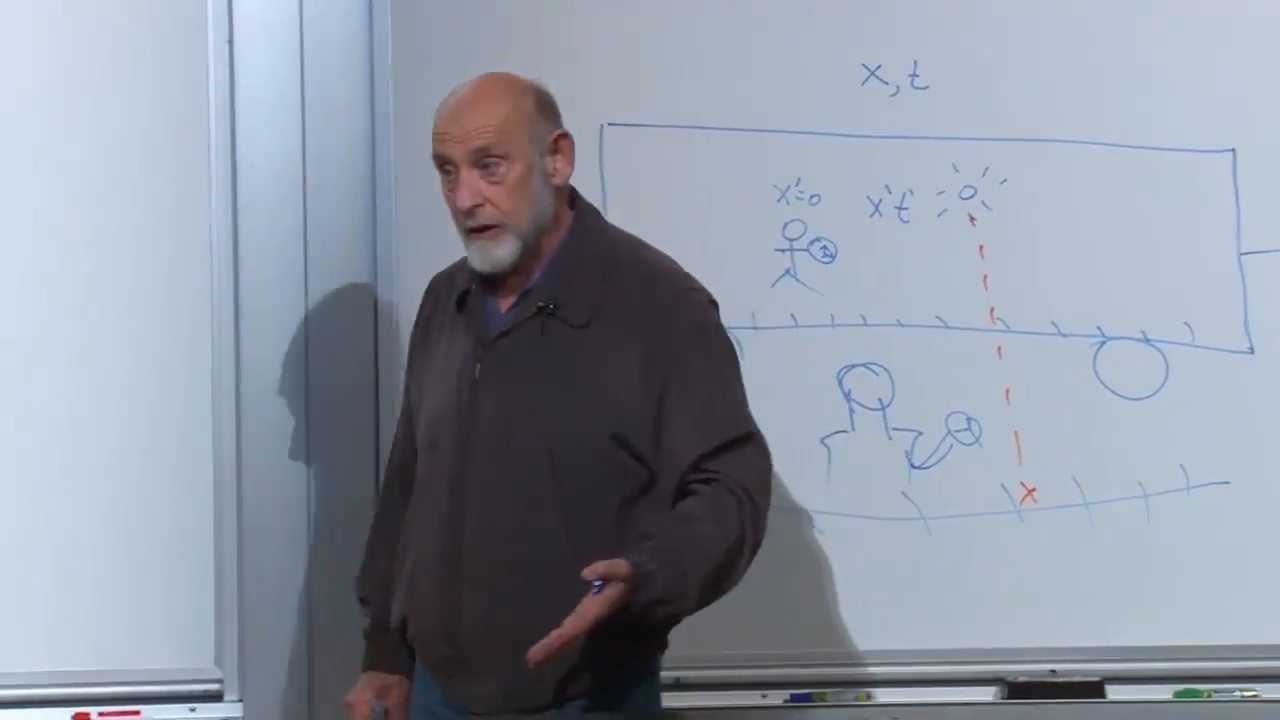
\includegraphics[width=0.90\textwidth]{lecture_02_figure_02.png}
\caption{Die inverse Abbildung hat denselben Lorentzfaktor und das entgegengesetzte Vorzeichen der Relativgeschwindigkeit.}
\lectureframe{00:09:15}
\end{figure}

Bei einem Boost entlang \(x\) ändern sich die transversalen Koordinaten nicht:
\begin{equation}
y'=y,
\qquad
z'=z.
\end{equation}

Die Relativgeschwindigkeit lässt sich aus der Ortsgleichung ablesen, ohne ihren Nenner zu betrachten. Der Zugursprung ist durch \(x'=0\) definiert, also gilt
\begin{equation}
x'=0
\quad\Longleftrightarrow\quad
x-vt=0
\quad\Longleftrightarrow\quad
x=vt.
\label{eq:sr2-origin-worldline}
\end{equation}
Der Koeffizient von \(t\) in dieser Weltlinie ist die Geschwindigkeit des Zuges in den Bahnhofkoordinaten.

\section{Drei Bezugssysteme und die Zusammensetzung von Boosts}

Stellen Sie ein kleines Tretauto in den Zug. Der Zug bewegt sich relativ zum Bahnhof mit der Geschwindigkeit \(v\), während sich das Auto relativ zum Fahrgast mit der Geschwindigkeit \(u\) den Gang entlang bewegt. Die Geschwindigkeit des Autos relativ zum Bahnhof sei \(w\). Nach Newtonscher Intuition wäre \(w=u+v\), doch die Lorentz-Transformationen müssen die Entscheidung liefern.

Nun gibt es drei Koordinatensysteme:
\begin{equation}
(x,t),\qquad (x',t'),\qquad (x'',t'').
\end{equation}
Das erste gehört zum Bahnhof, das zweite zum Zug und das dritte zum Auto. Zwischen Zug und Auto gilt
\begin{align}
x''&=\gamma_u(x'-ut'),&
t''&=\gamma_u(t'-ux'),
\label{eq:sr2-second-boost}\\
\gamma_u&=\frac{1}{\sqrt{1-u^2}}.
\end{align}

\begin{figure}[htbp]
\centering
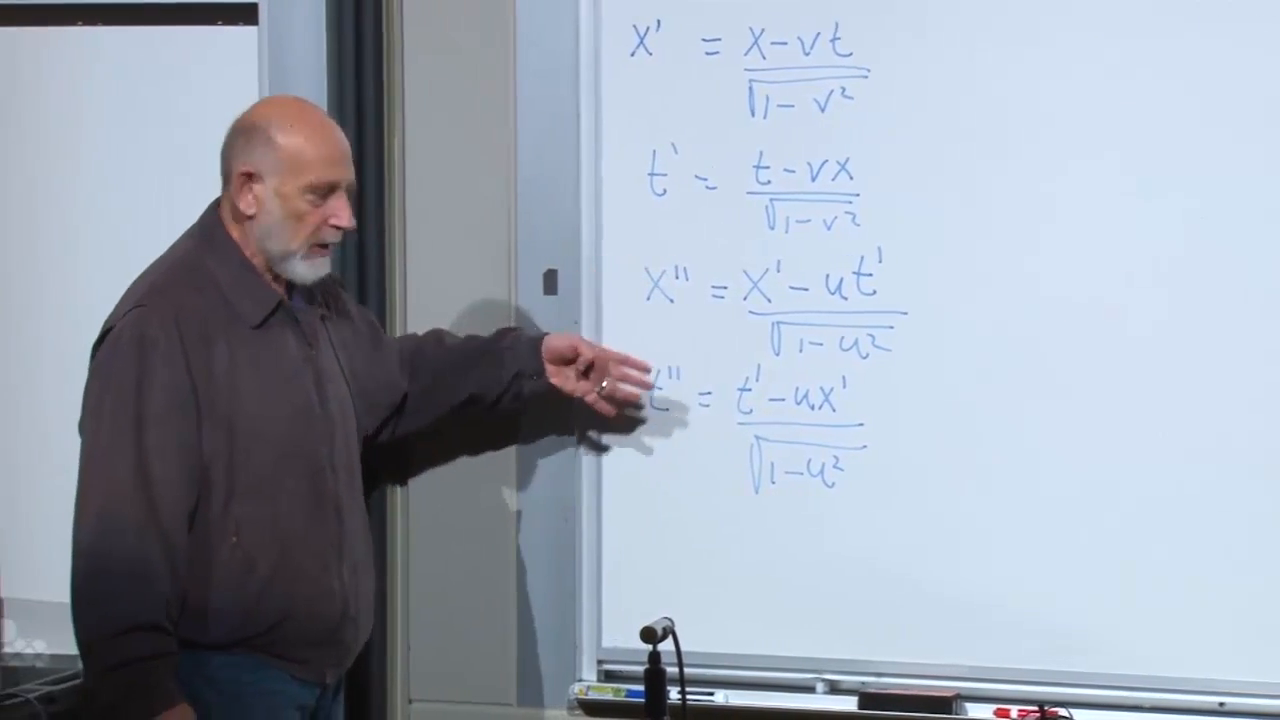
\includegraphics[width=0.90\textwidth]{lecture_02_figure_03.png}
\caption{Auf die direkten Formeln vom Bahnhof zum Zug folgt eine zweite Lorentz-Transformation von gestrichenen zu doppelt gestrichenen Koordinaten.}
\lectureframe{00:14:55}
\end{figure}

\subsection{Einen Boost in den anderen einsetzen}

Um \(w\) zu bestimmen, genügt die Ortsgleichung. Setzen Sie \eqref{eq:sr2-direct} in die erste Gleichung von \eqref{eq:sr2-second-boost} ein:
\begin{align}
x''
&=\gamma_u(x'-ut')\\
&=\gamma_u\gamma_v\left[(x-vt)-u(t-vx)\right]\\
&=\gamma_u\gamma_v\left[(1+uv)x-(u+v)t\right].
\label{eq:sr2-composed-space}
\end{align}
Die beiden Minuszeichen im Term \(uvx\) ergeben ein Pluszeichen; die beiden Zeitanteile fassen sich zu \(-(u+v)t\) zusammen.

\begin{figure}[htbp]
\centering
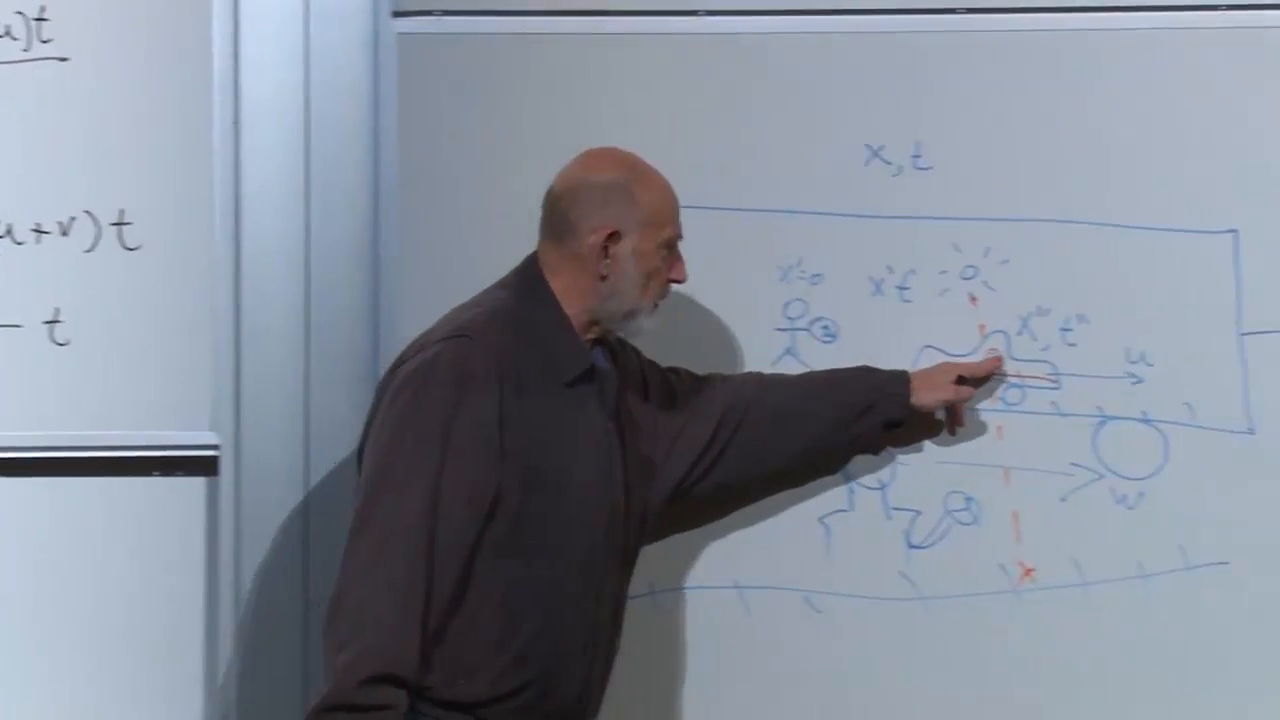
\includegraphics[width=0.91\textwidth]{lecture_02_figure_04.png}
\caption{Die verschachtelte Einsetzung vor dem Zusammenfassen der Terme mit \(x\) und \(t\) im zusammengesetzten Boost.}
\lectureframe{00:16:30}
\end{figure}

Wie zuvor ist der Nenner für die Bestimmung des bewegten Ursprungs unerheblich. Das Tretauto ruht bei \(x''=0\), daher muss die Klammer in \eqref{eq:sr2-composed-space} verschwinden:
\begin{equation}
(1+uv)x-(u+v)t=0.
\end{equation}
Seine Weltlinie im Bahnhofsystem lautet daher
\begin{equation}
x=\frac{u+v}{1+uv}\,t,
\end{equation}
und seine Geschwindigkeit ist
\begin{equation}
\boxed{w=\frac{u+v}{1+uv}}.
\label{eq:sr2-velocity-add-c1}
\end{equation}

\begin{figure}[htbp]
\centering
\includegraphics[width=0.91\textwidth]{lecture_02_figure_05.png}
\caption{Der zusammengefasste Zähler und die Weltlinie \(x=[(u+v)/(1+uv)]t\) geben die zusammengesetzte Geschwindigkeit zu erkennen.}
\lectureframe{00:19:30}
\end{figure}

Auch die Zeitgleichung lässt sich konsistent zusammensetzen. Die vollständige Transformation vom Bahnhof zum Auto hat die Lorentz-Form
\begin{align}
x''&=\gamma_w(x-wt),&
t''&=\gamma_w(t-wx),
\end{align}
mit
\begin{equation}
\gamma_w=\frac{1}{\sqrt{1-w^2}}.
\end{equation}
Tatsächlich gilt
\begin{equation}
\gamma_w=\gamma_u\gamma_v(1+uv),
\end{equation}
Dies folgt, wenn man \eqref{eq:sr2-velocity-add-c1} einsetzt und vereinfacht. Zwei kollineare Boosts ergeben also zusammen wieder einen kollinearen Boost.

\subsection{Dimensionen wiederherstellen}

\begin{classroomqa}
\audiencequestion{Warum ist der Nenner \(1+uv\) in gewöhnlichen Einheiten dimensionswidrig?}
\lecturerresponse{Er ist nur deshalb korrekt, weil \(c=1\) jede Geschwindigkeit zu einem dimensionslosen Bruchteil der Lichtgeschwindigkeit macht. In konventionellen Einheiten muss das Produkt als \(uv/c^2\) auftreten und ist dann dimensionslos. \lecturetimestamp{00:21:11}}
\end{classroomqa}

Das dimensionsbehaftete Gesetz der Geschwindigkeitsaddition lautet
\begin{equation}
\boxed{
w=\frac{u+v}{1+\dfrac{uv}{c^2}}
}.
\label{eq:sr2-velocity-add}
\end{equation}

\begin{figure}[htbp]
\centering
\includegraphics[width=0.90\textwidth]{lecture_02_figure_06.png}
\caption{Aufgrund der Dimensionskonsistenz tritt unter dem Produkt \(uv\) der Faktor \(c^2\) auf.}
\lectureframe{00:22:06}
\end{figure}

Für \(\lvert u\rvert,\lvert v\rvert\ll c\) gilt
\begin{equation}
\frac{uv}{c^2}\ll 1,
\end{equation}
also
\begin{equation}
w\approx u+v.
\end{equation}
Die Newtonsche Addition ist die Näherung für kleine Geschwindigkeiten und keine eigenständige Regel.

\subsection{Zwei numerische Bereiche}

Betrachten wir zunächst
\begin{equation}
u=v=0.01c.
\end{equation}
In den Einheiten \(c=1\) gilt
\begin{equation}
w=\frac{0.02}{1.0001}\approx 0.019998.
\end{equation}
Ein Prozent der Lichtgeschwindigkeit entspricht bereits ungefähr \(3\times10^6\ {\rm m/s}\), dennoch beträgt die relativistische Korrektur nur ein Zehntausendstel. Das Ergebnis ist geringfügig kleiner als die Newtonsche Vorhersage \(0.02c\).

\begin{figure}[htbp]
\centering
\includegraphics[width=0.90\textwidth]{lecture_02_figure_07.png}
\caption{Bei \(u=v=0.01c\) weicht der Nenner nur um \(10^{-4}\) von eins ab.}
\lectureframe{00:24:23}
\end{figure}

Betrachten wir nun
\begin{equation}
u=v=0.9c.
\end{equation}
Nach Newton ergäbe sich \(1.8c\). Die Relativitätstheorie liefert
\begin{equation}
\frac{w}{c}
=\frac{0.9+0.9}{1+0.9^2}
=\frac{1.8}{1.81}
\approx 0.9945.
\label{eq:sr2-fast-example}
\end{equation}

\begin{figure}[htbp]
\centering
\includegraphics[width=0.90\textwidth]{lecture_02_figure_08.png}
\caption{Zwei Geschwindigkeiten von \(0.9c\) ergeben zusammen \(1.8/1.81\), also weiterhin weniger als die Lichtgeschwindigkeit.}
\lectureframe{00:25:48}
\end{figure}

Aufeinanderfolgende unterluminale Boosts können die Lichtgeschwindigkeit \(c\) nicht überschreiten. Wenn \(u<c\) und \(v<c\) gelten, dann gilt
\begin{equation}
1-\frac{w}{c}
=
\frac{\left(1-\frac{u}{c}\right)
      \left(1-\frac{v}{c}\right)}
     {1+\frac{uv}{c^2}}
>0.
\end{equation}
Jeder weitere Boost kann das Ergebnis näher an \(c\) heranbringen, aber niemals darüber hinaus. Für den Grenzwert \(u=c\) gilt
\begin{equation}
w=\frac{c+v}{1+v/c}=c.
\end{equation}
Die Lichtgeschwindigkeit ist ein Fixpunkt des Zusammensetzungsgesetzes.

\section{Koordinatenmessung ist nicht gleich visuelle Erscheinung}

\begin{classroomqa}
\audiencequestion{Wenn der Zug Glaswände hat, könnte der Beobachter am Bahnhof den Fahrgast und das Tretauto dann nicht einfach gemeinsam ansehen und ihre Bewegungen direkt ablesen?}
\lecturerresponse{Die Lorentz-Transformation bezieht sich auf Koordinatenmessungen mit räumlich verteilten Maßstäben und synchronisierten Uhren. Ein visuelles Bild enthält außerdem die unterschiedlichen Laufzeiten des Lichts von verschiedenen Ereignissen bis zum Beobachter. Glas verändert den Anblick, nicht den Koordinatenzusammenhang; ein einzelnes Bild als gleichzeitige Daten zu behandeln, würde genau jene Gleichzeitigkeit voraussetzen, die durch die Relativitätstheorie korrigiert wurde. \lecturetimestamp{00:27:53}}
\end{classroomqa}

Ein Ereignis hat in jedem Bezugssystem einen Ort und eine Zeit, unabhängig davon, ob es gerade jemand sieht. Die optische Erscheinung ist ein legitimer Untersuchungsgegenstand, erfordert aber eine zweite Rechnung, die das Licht von jedem Ereignis bis zum Auge verfolgt. Die Transformationsgesetze selbst sind universell und unabhängig von den Wänden des Zuges.

\section{Das Eigenintervall in drei räumlichen Dimensionen}

Kehren wir zu zwei Ereignissen zurück: Das eine liegt zunächst im Ursprung, das andere bei \((x,t)\). In einer räumlichen Dimension gilt
\begin{equation}
\tau^2=t^2-x^2
\label{eq:sr2-interval-1d}
\end{equation}
in den Einheiten \(c=1\). Alle Inertialsysteme stimmen überein:
\begin{equation}
\tau^2
=t^2-x^2
=t'^2-x'^2
=t''^2-x''^2.
\end{equation}
Die Koordinaten ändern sich, das Eigenintervall bleibt unverändert.

Bei zeitartiger Trennung kann sich eine Uhr zwischen den Ereignissen bewegen. Zeigt sie beim ersten Ereignis Mittag an, so ist die verstrichene Zeit bis zum zweiten Ereignis die Eigenzeit \(\tau\). Diese Aussage ist unabhängig davon, welches Koordinatensystem zur Berechnung des Intervalls verwendet wird.

\begin{figure}[htbp]
\centering
\includegraphics[width=0.90\textwidth]{lecture_02_figure_09.png}
\caption{Zur Erinnerung die invariante Eigenzeitbeziehung \(\tau^2=t^2-x^2\), bevor die transversalen Richtungen wieder einbezogen werden.}
\lectureframe{00:30:18}
\end{figure}

\subsection{Die transversalen Richtungen durch räumliche Drehungen wieder einbeziehen}

Betrachten wir eine gewöhnliche Drehung der räumlichen Achsen, bevor wir zu Boosts zurückkehren. Für einen Punkt, der nicht auf der \(x\)-Achse liegt, beträgt das Quadrat des räumlichen Abstands
\begin{equation}
r^2=x^2+y^2+z^2,
\end{equation}
und bleibt nach dem gewöhnlichen Satz des Pythagoras bei Drehungen invariant. Das \(3+1\)-dimensionale Raumzeitintervall lautet folglich
\begin{equation}
\boxed{
\tau^2=t^2-x^2-y^2-z^2
}.
\label{eq:sr2-interval-3d}
\end{equation}
Mit wiederhergestelltem \(c\) gilt
\begin{equation}
c^2\tau^2
=c^2t^2-x^2-y^2-z^2.
\end{equation}

\begin{figure}[htbp]
\centering
\includegraphics[width=0.90\textwidth]{lecture_02_figure_10.png}
\caption{Der Satz des Pythagoras für den räumlichen Abstand erweitert die Invariante von \(t^2-x^2\) auf \(t^2-x^2-y^2-z^2\).}
\lectureframe{00:34:23}
\end{figure}

Jede Kombination aus räumlichen Drehungen und Lorentz-Boosts lässt \eqref{eq:sr2-interval-3d} invariant. Gewöhnliche Koordinatenachsen können sich über die Komponenten uneinig sein, stimmen aber im euklidischen Abstand überein; Inertialsysteme der Raumzeit können sich über die Raum- und Zeitkomponenten uneinig sein, stimmen aber in dieser Differenz der Quadrate überein. Diese Invariante ist die zentrale geometrische Tatsache der speziellen Relativitätstheorie.

\begin{classroomqa}
\audiencequestion{Erhalten Beobachter im Zug und am Bahnhof dieselbe Lichtgeschwindigkeit, wenn der Fahrgast das Tretauto durch einen nach vorn gerichteten Lichtstrahl ersetzt?}
\lecturerresponse{Setzen Sie \(u=c\) in \eqref{eq:sr2-velocity-add} ein. Dann gilt \(w=(c+v)/(1+v/c)=c\). In den Einheiten \(c=1\) ist das Verhältnis einfach \((1+v)/(1+v)=1\). Beide Bezugssysteme messen dieselbe Geschwindigkeit, genau wie gefordert. \lecturetimestamp{00:35:53}}
\end{classroomqa}

Die frühere Frage zu den Glaswänden zeigt also keinen Fehler bei der Invarianz der Lichtgeschwindigkeit. Sie beruht auf einer Verwechslung von Koordinatenmessung und verzögertem visuellem Bild, letztlich auf einer Verwechslung hinsichtlich der Gleichzeitigkeit.

\section{Nullstrahlen und der Lichtkegel}

In einer Raumdimension erfüllen nach rechts und links laufende Lichtstrahlen
\begin{equation}
x=\pm t.
\end{equation}
Ihr Intervall verschwindet:
\begin{equation}
t^2-x^2=0.
\end{equation}
Anders als beim euklidischen Abstand bedeutet ein verschwindendes Raumzeitintervall nicht, dass die Ereignisse zusammenfallen. Es bedeutet, dass ein Lichtsignal sie miteinander verbinden kann.

Wenn alle räumlichen Richtungen einbezogen werden, gilt für einen Lichtstrahl
\begin{equation}
t^2-x^2-y^2-z^2=0,
\label{eq:sr2-null}
\end{equation}
oder
\begin{equation}
r=t
\end{equation}
für zukunftsgerichtetes Licht in den Einheiten \(c=1\).

\begin{figure}[htbp]
\centering
\includegraphics[width=0.90\textwidth]{lecture_02_figure_11.png}
\caption{Licht breitet sich in jeder räumlichen Richtung entlang einer Nulltrajektorie aus, die \(t^2-(x^2+y^2+z^2)=0\) erfüllt.}
\lectureframe{00:39:28}
\end{figure}

In \(1+1\) Dimensionen besteht die Nullmenge aus einem Paar von Geraden mit einem Winkel von \(45^\circ\). Mit zwei Raumdimensionen und einer Zeitdimension wird daraus ein Kegel; drei Raumdimensionen lassen sich nicht vollständig an einer Tafel darstellen, doch die definierende Gleichung bleibt unverändert.

Der zukünftige Lichtkegel umfasst die Ereignisse, die das am Ursprung ausgesandte Licht erreichen kann. Der vergangene Lichtkegel umfasst die Ereignisse, von denen Licht den Ursprung erreichen kann. Der eine entsteht aus dem anderen durch eine Umkehrung der Zeitrichtung.

\begin{figure}[htbp]
\centering
\includegraphics[width=0.90\textwidth]{lecture_02_figure_12.png}
\caption{Die Nullstrahlen bei \(45^\circ\) bilden in einer höherdimensionalen Raumzeitdarstellung den zukünftigen und den vergangenen Lichtkegel.}
\lectureframe{00:40:47}
\end{figure}

\begin{classroomqa}
\audiencequestion{Welche Größe ist in der Newtonschen Mechanik unter Galilei-Transformationen invariant?}
\lecturerresponse{Das Zeitintervall selbst. Alle Newtonschen Beobachter stimmen über \(\Delta t\) überein, auch wenn sie sich über die räumliche Verschiebung uneinig sind. Die Relativitätstheorie gibt die universelle Zeit auf und ersetzt sie durch das invariante Raumzeitintervall. \lecturetimestamp{00:41:53}}
\end{classroomqa}

\section{Von räumlichen Vektoren zu Vierervektoren}

Die hier betrachteten Vektoren sind geometrische Vektoren, keine Quantenzustandsvektoren. Eine Verschiebung zwischen zwei Punkten im gewöhnlichen Raum hat einen Betrag und eine Richtung. Man kann ihren Anfangspunkt zum Ursprung verschieben, ohne den Vektor zu ändern, und ihre drei Komponenten bezeichnen mit
\begin{equation}
x^i=(x^1,x^2,x^3)=(x,y,z),
\qquad i=1,2,3.
\end{equation}
Der lateinische Index \(i\) läuft nur über die räumlichen Richtungen.

Ein Ereignis benötigt eine zusätzliche Komponente: seine Zeit. Eine Raumzeitposition schreibt man daher als
\begin{equation}
x^\mu=(x^0,x^1,x^2,x^3)=(t,x,y,z),
\qquad \mu=0,1,2,3.
\label{eq:sr2-four-position}
\end{equation}
Historisch bedingt ist die Zeit die nullte statt der vierten Komponente:
\begin{equation}
x^0=t,\qquad x^1=x,\qquad x^2=y,\qquad x^3=z.
\end{equation}
Griechische Indizes wie \(\mu\) laufen über die Raumzeit; lateinische Indizes wie \(i\) über den Raum.

\begin{figure}[htbp]
\centering
\includegraphics[width=0.90\textwidth]{lecture_02_figure_13.png}
\caption{Die räumlichen Komponenten \(x^i\) werden zur vierkomponentigen Raumzeitposition \(x^\mu=(x^0,x^1,x^2,x^3)\) erweitert.}
\lectureframe{00:46:05}
\end{figure}

Die Invariante lautet nun
\begin{equation}
\tau^2
=(x^0)^2-(x^1)^2-(x^2)^2-(x^3)^2.
\end{equation}
Die Notation allein fügt keine neue Physik hinzu. Ihr Vorteil besteht darin, dass eine Lorentz-Transformation linear auf alle vier Komponenten wirkt, so wie eine Drehung linear auf einen räumlichen Vektor wirkt.

\begin{classroomqa}
\audiencequestion{Kann eine lineare Transformation als Matrix dargestellt werden, die auf einen Spaltenvektor wirkt?}
\lecturerresponse{Ja. Bei einem Boost entlang \(x\) wirkt der nichttriviale Block \(\gamma_v\begin{pmatrix}1&-v\\-v&1\end{pmatrix}\) auf \((t,x)^{\mathsf T}\), während \(y\) und \(z\) unverändert bleiben. Die Matrixnotation ist die natürliche Art, Lorentz-Transformationen zusammenzusetzen und zu ordnen. \lecturetimestamp{00:48:14}}
\end{classroomqa}

Explizit gilt
\begin{equation}
\begin{pmatrix}
t'\\x'\\y'\\z'
\end{pmatrix}
=
\begin{pmatrix}
\gamma_v&-\gamma_v v&0&0\\
-\gamma_v v&\gamma_v&0&0\\
0&0&1&0\\
0&0&0&1
\end{pmatrix}
\begin{pmatrix}
t\\x\\y\\z
\end{pmatrix}.
\label{eq:sr2-boost-matrix}
\end{equation}

\section{Verschiebungen und Vierergeschwindigkeit}

Gehen wir von der Position eines Ereignisses zu einem kurzen Abschnitt der Weltlinie eines Teilchens über. Die Viererverschiebung ist
\begin{equation}
\Delta x^\mu
=(\Delta t,\Delta x,\Delta y,\Delta z).
\end{equation}
Wenn eine Verschiebung als klein bezeichnet wird, kommt die Differentialrechnung ins Spiel: Aus \(\Delta x^\mu\) wird \(dx^\mu\). Vorerst macht die endliche Schreibweise die Geometrie anschaulich.

Das Eigenzeitintervall entlang einer zeitartigen Weltlinie erfüllt
\begin{equation}
(\Delta\tau)^2
=(\Delta t)^2-(\Delta x)^2-(\Delta y)^2-(\Delta z)^2.
\label{eq:sr2-proper-increment}
\end{equation}
Die gewöhnliche Geschwindigkeit ist die räumliche Verschiebung geteilt durch die Koordinatenzeit und hat drei Komponenten. Die Vierergeschwindigkeit hingegen ist die Viererverschiebung geteilt durch die invariante Eigenzeit:
\begin{equation}
u^\mu
=\frac{\Delta x^\mu}{\Delta\tau}
\quad\longrightarrow\quad
\boxed{
u^\mu=\frac{dx^\mu}{d\tau}
}.
\label{eq:sr2-four-velocity}
\end{equation}

\begin{figure}[htbp]
\centering
\includegraphics[width=0.90\textwidth]{lecture_02_figure_14.png}
\caption{Ein Weltlinienabschnitt legt \(\Delta x^\mu\), die invariante Größe \(\Delta\tau\) und die Vierergeschwindigkeit \(u^\mu=\Delta x^\mu/\Delta\tau\) fest.}
\lectureframe{00:52:42}
\end{figure}

Dieses Objekt hat vier Komponenten und transformiert sich wie ein Vierervektor. Wie es mit der gewöhnlichen Dreiergeschwindigkeit zusammenhängt, ist die nächste Frage, die hier bewusst offenbleibt. Ihre Klärung führt zur relativistischen Impuls-, Energie- und Beschleunigungslehre und schließlich zur relativistischen Verallgemeinerung von \(F=ma\).
\graphicspath{{../../../generated_course_notes/core/special_relativity/2012_spring_theoretical_minimum/chapters/lecture_03/}{../../../generated_course_notes/core/special_relativity/2012_spring_theoretical_minimum/figures/}{../../../generated_course_notes/core/special_relativity/2012_spring_theoretical_minimum/assets/}}
\chapter{Teilchenmechanik, Viererimpuls und Ruheenergie}

\section{Die Näherung, die wir immer wieder verwenden werden}

Die Mechanik eines relativistischen Teilchens muss vertraute Fragen in einer neuen Sprache beantworten. Wie bewegt sich ein Teilchen? Was sind sein Impuls und seine Energie? Warum bilden diese Größen zusammen einen Vierervektor, und wie ergibt sich \(E=mc^2\) aus den gewöhnlichen Methoden der Mechanik? Bevor wir uns diesen Fragen zuwenden, benötigen wir eine elementare Näherung, die in der gesamten Rechnung immer wieder auftreten wird.

Für jeden Exponenten \(p\) lautet die Binomialreihe
\begin{equation}
\begin{aligned}
(1+\epsilon)^p
&=1+p\epsilon\\
&\quad+\frac{p(p-1)}{2!}\epsilon^2\\
&\quad+\frac{p(p-1)(p-2)}{3!}\epsilon^3
+\cdots .
\end{aligned}
\label{eq:sr3-binomial}
\end{equation}
Der Exponent kann positiv, negativ, gebrochen oder sogar komplex sein. Für hinreichend kleines \(\epsilon\) konvergiert die Reihe schnell, und jeder folgende Term ist kleiner. Dann können wir die Entwicklung bei derjenigen Ordnung abbrechen, die für die gewünschte Genauigkeit erforderlich ist. Der Term nullter Ordnung ist oft der größte, in den folgenden Anwendungen jedoch häufig eine Konstante und damit dynamisch uninteressant. In der ersten Korrektur kommt die Bewegung zum Ausdruck.

\begin{figure}[htbp]
\centering
\includegraphics[width=0.90\textwidth]{lecture_03_figure_01.png}
\caption{Die Binomialreihe bis zur dritten Ordnung, mit der sich die nichtrelativistische Mechanik aus relativistischen Formeln zurückgewinnen lässt.}
\lectureframe{00:04:24}
\end{figure}

Wir setzen gewöhnlich \(c=1\), sodass eine Geschwindigkeit \(v\) den Anteil \(v/c\) der Lichtgeschwindigkeit bezeichnet. Setzen wir \(\epsilon=-v^2\). Mit \(p=\tfrac12\) gilt:
\begin{equation}
\sqrt{1-v^2}
=
1-\frac{v^2}{2}-\frac{v^4}{8}-\cdots
\approx
1-\frac{v^2}{2},
\qquad |v|\ll 1.
\label{eq:sr3-sqrt-expansion}
\end{equation}
Bei \(p=-\tfrac12\) heben sich die beiden Minuszeichen auf:
\begin{equation}
\frac{1}{\sqrt{1-v^2}}
=
1+\frac{v^2}{2}+\frac{3v^4}{8}+\cdots
\approx
1+\frac{v^2}{2}.
\label{eq:sr3-gamma-expansion}
\end{equation}
Viele Faktoren \(1/2\) in der klassischen Mechanik lassen sich im Nachhinein als erste Korrektur einer dieser relativistischen Entwicklungen erkennen. Die Näherung versagt, wenn \(v\) gegen eins geht; dann kann kein Abbruch nach endlich vielen Termen das singuläre Verhalten des exakten Ausdrucks erfassen.

\begin{figure}[htbp]
\centering
\includegraphics[width=0.90\textwidth]{lecture_03_figure_02.png}
\caption{Beide Formeln für kleine Geschwindigkeiten sind zu sehen: \(\sqrt{1-v^2}\approx1-v^2/2\) und \((1-v^2)^{-1/2}\approx1+v^2/2\).}
\lectureframe{00:07:39}
\end{figure}

\section{Was gilt als Teilchen?}

Ein Teilchen in der Mechanik muss nicht elementar sein. Es kann ein Elektron, die Sonne, eine Pralinenschachtel oder ein Donut sein. Entscheidend ist, dass das Objekt hinreichend gut zusammenhält, sodass sich seine Gesamtbewegung durch einen Schwerpunkt beschreiben lässt. Ein Donut erinnert daran, dass der Schwerpunkt nicht im materiellen Teil des Körpers liegen muss.

In der Newtonschen Mechanik erfüllen die Schwerpunktgrößen
\begin{equation}
\vec p=m\vec v,
\qquad
K=\frac12mv^2,
\qquad
\vec F=m\vec a.
\label{eq:sr3-newtonian-particle}
\end{equation}
Diese Formeln gelten unabhängig davon, ob das Objekt elementar oder zusammengesetzt ist. Ein zusammengesetztes Objekt besitzt außerdem innere Energie. Ein bewegter Donut hat zum Beispiel neben der kinetischen Energie seines Schwerpunkts auch chemische, thermische und Bindungsenergie:
\begin{equation}
E_{\text{Newtonian}}
=
E_{\text{internal}}+\frac12mv^2.
\label{eq:sr3-newtonian-internal}
\end{equation}
Der innere Anteil hängt nicht von der Gesamtgeschwindigkeit des Schwerpunkts ab. Die Relativitätstheorie behält diese Unterscheidung bei, zeigt aber, dass die innere Energie zur invarianten Masse des gesamten Objekts beiträgt.

Wir benötigen dieselben Werkzeuge wie in der klassischen Mechanik: Trajektorien, das Prinzip der stationären Wirkung, Lagrange-Funktionen, kanonische Impulse, Hamilton-Funktionen und den Zusammenhang zwischen kontinuierlichen Symmetrien und Erhaltungssätzen.

\section{Weltlinien und kausale Trennung}

Tragen wir die Position eines Systems horizontal und die Zeit vertikal auf. Seine Geschichte bildet dann eine Kurve in der Raumzeit. Für ein Teilchen heißt diese Kurve seine \emph{Weltlinie}. Das Konzept gibt es bereits in der Newtonschen Mechanik, doch in der Relativitätstheorie wird es grundlegend, weil Lorentz-Transformationen Raum und Zeit miteinander vermischen.

Betrachten wir zwei Ereignisse mit dem Abstand
\begin{equation}
\Delta x^\mu=(\Delta t,\Delta\vec x),
\qquad
\Delta\vec x^{\,2}
=
(\Delta x)^2+(\Delta y)^2+(\Delta z)^2.
\end{equation}
In Einheiten \(c=1\) ist ihr invariantes Intervall
\begin{equation}
(\Delta\tau)^2
=
(\Delta t)^2-\Delta\vec x^{\,2}.
\label{eq:sr3-interval}
\end{equation}

\subsection{Zeitartige Trennung}

Wenn \((\Delta t)^2>\Delta\vec x^{\,2}\) gilt, dann gilt \((\Delta\tau)^2>0\), und die Trennung ist zeitartig. Es gibt ein Lorentz-System, in dem die beiden Ereignisse am selben räumlichen Ort stattfinden. In diesem System ist die Verbindungslinie zwischen ihnen vertikal, und eine Uhr kann von einem Ereignis zum anderen gelangen. Ihre verstrichene Anzeige ist die Eigenzeit \(\Delta\tau\).

\begin{figure}[htbp]
\centering
\includegraphics[width=0.90\textwidth]{lecture_03_figure_03.png}
\caption{Bei einem zeitartigen Intervall ist die zeitliche Trennung größer als die räumliche; es gibt ein Ruhesystem, in dem beide Ereignisse am selben Ort stattfinden.}
\lectureframe{00:14:42}
\end{figure}

\subsection{Raumartige Trennung}

Wenn \(\Delta\vec x^{\,2}>(\Delta t)^2\) gilt, ist das Intervall raumartig. Kein Inertialsystem bringt beide Ereignisse an denselben räumlichen Ort, aber es gibt ein System, in dem sie gleichzeitig stattfinden. In anderen Systemen kann sich ihre zeitliche Reihenfolge umkehren. Daher ist für ein raumartiges Ereignispaar weder die Aussage, \emph{Ereignis \(A\) habe zuerst stattgefunden}, noch die Aussage, \emph{Ereignis \(B\) habe zuerst stattgefunden}, invariant. Dies ist die Relativität der Gleichzeitigkeit in geometrischer Form.

\begin{figure}[htbp]
\centering
\includegraphics[width=0.90\textwidth]{lecture_03_figure_04.png}
\caption{Bei einem raumartigen Intervall kann ein Wechsel des Inertialsystems die beiden Ereignisse gleichzeitig machen oder ihre zeitliche Reihenfolge umkehren.}
\lectureframe{00:17:01}
\end{figure}

Ein massives Teilchen hat eine zeitartige Weltlinie: Jedes hinreichend kurze Segment erfüllt \(d\tau^2>0\). Durch fortgesetztes Zusammensetzen von Geschwindigkeiten der Größe \(0.9c\) kann sich ein Teilchen \(c\) immer weiter nähern, es aber nie überschreiten. Die Annäherung erinnert an Zenons Paradoxon. Diese Kausalitätsbeschränkung gilt nicht nur für materielle Objekte, sondern auch für Signale und Information, denn Information muss von physikalischen Systemen übertragen werden. Ein Signal, das sich schneller als Licht ausbreitet, würde es verschiedenen Bezugssystemen ermöglichen, darüber uneinig zu sein, welches Ende seiner Geschichte Ursache und welches Wirkung ist.

\section{Vierergeschwindigkeit}

Betrachten wir ein kurzes zeitartiges Segment. In konventionellen Einheiten gilt
\begin{equation}
d\tau
=
\sqrt{dt^2-\frac{d\vec x^{\,2}}{c^2}}.
\label{eq:sr3-proper-time-dimensional}
\end{equation}
Der Faktor \(c^2\) ist durch die Dimensionen vorgegeben: \(dt^2\) hat die Einheit einer Zeit zum Quadrat, während \(d\vec x^{\,2}\) die Einheit einer Länge zum Quadrat hat.

\begin{classroomqa}
\audiencequestion{Wo muss die Lichtgeschwindigkeit eingesetzt werden, wenn das Intervall in gewöhnlichen Einheiten angegeben wird?}
\lecturerresponse{Der räumliche Term muss durch \(c^2\) geteilt werden, sodass sich \(d\tau^2=dt^2-d\vec x^{\,2}/c^2\) ergibt. In der Regel verwenden wir wieder \(c=1\), doch aus der Dimensionskonsistenz lassen sich die fehlenden Faktoren stets wiederherstellen. \lecturetimestamp{00:21:23}}
\end{classroomqa}

\begin{figure}[htbp]
\centering
\includegraphics[width=0.90\textwidth]{lecture_03_figure_05.png}
\caption{Eine Weltlinienverschiebung \(\Delta x^\mu=(\Delta t,\Delta\vec x)\) und der zugehörige Eigenzeitabschnitt.}
\lectureframe{00:21:03}
\end{figure}

Die gewöhnliche Geschwindigkeit hat drei räumliche Komponenten,
\begin{equation}
v^i=\frac{dx^i}{dt},
\qquad i=1,2,3.
\end{equation}
Die relativistische Geschwindigkeit erhält man, indem man die gesamte Raumzeitverschiebung durch die invariante Eigenzeit teilt:
\begin{equation}
u^\mu
=
\frac{dx^\mu}{d\tau},
\qquad
\mu=0,1,2,3.
\label{eq:sr3-four-velocity-definition}
\end{equation}
Griechische Indizes durchlaufen die Raumzeit, lateinische Indizes den Raum. Die nullte Positionskomponente ist in Einheiten \(c=1\) gleich \(x^0=t\), also
\begin{equation}
u^0=\frac{dt}{d\tau}.
\end{equation}

\begin{figure}[htbp]
\centering
\includegraphics[width=0.90\textwidth]{lecture_03_figure_06.png}
\caption{Die gewöhnliche Geschwindigkeit ist die räumliche Verschiebung geteilt durch die Koordinatenzeit; die Vierergeschwindigkeit erhält man, indem man alle vier Komponenten durch die Eigenzeit teilt.}
\lectureframe{00:24:05}
\end{figure}

Um \(u^\mu\) mit \(\vec v\) in Beziehung zu setzen, klammern wir \(dt^2\) im Intervall aus:
\begin{align}
d\tau^2
&=dt^2-d\vec x^{\,2}\\
&=dt^2\left(1-\frac{d\vec x^{\,2}}{dt^2}\right)
=dt^2(1-v^2).
\end{align}
Für eine zukunftsgerichtete Weltlinie wählen wir die positive Wurzel:
\begin{equation}
\frac{d\tau}{dt}=\sqrt{1-v^2},
\qquad
\frac{dt}{d\tau}=\frac{1}{\sqrt{1-v^2}}
\equiv\gamma.
\label{eq:sr3-time-component}
\end{equation}
Für eine räumliche Komponente gilt
\begin{equation}
v^i
=
\frac{dx^i}{dt}
=
\frac{dx^i}{d\tau}\frac{d\tau}{dt}
=u^i\sqrt{1-v^2}.
\end{equation}
Damit folgt
\begin{equation}
\boxed{
u^\mu
=
\gamma(1,\vec v)
},
\qquad
u^0=\gamma,
\qquad
u^i=\gamma v^i.
\label{eq:sr3-four-velocity-components}
\end{equation}
Bei kleinen Geschwindigkeiten gilt \(u^0\to1\) und \(u^i\to v^i\). In der Nähe der Lichtgeschwindigkeit werden sowohl \(u^0\) als auch der Betrag der räumlichen Vierergeschwindigkeit groß, obwohl \(|\vec v|<1\).

\begin{figure}[htbp]
\centering
\includegraphics[width=0.90\textwidth]{lecture_03_figure_07.png}
\caption{Der endgültige Zusammenhang zwischen der gewöhnlichen Geschwindigkeit und allen vier Komponenten von \(u^\mu\).}
\lectureframe{00:30:40}
\end{figure}

\subsection{Warum nur drei Komponenten unabhängig sind}

Die Vierergeschwindigkeit hat vier Komponenten, aber nur drei unabhängige Freiheitsgrade. Teilt man die Intervallgleichung durch \(d\tau^2\), erhält man
\begin{equation}
1
=
\left(\frac{dt}{d\tau}\right)^2
-\left(\frac{d\vec x}{d\tau}\right)^2,
\end{equation}
oder
\begin{equation}
\boxed{
(u^0)^2-\vec u^{\,2}=1
}.
\label{eq:sr3-four-velocity-normalization}
\end{equation}
Die eine Normierungsbedingung beseitigt eine unabhängige Komponente.

\begin{figure}[htbp]
\centering
\includegraphics[width=0.90\textwidth]{lecture_03_figure_08.png}
\caption{Aus dem invarianten Intervall folgt unmittelbar die Normierung \((u^0)^2-\vec u^{\,2}=1\).}
\lectureframe{00:33:50}
\end{figure}

\begin{classroomqa}
\audiencequestion{Lässt sich der Verlust einer unabhängigen Komponente dadurch verstehen, dass man nach der Eigenzeit selbst ableitet?}
\lecturerresponse{Ja. Die Eigenzeit ist keine unabhängige fünfte Koordinate; sie wird durch das Raumzeitintervall entlang der Weltlinie festgelegt. Teilt man diese definierende Beziehung durch \(d\tau^2\), so müssen die vier Ableitungen auf dem Einheits-Hyperboloid zeitartiger Vektoren \((u^0)^2-\vec u^{\,2}=1\) liegen. \lecturetimestamp{00:34:07}}
\end{classroomqa}

\section{Eine invariante Wirkung für ein freies Teilchen}

Welches Gesetz bestimmt eine kraftfreie Weltlinie? Wir übernehmen zwei Erkenntnisse aus der klassischen Mechanik:
\begin{enumerate}
\item Der physikalische Weg macht die Wirkung stationär, während die Endpunkte festgehalten werden;
\item die Wirkung setzt sich additiv aus infinitesimalen Wegsegmenten zusammen.
\end{enumerate}
Die Relativitätstheorie stellt eine dritte Forderung: Alle Inertialbeobachter müssen derselben Wirkung zustimmen. Die naheliegende infinitesimale skalare Größe auf einer zeitartigen Weltlinie ist \(d\tau\). Daher lautet die Wirkung eines freien Teilchens
\begin{equation}
\boxed{
S=-m\int_a^b d\tau
}
\qquad(c=1).
\label{eq:sr3-invariant-action}
\end{equation}
Das Bild einer endlichen Summe lautet
\begin{equation}
S=-m\lim_{N\to\infty}\sum_{k=1}^{N}\Delta\tau_k.
\end{equation}
Da alle Beobachter jedem Eigenzeitabschnitt zustimmen, stimmen sie auch darin überein, welcher Weg ihre Summe stationär macht.

\begin{figure}[htbp]
\centering
\includegraphics[width=0.90\textwidth]{lecture_03_figure_09.png}
\caption{Die Wirkung wird als Summe invarianten Eigenzeitabschnitte entlang einer variierten Weltlinie mit festen Endpunkten gebildet.}
\lectureframe{00:38:30}
\end{figure}

\begin{classroomqa}
\audiencequestion{Was geschieht mit der Energie, wenn die Wirkung mit einer beliebigen Konstante multipliziert wird?}
\lecturerresponse{Die Energie ist keine Ausgangsinvariante; sie wird aus der Lagrange-Funktion und der Hamilton-Funktion hergeleitet. Wird die gesamte Wirkung mit einer von null verschiedenen Konstante multipliziert, bleiben ihre stationären Wege unverändert, auch wenn sich dadurch die aus dieser Wirkung definierten kanonischen Größen skalieren. Die Normierung \(-m\) wird so gewählt, dass diese abgeleiteten Größen den etablierten Newtonschen Konventionen entsprechen. \lecturetimestamp{00:39:47}}
\end{classroomqa}

\begin{classroomqa}
\audiencequestion{Warum eignet sich eine Invariante wie die Eigenzeit als Grundlage für die Wirkung?}
\lecturerresponse{Ein Gesetz der stationären Wirkung sollte in jedem Inertialsystem denselben physikalischen Weg auswählen. Das ist vergleichbar mit der Suche nach der kürzesten Kurve in einer euklidischen Ebene: Drehungen ändern die Koordinatenkomponenten, aber nicht die infinitesimale Länge und somit auch nicht, welche Kurve die kürzeste ist. Ersetzt man die euklidische Länge durch die Eigenzeit, erhält man die relativistische Konstruktion. \lecturetimestamp{00:40:39}}
\end{classroomqa}

\begin{classroomqa}
\audiencequestion{Warum wählen wir für die Eigenzeit die positive statt der negativen Quadratwurzel?}
\lecturerresponse{Die Eigenzeit ist als positive verstrichene Anzeige einer Uhr definiert, die von der Vergangenheit in die Zukunft getragen wird. Eine konsequente Wahl der negativen Wurzel würde lediglich das Vorzeichen der Wirkung umkehren und aus einem Minimum ein Maximum machen, ohne die stationäre Weltlinie zu ändern. Im Ruhesystem der Uhr ergibt die positive Konvention \(d\tau=dt\). \lecturetimestamp{00:42:59}}
\end{classroomqa}

Auch der Faktor \(-m\) ist eine Normierungskonvention, die so gewählt wird, dass sich die Newtonsche Mechanik zurückgewinnen lässt. In Einheiten mit Dimensionen lautet die konventionelle Wirkung
\begin{equation}
S=-mc^2\int_a^b d\tau.
\label{eq:sr3-action-dimensional}
\end{equation}

\begin{figure}[htbp]
\centering
\includegraphics[width=0.90\textwidth]{lecture_03_figure_10.png}
\caption{Die endliche Summe der Eigenzeiten wird in natürlichen Einheiten zum invarianten Integral \(-m\int d\tau\).}
\lectureframe{00:46:23}
\end{figure}

\section{Die relativistische Lagrange-Funktion}

Um die Wirkung in die übliche mechanische Form zu bringen, klammern wir \(dt\) aus \(d\tau\) aus:
\begin{equation}
d\tau
=dt\sqrt{1-\dot{\vec x}^{\,2}},
\qquad
\dot{\vec x}^{\,2}
=\dot x^2+\dot y^2+\dot z^2.
\end{equation}
Dann gilt
\begin{equation}
S
=
\int_a^b L\,dt,
\qquad
\boxed{
L=-m\sqrt{1-v^2}
}
\quad(c=1).
\label{eq:sr3-relativistic-lagrangian}
\end{equation}
In konventionellen Einheiten gilt
\begin{equation}
L=-mc^2\sqrt{1-\frac{v^2}{c^2}}.
\label{eq:sr3-relativistic-lagrangian-c}
\end{equation}
Dies ist die Lagrange-Funktion eines freien Teilchens: Sie hängt von der Geschwindigkeit, nicht aber vom Ort ab. Eine Kraft oder ein Potential wurde noch nicht eingeführt.

\begin{figure}[htbp]
\centering
\includegraphics[width=0.90\textwidth]{lecture_03_figure_11.png}
\caption{Das Ausklammern von \(dt\) macht die freie relativistische Lagrange-Funktion als Funktion der drei Geschwindigkeitskomponenten sichtbar.}
\lectureframe{00:49:57}
\end{figure}

\subsection{Lagrange und Newton zurückgewinnen}

Setzen wir \eqref{eq:sr3-sqrt-expansion} ein:
\begin{align}
L
&=-m\sqrt{1-v^2}\\
&\approx-m\left(1-\frac{v^2}{2}\right)\\
&=-m+\frac12mv^2.
\label{eq:sr3-lagrangian-low-speed}
\end{align}
Die Konstante \(-m\) hängt weder vom Ort noch von der Geschwindigkeit ab. Sie trägt für jeden Weg mit denselben Endzeitpunkten denselben Betrag bei und fällt daher aus den Euler--Lagrange-Gleichungen heraus. Der dynamisch relevante Anteil ist genau
\begin{equation}
L_{\mathrm{Newton}}=\frac12mv^2.
\end{equation}
Damit wurden Vorzeichen und Massennormierung in der invarianten Wirkung richtig gewählt.

\begin{figure}[htbp]
\centering
\includegraphics[width=0.90\textwidth]{lecture_03_figure_12.png}
\caption{Die Entwicklung für kleine Geschwindigkeiten ergibt die Konstante \(-m\) und die Newtonsche Lagrange-Funktion des freien Teilchens \(mv^2/2\).}
\lectureframe{00:53:24}
\end{figure}

Für das hier betrachtete freie Teilchen besagen die Euler--Lagrange-Gleichungen lediglich, dass die Geschwindigkeit konstant und die Raumzeit-Weltlinie gerade ist. Aufschlussreicher ist es, den erhaltenen Impuls und die erhaltene Energie zu bestimmen.

\section{Kanonischer Impuls}

Da \(L\) nicht vom Ort abhängt, ist sie unter räumlichen Translationen invariant. Die zugehörige Erhaltungsgröße ist der Impuls. Wir setzen die Newtonsche Formel \(p_i=mv_i\) nicht voraus, sondern verwenden die kanonische Definition
\begin{equation}
p_i=\frac{\partial L}{\partial\dot x^i}.
\label{eq:sr3-canonical-momentum}
\end{equation}
Für \(L=-m\sqrt{1-v^2}\) gilt
\begin{align}
p_i
&=
-m\frac{1}{2\sqrt{1-v^2}}
\frac{\partial}{\partial\dot x^i}(1-v^2)\\
&=
-m\frac{1}{2\sqrt{1-v^2}}(-2\dot x^i)\\
&=
\frac{mv_i}{\sqrt{1-v^2}}
=m\gamma v_i.
\label{eq:sr3-relativistic-momentum}
\end{align}
Da \(u^i=\gamma v^i\),
\begin{equation}
\boxed{
p^i=mu^i
}.
\label{eq:sr3-momentum-spatial}
\end{equation}
Bei kleinen Geschwindigkeiten vereinfacht sich dies zu \(p^i\approx mv^i\). In der Nähe der Lichtgeschwindigkeit ist der Nenner entscheidend.

\begin{figure}[htbp]
\centering
\includegraphics[width=0.90\textwidth]{lecture_03_figure_13.png}
\caption{Die kanonische Ableitung der Wurzel-Lagrange-Funktion ergibt \(p_x=mv_x/\sqrt{1-v^2}\).}
\lectureframe{00:58:49}
\end{figure}

\subsection{Masse, nicht relativistische Masse}

Hier ist \(m\) einfach die Masse des Teilchens: eine invariante Kennzeichnung, die sich bei seiner Bewegung nicht ändert. Ältere Texte nennen sie manchmal \emph{Ruhemasse} und bezeichnen \(E/c^2\) als geschwindigkeitsabhängige \emph{relativistische Masse}. Im heutigen Sprachgebrauch vermeidet man diese Unterscheidung. Die Bewegung ändert Energie und Impuls, nicht aber die invariante Masse. Die Masse eines Elektrons ist in jedem Bezugssystem derselbe Parameter.

\section{Vom Dreierimpuls zum Viererimpuls}

Eine Aussage über eine einzelne Komponente eines Vierervektors hängt im Allgemeinen vom Bezugssystem ab. Zum Beispiel besagt \(\Delta\vec x=0\), dass zwei Ereignisse in einem Bezugssystem denselben Ort haben; ein Boost neigt dieses Intervall jedoch und führt zu \(\Delta\vec x'\ne0\). Dagegen ist
\begin{equation}
\Delta x^\mu=0
\end{equation}
invariant: Wenn alle vier Komponenten in einem Bezugssystem verschwinden, verschwinden sie in jedem Bezugssystem. Ebenso kennzeichnet \(\vec u=0\) lediglich das Ruhesystem des Teilchens; es ist keine invariante Beschreibung der Vierergeschwindigkeit.

Für ein abgeschlossenes System lautet die gewöhnliche Impulserhaltung
\begin{equation}
\vec P_{\mathrm{initial}}-\vec P_{\mathrm{final}}=0.
\label{eq:sr3-three-momentum-conservation}
\end{equation}
Dies ist eine Gleichung für Dreiervektoren. Um die Erhaltung manifest lorentzkovariant zu formulieren, benötigen wir eine vierte Komponente, die sich zu den drei Komponenten \(p^i=mu^i\) gesellt. Die naheliegende Ergänzung lautet
\begin{equation}
p^\mu=mu^\mu.
\label{eq:sr3-four-momentum}
\end{equation}
In Einheiten \(c=1\) gilt
\begin{equation}
p^\mu=(p^0,\vec p)
=
m\gamma(1,\vec v).
\end{equation}

\begin{figure}[htbp]
\centering
\includegraphics[width=0.90\textwidth]{lecture_03_figure_14.png}
\caption{Die Impulserhaltung wird erst invariant, wenn die räumlichen Komponenten durch eine vierte Komponente ergänzt werden.}
\lectureframe{01:09:51}
\end{figure}

Die fehlende Komponente muss selbst erhalten sein. Die Teilchenmechanik kennt bereits eine weitere erhaltene Größe: die Energie. Die Frage ist, ob \(p^0=mu^0=m\gamma\) in natürlichen Einheiten genau dieser Energie entspricht. Die systematische Antwort liefert die Hamilton-Funktion.

\section{Die Hamilton-Funktion ist die Energie}

Für jede zeitunabhängige Lagrange-Funktion dieser Form lautet die Hamilton-Funktion
\begin{equation}
H=\sum_{i=1}^{3}\dot x^i p_i-L.
\label{eq:sr3-hamiltonian-definition}
\end{equation}
Diese Formel ist nicht spezifisch für die Newtonsche Mechanik. Sie ist die allgemeine Legendre-Transformation von den Geschwindigkeiten zu den kanonischen Impulsen und gilt ebenso für die relativistische Lagrange-Funktion.

\begin{figure}[htbp]
\centering
\includegraphics[width=0.90\textwidth]{lecture_03_figure_15.png}
\caption{Die allgemeine Formel für die Hamilton-Funktion \(H=\sum_i\dot x^i p_i-L\).}
\lectureframe{01:11:55}
\end{figure}

Setzen wir \(p_i=m\dot x_i/\sqrt{1-v^2}\) und \(L=-m\sqrt{1-v^2}\) ein:
\begin{align}
H
&=
\frac{mv^2}{\sqrt{1-v^2}}
+m\sqrt{1-v^2}\\
&=
\frac{mv^2+m(1-v^2)}{\sqrt{1-v^2}}\\
&=
\boxed{\frac{m}{\sqrt{1-v^2}}}
=m\gamma.
\label{eq:sr3-hamiltonian-result}
\end{align}
Die Aufhebung ist der entscheidende Schritt. Im Vergleich mit \(u^0=\gamma\) gilt
\begin{equation}
H=mu^0=p^0.
\end{equation}
Damit ist die vierte Komponente die Energie:
\begin{equation}
p^\mu=(E,\vec p),
\qquad
E=H
\qquad(c=1).
\label{eq:sr3-four-momentum-natural}
\end{equation}

\begin{figure}[htbp]
\centering
\includegraphics[width=0.90\textwidth]{lecture_03_figure_16.png}
\caption{Die beiden Terme der Hamilton-Funktion werden auf einen gemeinsamen Nenner gebracht; die Beiträge \(mv^2\) heben sich auf.}
\lectureframe{01:14:28}
\end{figure}

\begin{classroomqa}
\audiencequestion{Ist die Formel \(H=\sum_i\dot x^i p_i-L\) nur die klassische Formel für die Hamilton-Funktion?}
\lecturerresponse{Sie ist die allgemeine Legendre-Transformation zu einer Lagrange-Funktion und keine besondere nichtrelativistische Annahme. Die Form von \(L\) entscheidet darüber, welche Mechanik sich ergibt. Hier liefert die relativistische Wurzel-Lagrange-Funktion \(H=m/\sqrt{1-v^2}\). \lecturetimestamp{01:15:21}}
\end{classroomqa}

Die invariante Erhaltungsgleichung lautet nun
\begin{equation}
\sum_{\mathrm{initial}}p^\mu
=
\sum_{\mathrm{final}}p^\mu,
\label{eq:sr3-four-momentum-conservation}
\end{equation}
Sie enthält die Erhaltung der Energie und aller drei Impulskomponenten in einer einzigen Vierervektorgleichung.

\section{Ruheenergie und Newtonscher Grenzfall}

In natürlichen Einheiten ist die exakte Energie
\begin{equation}
E=\frac{m}{\sqrt{1-v^2}}.
\end{equation}
Unter Verwendung von \eqref{eq:sr3-gamma-expansion} folgt
\begin{equation}
E
\approx
m+\frac12mv^2+\frac38mv^4+\cdots .
\label{eq:sr3-energy-natural-expansion}
\end{equation}
Der zweite Term ist die vertraute kinetische Energie. Der erste Term ist die Energie, die verbleibt, wenn der Schwerpunkt ruht.

\begin{figure}[htbp]
\centering
\includegraphics[width=0.90\textwidth]{lecture_03_figure_17.png}
\caption{Die Entwicklung der exakten Energie lautet \(m+mv^2/2+\cdots\) in Einheiten \(c=1\).}
\lectureframe{01:18:02}
\end{figure}

Stellen wir die Dimensionen im exakten Ausdruck wieder her. Der Quotient unter der Wurzel muss \(v^2/c^2\) sein, und der Zähler muss die Einheit einer Energie haben:
\begin{equation}
\boxed{
E
=
\gamma mc^2
=
\frac{mc^2}{\sqrt{1-v^2/c^2}}
}.
\label{eq:sr3-energy-exact}
\end{equation}
Die Entwicklung für kleine Geschwindigkeiten lautet
\begin{equation}
\boxed{
E
=
mc^2+\frac12mv^2
+\frac38m\frac{v^4}{c^2}
+\cdots
}.
\label{eq:sr3-energy-dimensional-expansion}
\end{equation}
In Ruhe gilt
\begin{equation}
\boxed{E_{\mathrm{rest}}=mc^2}.
\label{eq:sr3-emc2}
\end{equation}

\begin{figure}[htbp]
\centering
\includegraphics[width=0.90\textwidth]{lecture_03_figure_18.png}
\caption{Nach Wiederherstellung der Dimensionen wird der konstante Term zu \(mc^2\), gefolgt von der Newtonschen kinetischen Energie \(mv^2/2\).}
\lectureframe{01:19:16}
\end{figure}

Dies gilt für jedes abgeschlossene Objekt, nicht nur für ein elementares Teilchen. \emph{In Ruhe} bedeutet, dass der Schwerpunkt ruht. Moleküle, Atome und Felder im Inneren des Objekts können sich weiterhin bewegen und miteinander wechselwirken. Ihre innere kinetische Energie, potenzielle Energie und Bindungsenergie tragen sämtlich zur gesamten Ruheenergie und damit zur invarianten Masse des Objekts bei.

\begin{classroomqa}
\audiencequestion{Könnte der Umrechnungsfaktor \(c^2\) durch eine beliebige Zahl geteilt sein?}
\lecturerresponse{Die Dimensionen allein bestimmen die Potenz von \(c\), doch der Koeffizient wird durch das Ergebnis in natürlichen Einheiten festgelegt. Die Formel in gewöhnlichen Einheiten muss sich für \(c=1\) zu \(E=m\) vereinfachen; deshalb lautet der wiederhergestellte Ausdruck in Ruhe \(E=mc^2\) mit dem Koeffizienten eins. \lecturetimestamp{01:22:08}}
\end{classroomqa}

\begin{classroomqa}
\audiencequestion{Ist die führende Eins in der Binomialentwicklung physikalisch wichtig, und was bedeuten die höheren Terme?}
\lecturerresponse{Ja. In der Energieentwicklung wird die führende Eins zur Ruheenergie \(mc^2\). Der nächste Term ist die Newtonsche kinetische Energie, alle höheren Terme sind relativistische Korrekturen. Für einen Baseball sind sie vernachlässigbar, werden aber wesentlich, wenn \(v\) sich \(c\) nähert. \lecturetimestamp{01:22:37}}
\end{classroomqa}

Die exakte Energie und der exakte Impuls divergieren, wenn \(v\to c\) gilt:
\begin{equation}
\begin{aligned}
E&=\gamma mc^2\longrightarrow\infty,\\
\vec p&=\gamma m\vec v\longrightarrow\infty
\qquad(m>0).
\end{aligned}
\end{equation}
Die Lichtgeschwindigkeit zu erreichen würde daher unbeschränkte Energie und unbeschränkten Impuls erfordern. Eine endliche Kraft, die während einer endlichen Zeit wirkt, liefert nur einen endlichen Impulsübertrag. Ein massives Teilchen kann sich daher \(c\) nähern, sie aber nicht erreichen.

\begin{classroomqa}
\audiencequestion{Was erzwingt nun die Schranke durch die Lichtgeschwindigkeit?}
\lecturerresponse{Der exakte Viererimpuls tut dies. Wenn sich ein massives Teilchen \(c\) nähert, divergieren sowohl Energie als auch Impuls, während die Erhaltung des Viererimpulses jede Wechselwirkung einschränkt. Die frühere Normierung der Vierergeschwindigkeit bringt dieselbe Aussage in kinematischer Form zum Ausdruck. \lecturetimestamp{01:24:27}}
\end{classroomqa}

\section{Die Masse eines zusammengesetzten Systems}

Nehmen wir an, zwei Teilchen bewegen sich mit gleich großen, entgegengesetzten Impulsen. Ihr gesamter Dreierimpuls verschwindet, wir befinden uns also bereits im Ruhesystem des Gesamtsystems. Die invariante Masse \(M\) dieses Systems ist durch seine Gesamtenergie in diesem System definiert:
\begin{equation}
Mc^2=E_{\mathrm{tot}}
\qquad
(\vec P_{\mathrm{tot}}=0).
\end{equation}
Allgemeiner gilt
\begin{equation}
M^2c^4
=
E_{\mathrm{tot}}^2-c^2\vec P_{\mathrm{tot}}^{\,2}.
\label{eq:sr3-composite-mass}
\end{equation}

\begin{classroomqa}
\audiencequestion{Ist die Masse des Gesamtsystems größer als die Summe der einzelnen Massen, wenn sich zwei Teilchen in entgegengesetzte Richtungen bewegen?}
\lecturerresponse{Wenn sie frei sind, ja: Im Schwerpunktsystem trägt ihre kinetische Energie zur gesamten Ruheenergie bei, sodass \(M>m_1+m_2\) gilt. Anziehende Bindungsenergie kann die Gesamtmasse stattdessen verringern, sodass \(M<m_1+m_2\) gilt. Die invariante Definition ist die Gesamtenergie in dem System, in dem der Gesamtimpuls verschwindet. \lecturetimestamp{01:25:06}}
\end{classroomqa}

Darum dürfen die innere Bewegung und die Bindung nicht außer Acht gelassen werden, wenn man ein zusammengesetztes Objekt wiegt. Die invariante Masse gehört zum gesamten abgeschlossenen System, nicht zu einer bloßen Liste der Massen seiner Bestandteile.

\begin{classroomqa}
\audiencequestion{Welche Rolle spielt der Ruheenergie-Term für die Phase eines Quantenzustands?}
\lecturerresponse{Ein Zustand mit bestimmter Energie entwickelt sich mit der Phase \(\exp(-iEt/\hbar)\), sodass ein ruhendes Teilchen den Beitrag \(\exp(-imc^2t/\hbar)\) liefert. Eine gemeinsame Gesamtphase ist nicht beobachtbar, relative Phasen zwischen Komponenten mit unterschiedlichen Energien können es jedoch sein. Diese quantenmechanische Folge steht im Einklang mit der klassischen Herleitung hier, wird für sie aber nicht benötigt. \lecturetimestamp{01:26:57}}
\end{classroomqa}

\section{Die Energie--Impuls-Beziehung}

Die Normierung der Vierergeschwindigkeit ergibt unmittelbar die invariante Norm des Viererimpulses. In Einheiten \(c=1\) gilt
\begin{equation}
(u^0)^2-\vec u^{\,2}=1.
\end{equation}

Multiplizieren wir mit \(m^2\) und verwenden \(p^\mu=mu^\mu\), so ergibt sich
\begin{equation}
\boxed{
E^2-\vec p^{\,2}=m^2
}
\qquad(c=1).
\label{eq:sr3-mass-shell-natural}
\end{equation}
Äquivalent dazu gilt
\begin{equation}
E=\sqrt{\vec p^{\,2}+m^2}.
\end{equation}

\begin{figure}[htbp]
\centering
\includegraphics[width=0.90\textwidth]{lecture_03_figure_19.png}
\caption{Die Multiplikation der Normierung der Vierergeschwindigkeit mit \(m^2\) ergibt \(E^2-\vec p^{\,2}=m^2\).}
\lectureframe{01:31:48}
\end{figure}

Stellen wir \(c\) wieder her, so ergibt sich
\begin{equation}
\boxed{
E^2
=
\vec p^{\,2}c^2+m^2c^4
},
\qquad
E=\sqrt{\vec p^{\,2}c^2+m^2c^4}.
\label{eq:sr3-mass-shell}
\end{equation}
Diese Formel gibt die Energie als Funktion des Impulses an, ohne auf die Geschwindigkeit Bezug zu nehmen. Sie ist das relativistische Analogon zum Newtonschen Zusammenhang
\begin{equation}
K=\frac{\vec p^{\,2}}{2m}.
\end{equation}

\begin{figure}[htbp]
\centering
\includegraphics[width=0.90\textwidth]{lecture_03_figure_20.png}
\caption{Die Massenschalenbeziehung mit wiederhergestellten Dimensionen: \(E=\sqrt{\vec p^{\,2}c^2+m^2c^4}\).}
\lectureframe{01:32:38}
\end{figure}

\subsection{Masselose Teilchen}

Die Geschwindigkeitsformel \(E=\gamma mc^2\) ergibt einen unbestimmten Ausdruck der Form \(0/0\), wenn \(m=0\) und \(v=c\) gelten. Die Geschwindigkeit eignet sich daher schlecht zur Unterscheidung masseloser Teilchen: Jedes frei propagierende masselose Teilchen bewegt sich im Vakuum mit \(c\), dennoch können verschiedene Photonen unterschiedliche Energien haben.

Die Energie--Impuls-Beziehung hat einen stetigen masselosen Grenzfall:
\begin{equation}
m=0
\quad\Longrightarrow\quad
\boxed{E=c|\vec p|}.
\label{eq:sr3-massless-energy}
\end{equation}
Dies gilt für Photonen und in der idealisierten Theorie masseloser Teilchen auch für Gravitonen. Für ein hochrelativistisches Teilchen ist es eine ausgezeichnete Näherung, wenn \(mc^2\ll E\) gilt, etwa auch für Neutrinos bei hinreichend hoher Energie, obwohl ihre Massen klein, aber nicht null sind.

\begin{figure}[htbp]
\centering
\includegraphics[width=0.90\textwidth]{lecture_03_figure_21.png}
\caption{Im masselosen Grenzfall der Energie--Impuls-Beziehung ergibt sich \(E=c|\vec p|\).}
\lectureframe{01:33:48}
\end{figure}

\section{Der Zerfall von Positronium}

Betrachten wir Positronium, einen gebundenen Zustand aus einem Elektron und einem Positron. Seine invariante Masse ist etwas kleiner als \(2m_e\): Die Bestandteile besitzen positive innere kinetische Energie, aber eine betragsmäßig größere negative Bindungsenergie. Numerisch gilt
\begin{equation}
m_ec^2\approx0.511\ \mathrm{MeV},
\qquad
m_e\approx9.11\times10^{-31}\ \mathrm{kg},
\end{equation}
Die Kinematik hängt jedoch nicht vom Zahlenwert ab.

Betrachten wir den Zerfall in zwei Photonen im Ruhesystem des Positroniums:
\begin{equation}
\mathrm{Ps}\longrightarrow\gamma+\gamma.
\end{equation}
Anfangs ist der Gesamtimpuls null. Die Impulserhaltung verlangt daher, dass die Photonen mit gleich großen, entgegengesetzten Impulsen in entgegengesetzte Richtungen auseinanderfliegen:
\begin{equation}
\vec p_1=\vec p,
\qquad
\vec p_2=-\vec p.
\label{eq:sr3-positronium-momentum}
\end{equation}
Ist \(M\) die Masse des Positroniums, so ergibt die Energieerhaltung
\begin{equation}
Mc^2
=E_1+E_2
=c|\vec p_1|+c|\vec p_2|
=2c|\vec p|.
\end{equation}
Daraus folgt
\begin{equation}
\boxed{
|\vec p|=\frac{Mc}{2},
\qquad
E_1=E_2=\frac{Mc^2}{2}
}.
\label{eq:sr3-positronium-result}
\end{equation}

\begin{figure}[htbp]
\centering
\includegraphics[width=0.90\textwidth]{lecture_03_figure_22.png}
\caption{Ein ruhender Positroniumzustand zerfällt in zwei Photonen mit gleich großen, entgegengesetzten Impulsen; \(Mc^2=2c|\vec p|\).}
\lectureframe{01:40:55}
\end{figure}

Für diesen Prozess gibt es kein Newtonsches Analogon, bei dem die Summe der Teilchenmassen erhalten bleibt. Der Anfangszustand hat eine von null verschiedene invariante Masse, während jedes auslaufende Photon masselos ist. Erhalten bleibt der gesamte Viererimpuls. Die gespeicherte Ruheenergie ist zu propagierender elektromagnetischer Energie geworden. Zusammen mit der Quantenbeziehung \(|\vec p|=h/\lambda\) legt dasselbe Ergebnis die Wellenlänge des Photons fest; die entsprechende Photonenenergie liegt weit oberhalb des optischen Bereichs.

\begin{classroomqa}
\audiencequestion{Wie bleibt der Drehimpuls beim Zerfall erhalten?}
\lecturerresponse{Die auslaufende Strahlung muss denselben Gesamtdrehimpuls wie der Anfangszustand tragen. Im Zerfallskanal mit zwei Photonen verbinden sich die Helizitäten der Photonen und ihr Bahndrehimpulszustand in geeigneter Weise. Genauer gesagt zerfällt das Spin-Singulett Para-Positronium überwiegend in zwei Photonen, das Spin-Triplet Ortho-Positronium dagegen überwiegend in drei; der erlaubte Zerfallskanal erfüllt alle Quantenzahlenerhaltungssätze. \lecturetimestamp{01:42:11}}
\end{classroomqa}

\begin{classroomqa}
\audiencequestion{Warum muss ein Teilchen, das sich mit Lichtgeschwindigkeit bewegt, masselos sein?}
\lecturerresponse{Bei endlicher, von null verschiedener Energie divergiert der Faktor \(\gamma\), wenn \(v\to c\) gilt. Die invariante Beziehung \(E^2-\vec p^{\,2}c^2=m^2c^4\) zeigt, dass ein Teilchen mit lichtartigem Viererimpuls \(m=0\) hat. Umgekehrt hat ein freies masseloses Teilchen eine lichtartige Weltlinie und breitet sich mit \(c\) aus. \lecturetimestamp{01:42:50}}
\end{classroomqa}

\begin{classroomqa}
\audiencequestion{Könnte derselbe neutrale Zustand statt in Photonen in Gravitonen zerfallen?}
\lecturerresponse{Grundsätzlich sind gravitative Endzustände möglich, wenn die Quantenzahlen dies zulassen; ihr Verzweigungsverhältnis ist jedoch unvorstellbar viel kleiner als das des elektromagnetischen Zerfalls. Die kinematische Bilanz würde weiterhin dieselbe Viererimpulserhaltung und für jedes masselose Quant \(E=c|\vec p|\) verwenden. \lecturetimestamp{01:43:20}}
\end{classroomqa}

\subsection{Ein Zerfallsvertex}

Ein Zerfall ist lokal: Die Weltlinie des Mutterteilchens endet an einem Raumzeitereignis, und dort beginnen die Weltlinien der auslaufenden Photonen. Aus den Wechselwirkungen in den Detektoren kann man rückwärts extrapolieren, um diesen gemeinsamen Scheitelpunkt zu rekonstruieren. Wären die beiden Photonen an verschiedenen Ereignissen emittiert worden, würden sich ihre rückwärts extrapolierten Nulltrajektorien nicht in einem Punkt treffen.

\begin{classroomqa}
\audiencequestion{Müssen die beiden Photonen in jedem Bezugssystem gleichzeitig emittiert werden?}
\lecturerresponse{Sie gehen vom selben Raumzeitereignis aus, nicht von zwei räumlich getrennten Ereignissen, deren Gleichzeitigkeit vom Bezugssystem abhängen könnte. Alle Lorentz-Bezugssysteme stimmen darin überein, dass ein Ereignis ein einzelnes Ereignis ist. In der Quantenmechanik hat die Position des Mutterteilchens eine endliche Unschärfe; daher ist der rekonstruierte Scheitelpunkt eine Verteilung und kein vollkommen genau bekannter klassischer Punkt. \lecturetimestamp{01:44:01}}
\end{classroomqa}

\begin{classroomqa}
\audiencequestion{Warum ist die Norm der Vierergeschwindigkeit gleich eins?}
\lecturerresponse{Die Eigenzeit wurde durch \(d\tau^2=dt^2-d\vec x^{\,2}\) in Einheiten mit \(c=1\) definiert. Teilt man durch \(d\tau^2\), erhält man \((dt/d\tau)^2-(d\vec x/d\tau)^2=1\), also genau \((u^0)^2-\vec u^{\,2}=1\). Die Normierung ist somit bereits in der Definition der Eigenzeit enthalten. \lecturetimestamp{01:45:38}}
\end{classroomqa}

\begin{classroomqa}
\audiencequestion{Liefert \(u^0=dt/d\tau\) eine tiefere Deutung der Energie?}
\lecturerresponse{Es ergibt die nützliche Identität \(E=mc^2\,dt/d\tau=\gamma mc^2\): Im Ruhezustand ist das Verhältnis von Koordinatenzeit zu Eigenzeit eins, bei Bewegung ist es der Lorentzfaktor. Abgesehen davon, dass die Identität diese Geschwindigkeitsabhängigkeit ausdrückt, liefert sie für sich genommen kein zusätzliches dynamisches Prinzip. \lecturetimestamp{01:46:36}}
\end{classroomqa}

\section{Erhaltung setzt ein abgeschlossenes System voraus}

Die Aussage
\begin{equation}
\sum p^\mu_{\mathrm{initial}}
=
\sum p^\mu_{\mathrm{final}}
\end{equation}
gilt für ein isoliertes System, das alles umfasst, was Energie und Impuls austauscht. In realen Laboren gibt es Streufelder, Umgebungsteilchen, Gravitation, Halterungen und Detektoren. Lässt man diese Freiheitsgrade bei der Bilanzierung außen vor, kann das Teilsystem eine kleine scheinbare Unausgeglichenheit aufweisen; der fehlende Viererimpuls ist an die Umgebung übertragen worden.

\begin{classroomqa}
\audiencequestion{Kann die Impulssumme der beiden Photonen geringfügig von null abweichen?}
\lecturerresponse{Nicht für das vollständige isolierte System. In einem tatsächlichen Experiment kann ein nicht modelliertes Feld oder der Rückstoß des Apparats den kleinen Restimpuls aufnehmen, sodass das betrachtete Teilsystem nicht abgeschlossen erscheint. Sobald alle wechselwirkenden Teile einbezogen sind, ist der Gesamtviererimpuls erhalten. \lecturetimestamp{01:47:51}}
\end{classroomqa}

\begin{classroomqa}
\audiencequestion{Schwächt die Unschärferelation die Impulserhaltung?}
\lecturerresponse{Nein. Ein Quantenzustand kann eine unsichere Position oder einen unsicheren Impuls haben; eine genauere Kenntnis der einen Größe verbreitert die Verteilung der anderen. Die Translationssymmetrie gewährleistet für ein isoliertes System dennoch die exakte Erhaltung des Gesamtimpulses. Quantenunschärfe betrifft Messergebnisse und Verteilungen, nicht ein Versagen des Erhaltungssatzes. \lecturetimestamp{01:49:19}}
\end{classroomqa}

\section{Exakte und näherungsweise Energie}

Die exakte Formel darf nicht mit ihrer Entwicklung für kleine Geschwindigkeiten verwechselt werden:
\begin{align}
E_{\mathrm{exact}}
&=
\frac{mc^2}{\sqrt{1-v^2/c^2}},
\label{eq:sr3-exact-repeated}\\
E_{\mathrm{slow}}
&=
mc^2+\frac12mv^2
+O\!\left(\frac{mv^4}{c^2}\right).
\label{eq:sr3-approx-repeated}
\end{align}
Die erste gilt für jedes \(v<c\). Die zweite ist nur dann nützlich, wenn \(v/c\ll1\).

\begin{classroomqa}
\audiencequestion{War die Energieformel nur eine Näherung?}
\lecturerresponse{\(E=mc^2+mv^2/2+\cdots\) ist die Näherung. Das exakte Ergebnis lautet \(E=mc^2/\sqrt{1-v^2/c^2}\). Der Faktor \(v^2/c^2\) macht den Nenner dimensionslos, während der Zähler \(mc^2\) die Einheit einer Energie hat. \lecturetimestamp{01:49:56}}
\end{classroomqa}

\subsection{Das Raumzeitbild noch einmal}

Die späte Skizze an der Tafel kehrt zur Geometrie des Experiments zurück. Vor dem Zerfall bewegt sich das ruhende Positronium entlang einer vertikalen zeitartigen Weltlinie. Am Zerfallsereignis endet diese Weltlinie, und zwei lichtartige Photonenweltlinien gehen in entgegengesetzte räumliche Richtungen davon aus.

\begin{figure}[htbp]
\centering
\includegraphics[width=0.90\textwidth]{lecture_03_figure_23.png}
\caption{Die Weltlinie des Positroniums endet an einem Zerfallsereignis, von dem die beiden lichtartigen Photonenweltlinien ausgehen.}
\lectureframe{01:53:48}
\end{figure}

\begin{classroomqa}
\audiencequestion{Was bestimmt die Achse, entlang der die beiden Photonen auseinanderfliegen?}
\lecturerresponse{Für einen unpolarisierten Zustand gibt es eine quantenmechanische Winkelverteilung; bei einem einzelnen Zerfall wird daraus zufällig eine Richtung ausgewählt. Sobald eine Richtung feststeht, zwingt die Impulserhaltung die Photonen dazu, in entgegengesetzte Richtungen zu fliegen. Sie legt diese Achse nicht im Voraus fest. \lecturetimestamp{01:53:55}}
\end{classroomqa}

\section{Was die freien Bewegungsgleichungen aussagen}

Die invariante Wirkung wurde nicht durch bloßes Raten eines Kraftgesetzes gewählt. Sie wurde als der einfachste lokale Lorentz-Skalar gewählt, der bei kleinen Geschwindigkeiten die Newtonsche Lagrangefunktion für ein freies Teilchen reproduziert. Ihre Variation ergibt
\begin{equation}
\frac{d}{dt}\left(\frac{\partial L}{\partial\dot x^i}\right)=0,
\end{equation}
also
\begin{equation}
\frac{dp_i}{dt}=0.
\end{equation}
Bei fester, von null verschiedener Masse ist dies gleichbedeutend mit einer konstanten Vierergeschwindigkeit:
\begin{equation}
\frac{du^\mu}{d\tau}=0.
\end{equation}
Die Weltlinie ist somit eine gerade Linie in der Raumzeit. In dieser einen geometrischen Aussage sind sowohl die gleichförmige Geschwindigkeit als auch die unveränderte räumliche Richtung enthalten.

\begin{classroomqa}
\audiencequestion{Gibt es eine stärker von Grund auf entwickelte Begründung für die relativistische Wirkung, ähnlich der Wahl der klassischen Wirkung so, dass sie die Newtonschen Gleichungen reproduziert?}
\lecturerresponse{Für das freie Teilchen bestimmen Lorentz-Invarianz, Lokalität entlang der Weltlinie und der Newtonsche Grenzfall bei kleinen Geschwindigkeiten die einfachste Wirkung bis auf einen Gesamtfaktor. Ihre Euler--Lagrange-Gleichung ergibt dann einen konstanten Impuls, genau wie im kraftfreien Newtonschen Fall. Wechselwirkungen liefern weitere Prüfungen; später wird ein geladenes Teilchen an elektrische und magnetische Felder gekoppelt. \lecturetimestamp{01:54:27}}
\end{classroomqa}

\section{Zwei unabhängige klassische Grenzfälle}

Der nichtrelativistische Grenzfall und der klassische Grenzfall der Quantenmechanik sind verschiedene Grenzübergänge. Relativistische Korrekturen werden durch das Verhältnis \(v/c\) bestimmt. Quanteneffekte werden durch das Verhältnis charakteristischer Wirkungen zu \(\hbar\) bestimmt, zusammen mit Eigenschaften wie Masse, Systemgröße und der Glattheit, mit der sich äußere Kräfte ändern.

\begin{classroomqa}
\audiencequestion{Ist der Grenzfall kleiner Geschwindigkeiten, in dem die Newtonsche Mechanik zurückgewonnen wird, derselbe Grenzfall, in dem die Quantenmechanik klassisch wird?}
\lecturerresponse{Nein. Der relativistische Grenzfall betrifft \(v/c\); der Übergang von der Quantenmechanik zur klassischen Mechanik betrifft \(\hbar\) im Verhältnis zur charakteristischen Wirkung und wird oft bei großen Massen oder glatt veränderlichen Kräften wirksam. Ein System kann quantenmechanisch, aber nichtrelativistisch sein, relativistisch, aber im Wesentlichen klassisch, beides oder keines von beidem. \lecturetimestamp{01:57:32}}
\end{classroomqa}

\begin{classroomqa}
\audiencequestion{Sind spezielle Relativitätstheorie und Quantenmechanik unvereinbar?}
\lecturerresponse{Nein. Die relativistische Quantentheorie ist widerspruchsfrei und führt zur Quantenfeldtheorie. Die bekannte ungelöste Spannung betrifft die Einbindung der Gravitation in die Quantenmechanik, nicht die Verbindung der speziellen Relativitätstheorie mit den Prinzipien der Quantenmechanik. In der bisherigen Betrachtung freier Teilchen ist die Gravitation nicht berücksichtigt worden. \lecturetimestamp{01:59:01}}
\end{classroomqa}

Fürs Erste ist das Ergebnis für den kraftfreien Fall vollständig: Ein massives Teilchen folgt einer geraden zeitartigen Weltlinie, seine invariante Masse legt die Norm seines Viererimpulses fest, und Energie und Impuls sind die vier Komponenten eines einzigen erhaltenen Objekts. Die Einführung von Ladung und elektromagnetischen Feldern wird der nächste Schritt über diese freie Bewegung hinaus sein.

\graphicspath{{../../../generated_course_notes/core/special_relativity/2012_spring_theoretical_minimum/chapters/lecture_04/}{../../../generated_course_notes/core/special_relativity/2012_spring_theoretical_minimum/figures/}{../../../generated_course_notes/core/special_relativity/2012_spring_theoretical_minimum/assets/}}
\chapter{Von der Teilchenmechanik zu klassischen Feldern}

\section{Was ein Feld ist}

In der vorangegangenen Vorlesung wurde die relativistische Teilchenmechanik ausgehend von einer invarianten Wirkung entwickelt. Nun ändern wir das dynamische Objekt. Gegenstand ist die klassische Feldtheorie, nicht die Quantenfeldtheorie. Die Quantenmechanik wird gelegentlich einen nützlichen Vergleich liefern, doch die Gleichungen in diesem Kapitel beschreiben gewöhnliche klassische Felder. Elektromagnetismus dient als vertrautes Modell im Hintergrund: Elektromagnetische Wellen breiten sich durch den Raum aus und wechselwirken mit geladenen Teilchen. Wir beginnen mit einem noch einfacheren Feld.

Eine Raumzeit kann viele räumliche Koordinaten haben, aber nur eine Zeitkoordinate. Wir schreiben \begin{equation}
x^\mu=(t,x^1,\ldots,x^d),
\end{equation}, wobei der räumliche Index \(i=1,\ldots,d\) gilt. Die Zahl \(d\) kann wie in unserer Welt drei sein, oder eins, zwei, neun, fünfundzwanzig oder eine andere für ein Modell nützliche Zahl. Die entscheidende Asymmetrie besteht hier darin, dass es weiterhin nur eine Zeitrichtung gibt. Die Vorlesung versucht nicht zu erklären, warum Theorien mit mehreren Zeiten so schwierig sind; sie legt einfach den Rahmen mit einer Zeit zugrunde, in dem gewöhnliche kausale Physik formuliert wird.

Ein Feld ist eine messbare Größe, deren Wert sich von Ort zu Ort und von Zeit zu Zeit ändern kann. Ein einfaches Beispiel ist die Temperatur: \begin{equation}
T=T(\mathbf{x},t).
\end{equation} Sie ordnet jedem Ereignis eine Zahl zu und ist daher ein Skalarfeld. Auch die Windgeschwindigkeit variiert mit Ort und Zeit, hat aber Betrag und Richtung und damit mehrere Komponenten; sie ist ein Vektorfeld. In der relativistischen Physik haben die natürlichen Vektoren vier statt drei Komponenten.

Während des größten Teils dieser Vorlesung hat das Feld eine Komponente und wird mit dem griechischen Buchstaben bezeichnet, der \(f\) entspricht: \begin{equation}
\phi=\phi(\mathbf{x},t).
\label{eq:sr4-field-definition}
\end{equation} Dass \(\phi\) ein Skalar heißt, wird schließlich mehr bedeuten, als dass es nur eine Komponente hat. Es bedeutet, dass alle Inertialbeobachter \(\phi\) am selben physikalischen Ereignis denselben Wert zuordnen. Dieses Transformationsgesetz kommt erst ins Spiel, nachdem die Variationsmechanik entwickelt wurde.

\section{Das Teilchen als Vorbild}

\subsection{Eine Koordinate namens \texorpdfstring{\(\phi\)}{phi}}

Der schnellste Weg zur Feldtheorie führt über einen Schritt zurück zu einem gewöhnlichen nichtrelativistischen Teilchen. Das Teilchen bewege sich auf einer Geraden, aber seine Koordinate heiße \(\phi\) statt \(x\). Es gibt keinen mathematischen Grund, eine Koordinate \(x\) zu nennen; der ungewöhnliche Name soll die folgende Analogie sichtbar machen. Tragen wir die Zeit horizontal auf. Dann ist die gesamte Geschichte des Teilchens eine Kurve \(\phi(t)\), die positive wie negative Werte annehmen kann.

Für feste Anfangs- und Endzeiten \(a\) und \(b\) lautet die Wirkung \begin{align}
A[\phi]
&=\int_a^b dt\,L(\phi,\dot\phi),\\
L(\phi,\dot\phi)
&=\frac{m}{2}\dot\phi^{\,2}-V(\phi).
\label{eq:sr4-particle-lagrangian}
\end{align} Die Euler--Lagrange-Gleichung lautet \begin{equation}
\frac{d}{dt}\left(\frac{\partial L}{\partial\dot\phi}\right)
-\frac{\partial L}{\partial\phi}=0.
\label{eq:sr4-particle-el}
\end{equation} Für die Lagrange-Funktion aus \eqref{eq:sr4-particle-lagrangian} gilt \begin{equation}
\frac{\partial L}{\partial\dot\phi}=m\dot\phi,
\qquad
\frac{\partial L}{\partial\phi}=-\frac{dV}{d\phi},
\end{equation}, also \begin{equation}
\boxed{m\ddot\phi=-\frac{dV}{d\phi}}.
\label{eq:sr4-newton}
\end{equation} Das ist einfach die Newton-Gleichung, geschrieben mit \(\phi\) als Koordinate.

\begin{figure}[htbp]\centering
\includegraphics[width=0.90\textwidth]{lecture_04_figure_01.png}\caption{Die gewöhnliche Euler--Lagrange-Gleichung und ihr Newtonsches Ergebnis für die Koordinate \(\phi(t)\).}\lectureframe{00:10:18}\end{figure}

Der physikalische Pfad macht die Wirkung stationär, wenn die Endpunkte festgehalten werden. In der Vorlesung heißt es oft \emph{Minimum}, doch die präzise Aussage lautet Stationarität: Der Pfad kann ein Minimum, ein Maximum oder einen anderen stationären Wert ergeben. Ein nützliches gedankliches Modell besteht darin, das Zeitintervall in viele kleine Stücke zu zerlegen. Die Wirkung wird dann zu einer Funktion der vielen abgetasteten Werte von \(\phi\). Diese Werte zu verändern, während die Endpunkte fest bleiben, und nach jedem einzelnen abzuleiten, ist der endlichdimensionale Vorläufer der Euler--Lagrange-Gleichung.

\subsection{Mechanik als Theorie in \texorpdfstring{\(0+1\)}{0+1} Dimensionen}

Stellen wir uns nun eine Welt mit Zeit, aber ohne räumliche Dimensionen vor. Ihr Raum besteht aus einem einzigen Punkt. Ein Feld in dieser Welt kann nicht vom Ort abhängen, weil es keinen Ort gibt, von dem es abhängen könnte; es kann nur eine Funktion \(\phi(t)\) sein. Die gewöhnliche Mechanik mit einer Koordinate lässt sich daher als Feldtheorie in \(0+1\) Dimensionen auffassen. Die Mathematik hat sich nicht geändert. Nur die Deutung ist eine andere: Statt der Position eines Teilchens betrachten wir nun den Wert eines Feldes in einer Welt ohne Raum.

\begin{figure}[htbp]\centering
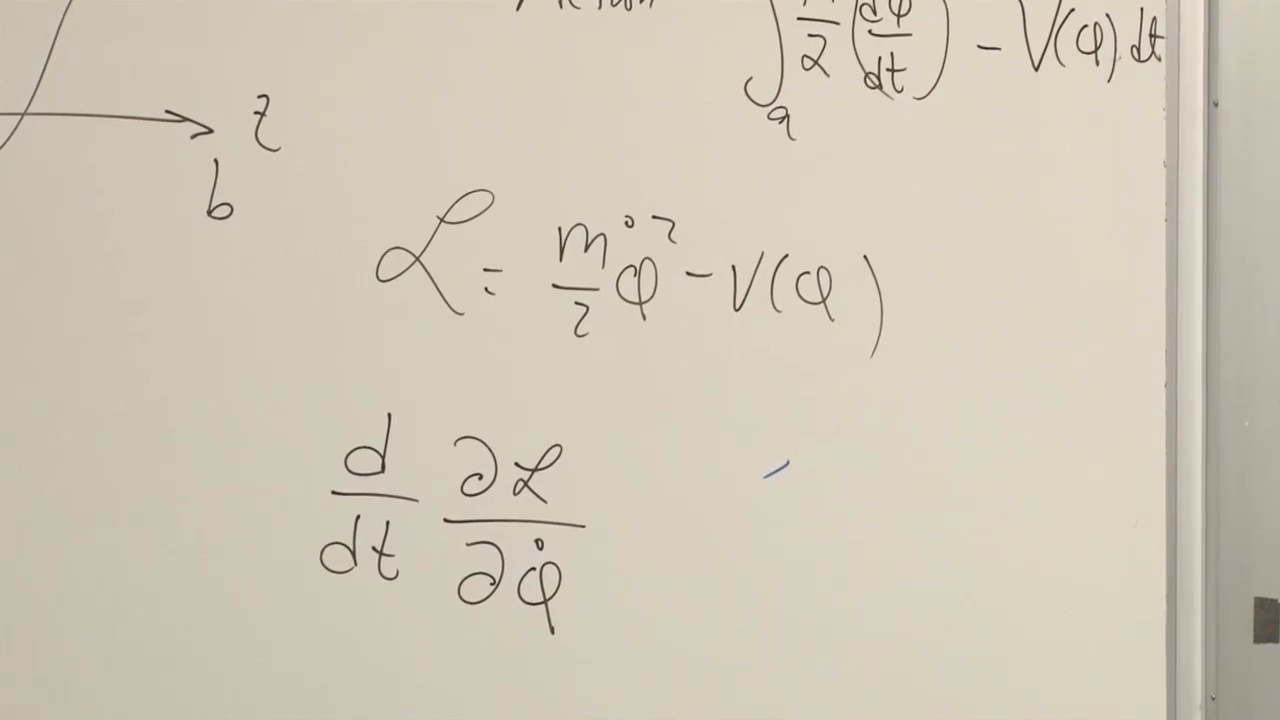
\includegraphics[width=0.90\textwidth]{lecture_04_figure_02.png}\caption{Die abgetastete Geschichte \(\phi(t)\): eine Teilchenbahn und, neu interpretiert, eine Feldgeschichte in \(0+1\) Dimensionen.}\lectureframe{00:14:30}\end{figure}

\begin{classroomqa}\audiencequestion{Verschwindet das Potential, wenn es keine räumlichen Dimensionen gibt?}\lecturerresponse{Nein. Die räumliche Variation verschwindet, aber das Feld hat weiterhin einen Wert. Die Energie kann von diesem Wert über \(V(\phi)\) abhängen. In der Teilchendeutung ändert eine Verschiebung der Kurve nach oben oder unten die potenzielle Energie; in der Felddarstellung tragen verschiedene Werte von \(\phi\) unterschiedliche potenzielle Energie. \lecturetimestamp{00:15:00}}\end{classroomqa}

\begin{classroomqa}\audiencequestion{Kann man sich statt eines Raums ohne Dimensionen auch einen gewöhnlichen Raum vorstellen, in dem das Feld nur von der Zeit abhängt?}\lecturerresponse{Ja. Für diesen Zweck ist die lokale Mathematik dieselbe: Alle räumlichen Ableitungen verschwinden, und nur \(\phi(t)\) bleibt. Die Bezeichnung als Theorie in \(0+1\) Dimensionen hebt diese reduzierte Struktur hervor, aber auch ein räumlich homogenes Feld in einer Welt mit mehr Dimensionen vermittelt dieselbe Anschauung. \lecturetimestamp{00:16:25}}\end{classroomqa}

Der Sinn dieses Umwegs ist nun klar. Wir kennen das Wirkungsprinzip für ein Feld, das von einer Koordinate, der Zeit, abhängt. Das daraus erkennbare Muster können wir nutzen, um das Wirkungsprinzip für ein Feld zu erschließen, das von allen Raumzeitkoordinaten abhängt.

\section{Eine Feldgeschichte über der Raumzeit}

\subsection{Von der Kurve zur Fläche}

In \(1+1\) Dimensionen ist die Raumzeit selbst eine Ebene mit den Koordinaten \(t\) und \(x\). Der Wert \(\phi(x,t)\) liefert eine dritte Richtung. Die Geschichte des Feldes ist daher keine Kurve, sondern eine Fläche über der Raumzeitebene. Die Fläche kann über null ansteigen oder darunter fallen, denn ein Skalarfeld muss nicht positiv sein.

\begin{figure}[htbp]\centering
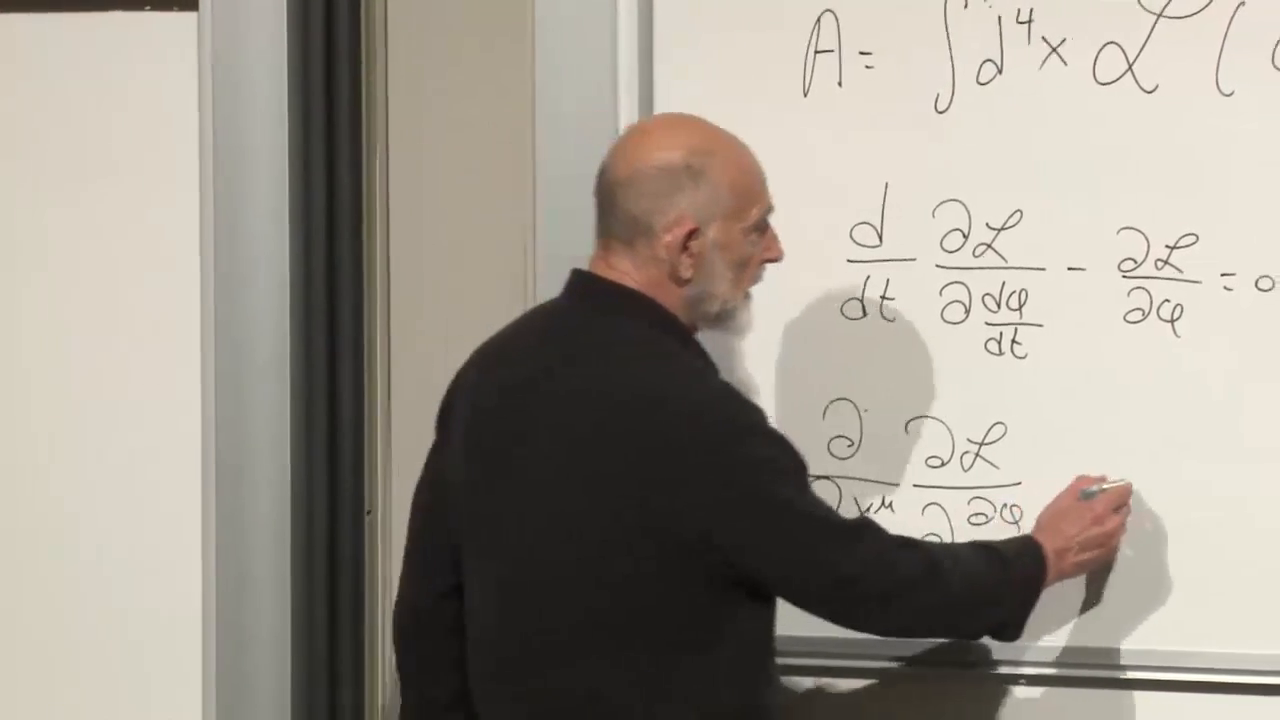
\includegraphics[width=0.90\textwidth]{lecture_04_figure_03.png}\caption{Eine Skalarfeldgeschichte, dargestellt als Fläche über einer Raumzeitebene mit \(1+1\) Dimensionen.}\lectureframe{00:20:46}\end{figure}

Unsere physikalische Raumzeit heißt \(3+1\)-dimensional: Sie hat drei Raumdimensionen und eine Zeitdimension. Ein Modell auf einer Tischplatte ist \(2+1\)-dimensional, und Perlen auf einem Draht veranschaulichen eine Welt mit \(1+1\) Dimensionen. Die zusätzliche Achse, die zur Darstellung von \(\phi\) nötig ist, macht selbst den Fall \(3+1\) unmöglich originalgetreu zeichnbar. Die Definition ist jedoch eindeutig: Eine vollständige Geschichte ordnet jedem Raumzeitereignis einen Wert von \(\phi\) zu.

\subsection{Von festen Endpunkten zu festen Randdaten}

Beim Variationsproblem für ein Teilchen werden zwei Endpunkte festgehalten und die Kurve dazwischen variiert. Das Analogon in der Feldtheorie wählt ein Raumzeitgebiet aus, hält \(\phi\) auf dessen Rand fest und variiert \(\phi\) im Inneren. Das Gebiet kann in einer Zeichnung mit \(1+1\) Dimensionen ein Rechteck sein oder in einer Raumzeit höherer Dimension ein beliebiges geeignetes Gebiet.

\begin{figure}[htbp]\centering
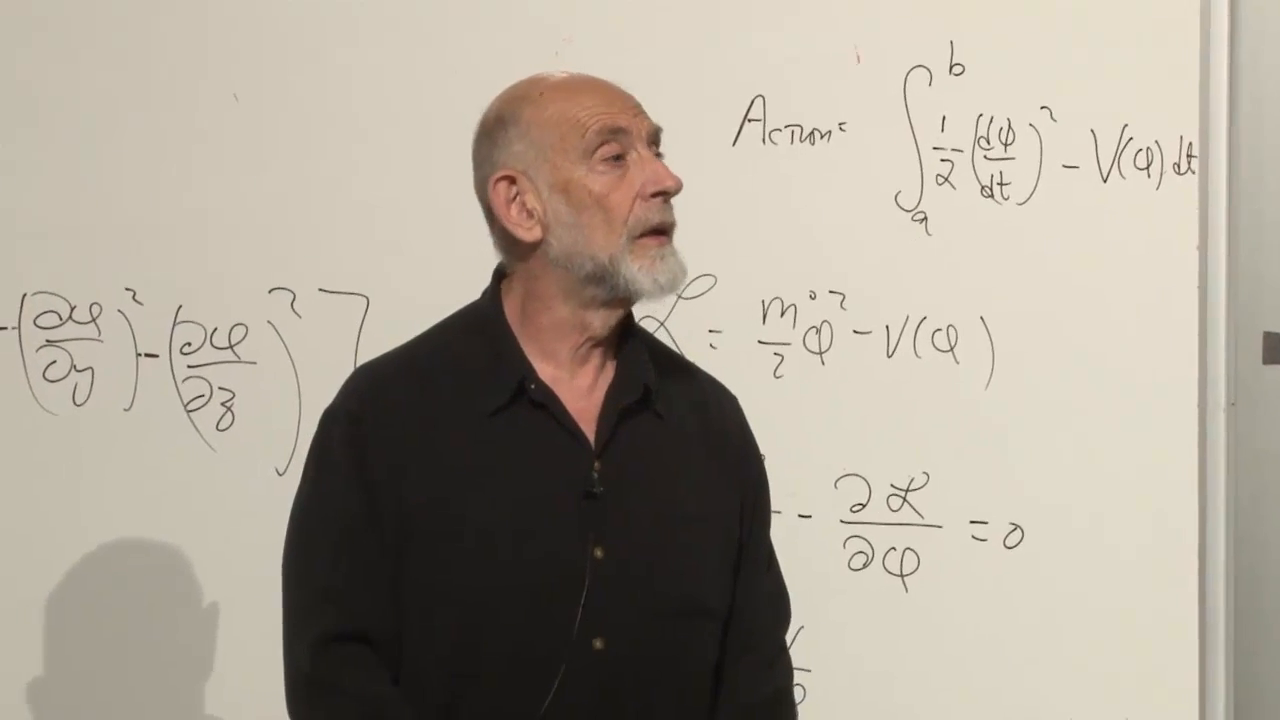
\includegraphics[width=0.90\textwidth]{lecture_04_figure_04.png}\caption{Ein Raumzeitgebiet, dessen gesamter Rand festgehalten wird, während das Feld im Inneren variiert wird.}\lectureframe{00:24:52}\end{figure}

\begin{classroomqa}\audiencequestion{Funktioniert die Lagrange-Formulierung auch dann, wenn ein Potential explizit von der Zeit abhängt?}\lecturerresponse{Ja. Die Euler--Lagrange- und die Hamilton-Formulierung funktionieren weiterhin. Im Allgemeinen geht jedoch die Energieerhaltung verloren: Explizite Zeitabhängigkeit bricht die Zeittranslationssymmetrie. In der Feldtheorie ist die entsprechende Aussage, dass eine explizite Raumzeitabhängigkeit zulässig ist, obwohl sie die zugehörigen Erhaltungssätze beeinflusst. \lecturetimestamp{00:23:49}}\end{classroomqa}

\begin{classroomqa}\audiencequestion{Wird beim rechteckigen Feldgebiet nur der obere und der untere Rand festgehalten oder der ganze Rand?}\lecturerresponse{Bei dieser Variationskonstruktion wird der ganze Rand festgehalten: alle vier Seiten des Rechtecks mit \(1+1\) Dimensionen. Das Feld darf nur im Inneren variieren. Dies ist das direkte Analogon dazu, beide Endpunkte in der Teilchenmechanik festzuhalten. \lecturetimestamp{00:24:24}}\end{classroomqa}

Den gesamten Rand festzuhalten ist eine Festlegung für die Variation, mit der die Gleichungen hergeleitet werden. Behandelt man die resultierende hyperbolische Feldgleichung als physikalisches Evolutionsproblem, gibt man üblicherweise geeignete Anfangsdaten vor und lässt die Gleichung sie in die Zukunft fortentwickeln.

\section{Die Wirkung und die Euler--Lagrange-Gleichung des Feldes}

\subsection{Die Lagrange-Dichte}

Zerlegen wir das Raumzeitgebiet in kleine Zellen. Es wird angenommen, dass sich die Wirkung aus lokalen Beiträgen zusammensetzt, je einem pro Zelle. Im Kontinuumslimes wird diese Summe zu einem Integral über die Raumzeit: \begin{equation}
A[\phi]
=
\int_{\Omega} d^4x\,
\mathcal{L}\!\left(
\phi,\partial_\mu\phi;x^\mu
\right),
\qquad
d^4x=dt\,dx\,dy\,dz.
\label{eq:sr4-field-action}
\end{equation} Die Größe \(\mathcal{L}\) ist die Lagrange-Dichte. Das Semikolon in \(\mathcal{L}(\phi,\partial_\mu\phi;x^\mu)\) trennt die dynamischen Argumente von einer möglichen expliziten Koordinatenabhängigkeit. In einem homogenen abgeschlossenen System fehlt diese letztere Abhängigkeit normalerweise, doch die Variationsformulierung schließt sie nicht aus.

Die kompakte Schreibweise \begin{equation}
\partial_\mu\phi
\equiv
\frac{\partial\phi}{\partial x^\mu}
\end{equation} fasst die Zeit- und Ortsableitungen zusammen. In der Komponentennotation der Vorlesung kann man stattdessen schreiben \begin{equation}
\begin{aligned}
\phi_t&=\frac{\partial\phi}{\partial t},\\
\phi_x&=\frac{\partial\phi}{\partial x},\\
\phi_y&=\frac{\partial\phi}{\partial y},\\
\phi_z&=\frac{\partial\phi}{\partial z}.
\end{aligned}
\label{eq:sr4-component-derivatives}
\end{equation} Es kann mehrere Felder geben, ebenso wie ein Teilchen mehrere Koordinaten haben kann. Vorerst gibt es nur ein Feld, \(\phi\).

Das Symbol \(d^4x\) ist lediglich eine Kurzschreibweise für das Maß über vier Koordinaten. In einer Raumzeit anderer Dimension würde es durch \(d^Dx\) ersetzt. Im Prototyp mit \(0+1\) Dimensionen gilt \(D=1\), und \(d^1x\) ist einfach \(dt\).

\begin{figure}[htbp]\centering
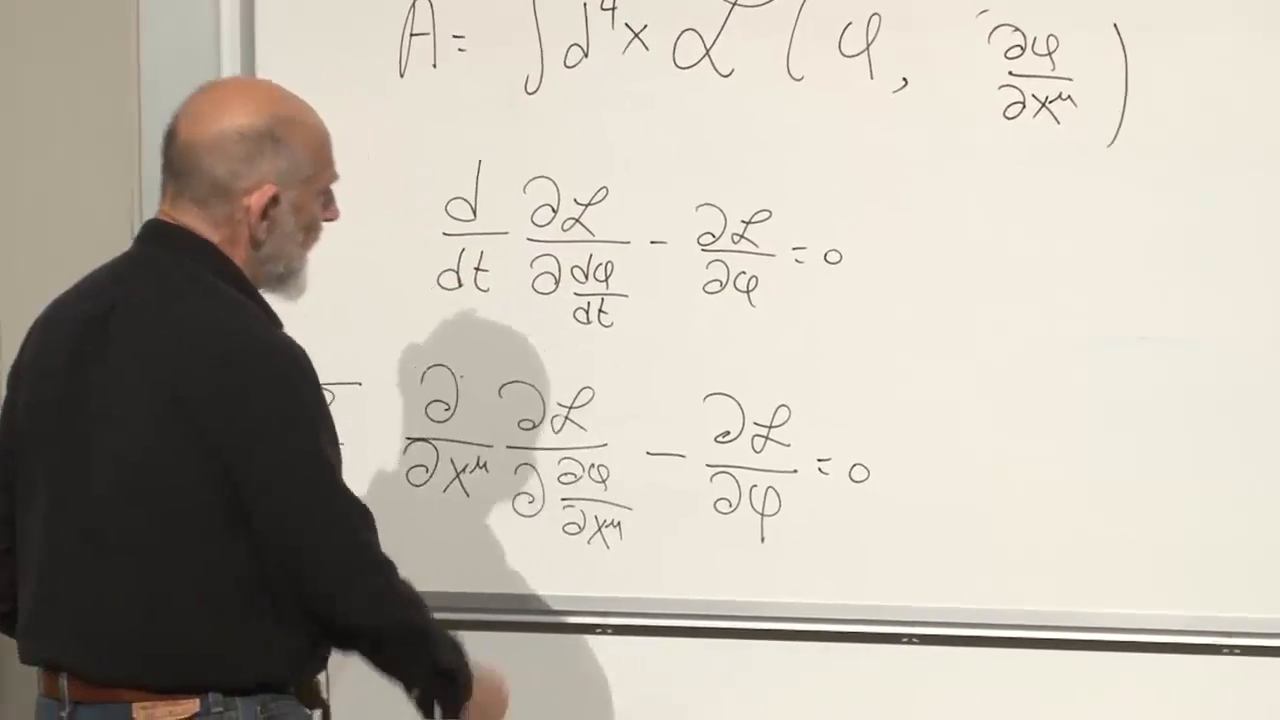
\includegraphics[width=0.90\textwidth]{lecture_04_figure_05.png}\caption{Die Wirkungsdichte als lokale Funktion von \(\phi\) und seinen Raumzeit-Ableitungen.}\lectureframe{00:32:51}\end{figure}

\begin{classroomqa}\audiencequestion{Kann die Lagrange-Dichte auch von \(x,y,z\) selbst abhängen?}\lecturerresponse{Das ist möglich, ebenso wie eine Teilchen-Lagrange-Funktion explizit von \(t\) abhängen kann. Bei einem translationsinvarianten abgeschlossenen System ist das üblicherweise nicht der Fall, aber eine explizite Koordinatenabhängigkeit macht die Formulierung nicht ungültig. \lecturetimestamp{00:30:29}}\end{classroomqa}

\begin{classroomqa}\audiencequestion{Gilt die bisherige Konstruktion speziell für ein Skalarfeld oder ist sie allgemein?}\lecturerresponse{Das Variationsschema ist bisher allgemein. Dass nur eine Komponente geschrieben wird, deutet auf ein Skalarfeld hin. Ein Vektorfeld oder eine Sammlung von Feldern hätte zusätzliche Komponentenindizes, und jede Komponente würde variiert. \lecturetimestamp{00:31:00}}\end{classroomqa}

\subsection{Das Gitterbild}

Auf einem feinen Raumzeitgitter werden Ableitungen zu Differenzen zwischen benachbarten Feldwerten. Die Wirkung ist dann eine gewöhnliche Funktion vieler Variablen. Ein Gitter mit zehn Punkten in der einen und acht in der anderen Richtung hat bereits achtzig Feldvariablen. Bei einer Verfeinerung des Gitters nimmt ihre Zahl zu, aber die Minimierungsregel bleibt einfach: Man leitet die Wirkung nach dem Feldwert an jedem inneren Punkt ab und setzt das Ergebnis gleich null.

\begin{figure}[htbp]\centering
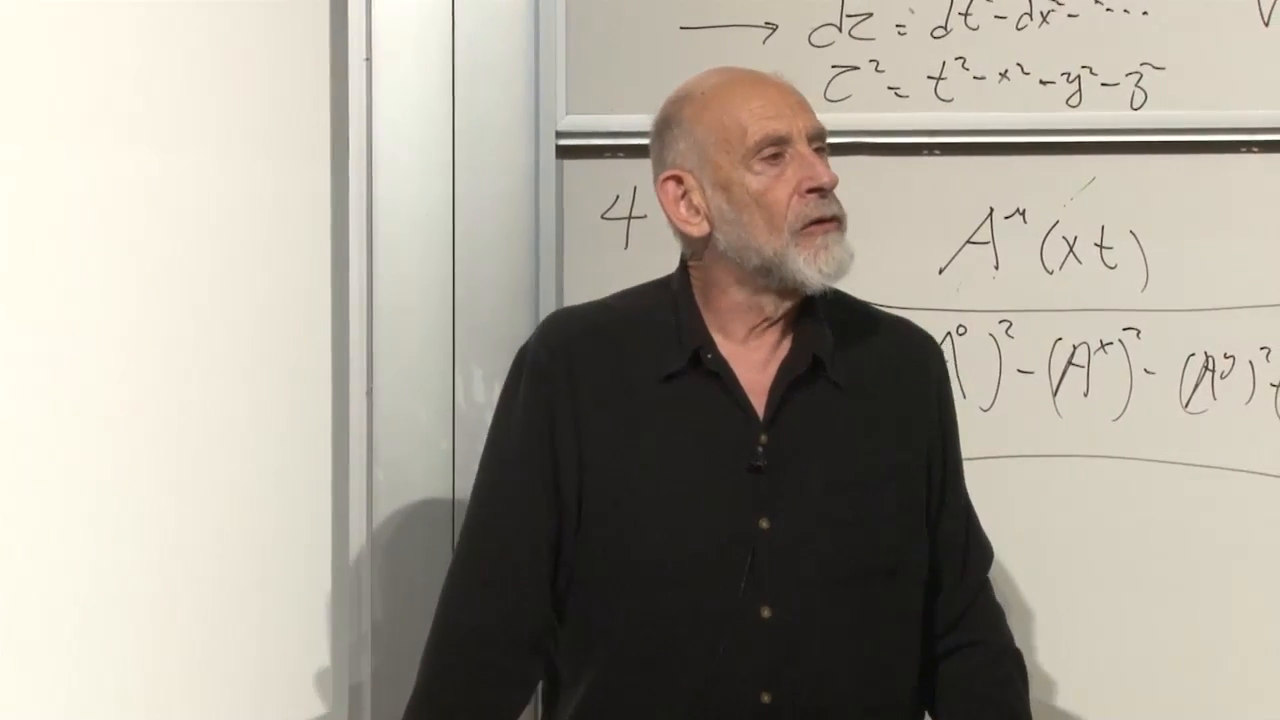
\includegraphics[width=0.90\textwidth]{lecture_04_figure_06.png}\caption{Das in Zellen unterteilte Raumzeitgebiet: Vor dem Kontinuumslimes wird die Wirkung so zu einer gewöhnlichen Funktion vieler Variablen.}\lectureframe{00:34:05}\end{figure}

Im Kontinuumslimes erhält man die Euler--Lagrange-Gleichung des Feldes, \begin{equation}
\boxed{
\partial_\mu
\left[
\frac{\partial\mathcal{L}}
{\partial(\partial_\mu\phi)}
\right]
-
\frac{\partial\mathcal{L}}{\partial\phi}
=0
}.
\label{eq:sr4-field-el}
\end{equation} Über den wiederholten Index \(\mu\) wird über alle Raumzeitrichtungen summiert. Ohne diese Summationskonvention lautet dieselbe Gleichung \begin{align}
&
\frac{\partial}{\partial t}
\left(\frac{\partial\mathcal{L}}{\partial\phi_t}\right)
+
\frac{\partial}{\partial x}
\left(\frac{\partial\mathcal{L}}{\partial\phi_x}\right)
+
\frac{\partial}{\partial y}
\left(\frac{\partial\mathcal{L}}{\partial\phi_y}\right)
\nonumber\\
&\hspace{3em}
+
\frac{\partial}{\partial z}
\left(\frac{\partial\mathcal{L}}{\partial\phi_z}\right)
-
\frac{\partial\mathcal{L}}{\partial\phi}
=0.
\label{eq:sr4-field-el-expanded}
\end{align} Der erste Term ist aus der Teilchenmechanik vertraut. Die Feldtheorie ergänzt einen analogen Term für jede räumliche Richtung. Der letzte Term, \(-\partial\mathcal{L}/\partial\phi\), bleibt unverändert.

\begin{figure}[htbp]\centering
\includegraphics[width=0.90\textwidth]{lecture_04_figure_07.png}\caption{Die eindimensionale Euler--Lagrange-Gleichung und ihre Raumzeitverallgemeinerung, untereinander dargestellt.}\lectureframe{00:38:44}\end{figure}

Dieses Gebiet wird auch Kontinuumsmechanik genannt. Je nach den Freiheitsgraden kann dieselbe Mathematik Strömungen, elastische Verformungen oder ein anderes kontinuierliches Medium beschreiben.

\begin{classroomqa}\audiencequestion{Würden dieselben Gleichungen in einer Welt mit Raum, aber ohne Zeit funktionieren?}\lecturerresponse{Ja, als rein räumliches Variationsproblem. Physikalisch sucht man so nach einer statischen Lösung: Man nimmt an, dass das Feld zeitunabhängig ist, verwirft alle Zeitableitungen und löst die verbleibenden räumlichen Gleichungen. Eine zeitunabhängige elektrische oder magnetische Konfiguration ist ein Beispiel. \lecturetimestamp{00:40:05}}\end{classroomqa}

\section{Die einfachste Skalarfelddynamik erschließen}

\subsection{Warum die Vorzeichen nicht alle gleich sein können}

Kehren wir zum kinetischen Term des Teilchens \(\tfrac12\dot\phi^2\) zurück, setzen wir seinen irrelevanten Gesamtfaktor auf eins und versuchen wir, ihn zu verallgemeinern. Ein erster Ansatz könnte \begin{equation}
\mathcal{L}_{+}
=
\frac12
\left[
\phi_t^2+\phi_x^2+\phi_y^2+\phi_z^2
\right].
\label{eq:sr4-all-plus}
\end{equation} sein. Das ist ein nützlicher Irrweg. Er behandelt Zeit und Raum mit gleichen Vorzeichen. Die resultierende Gleichung hätte nicht die hyperbolische Struktur der Wellenausbreitung. Die korrekte relativistische Kombination hat für die Zeit ein Vorzeichen und für den Raum das entgegengesetzte.

\begin{classroomqa}\audiencequestion{Ist der Ausdruck mit ausschließlich positiven Vorzeichen falsch, weil die Lagrange-Funktion relativistisch invariant sein muss?}\lecturerresponse{Das ist die grundlegendere Antwort, und sie ist richtig. Die Vorlesung gelangt zunächst auf anschaulichere Weise zu den Vorzeichen: Wellen unterscheiden die zeitliche Entwicklung von der räumlichen Variation, daher darf die Zeit nicht genau wie eine weitere räumliche Koordinate eingehen. Die Lorentz-Invarianz wird diese Anschauung gleich in eine präzise Regel überführen. \lecturetimestamp{00:43:19}}\end{classroomqa}

Stellen wir eine charakteristische Geschwindigkeit \(c\) wieder her, so lautet die einfache Lagrange-Dichte des Skalarfeldes \begin{equation}
\boxed{
\mathcal{L}
=
\frac12
\left[
\frac{1}{c^2}\phi_t^2
-\phi_x^2-\phi_y^2-\phi_z^2
\right]
-V(\phi)
}.
\label{eq:sr4-scalar-lagrangian}
\end{equation} Für ein relativistisches Feld ist \(c\) die Lichtgeschwindigkeit. In einem Kontinuumsmodell könnte es stattdessen die Schallgeschwindigkeit, die Geschwindigkeit einer elastischen Welle oder eine andere charakteristische Ausbreitungsgeschwindigkeit sein.

Der Gesamtfaktor \(1/2\) ist Konvention, genauso wie bei \(\tfrac12m\dot\phi^2\). Multipliziert man eine gesamte Wirkung mit einer von null verschiedenen Konstanten, ändern sich ihre stationären Pfade nicht; die Konvention legt fest, wie die Parameter in den Gleichungen benannt und normiert werden. Ist diese Normierung einmal gewählt, muss sie konsequent verwendet werden.

\begin{classroomqa}\audiencequestion{Kann man die Terme mit räumlichen Gradienten als Teil der potenziellen Energie auffassen?}\lecturerresponse{Ja. Bei der Aufteilung in kinetische minus potenzielle Energie enthält der kinetische Anteil Zeitableitungen. Terme ohne Zeitableitungen, darunter räumliche Gradienten und \(V(\phi)\), gehören zum Anteil der potenziellen Energie. Der letztliche Grund für ihre relativen Vorzeichen in einer relativistischen Theorie ist die Lorentz-Metrik. \lecturetimestamp{00:45:37}}\end{classroomqa}

\subsection{Die Wellengleichung}

Wenden wir \eqref{eq:sr4-field-el} an. Für die Ableitungsterme gilt \begin{equation}
\frac{\partial\mathcal{L}}{\partial\phi_t}
=\frac{1}{c^2}\phi_t,
\qquad
\frac{\partial\mathcal{L}}{\partial\phi_i}
=-\phi_i,
\end{equation} während \begin{equation}
\frac{\partial\mathcal{L}}{\partial\phi}
=-\frac{dV}{d\phi}.
\end{equation} Damit folgt \begin{equation}
\begin{aligned}
&\boxed{
\frac{1}{c^2}\frac{\partial^2\phi}{\partial t^2}
-\nabla^2\phi
+\frac{dV}{d\phi}
=0
},\\[0.5em]
\nabla^2
&=
\frac{\partial^2}{\partial x^2}
+\frac{\partial^2}{\partial y^2}\\
&\quad
+\frac{\partial^2}{\partial z^2}.
\end{aligned}
\label{eq:sr4-general-scalar-eom}
\end{equation}

Für \(V=0\) vereinfacht sich dies zu \begin{equation}
\boxed{
\frac{1}{c^2}\phi_{tt}-\nabla^2\phi=0
},
\label{eq:sr4-wave-equation}
\end{equation} der Wellengleichung. Die Vorlesung erkennt die Gleichung, verschiebt ihre Lösung aber auf später. Ihre Lösungen breiten Störungen mit der Geschwindigkeit \(c\) aus.

\begin{figure}[htbp]\centering
\includegraphics[width=0.90\textwidth]{lecture_04_figure_08.png}\caption{Die eindimensionale Form \(c^{-2}\phi_{tt}-\phi_{xx}=0\), erkannt als Wellengleichung.}\lectureframe{00:50:30}\end{figure}

\subsection{Ein Feld gekoppelter harmonischer Oszillatoren}

Wählen wir nun ein quadratisches Potential, \begin{equation}
V(\phi)=\frac12\mu^2\phi^2,
\qquad
\frac{dV}{d\phi}=\mu^2\phi.
\label{eq:sr4-quadratic-potential}
\end{equation} Wäre \(\phi\) die Position eines Teilchens, so wäre dies das Potential eines harmonischen Oszillators mit der Federkonstante \(\mu^2\). Für das Feld gilt \begin{equation}
\boxed{
\frac{1}{c^2}\phi_{tt}-\nabla^2\phi+\mu^2\phi=0
}.
\label{eq:sr4-klein-gordon}
\end{equation} Ohne die räumliche Ableitung ist dies einfach eine Beschleunigung plus eine Konstante mal Auslenkung, gleich null. Der Gradient koppelt benachbarte Punkte und macht aus dem Oszillator ein wellentragendes Kontinuum. In der relativistischen Feldtheorie heißt \eqref{eq:sr4-klein-gordon} massive Klein--Gordon-Gleichung; klassisch ist \(\mu\) die inverse Längenskala, die die Wellenausbreitung verändert.

\begin{figure}[htbp]\centering
\includegraphics[width=0.90\textwidth]{lecture_04_figure_09.png}\caption{Das quadratische Potential und die daraus folgende Wellengleichung mit dem Rückstellterm \(\mu^2\phi\).}\lectureframe{00:52:38}\end{figure}

\begin{classroomqa}\audiencequestion{Warum verschwindet der Faktor \(1/2\) in \(V=\tfrac12\mu^2\phi^2\) aus der Bewegungsgleichung?}\lecturerresponse{Beim Ableiten von \(\phi^2\) entsteht ein Faktor zwei. Der konventionelle Faktor \(1/2\) wird genau deshalb eingeführt, damit \(dV/d\phi=\mu^2\phi\) gilt, so wie \(V(x)=\tfrac12kx^2\) die Rückstellkraft \(-kx\) ergibt. \lecturetimestamp{00:53:17}}\end{classroomqa}

Die Gleichung ist linear: \(\phi\) und jede seiner Ableitungen treten nur in erster Potenz auf. Terme wie \(\phi^2\) oder \(\phi\,\partial_\mu\phi\) in der Bewegungsgleichung würden die Dynamik nichtlinear machen.

\section{Lorentz-Skalare und Vierervektoren}

\subsection{Die Wirkung muss bezugssystemunabhängig sein}

Die Variationsmethodik allein legt viele mögliche Feldtheorien fest. Die Relativitätstheorie stellt zusätzlich die Forderung, dass die Wirkung in jedem Inertialsystem denselben Wert und dieselbe Form hat. Beim freien Teilchen wurde dies erreicht, indem man die invariante Eigenzeit \(d\tau\) entlang der Weltlinie integrierte. Bei einem Feld wird die Wirkung über die Raumzeit integriert; daher müssen sich ihre lokalen Bausteine in geeigneter Weise transformieren.

Unter einer eigentlichen Lorentz-Transformation ist das Raumzeitmaß invariant, \(d^4x'=d^4x\). Daher genügt es, von der Lagrange-Dichte zu verlangen, dass sie ein Lorentz-Skalar ist: \begin{equation}
\mathcal{L}'(x')=\mathcal{L}(x).
\label{eq:sr4-lagrangian-scalar}
\end{equation}

\subsection{Skalarfelder}

Ein Skalarfeld erfüllt \begin{equation}
\boxed{\phi'(x')=\phi(x)}.
\label{eq:sr4-scalar-transform}
\end{equation} Die Koordinaten \(x\) und \(x'\) bezeichnen dasselbe Ereignis in zwei Bezugssystemen. Die von den Beobachtern verwendeten Funktionsterme können unterschiedlich aussehen, aber der diesem physikalischen Ereignis zugeordnete Zahlenwert ist derselbe.

\begin{figure}[htbp]\centering
\includegraphics[width=0.90\textwidth]{lecture_04_figure_10.png}\caption{Das definierende Transformationsgesetz eines Skalarfeldes: \(\phi(x)=\phi'(x')\).}\lectureframe{00:59:33}\end{figure}

Die Temperatur lieferte die erste Anschauung, auch wenn ein bewegtes Thermometer in einem materiellen Medium kein vollkommenes relativistisches Beispiel ist. Entscheidend ist die Definition \eqref{eq:sr4-scalar-transform}, nicht die Analogie mit dem Thermometer.

\subsection{Vierervektoren}

In Einheiten \(c=1\) wirkt ein Boost mit der Geschwindigkeit \(v\) entlang der \(x\)-Achse wie folgt: \begin{equation}
\begin{aligned}
t'&=\gamma(t-vx),\\
x'&=\gamma(x-vt),\\
y'&=y,\\
z'&=z,\\
\gamma&=\frac{1}{\sqrt{1-v^2}}.
\end{aligned}
\label{eq:sr4-x-boost}
\end{equation}

\begin{figure}[htbp]\centering
\includegraphics[width=0.90\textwidth]{lecture_04_figure_11.png}\caption{Die Lorentz-Transformation für einen Boost entlang der \(x\)-Achse in Einheiten \(c=1\).}\lectureframe{01:02:26}\end{figure}

Vier Größen, die sich unter Boosts auf dieselbe Weise mischen, bilden einen Vierervektor. Beispiele, denen wir bereits begegnet sind, sind \(x^\mu\), \(dx^\mu\) und die Vierergeschwindigkeit \(u^\mu=dx^\mu/d\tau\). Das Produkt eines Vierervektors mit einem Skalar ergibt wieder einen Vierervektor. Eine strömende relativistische Flüssigkeit liefert ein feldwertiges Beispiel: Ihre Vierergeschwindigkeit \(u^\mu(x)\) kann sich von Ereignis zu Ereignis unterscheiden.

Für denselben Boost wie in \eqref{eq:sr4-x-boost} erfüllt ein allgemeiner Vierervektor \begin{equation}
\begin{aligned}
A'^0&=\gamma(A^0-vA^x),\\
A'^x&=\gamma(A^x-vA^0),\\
A'^y&=A^y,\\
A'^z&=A^z.
\end{aligned}
\label{eq:sr4-vector-boost}
\end{equation}

Für einen allgemeinen Vierervektor \(A^\mu=(A^0,A^x,A^y,A^z)\) ist die Lorentzsche Norm \begin{equation}
\boxed{
A_\mu A^\mu
=(A^0)^2-(A^x)^2-(A^y)^2-(A^z)^2
}
\label{eq:sr4-vector-norm}
\end{equation} ein Skalar. Sie ist aus demselben algebraischen Grund invariant wie \begin{equation}
d\tau^2=dt^2-dx^2-dy^2-dz^2
\end{equation}. Der Vorlesung gehen kurz die unverbrauchten Buchstaben für einen allgemeinen Vektor aus, bevor sie \(A\) akzeptiert, angeregt durch den Vorschlag \(A\) als Abkürzung für „arrow“ zu verwenden.

\begin{figure}[htbp]\centering
\includegraphics[width=0.90\textwidth]{lecture_04_figure_12.png}\caption{Ein allgemeines Vierervektorfeld und die Lorentzsche Differenz der Quadrate, aus der seine invariante Norm gebildet wird.}\lectureframe{01:09:06}\end{figure}

\subsection{Die Ableitung eines Skalarfeldes}

Die Ableitung eines Skalarfeldes nach den vier Raumzeitkoordinaten ergibt die vier Komponenten \begin{equation}
\partial_\mu\phi
=
\left(
\frac{\partial\phi}{\partial t},
\frac{\partial\phi}{\partial x},
\frac{\partial\phi}{\partial y},
\frac{\partial\phi}{\partial z}
\right)
\qquad(c=1).
\end{equation} Streng genommen ist \(\partial_\mu\phi\) eine Kovektorkomponente; durch Anheben des Index mit der Minkowski-Metrik erhält man \(\partial^\mu\phi\). Für das Komponentenargument hier ist dieser Unterschied unerheblich, doch er legt die Kontraktion eindeutig fest: \begin{equation}
\boxed{
\partial_\mu\phi\,\partial^\mu\phi
=
\frac{1}{c^2}\phi_t^2
-\phi_x^2-\phi_y^2-\phi_z^2
}.
\label{eq:sr4-derivative-scalar}
\end{equation}

\begin{figure}[htbp]\centering
\includegraphics[width=0.90\textwidth]{lecture_04_figure_13.png}\caption{Die invariante Differenz der Quadrate aus den ersten Ableitungen eines Skalarfeldes.}\lectureframe{01:13:55}\end{figure}

\begin{classroomqa}\audiencequestion{Ist diese Kombination von Ableitungen der Laplace-Operator?}\lecturerresponse{Nein. Die dargestellte invariante Größe ist quadratisch in den ersten Ableitungen. Der Laplace-Operator enthält zweite räumliche Ableitungen. Zweite Ableitungen treten erst nach der Variation der Wirkung in der Wellengleichung auf. \lecturetimestamp{01:13:22}}\end{classroomqa}

Das Vorzeichenmuster in \eqref{eq:sr4-scalar-lagrangian} lässt sich jetzt erklären, statt es nur zu erraten. Die Kombination aus kinetischem Term und Gradient ist der Lorentz-Skalar \(\partial_\mu\phi\,\partial^\mu\phi\). Damit lautet die einfachste quadratische Theorie \begin{equation}
\mathcal{L}
=
\frac12\partial_\mu\phi\,\partial^\mu\phi
-\frac12\mu^2\phi^2.
\label{eq:sr4-covariant-lagrangian}
\end{equation}

\begin{figure}[htbp]\centering
\includegraphics[width=0.90\textwidth]{lecture_04_figure_14.png}\caption{Die vervollständigte quadratische Lagrange-Dichte des Skalarfeldes und ihre lineare Feldgleichung an der Tafel.}\lectureframe{01:19:12}\end{figure}

\section{Wie viel Freiheit gibt es?}

Sobald die Regel zur Bildung von Skalaren bekannt ist, sind viele Lagrange-Dichten möglich. Das Feld \(\phi\) ist ein Skalar, also ist auch jede gewöhnliche Funktion \(F(\phi)\) ein Skalar: \(\phi^2\), \(\phi^3\), \(\cosh\phi\) und so weiter. Auch numerische Parameter sind zulässig. Ein Symbol wie \(\mu\) kann als konstanter Koeffizient eingesetzt werden; offen bleiben nur seine Dimensionen und seine physikalische Deutung.

\begin{classroomqa}\audiencequestion{Kann man eine Masse in die Lagrange-Dichte aufnehmen?}\lecturerresponse{Ein konstanter Parameter ist gewiss zulässig. An dieser Stelle sollte man fragen, um die Masse welchen Objekts es sich handelt, denn \(\mu\) ist in der klassischen Feldtheorie zunächst einfach eine Zahl, bis ihre physikalische Bedeutung bestimmt ist. In der quadratischen relativistischen Skalarfeldtheorie legt sie die Masse oder die inverse Längenskala fest. \lecturetimestamp{01:14:16}}\end{classroomqa}

Skalare lassen sich miteinander multiplizieren: \begin{equation}
F(\phi)\,\partial_\mu\phi\,\partial^\mu\phi
\end{equation} ist Lorentz-invariant. Auch der Ableitungsskalar selbst kann quadriert werden, wodurch höhere Potenzen erster Ableitungen entstehen. Ebenso kann man höhere Ableitungen in Betracht ziehen, doch die Vorlesung beschränkt sich auf Felder und ihre ersten Ableitungen, den üblichen Rahmen, der Bewegungsgleichungen zweiter Ordnung liefert. Bei Theorien mit höheren Ableitungen ist zusätzliche Sorgfalt nötig, weil sie im Allgemeinen weitere dynamische Daten und mögliche Instabilitäten mit sich bringen.

\begin{classroomqa}\audiencequestion{Ist die Konstruktion als Differenz von Quadraten tatsächlich die Metrik der Raumzeit?}\lecturerresponse{Ja. In der gewählten Signatur lautet die Metrik \(dt^2-dx^2-dy^2-dz^2\). Das Wort „Metrik“ wurde in der Vorlesung bisher nicht hervorgehoben, aber genau diese Raumzeitgeometrie wird in der allgemeinen Relativitätstheorie zentral werden. \lecturetimestamp{01:19:39}}\end{classroomqa}

\begin{classroomqa}\audiencequestion{Gibt es allgemeinere Objekte als Vierervektoren mit Komponenten wie \(xy\) oder \(tx\)?}\lecturerresponse{Ja. Das sind Tensoren. Ein Skalar hat keinen Raumzeitindex, ein Vektor einen und ein Tensor zweiten Ranges Komponenten wie \(T^{xx}\), \(T^{xy}\) und \(T^{tx}\). Der größte Teil der bisherigen Diskussion über Skalarfelder kommt ohne sie aus; in der allgemeinen Relativitätstheorie sind sie unverzichtbar. \lecturetimestamp{01:20:49}}\end{classroomqa}

\begin{classroomqa}\audiencequestion{Warum betrachtet man nur Boosts, die \(t\) mit \(x\) mischen? Könnte ein Boost in eine andere Richtung zeigen und die Raumachsen anders mischen?}\lecturerresponse{Durchaus. Ein Boost entlang \(y\) mischt \(t\) mit \(y\) und lässt \(x,z\) unverändert. Eine allgemeine Lorentz-Transformation lässt sich aus räumlichen Drehungen und einem Boost entlang einer gewählten Achse zusammensetzen. Es genügt daher, die Rotationsinvarianz und die Invarianz unter einem Boost entlang einer Standardachse nachzuweisen. \lecturetimestamp{01:22:06}}\end{classroomqa}

\begin{classroomqa}\audiencequestion{Beschreiben alle Lagrange-Dichten, die sich aus so vielen möglichen Skalarmischungen ergeben, sinnvolle Physik?}\lecturerresponse{Auf klassischer Ebene ist die Freiheit enorm, sofern zusätzliche Anforderungen wie sinnvolle Vorzeichen, Lokalität und ein wohldefiniertes Evolutionsproblem erfüllt sind. Deutlich weniger willkürliche Wahlmöglichkeiten ergeben wohldefinierte fundamentale Quantentheorien. Die moderne effektive Feldtheorie lässt viele weitere Wechselwirkungen unterhalb einer Abschneideskala zu; dann muss jedoch der Gültigkeitsbereich angegeben werden. \lecturetimestamp{01:27:57}}\end{classroomqa}

\begin{classroomqa}\audiencequestion{Muss ein Feld stetig sein?}\lecturerresponse{Für die hier betrachteten glatten Theorien: ja. Ein Sprung führt zu singulären Ableitungen und bei einem quadratischen Gradiententerm typischerweise zu unendlicher Wirkung und Energie. Singulärere Konfigurationen lassen sich nur mit zusätzlicher mathematischer Struktur behandeln; sie sind nicht die gewöhnlichen Felder endlicher Energie, die hier entwickelt werden. \lecturetimestamp{01:29:29}}\end{classroomqa}

\section{Ein Teilchen in Kopplung an ein Skalarfeld}

\subsection{Das freie Teilchen erneut betrachtet}

Im letzten Teil der Vorlesung werden Teilchen und Felder auf klassischer Ebene zusammengeführt. Es geht noch nicht um die quantenmechanische Aussage, dass Teilchen Anregungen von Feldern sind. Nehmen wir stattdessen an, jemand habe bereits ein Hintergrund-Skalarfeld \(\phi(x,t)\) berechnet, und fragen wir, wie sich ein Teilchen darin bewegt.

Für ein freies relativistisches Teilchen gilt
\begin{equation}
A_{\rm free}=-m\int d\tau.
\label{eq:sr4-free-particle-action}
\end{equation}
In einer Raumdimension und bei \(c=1\) gilt
\begin{equation}
d\tau=dt\sqrt{1-\dot x^2},
\qquad
L_{\rm free}=-m\sqrt{1-\dot x^2}.
\label{eq:sr4-free-particle-l}
\end{equation}
Das Minuszeichen wird so gewählt, dass die Entwicklung für kleine Geschwindigkeiten den üblichen positiven Newtonschen kinetischen Term ergibt:
\begin{equation}
L_{\rm free}
\approx -m+\frac12m\dot x^2+\cdots.
\end{equation}

\begin{figure}[htbp]
\centering
\includegraphics[width=0.90\textwidth]{lecture_04_figure_15.png}
\caption{Die invariante Wirkung für ein freies Teilchen, umgeschrieben als Lagrange-Funktion bezüglich der Koordinatenzeit.}
\lectureframe{01:34:31}
\end{figure}

\subsection{Die einfachste skalare Kopplung}

Sowohl \(d\tau\) als auch \(\phi\) sind Skalare. Die einfachste lineare Kopplung lautet daher
\begin{equation}
\boxed{
A
=
\int d\tau\,[-m+\phi(x,t)]
}.
\label{eq:sr4-coupled-action}
\end{equation}
Diese Wahl ist nicht eindeutig. Man könnte \(\phi\) durch eine beliebige Funktion \(F(\phi)\) ersetzen. Der lineare Term genügt, um die physikalische Idee zu veranschaulichen.

\begin{figure}[htbp]
\centering
\includegraphics[width=0.90\textwidth]{lecture_04_figure_16.png}
\caption{Die freie Wirkung ergänzt um die einfachste Lorentz-invariante skalare Kopplung.}
\lectureframe{01:37:21}
\end{figure}

\begin{classroomqa}
\audiencequestion{Muss \(\phi\) innerhalb des Integrals bleiben?}
\lecturerresponse{Ja. Das Feld wird auf der Weltlinie des Teilchens ausgewertet, \(\phi(x(t),t)\), und ändert sich im Allgemeinen von einem Punkt der Bahn zum nächsten. Selbst wenn der Hintergrund keine explizite Zeitabhängigkeit aufweist, \(\phi=\phi(x)\), ändert er sich dennoch mit der Zeit, wenn sich das Teilchen durch den Raum bewegt. Nur ein entlang der Bahn konstantes Feld könnte vor das Integral gezogen werden. \lecturetimestamp{01:37:47}}
\end{classroomqa}

\begin{classroomqa}
\audiencequestion{Bedeutet das \(x\) in \(\phi(x,t)\) die Position des Teilchens?}
\lecturerresponse{Ja. Es ist \(x=x(t)\), die Position des Teilchens zum Zeitpunkt \(t\). Die Wirkung erfasst das vorgegebene Raumzeitfeld entlang dieser Bahn. \lecturetimestamp{01:38:08}}
\end{classroomqa}

Für eine eindimensionale Bewegung ergibt sich aus \eqref{eq:sr4-coupled-action}
\begin{equation}
L
=
-(m-\phi(x,t))\sqrt{1-\dot x^2}.
\label{eq:sr4-coupled-lagrangian}
\end{equation}
Das skalare Hintergrundfeld tritt genau an die Stelle der Ruhemasse:
\begin{equation}
m_{\rm eff}(x,t)=m-\phi(x,t).
\label{eq:sr4-effective-mass}
\end{equation}
Wenn sich \(\phi\) auf einen nahezu konstanten, von null verschiedenen Wert einpendelt, verhält sich das Teilchen, als hätte sich seine Masse geändert. Dies ist nur ein klassisches Spielzeugmodell und nicht der vollständige Higgs-Mechanismus, vermittelt aber einen Eindruck von der Grundidee des Higgs-Mechanismus: Ein skalarer Hintergrund kann als Massenterm in die Teilchendynamik eingehen.

\subsection{Die Teilchengleichung}

Der kanonische Impuls lautet
\begin{equation}
p
=
\frac{\partial L}{\partial\dot x}
=
(m-\phi)
\frac{\dot x}{\sqrt{1-\dot x^2}}.
\label{eq:sr4-coupled-momentum}
\end{equation}

\begin{figure}[htbp]
\centering
\includegraphics[width=0.90\textwidth]{lecture_04_figure_17.png}
\caption{Der skalare Hintergrund ersetzt \(m\) durch \(m-\phi(x,t)\) im relativistischen kanonischen Impuls.}
\lectureframe{01:43:38}
\end{figure}

Die Ortsableitung der Lagrange-Funktion lautet
\begin{equation}
\frac{\partial L}{\partial x}
=
\frac{\partial\phi}{\partial x}
\sqrt{1-\dot x^2}.
\end{equation}
Bei festgehaltenem Vorzeichen, das durch die Wirkung \eqref{eq:sr4-coupled-action} vorgegeben ist, lautet die Euler--Lagrange-Gleichung daher
\begin{equation}
\boxed{
\frac{d}{dt}
\left[
(m-\phi)
\frac{\dot x}{\sqrt{1-\dot x^2}}
\right]
=
\frac{\partial\phi}{\partial x}
\sqrt{1-\dot x^2}
}.
\label{eq:sr4-coupled-eom}
\end{equation}

\begin{figure}[htbp]
\centering
\includegraphics[width=0.90\textwidth]{lecture_04_figure_18.png}
\caption{Die gekoppelte Gleichung wird aus dem Impuls und der räumlichen Ableitung des Hintergrundfeldes zusammengesetzt; die Wirkung legt das endgültige Vorzeichen in \eqref{eq:sr4-coupled-eom} fest.}
\lectureframe{01:45:24}
\end{figure}

\begin{classroomqa}
\audiencequestion{Warum bleibt in \(\partial\phi/\partial x\) der Faktor \(\sqrt{1-\dot x^2}\) erhalten?}
\lecturerresponse{Weil nur der Faktor \(\phi(x,t)\) nach \(x\) abgeleitet wird. In der Lagrange-Funktion wird er mit der Quadratwurzel multipliziert, die bei festgehaltenem \(\dot x\) in der partiellen Ableitung nicht von der Position abhängt. Daher bleibt die Quadratwurzel erhalten. \lecturetimestamp{01:45:50}}
\end{classroomqa}

Durch Ausmultiplizieren der totalen Zeitableitung ergibt sich
\begin{align}
&(m-\phi)
\frac{d}{dt}
\left(
\frac{\dot x}{\sqrt{1-\dot x^2}}
\right)
-
\dot\phi\,
\frac{\dot x}{\sqrt{1-\dot x^2}}
\nonumber\\
&\hspace{10em}
=
\frac{\partial\phi}{\partial x}
\sqrt{1-\dot x^2}.
\label{eq:sr4-coupled-expanded}
\end{align}
Ist der Hintergrund statisch, \(\phi=\phi(x)\), ist seine Ableitung entlang der bewegten Weltlinie nicht null. Die Kettenregel ergibt
\begin{equation}
\boxed{
\dot\phi
=
\frac{d}{dt}\phi(x(t))
=
\frac{\partial\phi}{\partial x}\dot x
}.
\label{eq:sr4-chain-rule}
\end{equation}

\begin{classroomqa}
\audiencequestion{Wenn \(\phi\) keine explizite Zeitabhängigkeit hat, warum ist \(\dot\phi\) nicht null?}
\lecturerresponse{Weil das Teilchen seine Position ändert. Das Feld wird bei \(x(t)\) ausgewertet, daher lautet seine totale Ableitung \(\dot\phi=\phi_x\dot x\). Ein statisches Feld bedeutet \(\partial\phi/\partial t=0\), nicht, dass jedes bewegte Teilchen einen konstanten Feldwert erfährt. \lecturetimestamp{01:48:10}}
\end{classroomqa}

\begin{figure}[htbp]
\centering
\includegraphics[width=0.90\textwidth]{lecture_04_figure_19.png}
\caption{Die Entwicklung der gekoppelten Gleichung nach Anwendung der Kettenregel entlang der Weltlinie.}
\lectureframe{01:49:11}
\end{figure}

Der exakte Ausdruck ist nicht besonders elegant, und die Vorlesung behauptet auch nicht, dass er es wäre. Der Grenzfall kleiner Geschwindigkeiten ist dennoch vertraut. Da \(\sqrt{1-\dot x^2}\approx1\), lautet die führende Gleichung
\begin{equation}
\frac{d}{dt}\bigl[(m-\phi)\dot x\bigr]
\approx
\frac{\partial\phi}{\partial x}.
\end{equation}
Wird auch die Variation der effektiven Masse störungstheoretisch behandelt, vereinfacht sich dies zu
\begin{equation}
(m-\phi)\ddot x
\approx
\frac{\partial\phi}{\partial x}.
\label{eq:sr4-nonrel-force}
\end{equation}
Tatsächlich lautet die Lagrange-Funktion bei kleinen Geschwindigkeiten
\begin{equation}
L
\approx
-m+\phi+\frac12(m-\phi)\dot x^2,
\end{equation}
Somit sind in führender Ordnung die potenzielle Energie \(U=-\phi\) und die Kraft \(-dU/dx=\partial_x\phi\). Die Faktoren \(c\) wieder einzusetzen und dieses Newtonsche Muster wiederzugewinnen, ist die Aufgabe, mit der die Vorlesung endet.

Der Weg von Teilchen zu Feldern ist nun abgeschlossen. Eine Teilchengeschichte \(\phi(t)\) lieferte das \(0+1\)-dimensionale Grundmodell; eine Feldgeschichte \(\phi(x)\) erweiterte die Wirkung zu einem Raumzeitintegral; die Feld-Euler--Lagrange-Gleichung führte zur Wellendynamik; Lorentz-Skalare legten die relativistische Vorzeichenstruktur fest; und dieselbe Invariantensprache ermöglichte es einem skalaren Hintergrund, auf ein Teilchen zurückzuwirken.

\graphicspath{{../../../generated_course_notes/core/special_relativity/2012_spring_theoretical_minimum/chapters/lecture_05/}{../../../generated_course_notes/core/special_relativity/2012_spring_theoretical_minimum/figures/}{../../../generated_course_notes/core/special_relativity/2012_spring_theoretical_minimum/assets/}}
\chapter{Teilchen, Felder und relativistische Notation}

\section{Ein Dopplerproblem vor der Vorlesung}

Die Diskussion beginnt mit einer Frage, die aus der vorangegangenen Woche offen geblieben ist. Misst ein Beobachter, der sich annähernd mit Lichtgeschwindigkeit bewegt, immer eine größere Wellenlänge? Nein: Die Antwort hängt von der Bewegungsrichtung ab. Ein Beobachter, der sich mit einer Lichtwelle bewegt, sieht ihre Wellenlänge gedehnt, während ein Beobachter, der sich gegen die Welle bewegt, sie gestaucht sieht. Das ist der relativistische Dopplereffekt.

\begin{classroomqa}
\audiencequestion{Wird die beobachtete Wellenlänge größer, wenn man sich annähernd mit Lichtgeschwindigkeit bewegt?}
\lecturerresponse{Nur wenn sich der Beobachter in dieselbe Richtung wie das Licht bewegt. Eine Umkehr der Geschwindigkeit des Beobachters kehrt auch die Verschiebung um. Das Ergebnis lässt sich direkt aus der Lorentz-Geometrie herleiten, ohne eine eigene Formel auswendig zu lernen. \lecturetimestamp{00:00:13}}
\end{classroomqa}

Wir verwenden Einheiten mit \(c=1\) und lassen das gestrichene Bezugssystem sich mit der Geschwindigkeit \(v\) nach rechts bewegen. Ein nach rechts laufender Lichtberg folgt einer lichtartigen Geraden. Wir normieren die Wellenlänge im ungestrichenen Bezugssystem auf eins und schreiben die Weltlinien zweier aufeinanderfolgender Wellenberge als \begin{equation}
x=t,
\qquad
x=t+1.
\label{eq:sr5-crest-lines}
\end{equation} Die Wellenlänge im ungestrichenen Bezugssystem wird zwischen den Wellenbergen bei gleichem \(t\) gemessen. Im gestrichenen Bezugssystem muss sie dagegen bei gleichem \(t'\) gemessen werden. Die Relativität der Gleichzeitigkeit ist somit die gesamte Rechnung.

\begin{figure}[htbp]
\centering
\includegraphics[width=0.90\textwidth]{lecture_05_figure_01.png}
\caption{Aufeinanderfolgende, nach rechts laufende Wellenberge, der Lichtkegel und die geneigten Achsen des bewegten Bezugssystems.}
\lectureframe{00:03:30}
\end{figure}

An dieser Stelle wird die Herleitung für eine kurze Diskussion über den weiteren Kursverlauf unterbrochen. Im Sommer wird es keinen Kurs geben. Allgemeine Relativitätstheorie und eine ausführlichere Rückkehr zur Quantenmechanik kommen beide als nächster Kurs infrage; der harmonische Oszillator wird als Stoff hervorgehoben, den man vor der Quantenfeldtheorie verstanden haben sollte.

\begin{classroomqa}
\audiencequestion{Könnte ein zukünftiger Kurs den Zusammenhang zwischen dem Infrarot-- und dem Ultraviolettbereich behandeln?}
\lecturerresponse{Diese Frage gehört zum Zusammentreffen von Quantenmechanik und Gravitation. Die Klasse kennt genügend Quantenmechanik, um das Problem zu erkennen, muss aber zunächst die Gravitation entwickeln, am naheliegendsten anhand der allgemeinen Relativitätstheorie. \lecturetimestamp{00:05:37}}
\end{classroomqa}

\begin{classroomqa}
\audiencequestion{Lässt sich das relative Maß der geneigten Achsen einfach aus der Tafelzeichnung ablesen?}
\lecturerresponse{Nein. Ein Raumzeitdiagramm hält die Geometrie von Kausalität und Gleichzeitigkeit fest, aber ein gewöhnliches euklidisches Lineal an der Zeichnung liefert keine Lorentz-Messung. Man bestimmt die betreffenden Ereignisse und wendet die Lorentz-Transformation an. \lecturetimestamp{00:06:10}}
\end{classroomqa}

Nun wird die Rechnung fortgesetzt. Wir normieren den Abstand der Wellenberge im ungestrichenen Bezugssystem auf eins und bestimmen die beiden im gestrichenen Bezugssystem gleichzeitigen Ereignisse algebraisch.

Die Lorentz-Transformation lautet \begin{equation}
t'=\gamma(t-vx),
\qquad
x'=\gamma(x-vt),
\qquad
\gamma=\frac{1}{\sqrt{1-v^2}}.
\label{eq:sr5-lorentz-doppler}
\end{equation} Wähle die Gleichzeitigkeitsscheibe des gestrichenen Bezugssystems \(t'=0\). Dann ergibt Gleichung \eqref{eq:sr5-lorentz-doppler} \begin{equation}
t=vx.
\label{eq:sr5-primed-simultaneity}
\end{equation} Der erste Wellenberg schneidet diese Scheibe im Ursprung. Für den zweiten Wellenberg gilt \(x=t+1\), also erfüllt sein Schnittpunkt \begin{align}
x&=vx+1,\\
x&=\frac{1}{1-v},
\qquad
t=\frac{v}{1-v}.
\end{align} Seine gestrichene Koordinate ist \begin{align}
x'
&=\frac{x-vt}{\sqrt{1-v^2}}\\
&=\frac{1-v^2}{(1-v)\sqrt{1-v^2}}\\
&=\sqrt{\frac{1+v}{1-v}}.
\end{align} Da die ursprüngliche Wellenlänge eins war, gilt \begin{equation}
\boxed{
\frac{\lambda'}{\lambda}
=
\sqrt{\frac{1+\beta}{1-\beta}}
},
\qquad
\beta=\frac{v}{c}.
\label{eq:sr5-doppler}
\end{equation} Äquivalent dazu: \begin{equation}
\frac{\lambda'}{\lambda}
=
\sqrt{\frac{c+v}{c-v}}.
\end{equation}

\begin{figure}[htbp]
\centering
\includegraphics[width=0.90\textwidth]{lecture_05_figure_02.png}
\caption{Der Dopplerfaktor nach Wiedereinsetzen von \(c\); bei Umkehr von \(v\) ergibt sich die reziproke Verschiebung.}
\lectureframe{00:13:40}
\end{figure}

Für \(v>0\) bewegt sich der Beobachter dem Licht hinterher und misst eine größere Wellenlänge. Ersetzt man \(v\) durch \(-v\), beschreibt das eine Bewegung gegen das Licht und macht den Faktor kleiner als eins. Könnte sich ein Beobachter dem Wert \(c\) nähern, während er dem Lichtstrahl hinterherläuft, würde die Wellenlänge divergieren. Die Frequenzverschiebung ist das inverse Verhältnis.

\section{Warum die Wechselwirkung in einer gemeinsamen Wirkung erscheinen muss}

Nach den einleitenden Fragen geht es nun um Felder und Teilchen. In der Quantenfeldtheorie werden Teilchen und Felder schließlich zu zwei Beschreibungen derselben Anregungen. Hier wird jedoch nicht dieser Rahmen verwendet. Hier folgen Teilchen Weltlinien, und klassische Felder erfüllen die Raumzeit. Die unmittelbarere Frage lautet: Wenn ein Feld auf ein Teilchen einwirkt, wie wirkt das Teilchen dann auf das Feld zurück?

Das Wirkungsprinzip veranschaulicht dies anhand eines Prototyps mit endlich vielen Freiheitsgraden. Seien \(x(t)\) und \(y(t)\) zwei verallgemeinerte Koordinaten. Wenn sich die Lagrangefunktion separieren lässt, \begin{equation}
L(x,\dot x,y,\dot y)
=
L_x(x,\dot x)+L_y(y,\dot y),
\label{eq:sr5-separable-l}
\end{equation} sind die beiden Euler--Lagrange-Gleichungen unabhängig voneinander: \begin{equation}
\frac{d}{dt}\frac{\partial L}{\partial\dot x}
=
\frac{\partial L}{\partial x},
\qquad
\frac{d}{dt}\frac{\partial L}{\partial\dot y}
=
\frac{\partial L}{\partial y}.
\end{equation} Die \(x\)-Gleichung enthält kein \(y\), und die \(y\)-Gleichung enthält kein \(x\).

Um die Variablen miteinander wechselwirken zu lassen, fügt man einen Term hinzu, der sich nicht in einen \(x\)-Anteil und einen \(y\)-Anteil zerlegen lässt. Ein einfaches Beispiel ist \begin{equation}
L
=
\frac{\dot x^2}{2}
+\frac{\dot y^2}{2}
-V(x)-W(y)+\kappa xy.
\label{eq:sr5-coupled-coordinates}
\end{equation} Variiert man nun \(x\), entsteht ein Term proportional zu \(y\); bei der Variation von \(y\) entsteht ein Term proportional zu \(x\). Derselbe Mischterm bestimmt beide Wirkungsrichtungen.

\begin{figure}[htbp]
\centering
\includegraphics[width=0.90\textwidth]{lecture_05_figure_03.png}
\caption{Zwei verallgemeinerte Koordinaten werden dynamisch gekoppelt, wenn ein Term der Lagrangefunktion beide enthält.}
\lectureframe{00:19:00}
\end{figure}

Das ist der genaue Rahmen für die hier verwendete Aussage über Wirkung--und Gegenwirkung: Beide Objekte sind dynamisch, und beide werden in einer gemeinsamen Wirkung variiert. Behandelt man ein Feld als vorgegebenen äußeren Hintergrund, kann seine Reaktion verborgen bleiben. Ist das Feld selbst dynamisch, liefert der Kopplungsterm jedoch beide Gleichungen.

\section{Wie ein skalares Feld auf ein Teilchen einwirkt}

\subsection{Die relativistische Kopplung}

Betrachten wir zunächst das skalare Feld \(\phi(\mathbf{x},t)\) als bekannt. Es kann eine Welle oder ein statisches Profil sein; seine eigene Gleichung ist für den Moment unerheblich. Die Wirkung eines freien relativistischen Teilchens lautet \begin{equation}
S_{\mathrm p}
=
-m\int d\tau.
\end{equation} Für eine Bewegung auf einer Geraden und mit \(c=1\) gilt \begin{equation}
L_{\mathrm p}^{(0)}
=
-m\sqrt{1-\dot x^2}.
\end{equation} Bei der einfachsten skalaren Kopplung wird der Massenkoeffizient durch einen feldabhängigen ersetzt: \begin{equation}
\boxed{
L_{\mathrm p}
=
-\bigl[m+g\phi(x,t)\bigr]\sqrt{1-\dot x^2}
}.
\label{eq:sr5-particle-coupling}
\end{equation} Die Kopplungskonstante \(g\) misst, wie stark das Feld auf dieses Teilchen einwirkt. Ihr Vorzeichen ist eine Konvention: Ersetzt man \(g\) durch \(-g\), kehrt sich die Richtung der skalaren Kraft um.

\begin{figure}[htbp]
\centering
\includegraphics[width=0.90\textwidth]{lecture_05_figure_04.png}
\caption{Die Wirkung des freien Teilchens, wobei \(m\) durch den lokalen Koeffizienten \(m+g\phi(x,t)\) ersetzt wird.}
\lectureframe{00:24:10}
\end{figure}

\subsection{Der Grenzfall langsamer Teilchen}

Wir setzen die Lichtgeschwindigkeit wieder ein, damit der Newtonsche Grenzfall sichtbar wird: \begin{equation}
L_{\mathrm p}
=
-\bigl[mc^2+g\phi(x,t)\bigr]
\sqrt{1-\frac{\dot x^2}{c^2}}.
\label{eq:sr5-particle-coupling-c}
\end{equation} Für \(|\dot x|\ll c\) gilt \begin{equation}
\sqrt{1-\frac{\dot x^2}{c^2}}
=
1-\frac{\dot x^2}{2c^2}
+O\!\left(\frac{\dot x^4}{c^4}\right).
\end{equation} Setzt man dies in \eqref{eq:sr5-particle-coupling-c} ein, erhält man \begin{align}
L_{\mathrm p}
&=
-mc^2-g\phi
+\frac{m\dot x^2}{2}
+\frac{g\phi\,\dot x^2}{2c^2}
+O(c^{-4})\\
&\longrightarrow
\frac{m\dot x^2}{2}-g\phi(x,t),
\label{eq:sr5-nr-particle}
\end{align} nach Weglassen der Konstanten \(-mc^2\) und der Terme, die durch \(c^{-2}\) unterdrückt werden. Das Ergebnis hat die gewöhnliche Form \(T-V\), also \begin{equation}
V_{\mathrm p}(x,t)=g\phi(x,t).
\label{eq:sr5-scalar-potential}
\end{equation}

\begin{figure}[htbp]
\centering
\includegraphics[width=0.90\textwidth]{lecture_05_figure_05.png}
\caption{Die Entwicklung der Wurzel ergibt den Newtonschen kinetischen Term und die skalare potenzielle Energie \(g\phi\).}
\lectureframe{00:28:50}
\end{figure}

Die große Ruheenergiekonstante geht nicht in die Euler--Lagrange-Gleichung ein. Der feldabhängige Term dagegen schon. In der Elektromagnetik spielt die elektrische Ladung eine analoge Rolle als Kopplungsstärke, auch wenn die eigentliche elektromagnetische Wechselwirkung ein Vierervektorpotential statt dieses skalaren Spielzeugmodells verwendet.

\section{Wie das Teilchen auf das Feld zurückwirkt}

\subsection{Ein Variationsproblem}

Das Feld kann jetzt nicht länger bloß vorgegeben bleiben. Betrachten wir ein Raumzeitgebiet, das sowohl eine Feldkonfiguration als auch eine Teilchenweltlinie enthält. Die physikalische Lösung macht die Gesamtwirkung bei Variationen beider stationär: \begin{equation}
\delta S[\phi,x]=0.
\end{equation} Variiert man die Weltlinie bei festgehaltenem Feld, erhält man die Teilchengleichung. Variiert man das Feld bei festgehaltener Weltlinie, erhält man die Feldgleichung. Der beiden gemeinsame Wechselwirkungsterm verbindet sie.

\begin{figure}[htbp]
\centering
\includegraphics[width=0.90\textwidth]{lecture_05_figure_06.png}
\caption{Eine Teilchenweltlinie, die durch ein von einem skalaren Feld erfülltes Raumzeitgebiet verläuft.}
\lectureframe{00:30:30}
\end{figure}

Für das freie masselose skalare Feld setzen wir \begin{equation}
S_{\mathrm f}
=
\int d^4x\,
\frac12
\left[
(\partial_t\phi)^2
-(\partial_x\phi)^2
-(\partial_y\phi)^2
-(\partial_z\phi)^2
\right].
\label{eq:sr5-free-field-action}
\end{equation} Von jetzt an verwenden wir wieder \(c=1\). Bei expliziten Einheiten trüge der Zeitterm den entsprechenden Faktor \(1/c^2\), abhängig von der Normierung der Koordinaten und des Feldes.

\begin{figure}[htbp]
\centering
\includegraphics[width=0.90\textwidth]{lecture_05_figure_07.png}
\caption{Die Feldwirkung, integriert über dasselbe Raumzeitgebiet wie die Teilchenweltlinie.}
\lectureframe{00:32:10}
\end{figure}

\subsection{Ein ruhendes Teilchen und ein Integral über seine Weltlinie}

Um die Quelle mit möglichst wenig Algebra sichtbar zu machen, platzieren wir das Teilchen ruhend im Ursprung. Dann ist der Faktor \(d\tau\) gleich \(dt\), und der Wechselwirkungsanteil von \eqref{eq:sr5-particle-coupling} wird zu \begin{equation}
S_{\mathrm{int}}
=
-g\int dt\,\phi(\mathbf{0},t).
\label{eq:sr5-worldline-interaction}
\end{equation} Dies ist ein Integral nur entlang der Weltlinie, während \eqref{eq:sr5-free-field-action} ein Integral über die gesamte Raumzeit ist. Um beide zu einem einzigen Raumzeitintegral zusammenzufassen, benötigen wir eine Funktion, die den Ort des Teilchens auswählt.

\begin{figure}[htbp]
\centering
\includegraphics[width=0.90\textwidth]{lecture_05_figure_08.png}
\caption{Die statische Weltlinie im Feldgebiet und die damit zusammenzufassende Feldwirkung.}
\lectureframe{00:35:35}
\end{figure}

\subsection{Die Dirac-Deltafunktion}

Die eindimensionale Deltafunktion ist definiert durch \begin{equation}
\int_{-\infty}^{\infty}dx\,f(x)\delta(x-a)=f(a).
\label{eq:sr5-delta-definition}
\end{equation} Sie verschwindet außerhalb von \(x=a\), ist bei \(x=a\) singulär und hat das Integral eins. Am besten versteht man sie als eine durch \eqref{eq:sr5-delta-definition} charakterisierte Distribution und nicht als gewöhnliche, endlichwertige Funktion.

\begin{figure}[htbp]
\centering
\includegraphics[width=0.90\textwidth]{lecture_05_figure_09.png}
\caption{Die Identität für die Deltafunktion, mit der der Feldwert im Ursprung als Raumintegral geschrieben wird.}
\lectureframe{00:36:45}
\end{figure}

In drei Dimensionen gilt \begin{equation}
\delta^3(\mathbf{x})
=
\delta(x)\delta(y)\delta(z),
\end{equation} und damit \begin{align}
\int d^3x\,
\phi(\mathbf{x},t)\delta^3(\mathbf{x})
&=
\int dx\,dy\,dz\,
\phi(x,y,z,t)\\
&\quad\times\delta(x)\delta(y)\delta(z)\\
&=\phi(\mathbf{0},t).
\label{eq:sr5-triple-delta}
\end{align}

\begin{classroomqa}
\audiencequestion{Woher kommt das \(d^3x\)?}
\lecturerresponse{Es ist das gewöhnliche räumliche Volumenelement \(dx\,dy\,dz\). In einer Raumdimension enthält dieselbe Identität nur \(dx\) und eine Deltafunktion. \lecturetimestamp{00:37:09}}
\end{classroomqa}

\begin{figure}[htbp]
\centering
\includegraphics[width=0.90\textwidth]{lecture_05_figure_10.png}
\caption{Die dreidimensionale Deltafunktion, zerlegt in drei eindimensionale Faktoren.}
\lectureframe{00:39:05}
\end{figure}

Gleichung \eqref{eq:sr5-worldline-interaction} lässt sich nun schreiben als \begin{equation}
S_{\mathrm{int}}
=
-g\int d^4x\,
\delta^3(\mathbf{x})\phi(\mathbf{x},t).
\end{equation} Die vollständige Wirkung mit statischer Quelle lautet \begin{align}
S
=
\int d^4x
\biggl\{
&\frac12(\partial_t\phi)^2
-\frac12|\boldsymbol{\nabla}\phi|^2
\nonumber\\
&-g\delta^3(\mathbf{x})\phi
\biggr\}.
\label{eq:sr5-combined-action}
\end{align}

\begin{classroomqa}
\audiencequestion{Ist beim Einsetzen der Wechselwirkung in die Raumzeitwirkung ein Minuszeichen verloren gegangen?}
\lecturerresponse{Die Teilchen-Lagrangefunktion enthält \(-g\phi\), also muss die Raumzeitdichte \(-g\delta^3(\mathbf{x})\phi\) enthalten. Wird dieses Vorzeichen beibehalten, ist das Vorzeichen des Quellterms in der Feldgleichung festgelegt. \lecturetimestamp{00:41:24}}
\end{classroomqa}

\begin{figure}[htbp]
\centering
\includegraphics[width=0.90\textwidth]{lecture_05_figure_11.png}
\caption{Die freie skalare Dichte und die lokalisierte Wechselwirkung, zusammengefasst zu einer Raumzeitwirkung.}
\lectureframe{00:42:05}
\end{figure}

\subsection{Die Feldgleichung mit Quelle}

Die Variation von \eqref{eq:sr5-combined-action} nach \(\phi\) ergibt \begin{equation}
\boxed{
\partial_t^2\phi-\nabla^2\phi
=
-g\delta^3(\mathbf{x})
}.
\label{eq:sr5-sourced-wave}
\end{equation} Außerhalb des Ursprungs ist dies die freie Wellengleichung. Am Ursprung kennzeichnet die Deltafunktion das Teilchen als lokalisierte Quelle.

\begin{figure}[htbp]
\centering
\includegraphics[width=0.90\textwidth]{lecture_05_figure_12.png}
\caption{Der Wellenoperator, angetrieben von einer Punktquelle im Ursprung.}
\lectureframe{00:45:35}
\end{figure}

Für eine statische Lösung gilt \(\partial_t\phi=0\), also \begin{equation}
\boxed{
\nabla^2\phi
=
g\delta^3(\mathbf{x})
}.
\label{eq:sr5-poisson}
\end{equation} Dies ist die Poisson-Gleichung für eine Punktquelle. Die Analogie ist elektrostatisch, noch nicht elektromagnetisch: Das Feld ist weiterhin das skalare \(\phi\) und nicht das elektromagnetische Viererpotential.

\begin{figure}[htbp]
\centering
\includegraphics[width=0.90\textwidth]{lecture_05_figure_13.png}
\caption{Der statische Grenzfall der Wellengleichung mit Quelle, erkennbar als Poisson-Gleichung.}
\lectureframe{00:47:05}
\end{figure}

Die Reziprozität ist nun explizit. Der Term \(g\phi\) verleiht dem Teilchen eine potenzielle Energie, und derselbe Term \(g\) macht das Teilchen zu einer Quelle für \(\phi\). Die beiden Effekte sind keine voneinander unabhängigen Annahmen.

\subsection{Bewegte Quellen strahlen}

Ein bei \(\mathbf{a}\) festgehaltenes Teilchen wird dargestellt durch \(\delta^3(\mathbf{x}-\mathbf{a})\). Ändert sich seine Position mit der Zeit, wird die Quelle zu \begin{equation}
\delta^3\!\left(\mathbf{x}-\mathbf{a}(t)\right).
\label{eq:sr5-moving-delta}
\end{equation} Eine zeitabhängige rechte Seite lässt sich nicht durch ein zeitunabhängiges Feld ausgleichen. Der Term \(\partial_t^2\phi\) muss wieder berücksichtigt werden, und eine beschleunigte oder schwingende Quelle kann Wellen im Feld anregen.

\begin{figure}[htbp]
\centering
\includegraphics[width=0.90\textwidth]{lecture_05_figure_14.png}
\caption{Eine Deltafunktionsquelle, verschoben nach \(\mathbf{a}(t)\), wodurch die Feldgleichung zeitabhängig wird.}
\lectureframe{00:50:30}
\end{figure}

\begin{classroomqa}
\audiencequestion{Wenn die Quelle nichtrelativistisch behandelt wird, wo steckt dann die Relativität in der Feldgleichung?}
\lecturerresponse{Die relativistische Ausbreitung ist im Raumzeit-Wellenoperator auf der linken Seite kodiert. Eine vollständig relativistische Behandlung des Teilchens würde seine Eigenzeitwirkung und die Geschwindigkeitsfaktoren beibehalten. Auch eine sich langsam bewegende, aber zeitabhängige Quelle kann Wellen anregen. \lecturetimestamp{00:52:14}}
\end{classroomqa}

\begin{classroomqa}
\audiencequestion{Welche Einheiten muss \(g\phi\) haben?}
\lecturerresponse{Es steht in der Teilchenwirkung neben \(mc^2\) und hat daher die Einheit einer Energie. Bei der hier verwendeten Normierung mit natürlichen Einheiten hat ein Skalar in \(3+1\) Dimensionen die Massendimension eins, und \(g\) kann dimensionslos sein. Die Dimensionen ändern sich mit der Raumzeitdimension und der Feldnormierung. \lecturetimestamp{00:52:55}}
\end{classroomqa}

\section{Vierervektoren, Skalare und die Metrik}

Die Komponentengleichungen sind so lang geworden, dass eine bessere Notation angebracht ist. Wir schreiben die Raumzeitkoordinaten als \begin{equation}
x^\mu=(x^0,x^1,x^2,x^3)=(t,x,y,z),
\label{eq:sr5-four-coordinate}
\end{equation} wobei die griechischen Indizes alle vier Komponenten durchlaufen. Eine Liste aus vier Komponenten ist nicht automatisch ein Vierervektor. Sie ist nur dann ein Vierervektor, wenn ihre Komponenten sich unter Lorentz-Transformationen so transformieren wie \(x^\mu\).

\begin{figure}[htbp]
\centering
\includegraphics[width=0.90\textwidth]{lecture_05_figure_15.png}
\caption{Die vier Raumzeitkoordinaten, zusammengefasst in \(x^\mu\).}
\lectureframe{00:55:00}
\end{figure}

Die Aussage, dass die drei räumlichen Komponenten verschwinden, kann in einem Bezugssystem gelten und in einem anderen nicht. Wenn dagegen alle vier Komponenten verschwinden, stimmen alle Lorentz-Beobachter darin überein, dass der Vektor null ist. Auch Differenzen wie \(dx^\mu\) sind Vierervektoren.

Das invariante Eigenzeitintervall ist \begin{equation}
d\tau^2
=
dt^2-dx^2-dy^2-dz^2.
\label{eq:sr5-proper-time}
\end{equation} Es hat einen Wert statt vier bezugssystemabhängiger Komponenten und ist daher ein Skalar.

\begin{figure}[htbp]
\centering
\includegraphics[width=0.90\textwidth]{lecture_05_figure_16.png}
\caption{Die Viererverschiebung und das invariante Eigenzeitintervall.}
\lectureframe{00:57:25}
\end{figure}

\subsection{Die Minkowski-Metrik}

Wir verwenden die Signatur mit überwiegend positiven Vorzeichen \begin{equation}
\eta_{\mu\nu}
=
\operatorname{diag}(-1,1,1,1).
\label{eq:sr5-metric}
\end{equation} Die alternative Konvention mit überwiegend negativen Vorzeichen ist ebenso gültig, doch muss in allen Gleichungen einheitlich dieselbe Konvention verwendet werden. Mit \eqref{eq:sr5-metric} gilt \begin{equation}
dx^\mu dx_\mu
=
-dt^2+dx^2+dy^2+dz^2
=
-d\tau^2.
\end{equation} Das Gesamtvorzeichen ändert nichts an der Invarianz.

\begin{figure}[htbp]
\centering
\includegraphics[width=0.90\textwidth]{lecture_05_figure_17.png}
\caption{Die Minkowski-Metrik mit überwiegend positiven Vorzeichen, geschrieben als Diagonalmatrix.}
\lectureframe{01:00:30}
\end{figure}

Die Metrik senkt einen Index: \begin{equation}
A_\mu=\eta_{\mu\nu}A^\nu.
\label{eq:sr5-lower-index}
\end{equation} Für diese kartesische Metrik gilt \begin{equation}
A^\mu=(A^0,A^1,A^2,A^3),
\qquad
A_\mu=(-A^0,A^1,A^2,A^3).
\label{eq:sr5-upper-lower-components}
\end{equation} Wendet man dieselbe Metrik erneut an, wird der Index wieder gehoben, denn \(\eta^{\mu\rho}\eta_{\rho\nu}=\delta^\mu{}_\nu\).

\begin{figure}[htbp]
\centering
\includegraphics[width=0.90\textwidth]{lecture_05_figure_18.png}
\caption{Indexsenkung als Matrixmultiplikation mit \(\eta_{\mu\nu}\).}
\lectureframe{01:03:00}
\end{figure}

\begin{classroomqa}
\audiencequestion{Enthält die gewöhnliche Matrixmultiplikation hier tatsächlich eine Summation?}
\lecturerresponse{Ja. Jede Ausgangskomponente ergibt sich als Skalarprodukt einer Zeile von \(\eta\) mit dem gesamten Vektor, also als Summe über den Spaltenindex. Die Diagonalform der Metrik lässt die Rechnung trivial aussehen, bei einer allgemeinen Matrix wird die Summe jedoch explizit. \lecturetimestamp{01:04:56}}
\end{classroomqa}

\subsection{Einsteinsche Summenkonvention und freie Indizes}

Nach Einsteinscher Konvention lässt man das Summenzeichen weg, wenn ein Index einmal oben und einmal unten wiederholt auftritt: \begin{equation}
\eta_{\mu\nu}A^\nu
\equiv
\sum_{\nu=0}^{3}\eta_{\mu\nu}A^\nu.
\end{equation} Hier ist \(\nu\) ein stummer Index: Er wird weggesummiert und kann umbenannt werden. Der Index \(\mu\) ist frei und bezeichnet die vier Komponenten des Ergebnisses. Ein Index sollte in einem Monom gewöhnlich nicht mehr als zweimal auftreten.

Die traditionellen Bezeichnungen lauten \emph{kontravariant} für einen oberen Index und \emph{kovariant} für einen unteren Index. In der Vorlesung werden bewusst die einfacheren Bezeichnungen \emph{oben} und \emph{unten} bevorzugt; beide Begriffspaare beziehen sich jedoch auf dieselben Transformationsregeln.

\section{Kontraktionen und Ableitungen eines Skalars}

\subsection{Das Minkowski-Skalarprodukt}

Die Kontraktion eines Vektors mit seiner indexgesenkten Form ergibt \begin{equation}
A^\mu A_\mu
=
\eta_{\mu\nu}A^\mu A^\nu
=
-(A^0)^2+(A^1)^2+(A^2)^2+(A^3)^2.
\label{eq:sr5-vector-square}
\end{equation} Man sollte nicht von Hand ein zusätzliches Minuszeichen einfügen; es ergibt sich bereits aus der zeitlichen Komponente mit gesenktem Index.

\begin{figure}[htbp]
\centering
\includegraphics[width=0.90\textwidth]{lecture_05_figure_19.png}
\caption{Die Kontraktion \(A^\mu A_\mu\), aufgeschlüsselt nach zeitlichen und räumlichen Komponenten.}
\lectureframe{01:09:30}
\end{figure}

\begin{classroomqa}
\audiencequestion{Sollte man einen Vektor mit unterem Index als Zeile statt als Spalte darstellen?}
\lecturerresponse{In der elementaren Matrixnotation kann man ihn als Zeile darstellen, doch die Indexnotation verlangt keine solche Festlegung. Entscheidend ist, wie er sich transformiert und wie er mit einem Vektor mit oberem Index kontrahiert. \lecturetimestamp{01:10:26}}
\end{classroomqa}

\begin{classroomqa}
\audiencequestion{Beziehen sich griechische Indizes immer auf alle vier Komponenten?}
\lecturerresponse{In dieser Notation ja. Griechische Indizes wie \(\mu,\nu\) durchlaufen die Raumzeit, während lateinische Indizes wie \(i,j\) üblicherweise nur die drei räumlichen Komponenten durchlaufen. \lecturetimestamp{01:12:23}}
\end{classroomqa}

Dieselbe Konstruktion funktioniert für zwei verschiedene Vierervektoren: \begin{equation}
A^\mu B_\mu
\end{equation} ist ein Skalar. Ein kurzer Beweis verwendet die Polarisationsidentität. Da \((A+B)^2\) und \((A-B)^2\) beide Skalare sind, ist auch \begin{equation}
(A+B)^2-(A-B)^2=4A^\mu B_\mu
\end{equation} ein Skalar. Dies ist die Minkowski-Version eines gewöhnlichen Skalarprodukts.

\begin{classroomqa}
\audiencequestion{Ist \(A^\mu B_\mu\) mit dem gewöhnlichen Skalarprodukt vergleichbar?}
\lecturerresponse{Genau, nur liefert hier die Minkowski-Metrik das relative Vorzeichen zwischen Zeit- und Raumkomponenten. \lecturetimestamp{01:15:44}}
\end{classroomqa}

\subsection{Der Gradient ist ein Kovektor}

Sei \(\phi(x)\) ein skalares Feld, wobei \(x\) nun für alle vier Raumzeitkoordinaten steht. Zwischen benachbarten Ereignissen gilt \begin{equation}
d\phi
=
\frac{\partial\phi}{\partial x^\mu}dx^\mu
=
\partial_\mu\phi\,dx^\mu.
\label{eq:sr5-dphi}
\end{equation} Die linke Seite ist ein Skalar, und \(dx^\mu\) ist ein Vierervektor. Daher muss sich der Koeffizient \begin{equation}
\partial_\mu\phi
=
\left(
\partial_t\phi,
\partial_x\phi,
\partial_y\phi,
\partial_z\phi
\right)
\label{eq:sr5-gradient-lower}
\end{equation} wie ein Kovektor transformieren. Hebt man seinen Index, erhält man \begin{equation}
\partial^\mu\phi
=
\left(
-\partial_t\phi,
\partial_x\phi,
\partial_y\phi,
\partial_z\phi
\right).
\label{eq:sr5-gradient-upper}
\end{equation}

\begin{figure}[htbp]
\centering
\includegraphics[width=0.90\textwidth]{lecture_05_figure_20.png}
\caption{Das Differential \(d\phi=\partial_\mu\phi\,dx^\mu\), aus dem der Kovektorcharakter des Skalargradienten folgt.}
\lectureframe{01:20:00}
\end{figure}

\begin{classroomqa}
\audiencequestion{Wird der obere Index in \(x^\mu\) zu einem unteren Index, wenn er im Nenner \(\partial/\partial x^\mu\) erscheint?}
\lecturerresponse{Ja. Das Koordinatendifferential \(dx^\mu\) transformiert kontravariant, sein dualer Ableitungsoperator \(\partial_\mu=\partial/\partial x^\mu\) dagegen kovariant. Dadurch ist \(d\phi=\partial_\mu\phi\,dx^\mu\) ein Skalar. \lecturetimestamp{01:20:00}}
\end{classroomqa}

\subsection{Eine invariante skalare Felddichte}

Kontrahieren wir die beiden Ableitungsvektoren: \begin{align}
\partial_\mu\phi\,\partial^\mu\phi
&=
-(\partial_t\phi)^2
+(\partial_x\phi)^2
+(\partial_y\phi)^2
+(\partial_z\phi)^2.
\end{align} Die freie skalare Dichte lässt sich daher kompakt schreiben als \begin{equation}
\boxed{
\mathcal L_0
=
-\frac12
\partial_\mu\phi\,\partial^\mu\phi
}.
\label{eq:sr5-compact-density}
\end{equation} Dies ist dieselbe Komponentendichte wie in \eqref{eq:sr5-free-field-action}.

\begin{figure}[htbp]
\centering
\includegraphics[width=0.90\textwidth]{lecture_05_figure_21.png}
\caption{Die kinetische Dichte des Skalarfelds, verdichtet zu einem kontrahierten Ausdruck.}
\lectureframe{01:25:10}
\end{figure}

\begin{classroomqa}
\audiencequestion{Ist der kontrahierte Ausdruck aus ersten Ableitungen der Laplace-Operator?}
\lecturerresponse{Nein. Der Laplace-Operator enthält räumliche Ableitungen zweiter Ordnung. Dieser Ausdruck ist die Lagrangedichte und besteht aus Produkten erster Ableitungen. \lecturetimestamp{01:24:38}}
\end{classroomqa}

Der Wert einer skalaren Dichte an einem physikalischen Ereignis ist bezugssystemunabhängig. Die eigentliche Lorentz-Transformation hat außerdem den Betrag eins als Determinante, sodass das Maß \(d^4x\) invariant ist. Folglich ist \begin{equation}
S=\int d^4x\,\mathcal L
\end{equation} invariant. Eine bezugssystemunabhängige Wirkung liefert Euler--Lagrange-Gleichungen, die in jedem Inertialsystem dieselbe Form haben.

\section{Der Galilei-Grenzfall}

\begin{classroomqa}
\audiencequestion{Musste auch eine Newtonsche Lagrangefunktion ein Relativitätsprinzip erfüllen?}
\lecturerresponse{Ja, auch wenn das zuvor nicht betont wurde. Die Newtonschen Gleichungen sind invariant unter Galilei-Transformationen, dem Grenzfall \(c\to\infty\) der Lorentz-Transformationen. In diesem Grenzfall verschwindet die Relativität der Gleichzeitigkeit. \lecturetimestamp{01:27:16}}
\end{classroomqa}

Um diesen Grenzfall zu betrachten, setzen wir \(c\) in einem Boost entlang \(x\) wieder ein: \begin{equation}
x'
=
\frac{x-vt}{\sqrt{1-v^2/c^2}},
\qquad
t'
=
\frac{t-vx/c^2}{\sqrt{1-v^2/c^2}}.
\label{eq:sr5-lorentz-c}
\end{equation} Für \(c\to\infty\) ergibt sich \begin{equation}
\boxed{
x'=x-vt,
\qquad
t'=t
}.
\label{eq:sr5-galilean}
\end{equation} Dies sind Galilei-Transformationen. Die Newtonsche Mechanik behält das Relativitätsprinzip bei, nach dem die Gesetze in allen Inertialsystemen dieselbe Form haben, nimmt aber zugleich eine absolute, allen Beobachtern gemeinsame Zeit an.

\begin{figure}[htbp]
\centering
\includegraphics[width=0.90\textwidth]{lecture_05_figure_22.png}
\caption{Der Lorentz-Boost vor dem Grenzübergang \(c\to\infty\), der die Galilei-Regeln \(x'=x-vt\) und \(t'=t\) ergibt.}
\lectureframe{01:29:40}
\end{figure}

\begin{classroomqa}
\audiencequestion{Unterscheiden sich die Transformationsgesetze für Vektoren mit oberen und unteren Indizes nur durch einen Vorzeichenwechsel?}
\lecturerresponse{Bei der hier verwendeten festen kartesischen Metrik ändert das Senken eines bereits bekannten Vektors nur das Vorzeichen seiner Zeitkomponente. Die Lorentz-Transformationsgesetze sind dennoch dual zueinander und nicht bloß eine willkürliche Vorzeichenkonvention; die Metrik überführt das eine Gesetz in das andere. \lecturetimestamp{01:31:19}}
\end{classroomqa}

\begin{classroomqa}
\audiencequestion{Ist jede gewöhnlich aussehende Funktion der Koordinaten ein Skalar?}
\lecturerresponse{Nein. Dass an jedem Koordinatenpunkt eine Zahl steht, genügt nicht; die Zahl muss in jedem Bezugssystem denselben physikalischen Wert am selben Ereignis darstellen. Die Energiedichte ist ein Gegenbeispiel: Ein Boost eines Kastens verändert sowohl die gemessene Energie als auch das gemessene Volumen, sodass die Beobachter nicht dieselbe Dichte zuordnen. \lecturetimestamp{01:33:23}}
\end{classroomqa}

Eine einzelne Komponente der Vierergeschwindigkeit ist ein weiteres Beispiel. Die gesamte Vierergeschwindigkeit ist ein Vektor, aber ihre Zeitkomponente ändert sich unter einem Boost und ist selbst kein Skalar.

\section{Das Klein--Gordon-Feld}

\subsection{Das Feldanalogon eines harmonischen Oszillators}

Wir kehren zur skalaren Dichte zurück und ergänzen das einfachste quadratische Potential: \begin{equation}
\boxed{
\mathcal L
=
\frac12
\left[
(\partial_t\phi)^2
-|\boldsymbol{\nabla}\phi|^2
-\mu^2\phi^2
\right]
}.
\label{eq:sr5-kg-density}
\end{equation} Dies ist das feldtheoretische Analogon von \begin{equation}
L_{\mathrm{osc}}
=
\frac12\dot q^2-\frac12\mu^2q^2.
\end{equation} Jeder Raumpunkt verhält sich lokal wie ein Oszillator, während der Gradiententerm benachbarte Punkte koppelt.

\begin{figure}[htbp]
\centering
\includegraphics[width=0.90\textwidth]{lecture_05_figure_23.png}
\caption{Die quadratische Dichte des Skalarfelds und ihr Prototyp, der harmonische Oszillator.}
\lectureframe{01:38:20}
\end{figure}

Die Euler--Lagrange-Gleichung für das Feld lautet \begin{equation}
\partial_\mu
\left[
\frac{\partial\mathcal L}
{\partial(\partial_\mu\phi)}
\right]
-
\frac{\partial\mathcal L}{\partial\phi}
=0.
\label{eq:sr5-field-el}
\end{equation} Wendet man sie auf \eqref{eq:sr5-kg-density} an, erhält man \begin{equation}
\boxed{
\partial_t^2\phi-\nabla^2\phi+\mu^2\phi=0
}.
\label{eq:sr5-kg}
\end{equation} Dies ist die Klein--Gordon-Gleichung. Mit der Konvention überwiegend positiver Vorzeichen und \(\Box=\partial_\mu\partial^\mu=-\partial_t^2+\nabla^2\) lautet dieselbe Gleichung \((\Box-\mu^2)\phi=0\).

\begin{figure}[htbp]
\centering
\includegraphics[width=0.90\textwidth]{lecture_05_figure_24.png}
\caption{Die Klein--Gordon-Gleichung, ergänzt unterhalb der Dichte, aus der sie folgt.}
\lectureframe{01:40:00}
\end{figure}

Historisch wurde die Gleichung zuerst als relativistische Einteilchen-Wellengleichung untersucht. Diese Deutung brachte Schwierigkeiten mit sich, insbesondere im Hinblick auf eine positive Wahrscheinlichkeitsdichte. Ihr angemessener moderner Rahmen ist die relativistische Feldtheorie, in der sie freie Skalarfelder und den freien Grenzfall wechselwirkender Skalarfelder beschreibt.

\subsection{Ebenen Wellenmoden}

Da \eqref{eq:sr5-kg} linear ist und konstante Koeffizienten hat, suchen wir eine ebene Welle \begin{equation}
\phi(x)
=
\exp\!\left[
-i\omega t+i\mathbf{k}\cdot\mathbf{x}
\right].
\label{eq:sr5-plane-wave}
\end{equation} Mit \begin{equation}
k_\mu=(-\omega,k_x,k_y,k_z),
\end{equation} ist der Exponent gleich \(ik_\mu x^\mu\).

\begin{figure}[htbp]
\centering
\includegraphics[width=0.90\textwidth]{lecture_05_figure_25.png}
\caption{Der Ansatz einer ebenen Welle, in Komponenten und als \(e^{ik_\mu x^\mu}\) geschrieben.}
\lectureframe{01:44:00}
\end{figure}

Ableiten ergibt \begin{equation}
\partial_t^2\phi=-\omega^2\phi,
\qquad
\nabla^2\phi=-|\mathbf{k}|^2\phi.
\end{equation} Eingesetzt in \eqref{eq:sr5-kg} folgt \begin{equation}
\left(
-\omega^2+|\mathbf{k}|^2+\mu^2
\right)\phi=0.
\end{equation} Eine nichtverschwindende Mode erfordert daher \begin{equation}
\boxed{
\omega^2=|\mathbf{k}|^2+\mu^2
},
\qquad
\omega=\pm\sqrt{|\mathbf{k}|^2+\mu^2}.
\label{eq:sr5-dispersion}
\end{equation}

\begin{figure}[htbp]
\centering
\includegraphics[width=0.90\textwidth]{lecture_05_figure_26.png}
\caption{Das Einsetzen der ebenen Welle und die daraus folgende relativistische Dispersionsrelation.}
\lectureframe{01:47:00}
\end{figure}

In natürlichen Einheiten hat \(\mu\) die Bedeutung einer Masse. Stellt man für eine Quantenanregung die Konstanten wieder her, \begin{equation}
E=\hbar\omega,
\qquad
\mathbf{p}=\hbar\mathbf{k},
\qquad
\mu=\frac{mc}{\hbar},
\end{equation} wird aus \eqref{eq:sr5-dispersion} \begin{equation}
E^2=p^2c^2+m^2c^4.
\end{equation} Die Zweige mit positiver und negativer Frequenz gehören beide zum Raum der klassischen Lösungen. Allgemeine Lösungen sind Überlagerungen dieser Moden.

\begin{classroomqa}
\audiencequestion{Woher stammt die Klein--Gordon-Gleichung?}
\lecturerresponse{Sie folgt direkt aus der quadratischen Lorentz-Skalardichte mithilfe der Euler--Lagrange-Gleichung für das Feld. Das Beispiel wurde gewählt, weil diese einfache quadratische Dichte eine lineare Feldgleichung ergibt. \lecturetimestamp{01:47:59}}
\end{classroomqa}

\begin{classroomqa}
\audiencequestion{Was in der Natur erfüllt die Klein--Gordon-Gleichung?}
\lecturerresponse{Ein freies klassisches Skalarfeld tut das. Higgsfeldfluktuationen sind skalar und gehen in der freien Näherung in die Klein--Gordon-Form über, obwohl das tatsächliche Higgsfeld auch Wechselwirkungen und Eichkopplungen besitzt. \lecturetimestamp{01:50:41}}
\end{classroomqa}

\section{Ein skalarer Hintergrund als Massenverschiebung}

Nun kommt die Teilchenwirkung wieder ins Spiel: \begin{equation}
S_{\mathrm p}
=
-\int d\tau\,
\bigl[m+g\phi(x)\bigr].
\label{eq:sr5-final-particle-action}
\end{equation} Hat \(\phi\) einen konstanten Hintergrundwert \(\phi_0\), bewegt sich das Teilchen so, als hätte es die Masse \begin{equation}
\boxed{
m_{\mathrm{eff}}=m+g\phi_0
}.
\label{eq:sr5-effective-mass}
\end{equation} Wenn der nackte Term \(m\) verschwindet, kann der skalare Hintergrund den gesamten Koeffizienten vor der Eigenzeit liefern.

\begin{figure}[htbp]
\centering
\includegraphics[width=0.90\textwidth]{lecture_05_figure_27.png}
\caption{Die feldabhängige Teilchenwirkung über der kompakten Euler--Lagrange-Gleichung für das Feld, womit die beiden Seiten der Vorlesung zusammengeführt werden.}
\lectureframe{01:51:30}
\end{figure}

Dies ist ein bewusst vereinfachtes Modell für die Entstehung der Higgs-Masse. Im Standardmodell entstehen Fermionmassen durch Yukawa-Kopplungen an den Vakuumerwartungswert des Higgs-Feldes, schematisch \(m_f\propto y_f v\), während die Massen von \(W\) und \(Z\) aus dem eichkovarianten kinetischen Term des Higgs-Feldes hervorgehen. Die Spielzeugkopplung entlang der Weltlinie erfasst die Grundidee--ein nichtverschwindender skalarer Hintergrund verändert die Trägheitsmasse--, ohne die vollständige elektroschwache Theorie wiederzugeben. Die zuvor hergeleitete Reziprozität gilt weiterhin: Variiert man dieselbe Wechselwirkung nach dem Feld, wird das Teilchen zu einer Quelle. Das Feld wirkt auf Teilchen, und Teilchen wirken auf das Feld zurück.

\subsection{Warum komplexe Exponentialfunktionen nützlich sind}

Das Feld muss physikalisch nicht komplex sein. Die Eulersche Formel liefert
\begin{equation}
e^{i(\omega t-\mathbf{k}\cdot\mathbf{x})}
=
\cos(\omega t-\mathbf{k}\cdot\mathbf{x})
+i\sin(\omega t-\mathbf{k}\cdot\mathbf{x}).
\end{equation}
Da die Gleichung reell und linear ist, sind Real- und Imaginärteil jeweils für sich reelle Lösungen. Es sind Wellen, die um ein Viertel einer Periode gegeneinander verschoben sind; jede reelle Linearkombination ist wiederum eine Lösung.

\begin{classroomqa}
\audiencequestion{Addiert sich der Imaginärteil irgendwie zu null, wenn man den Realteil nimmt?}
\lecturerresponse{Nein. Die komplexe Exponentialfunktion fasst zwei unabhängige reelle Lösungen zusammen: Kosinus und Sinus. Man kann jeden der beiden Teile beibehalten oder reelle Linearkombinationen bilden. Die Exponentialfunktion wird verwendet, weil Differenzieren dann einer Multiplikation entspricht. \lecturetimestamp{01:53:29}}
\end{classroomqa}

\begin{figure}[htbp]
\centering
\includegraphics[width=0.90\textwidth]{lecture_05_figure_28.png}
\caption{Eine komplexe ebene Welle, zerlegt in Kosinus und Sinus, dargestellt als zwei reelle, phasenverschobene Wellen.}
\lectureframe{01:56:00}
\end{figure}

\begin{classroomqa}
\audiencequestion{Ist die Massenerzeugung des elektromagnetischen Feldes in einem Supraleiter dasselbe Phänomen?}
\lecturerresponse{Sie ist eng damit verwandt: In einem Supraleiter verleiht das Kondensat dem elektromagnetischen Feld im Medium eine effektive Masse und erzeugt so den Meißner-Effekt. Eine vollständige Erklärung erfordert das elektromagnetische Feld und wird später behandelt. \lecturetimestamp{01:56:14}}
\end{classroomqa}

\begin{classroomqa}
\audiencequestion{Kann man sich den Higgs-Mechanismus so vorstellen, dass ein Higgs-Teilchen durch den Raum fliegt und Masse verteilt?}
\lecturerresponse{Nein. Entscheidend ist der Hintergrundwert des Higgs-Feldes, nicht ein Strom einzelner Higgs-Teilchen. In der Spielzeugwirkung verändert der Hintergrund lediglich den Koeffizienten, der als Masse des Teilchens wirkt. \lecturetimestamp{01:57:31}}
\end{classroomqa}

\begin{classroomqa}
\audiencequestion{Können verschiedene Kopplungen an denselben skalaren Hintergrund unterschiedliche Massen erzeugen?}
\lecturerresponse{Ja. Die Verschiebung ist proportional zur Kopplung \(g\). Im Standardmodell sind die unterschiedlichen Yukawa-Kopplungen genau der Grund dafür, dass verschiedene Fermionen durch denselben Higgs-Hintergrund unterschiedliche Massen erhalten. \lecturetimestamp{01:58:04}}
\end{classroomqa}

\begin{classroomqa}
\audiencequestion{Ist \(\phi\) selbst der Massenterm?}
\lecturerresponse{In diesem Spielzeugmodell wirkt \(g\phi_0\) in jeder mechanischen Hinsicht als Beitrag zum Massenkoeffizienten. Dabei müssen sowohl die Kopplung als auch der Hintergrundwert berücksichtigt werden. \lecturetimestamp{01:58:42}}
\end{classroomqa}

\begin{classroomqa}
\audiencequestion{Würde jedes Teilchen masselos, wenn der Higgs-Hintergrund verschwände?}
\lecturerresponse{Nein. Elektronen, Quarks und die schwachen Eichbosonen verlören ihre gewöhnlichen elektroschwachen Massenbeiträge; welche Einzelheiten für Neutrinos gelten, hängt vom Mechanismus ab, der ihnen Masse verleiht. Der Skalarsektor selbst muss nicht masselos werden, nur weil sein Hintergrundwert verschwindet. Der größte Teil der Protonen- und Neutronenmasse stammt stattdessen aus der QCD-Bindung und dem Einschluss und wird daher nicht direkt durch das Higgs-Feld erzeugt. \lecturetimestamp{01:58:51}}
\end{classroomqa}

Die Folgen für Atome wären dennoch drastisch. Die Bohr-Skala verhält sich in natürlichen Einheiten wie
\begin{equation}
a_0\sim\frac{1}{\alpha m_e}
\end{equation}
Lässt man die Elektronenmasse gegen null gehen, divergiert die gewöhnliche atomare Längenskala; gewöhnliche lokalisierte Atome würden nicht mehr existieren. Protonen und Neutronen wären deutlich weniger direkt betroffen, da ihre Masse überwiegend dynamische QCD-Energie ist.

Die einzelnen Bausteine ergeben nun eine zusammenhängende Argumentation. Die Lorentz-Geometrie bestimmt die beobachteten Wellenlängen. Ein gemischter Term in einer Wirkung lässt zwei dynamische Systeme einander beeinflussen. Ein skalares Feld wird sowohl zum Potenzial für ein Teilchen als auch zu einem Feld, dessen Quelle dieses Teilchen ist. Metrik und Indexnotation machen die Lorentz-Invarianz sichtbar, und die einfachste quadratische invariante Dichte führt zu Klein--Gordon-Wellen. Schließlich bewirkt ein konstanter skalarer Hintergrund durch dieselbe Kopplung eine Massenverschiebung. Durchgehend kommt dieselbe Methode zum Einsatz: Man konstruiert eine invariante Wirkung, variiert jedes dynamische Objekt und erschließt die Wechselwirkungen aus den resultierenden Gleichungen.

\graphicspath{{../../../generated_course_notes/core/special_relativity/2012_spring_theoretical_minimum/chapters/lecture_06/}{../../../generated_course_notes/core/special_relativity/2012_spring_theoretical_minimum/figures/}{../../../generated_course_notes/core/special_relativity/2012_spring_theoretical_minimum/assets/}}
\chapter{Tensoren und die relativistische Lorentzkraft}

Heute Abend wenden wir uns von Skalarfeldern der Elektrodynamik zu. Die vorangegangene Diskussion hat ein nützliches Muster erkennen lassen: Eine einzige Wirkung beschreibt sowohl, wie ein Feld auf ein Teilchen wirkt, als auch, wie das Teilchen auf das Feld zurückwirkt. Dieses Muster werden wir schließlich auf das elektromagnetische Feld anwenden; zunächst benötigen wir jedoch eine Notation, die die Symmetrie der Rechnung sichtbar macht.

Diese Vorarbeit ist keine bloße Zierde. Ein Minuszeichen, eine Null, ein Gleichheitszeichen und die Vektornotation fassen jeweils eine Idee zusammen, die andernfalls immer wieder in Worten ausgedrückt werden müsste. Die Tensor-Notation leistet dasselbe für die Relativitätstheorie. Sobald obere und untere Indizes, Kontraktionen und Transformationsgesetze eingeführt sind, fügen sich die elektrischen und magnetischen Kräfte zu einer einzigen vierdimensionalen Gleichung zusammen.

\section{Vierervektoren und die Ökonomie der Indizes}

\subsection{Obere und untere Komponenten}

Griechische Indizes laufen über alle vier Raumzeitkoordinaten, lateinische Indizes dagegen nur über die drei räumlichen Koordinaten: \begin{equation}
\mu,\nu,\rho,\sigma=0,1,2,3,
\qquad
m,n=1,2,3.
\end{equation}Ein allgemeiner kontravarianter Vierervektor ist \(A^\mu=(A^0,A^1,A^2,A^3)\). Mit der hier verwendeten Konvention gilt \begin{equation}
\eta_{\mu\nu}
=
\begin{pmatrix}
-1&0&0&0\\
0&1&0&0\\
0&0&1&0\\
0&0&0&1
\end{pmatrix},
\qquad
A_\mu=\eta_{\mu\nu}A^\nu .
\label{eq:sr6-metric-lowering}
\end{equation}. Das Absenken eines Index ändert also das Vorzeichen der Zeitkomponente, lässt die räumlichen Komponenten aber unverändert: \begin{equation}
A_0=-A^0,
\qquad
A_m=A^m.
\label{eq:sr6-component-lowering}
\end{equation}In der flachen Raumzeit besteht diese Operation lediglich darin; in der allgemeinen Relativitätstheorie erhält dieselbe Notation jedoch eine weiterreichende geometrische Bedeutung.

\begin{figure}[htbp]\centering
\includegraphics[width=0.90\textwidth]{lecture_06_figure_01.png}\caption{Die Minkowski-Metrik und die Komponentenregel zum Absenken eines Vierervektorindex.}\lectureframe{00:07:45}\end{figure}

Wir verwenden Einsteins Summenkonvention, wenn ein Index einmal oben und einmal unten wiederholt wird. Die Kontraktion \begin{equation}
A_\mu B^\mu
=
-A^0B^0+A^1B^1+A^2B^2+A^3B^3
\label{eq:sr6-vector-contraction}
\end{equation} ist daher ein Skalar. Hat eine Summe nicht diese Form mit einem wiederholten oberen und unteren Index, -- schreiben wir das Summenzeichen ausdrücklich hin.

\subsection{Die Ableitung trägt einen unteren Index}

Die vier Ableitungsoperatoren werden zusammengefasst zu \begin{equation}
\partial_\mu
\equiv
\frac{\partial}{\partial x^\mu}.
\end{equation}. Auf ein Skalarfeld \(\phi(x)\) angewandt, bilden sie den kovarianten Vektor \(\partial_\mu\phi\). Die Indexstellung lässt sich am schnellsten an einer infinitesimalen Verschiebung erkennen: \begin{equation}
d\phi
=
\frac{\partial\phi}{\partial x^\mu}\,dx^\mu
=
\partial_\mu\phi\,dx^\mu.
\label{eq:sr6-total-differential}
\end{equation}Die linke Seite ist die Differenz der Skalarwerte an benachbarten Ereignissen und somit selbst ein Skalar. Da \(dx^\mu\) kontravariant ist, muss das Objekt, mit dem es kontrahiert wird, kovariant sein.

\begin{classroomqa}\audiencequestion{Wenn \(x^\mu\) einen oberen Index hat, warum ergibt die Ableitung nach \(x^\mu\) einen unteren Index?}\lecturerresponse{Weil die differentielle Änderung \(d\phi=\partial_\mu\phi\,dx^\mu\) ein Skalar ist. Eine kontravariante Verschiebung kann diesen Skalar nur durch Kontraktion mit einem kovarianten Gradienten ergeben. Die Stellung des Ableitungsindex wird also durch sein Transformationsgesetz festgelegt, nicht allein durch die Schreibweise des Bruchs. \lecturetimestamp{00:10:10}}\end{classroomqa}

\begin{figure}[htbp]\centering
\includegraphics[width=0.90\textwidth]{lecture_06_figure_02.png}\caption{Das skalare Differential \(d\phi\) weist \(\partial_\mu\phi\) als kovarianten Vektor aus.}\lectureframe{00:11:05}\end{figure}

Dieselbe Regel liefert einen weiteren Skalar. Ist \(B^\mu(x)\) ein Vierervektorfeld, so ist \begin{equation}
\partial_\mu B^\mu
\label{eq:sr6-four-divergence}
\end{equation} seine Viererdivergenz. Sie verbindet die Zeitableitung der Zeitkomponente mit den drei räumlichen Ableitungen der entsprechenden räumlichen Komponenten.

\begin{figure}[htbp]\centering
\includegraphics[width=0.90\textwidth]{lecture_06_figure_03.png}\caption{Zwei skalare Kontraktionen: \(A_\mu B^\mu\) und die Viererdivergenz \(\partial_\mu B^\mu(x)\).}\lectureframe{00:14:00}\end{figure}

All dies hat ein Analogon im dreidimensionalen Raum. Im euklidischen dreidimensionalen Raum ist die Metrik die Einheitsmatrix, sodass das Heben oder Senken eines lateinischen Index nichts ändert. Daher werden wir räumliche Indizes bei Bedarf nach oben oder unten verschieben, Raumzeitindizes aber weiterhin sorgfältig unterscheiden.

\section{Lorentz-Transformationen in Matrixform}

Skalare und Vektoren werden durch die Art definiert, wie sie sich transformieren. Ein Skalar behält denselben Wert, während ein kontravarianter Vierervektor dem Gesetz \begin{equation}
(A^\mu)'=L^\mu{}_\nu A^\nu.
\label{eq:sr6-vector-transform}
\end{equation} folgt. Der sichtbare Index \(\mu\) ist frei und steht auf beiden Seiten. Der wiederholte Index \(\nu\) wird summiert und fällt in der endgültigen Komponentengleichung weg.

Hier umfasst eine \emph{Lorentz-Transformation} sowohl räumliche Drehungen als auch Boosts. Ein Boost kann entlang jeder Achse gerichtet sein; durch Kombination von Drehungen und Boosts lässt sich eine allgemeine Transformation erzeugen. Eine räumliche Drehung für sich verändert die Zeitkoordinate nicht.

\begin{classroomqa}\audiencequestion{Bleibt die Zeit bei einer Drehung des Raums völlig unbeeinflusst?}\lecturerresponse{Ja. Bei einer gewöhnlichen räumlichen Drehung bleibt die Zeitkomponente unverändert. Solche Drehungen gehören zur Lorentz-Gruppe, ebenso wie Transformationen, die Zeit und Raum miteinander vermischen. \lecturetimestamp{00:16:27}}\end{classroomqa}

Für einen Boost mit Geschwindigkeit \(v\) entlang der \(x\)-Achse und mit \(c=1\) gilt \begin{equation}
L^\mu{}_\nu
=
\begin{pmatrix}
\gamma&-\gamma v&0&0\\
-\gamma v&\gamma&0&0\\
0&0&1&0\\
0&0&0&1
\end{pmatrix},
\qquad
\gamma=\frac{1}{\sqrt{1-v^2}}.
\label{eq:sr6-boost-matrix}
\end{equation}. Multiplikation mit \((t,x,y,z)^{\mathsf T}\) ergibt \begin{equation}
\begin{aligned}
t'&=\gamma(t-vx),\\
x'&=\gamma(x-vt),\\
y'&=y,\\
z'&=z.
\end{aligned}
\end{equation}. Beim Vervollständigen der Matrix trägt die Lehrperson die Nullen und die beiden Einträge gleich eins an der Tafel ein.

\begin{figure}[htbp]\centering
\includegraphics[width=0.90\textwidth]{lecture_06_figure_04.png}\caption{Die Boostmatrix in \(x\)-Richtung wirkt auf die Spalte \((t,x,y,z)^{\mathsf T}\).}\lectureframe{00:21:35}\end{figure}

Eine Drehung um den Winkel \(\theta\) in der \(y\)--\(z\)-Ebene hat dagegen die Form \begin{equation}
R_{yz}(\theta)
=
\begin{pmatrix}
1&0&0&0\\
0&1&0&0\\
0&0&\cos\theta&\sin\theta\\
0&0&-\sin\theta&\cos\theta
\end{pmatrix}.
\label{eq:sr6-yz-rotation}
\end{equation}. Sie besagt \begin{equation}
y'=y\cos\theta+z\sin\theta,
\qquad
z'=-y\sin\theta+z\cos\theta,
\end{equation}, während \(t\) und \(x\) unverändert bleiben. Produkte von Matrizen wie \eqref{eq:sr6-boost-matrix} und \eqref{eq:sr6-yz-rotation} erzeugen allgemeinere Lorentz-Transformationen.

\begin{figure}[htbp]\centering
\includegraphics[width=0.90\textwidth]{lecture_06_figure_05.png}\caption{Eine reine Drehung in der \(y\)--\(z\)-Ebene; \(t\) und \(x\) bleiben unverändert.}\lectureframe{00:23:10}\end{figure}

Ein kovarianter Vektor transformiert sich mit einer Matrix, deren Indexstellung entgegengesetzt ist: \begin{equation}
(A_\mu)'=M_\mu{}^\nu A_\nu.
\label{eq:sr6-covector-transform}
\end{equation}Eine Korrektur aus dem Publikum an der Tafel macht auf einen vorübergehend doppelt auftretenden freien Index aufmerksam: Der nicht summierte Index \(\mu\) auf der linken Seite muss auch auf der rechten Seite der nicht summierte Index sein. Die beiden Matrizen beschreiben dieselbe physikalische Änderung des Bezugssystems und hängen durch \begin{equation}
M=\eta L\eta,
\qquad
\eta^{-1}=\eta.
\label{eq:sr6-M-L-relation}
\end{equation} zusammen. Die letzte Identität folgt unmittelbar daraus, dass jeder Diagonaleintrag von \(\eta\) sein eigenes Inverses ist.

\begin{figure}[htbp]\centering
\includegraphics[width=0.90\textwidth]{lecture_06_figure_06.png}\caption{Kontravariante und kovariante Transformationsgesetze, verknüpft durch \(M=\eta L\eta\).}\lectureframe{00:25:20}\end{figure}

Damit steht nun die zentrale Idee zur Verfügung: Ein Vierervektor ist ein Objekt, dessen Komponenten sich parallel zu den Raumzeitkoordinaten transformieren.

\section{Tensoren: eine Transformation für jeden Index}

\subsection{Von Vektorprodukten zur Definition}

Ein Skalar ist ein Tensor vom Rang null, ein Vektor ein Tensor vom Rang eins und ein Objekt mit zwei Indizes ein Tensor vom Rang zwei. Beginnen wir mit zwei Vektoren und bilden \begin{equation}
T^{\mu\nu}=A^\mu B^\nu.
\label{eq:sr6-simple-tensor}
\end{equation}. Es gibt \(4\times4=16\) Komponenten. Sie reichen von \(A^0B^0\) und \(A^0B^1\) bis \(A^3B^3\). Das Symbol \(T^{\mu\nu}\) bezeichnet das gesamte Array, nicht eine einzelne Zahl.

Transformiert man jeden Vektor für sich, erhält man \begin{align}
(A^\mu)'&=L^\mu{}_\sigma A^\sigma,\\
(B^\nu)'&=L^\nu{}_\tau B^\tau,
\end{align} und damit \begin{equation}
(T^{\mu\nu})'
=
L^\mu{}_\sigma L^\nu{}_\tau T^{\sigma\tau}.
\label{eq:sr6-rank-two-transform}
\end{equation}. Jeder Tensorindex erhält seine eigene Lorentz-Matrix. Die Summationsindizes \(\sigma\) und \(\tau\) dürfen beliebig umbenannt werden, sofern jedes Indexpaar konsistent bleibt.

\begin{classroomqa}\audiencequestion{Setzt diese Umordnung voraus, dass die Matrizen und Vektorkomponenten kommutieren?}\lecturerresponse{Es handelt sich um gewöhnliche klassische Zahlen, nicht um nichtkommutierende Quantenoperatoren; daher kommutieren sie. Außerdem wirkt auf beide Indizes dieselbe Lorentz-Matrix. Bei dieser Rechnung gibt es kein Problem mit der Reihenfolge. \lecturetimestamp{00:31:56}}\end{classroomqa}

Die Regel lässt sich unmittelbar auf Rang drei erweitern: \begin{equation}
(T^{\mu\nu\lambda})'
=
L^\mu{}_\sigma
L^\nu{}_\tau
L^\lambda{}_\kappa
T^{\sigma\tau\kappa},
\label{eq:sr6-rank-three-transform}
\end{equation}und entsprechend auf beliebigen Rang. Dieses Transformationsgesetz, nicht eine bestimmte Zerlegung in Vektoren, ist die Definition eines Tensors. Zum Beispiel ist \begin{equation}
A^\mu B^\nu+C^\mu D^\nu
\end{equation} weiterhin ein Tensor, obwohl sich dieser Ausdruck im Allgemeinen nicht als ein einziges Produkt zweier Vektoren schreiben lässt.

\begin{figure}[htbp]\centering
\includegraphics[width=0.90\textwidth]{lecture_06_figure_07.png}\caption{Die Tafel führt vom Produkt zweier Vektoren zu den Transformationsgesetzen für Tensoren zweiten und dritten Rangs.}\lectureframe{00:33:20}\end{figure}

\begin{classroomqa}\audiencequestion{Was bedeutet die Multiplikation eines Tensors zweiten Rangs mit Matrizen, komponentenweise betrachtet?}\lecturerresponse{Man hält die beiden Ausgabeindizes fest und summiert über die beiden verborgenen Indizes. Zum Beispiel gilt \[
(T^{31})'=L^3{}_\sigma L^1{}_\tau T^{\sigma\tau}.
\]. Da \(\sigma\) und \(\tau\) jeweils vier Werte annehmen, enthält diese eine Ausgabekomponente sechzehn Terme. \lecturetimestamp{00:34:35}}\end{classroomqa}

\begin{figure}[htbp]\centering
\includegraphics[width=0.90\textwidth]{lecture_06_figure_08.png}\caption{Die Entwicklung der festgehaltenen Komponente \((T^{31})'\) macht die beiden unabhängigen Summen explizit.}\lectureframe{00:35:55}\end{figure}

Tensor-Gleichungen haben einen entscheidenden Vorteil. Haben zwei Tensoren in einem Bezugssystem gleiche Komponenten, so sind sie aufgrund des Transformationsgesetzes in jedem Bezugssystem gleich. Äquivalent dazu gilt: Verschwinden in einem Bezugssystem alle Komponenten eines Tensors, so verschwindet der gesamte Tensor in jedem Bezugssystem. Eine verschwindende Komponente genügt nicht; alle Komponenten müssen verschwinden. Deshalb überträgt eine Gleichung zwischen Tensoren ihre Gültigkeit von einem Inertialsystem auf ein anderes.

\subsection{Tensorindizes heben und senken}

Ein Tensorindex wird genau wie ein Vektorindex gesenkt: \begin{equation}
T^\mu{}_\nu=T^{\mu\sigma}\eta_{\sigma\nu}.
\label{eq:sr6-tensor-lowering}
\end{equation}Für die diagonale Metrik in \eqref{eq:sr6-metric-lowering} trägt jeder gesenkte Zeitindex ein Minuszeichen bei. Folglich gilt \begin{equation}
T_{00}=T^{00},
\qquad
T_{01}=-T^{01}.
\label{eq:sr6-tensor-component-signs}
\end{equation}. In der ersten Gleichheit treten zwei Vorzeichenwechsel auf, in der zweiten nur einer.

\begin{figure}[htbp]\centering
\includegraphics[width=0.90\textwidth]{lecture_06_figure_09.png}\caption{Beispiele für das Senken zweier Tensorindizes: Zwei Zeitindizes ergeben zwei Minuszeichen, ein Zeitindex ergibt eines.}\lectureframe{00:41:00}\end{figure}

\begin{classroomqa}\audiencequestion{Warum ist es nützlich, sowohl kovariante als auch kontravariante Formen beizubehalten? Geht es dabei um mehr als eine kompakte Notation?}\lecturerresponse{Für die vorliegende Rechnung besteht der unmittelbare Vorteil in der kompakten Kontraktion und dem automatischen Umgang mit den Minkowski-Vorzeichen. Es gibt einen tiefer gehenden geometrischen Unterschied zwischen Vektoren und Kovektoren, der sich aber besser im Rahmen der allgemeinen Relativitätstheorie behandeln lässt. In der flachen Raumzeit sind die Indexregeln so effizient, dass man üblicherweise direkt mit ihnen arbeitet. \lecturetimestamp{00:41:26}}\end{classroomqa}

\begin{classroomqa}\audiencequestion{Hat ein Tensor immer vier Komponenten, oder ist das eine Besonderheit der Relativitätstheorie?}\lecturerresponse{Der Wertebereich jedes Index wird durch die Dimension des Raums festgelegt. Ein Tensor ersten Rangs in der vierdimensionalen Raumzeit hat vier Komponenten, ein Tensor zweiten Rangs sechzehn. In drei Dimensionen sind es entsprechend drei und neun. Die Tensorregel selbst ist unabhängig von der Dimension. \lecturetimestamp{00:42:55}}\end{classroomqa}

\begin{classroomqa}\audiencequestion{Lassen sich kovariante und kontravariante Objekte auch geometrischer beschreiben?}\lecturerresponse{Ja, sie haben eine geometrische Interpretation; würde man sie jetzt weiterverfolgen, müsste die Elektrodynamik jedoch noch weiter aufgeschoben werden. Für diesen Kurs genügen die Transformations- und Indexmanipulationsregeln; in der allgemeinen Relativitätstheorie wird der geometrische Unterschied unvermeidlich. \lecturetimestamp{00:43:51}}\end{classroomqa}

\section{Symmetrie, Antisymmetrie und der elektromagnetische Tensor}

Bei einem allgemeinen Tensor zweiten Rangs ändert sich die Komponente, wenn man die Indizes vertauscht: \begin{equation}
T^{\mu\nu}\neq T^{\nu\mu}.
\end{equation}Tatsächlich sind \(A^\mu B^\nu\) und \(A^\nu B^\mu\) im Allgemeinen verschieden; die konkreten Komponenten \(A^0B^1\) und \(A^1B^0\) müssen nicht übereinstimmen.

Es gibt zwei wichtige Spezialfälle. Ein symmetrischer Tensor erfüllt \begin{equation}
T^{\mu\nu}=T^{\nu\mu},
\end{equation}, und eine konkrete symmetrische Kombination ist \begin{equation}
A^\mu B^\nu+A^\nu B^\mu.
\end{equation}. Ein antisymmetrischer Tensor erfüllt \begin{equation}
F^{\mu\nu}=-F^{\nu\mu},
\label{eq:sr6-antisymmetry}
\end{equation}, ebenso wie die Kombination \begin{equation}
A^\mu B^\nu-A^\nu B^\mu.
\end{equation}. Setzt man in \eqref{eq:sr6-antisymmetry} die Indizes gleich, so folgt \begin{equation}
F^{00}=-F^{00},
\qquad
F^{00}=0,
\end{equation}; dieselbe Überlegung bringt alle Diagonalkomponenten zum Verschwinden. Ein antisymmetrischer Tensor \(4\times4\) hat daher sechs unabhängige Komponenten.

\begin{figure}[htbp]\centering
\includegraphics[width=0.90\textwidth]{lecture_06_figure_10.png}\caption{Symmetrische und antisymmetrische Tensoren zweiten Rangs im Vergleich an der Tafel.}\lectureframe{00:47:20}\end{figure}

Diese sechs Komponenten reichen genau für die drei Komponenten eines elektrischen Feldes und die drei Komponenten eines magnetischen Feldes aus. Mit der an der Tafel festgelegten Vorzeichenkonvention gilt \begin{equation}
F^{\mu\nu}
=
\begin{pmatrix}
0&-E_1&-E_2&-E_3\\
E_1&0&-B_3&B_2\\
E_2&B_3&0&-B_1\\
E_3&-B_2&B_1&0
\end{pmatrix}.
\label{eq:sr6-em-field-tensor}
\end{equation}. Die Spiegelung an der Diagonalen kehrt jedes Vorzeichen um. Elektrische und magnetische Felder sind somit keine voneinander unabhängigen relativistischen Objekte. Ein Boost kann sie ebenso miteinander vermischen, wie er Raum und Zeit vermischt: Ein Feld, das in einem Bezugssystem rein elektrisch ist, kann in einem anderen eine magnetische Komponente haben.

\begin{figure}[htbp]\centering
\includegraphics[width=0.90\textwidth]{lecture_06_figure_11.png}\caption{Das vervollständigte antisymmetrische Array mit den sechs unabhängigen Einträgen \(\mathbf E\) und \(\mathbf B\).}\lectureframe{00:50:20}\end{figure}

Die Tafel mit \eqref{eq:sr6-em-field-tensor} bleibt sichtbar, während die Diskussion zur Teilchendynamik übergeht. Nun verwenden wir das Symbol \(A_\mu\) erneut, diesmal nicht für den allgemeinen Vektor aus den vorangegangenen Beispielen, sondern für das elektromagnetische Viererpotential.

\section{Die Wirkung eines geladenen Teilchens}

Es gibt zwei mögliche Ausgangspunkte. Wir können die Dynamik des Feldes selbst untersuchen, woraus die Maxwell-Gleichungen folgen, oder die Bewegung eines geladenen Teilchens in einem vorgegebenen Feld, woraus die Lorentzkraft folgt. Wir beginnen mit dem Teilchen.

Bei niedriger Geschwindigkeit ist das Ziel \begin{equation}
m\mathbf a
=
e\left(\mathbf E+\mathbf v\times\mathbf B\right),
\label{eq:sr6-nonrel-lorentz-force}
\end{equation}, wobei im Gaußschen Einheitensystem ein Faktor \(1/c\) vor dem magnetischen Term steht. Wir setzen \(c=1\). Die beiden Terme in \eqref{eq:sr6-nonrel-lorentz-force} sehen in der dreidimensionalen Vektornotation unterschiedlich aus, doch die Relativitätstheorie sollte sie als Teile eines einzigen Objekts erkennen lassen.

\begin{figure}[htbp]\centering
\includegraphics[width=0.90\textwidth]{lecture_06_figure_12.png}\caption{Die nichtrelativistische Lorentzkraft, die die invariante Wirkung reproduzieren muss.}\lectureframe{00:54:00}\end{figure}

\subsection{Freie Bewegung und das Vektorpotential}

Für ein freies relativistisches Teilchen gilt \begin{equation}
S_{\mathrm{free}}
=
-m\int_1^2 d\tau
=
\int_{t_1}^{t_2}dt\,
\left[-m\sqrt{1-\dot{\mathbf x}^{\,2}}\right],
\label{eq:sr6-free-action}
\end{equation}, wobei \begin{equation}
\dot{\mathbf x}^{\,2}
=
(\dot x^1)^2+(\dot x^2)^2+(\dot x^3)^2.
\end{equation}. Der Ausdruck in eckigen Klammern ist die Lagrange-Funktion des freien Teilchens. Sein Impuls und seine Energie wurden bereits zuvor bestimmt; wir behalten die Wirkung bei und fragen, welcher feldabhängige Term hinzugefügt werden kann.

\begin{figure}[htbp]\centering
\includegraphics[width=0.90\textwidth]{lecture_06_figure_13.png}\caption{Die Wirkung des freien Teilchens als entlang einer Weltlinie akkumulierte Eigenzeit.}\lectureframe{00:55:10}\end{figure}

Die grundlegende elektromagnetische Variable ist das Vierervektorpotential \(A_\mu(x)\). Die elektrischen und magnetischen Felder werden daraus hergeleitet. Entlang eines kleinen Weltliniensegments \(dx^\mu\) ist die Kontraktion \begin{equation}
A_\mu(x)\,dx^\mu
\end{equation} ein Skalar. Addiert man diese skalaren Beiträge von einem Endpunkt zum anderen, erhält man eine Lorentz-invariante Wechselwirkung: \begin{equation}
S_{\mathrm{int}}
=
-e\int_1^2 A_\mu(x)\,dx^\mu.
\label{eq:sr6-interaction-action}
\end{equation}. Der Koeffizient \(e\) ist die elektrische Ladung. Das Gesamtvorzeichen beruht auf der historischen Ladungskonvention; ändert man die Konvention, ändert sich das Vorzeichen von \(e\), nicht aber der Inhalt der Theorie.

\begin{figure}[htbp]\centering
\includegraphics[width=0.90\textwidth]{lecture_06_figure_14.png}\caption{Ein Weltliniensegment kontrahiert mit dem Viererpotential zum skalaren Beitrag \(A_\mu dx^\mu\).}\lectureframe{00:59:20}\end{figure}

\subsection{Darstellung mit gewöhnlicher Zeit}

Um die vertrauten Euler--Lagrange-Gleichungen zu verwenden, teilen und multiplizieren wir \eqref{eq:sr6-interaction-action} mit \(dt\). Da \begin{equation}
\frac{dx^0}{dt}=1,
\qquad
\frac{dx^m}{dt}=\dot x^m,
\end{equation} gilt, lautet die vollständige Wirkung \begin{equation}
S
=
\int dt\,
\left[
-m\sqrt{1-\dot{\mathbf x}^{\,2}}
-eA_0(x,t)
-e\dot x^m A_m(x,t)
\right].
\label{eq:sr6-complete-particle-action}
\end{equation}. Somit ist \begin{equation}
\boxed{
L
=
-m\sqrt{1-\dot{\mathbf x}^{\,2}}
-eA_0
-e\dot x^mA_m
}.
\label{eq:sr6-charged-lagrangian}
\end{equation}. Vorerst ist \(A_\mu(x,t)\) ein bekanntes äußeres Feld. Wir variieren die Weltlinie, nicht das Feld.

\begin{figure}[htbp]\centering
\includegraphics[width=0.90\textwidth]{lecture_06_figure_15.png}\caption{Die invariante Kopplung entlang der Weltlinie, umgeschrieben als Lagrange-Funktion bezüglich der gewöhnlichen Zeit.}\lectureframe{01:05:20}\end{figure}

\section{Die Lorentzkraft Schritt für Schritt herleiten}

Für eine räumliche Komponente \(x^m\) lautet die Euler--Lagrange-Gleichung \begin{equation}
\frac{d}{dt}\frac{\partial L}{\partial\dot x^m}
=
\frac{\partial L}{\partial x^m}.
\label{eq:sr6-EL}
\end{equation}. Die Ableitung nach der Geschwindigkeit ergibt \begin{equation}
\frac{\partial L}{\partial\dot x^m}
=
\frac{m\dot x_m}{\sqrt{1-\dot{\mathbf x}^{\,2}}}
-eA_m.
\label{eq:sr6-canonical-momentum}
\end{equation}. Leider steht der Buchstabe \(m\) sowohl für die Masse als auch für einen räumlichen Index. Der Kontext unterscheidet die beiden Verwendungen: Das erste \(m\) in \eqref{eq:sr6-canonical-momentum} steht für die Masse; der Index \(m\) bezeichnet eine der drei räumlichen Komponenten.

\begin{figure}[htbp]\centering
\includegraphics[width=0.90\textwidth]{lecture_06_figure_16.png}\caption{Die Impulsableitung enthält sowohl den mechanischen Term als auch den Term des Vektorpotentials.}\lectureframe{01:09:20}\end{figure}

\begin{classroomqa}\audiencequestion{Fehlt im ersten Ansatz für die linke Seite ein Term?}\lecturerresponse{Ja. Wenn man nur den Term des freien Teilchens ableitet, bleibt die Geschwindigkeitsabhängigkeit von \(-e\dot x^mA_m\) unberücksichtigt. Die vollständige Ableitung lautet \(m\dot x_m/\sqrt{1-\dot{\mathbf x}^{\,2}}-eA_m\). Diese Korrektur ist wesentlich, weil ihre Zeitableitung sowohl einen Teil der elektrischen als auch der magnetischen Kraft liefert. \lecturetimestamp{01:08:18}}\end{classroomqa}

Die rechte Seite von \eqref{eq:sr6-EL} lautet \begin{equation}
\frac{\partial L}{\partial x^m}
=
-e\,\partial_mA_0
-e\,\dot x^n\partial_mA_n.
\label{eq:sr6-position-derivative}
\end{equation}. Also gilt \begin{equation}
\frac{d}{dt}
\left(
\frac{m\dot x_m}{\sqrt{1-\dot{\mathbf x}^{\,2}}}
-eA_m
\right)
=
-e\,\partial_mA_0
-e\,\dot x^n\partial_mA_n.
\label{eq:sr6-EL-expanded}
\end{equation}.

\begin{classroomqa}\audiencequestion{Wurden in dieser Rechnung kovariante und kontravariante räumliche Komponenten vertauscht?}\lecturerresponse{Sie wurden nach oben und unten verschoben, doch für räumliche lateinische Indizes ist der euklidische räumliche Block der Metrik die Einheitsmatrix. Daher gilt \(x_m=x^m\) und \(A_m=A^m\). Nur ein Zeitindex bewirkt einen Vorzeichenwechsel. \lecturetimestamp{01:09:29}}\end{classroomqa}

\begin{classroomqa}\audiencequestion{Werden wiederholte lateinische Indizes ebenfalls summiert?}\lecturerresponse{Ja. Ein wiederholter lateinischer Index wird von \(1\) bis \(3\) summiert; ein wiederholter griechischer Index von \(0\) bis \(3\). Ein einzelner Index wie \(m\), der eine räumliche Gleichung bezeichnet, ist frei und wird nicht summiert. Das Massensymbol ist kein Index. \lecturetimestamp{01:10:00}}\end{classroomqa}

\begin{figure}[htbp]\centering
\includegraphics[width=0.90\textwidth]{lecture_06_figure_17.png}\caption{Die Euler--Lagrange-Gleichung, bevor die totale Zeitableitung des Vektorpotentials entwickelt wird.}\lectureframe{01:14:20}\end{figure}

\subsection{Die Kettenregel entlang der bewegten Weltlinie}

Selbst ein zeitunabhängiges Feld ändert sich entlang der Bahn des Teilchens, weil das Teilchen verschiedene Orte durchläuft. Die totale Ableitung lautet \begin{equation}
\frac{dA_m(x(t),t)}{dt}
=
\partial_0A_m+\dot x^n\partial_nA_m.
\label{eq:sr6-convective-derivative}
\end{equation}. Der erste Term beschreibt die explizite Zeitabhängigkeit; der zweite die implizite Zeitabhängigkeit über \(x^n(t)\).

\begin{figure}[htbp]\centering
\includegraphics[width=0.90\textwidth]{lecture_06_figure_18.png}\caption{Das Vektorpotential ändert sich explizit mit der Zeit und implizit dadurch, dass sich das Teilchen durch den Raum bewegt.}\lectureframe{01:17:20}\end{figure}

Setzt man \eqref{eq:sr6-convective-derivative} in \eqref{eq:sr6-EL-expanded} ein und bringt die Feldterme auf die rechte Seite, erhält man \begin{equation}
\begin{aligned}
m\frac{d}{dt}
\left(
\frac{\dot x_m}{\sqrt{1-\dot{\mathbf x}^{\,2}}}
\right)
&=
e\left(\partial_0A_m-\partial_mA_0\right)
\\
&\quad +e\dot x^n
\left(\partial_nA_m-\partial_mA_n\right).
\end{aligned}
\label{eq:sr6-grouped-force}
\end{equation}. Damit hat die Rechnung endlich ihr Ordnungsprinzip gefunden. Die erste Klammer enthält keine Geschwindigkeit; die zweite ist linear in der Geschwindigkeit. Genau darin liegt die Aufteilung in elektrische und magnetische Kräfte.

\begin{figure}[htbp]\centering
\includegraphics[width=0.90\textwidth]{lecture_06_figure_19.png}\caption{Die Kraftterme sind in einen geschwindigkeitsunabhängigen elektrischen Anteil und einen geschwindigkeitsabhängigen antisymmetrischen Anteil gruppiert.}\lectureframe{01:23:40}\end{figure}

Definieren wir die elektrischen Komponenten gemäß der Konvention der Herleitung durch \begin{equation}
E_m=\partial_0A_m-\partial_mA_0.
\label{eq:sr6-electric-from-potential}
\end{equation}. Die räumliche antisymmetrische Kombination \begin{equation}
C_{mn}
\equiv
\partial_nA_m-\partial_mA_n
\label{eq:sr6-spatial-curl-tensor}
\end{equation} enthält die drei unabhängigen Komponenten der Rotation des Vektorpotentials. Ihre Orientierung ist so gewählt, dass \begin{equation}
\dot x^nC_{mn}
=
\left(\mathbf v\times\mathbf B\right)_m.
\end{equation}. Gleichung \eqref{eq:sr6-grouped-force} ist somit die relativistische Impulsform von \eqref{eq:sr6-nonrel-lorentz-force}. Der Faktor unter der Zeitableitung ist der relativistische Impuls pro Masseneinheit, nicht allein die Newtonsche Geschwindigkeit.

Es lohnt sich, die Herleitung eigenhändig zu wiederholen: Man beginnt mit \eqref{eq:sr6-charged-lagrangian}, berechnet beide Seiten von \eqref{eq:sr6-EL}, wendet die Kettenregel an und gruppiert die Terme nach ihrer Geschwindigkeitsabhängigkeit. Die Übung dient zugleich der Wiederholung der Variationsmechanik, der mehrdimensionalen Analysis und der Elektrodynamik.

\begin{classroomqa}\audiencequestion{Warum wählen wir \(-e\int A_\mu dx^\mu\) als elektromagnetische Wechselwirkung?}\lecturerresponse{Letztlich entscheidet das Experiment über die Kopplung, doch zwei strukturelle Anforderungen machen dies zum naheliegenden ersten Ansatz. Die Wirkung wird aus lokalen Beiträgen entlang der Bahn zusammengesetzt, und jeder Beitrag muss ein Skalar sein. Der Skalar \(dx^\mu dx_\mu=d\tau^2\) ist bereits durch die freie Wirkung gegeben. Die Kontraktion von \(dx^\mu\) mit dem Feld \(A_\mu\) ist der einfachste neue feldabhängige Skalar. Es lassen sich kompliziertere Skalare bilden, und die Eichinvarianz wird die Wahl später weiter einschränken. \lecturetimestamp{01:25:34}}\end{classroomqa}

\begin{classroomqa}\audiencequestion{Lassen sich die Maxwell-Gleichungen ebenfalls aus dem Prinzip der kleinsten Wirkung herleiten?}\lecturerresponse{Ja. Die vorliegende Wirkung beschreibt ein Teilchen in einem gegebenen elektromagnetischen Feld. Um die Maxwell-Gleichungen zu erhalten, müssen wir die Eigenwirkung des Feldes hinzufügen und das Feld selbst variieren, so wie wir es beim Skalarfeld getan haben. \lecturetimestamp{01:28:58}}\end{classroomqa}

\begin{classroomqa}\audiencequestion{Wo steckt die Summation in der gruppierten Kraftgleichung?}\lecturerresponse{Der freie Index \(m\) bezeichnet eine der drei Komponentengleichungen und wird nicht summiert. Der wiederholte Index \(n\) in \(\dot x^n(\partial_nA_m-\partial_mA_n)\) wird über \(1,2,3\) summiert. Ohne Einsteinsche Summenkonvention würde dieser Term ein ausdrückliches \(\sum_{n=1}^{3}\) enthalten. \lecturetimestamp{01:29:26}}\end{classroomqa}

\begin{classroomqa}\audiencequestion{Warum identifizieren wir \(\partial_0A_m-\partial_mA_0\) als elektrisches Feld, anstatt die übliche Formel von vornherein anzunehmen?}\lecturerresponse{Die Wirkung hat einen Kraftterm hervorgebracht, der von Ort und Zeit, aber nicht von der Geschwindigkeit des Teilchens abhängt. Das ist genau die operative Rolle des elektrischen Feldes. Die übrigen antisymmetrischen Terme multiplizieren die Geschwindigkeit und übernehmen daher die Rolle des magnetischen Feldes. Man kann diese Rechnung als Herleitung der Felder aus dem Kraftgesetz verstehen, statt getrennte Definitionen im Voraus einzusetzen. \lecturetimestamp{01:31:05}}\end{classroomqa}

\section{Das manifest kovariante Kraftgesetz}

Die linke Seite von \eqref{eq:sr6-grouped-force} ist noch nicht in einer offensichtlich vierdimensionalen Form geschrieben. Wir führen die Vierergeschwindigkeit ein: \begin{equation}
u^\mu=\frac{dx^\mu}{d\tau}.
\label{eq:sr6-four-velocity}
\end{equation}Ihre räumlichen Komponenten erfüllen \begin{equation}
u^m
=
\frac{dx^m}{d\tau}
=
\frac{\dot x^m}{\sqrt{1-\dot{\mathbf x}^{\,2}}}.
\end{equation}. Multipliziert man die räumliche Gleichung mit \(dt/d\tau\), so wird \(d/dt\) zu \(d/d\tau\): \begin{equation}
\frac{dt}{d\tau}\frac{d}{dt}
=
\frac{d}{d\tau}.
\end{equation}. Damit wird die linke Seite zum räumlichen Anteil der Eigenbeschleunigung: \begin{equation}
m\frac{d^2x^m}{d\tau^2}.
\end{equation}.

Die rechte Seite lässt sich schreiben, ohne Zeit und Raum getrennt zu behandeln: \begin{equation}
m\frac{d^2x^m}{d\tau^2}
=
e\left(\partial_\nu A_m-\partial_mA_\nu\right)
\frac{dx^\nu}{d\tau}.
\label{eq:sr6-spatial-covariant-force}
\end{equation}. Für \(\nu=0\) ergibt sich die elektrische Klammer, für \(\nu=1,2,3\) die magnetische Klammer.

Beide Seiten haben nun den Transformationscharakter eines Vierervektors. Die drei räumlichen Gleichungen sind daher Komponenten von \begin{equation}
\boxed{
m\frac{d^2x^\mu}{d\tau^2}
=
e\left(\partial_\nu A^\mu-\partial^\mu A_\nu\right)u^\nu
}.
\label{eq:sr6-covariant-force}
\end{equation}. Definiert man \begin{equation}
F_{\mu\nu}
\equiv
\partial_\mu A_\nu-\partial_\nu A_\mu,
\label{eq:sr6-F-from-A}
\end{equation}, so ergibt sich in der in dieser Vorlesung verwendeten Indexreihenfolge und mit dem verwendeten Wechselwirkungsvorzeichen die äquivalente kompakte Form \begin{equation}
m\frac{du^\mu}{d\tau}
=
-eF^\mu{}_\nu u^\nu.
\label{eq:sr6-covariant-force-F}
\end{equation}. \editorialnote{In Lehrbüchern der Elektrodynamik werden die Vorzeichen unterschiedlich auf die Signatur der Metrik, die Definition von \(A_\mu\), die Ladung und \(F_{\mu\nu}\) verteilt. Die Gleichungen \eqref{eq:sr6-covariant-force} und \eqref{eq:sr6-covariant-force-F} behalten das Vorzeichen und die Indexreihenfolge bei, die sich aus der Wirkung \(-e\int A_\mu dx^\mu\) ergeben; der invariante Inhalt ist die antisymmetrisierte Ableitung des Potentials.}

\begin{figure}[htbp]\centering
\includegraphics[width=0.90\textwidth]{lecture_06_figure_20.png}\caption{Die drei räumlichen Gleichungen werden mithilfe der Eigenzeit zu einer Vierervektorgleichung zusammengefügt.}\lectureframe{01:42:40}\end{figure}

\begin{classroomqa}\audiencequestion{Warum darf eine vierte Gleichung für die Zeitkomponente hinzugefügt werden? Ist \(d^2x^0/d\tau^2\) einfach gleich null?}\lecturerresponse{Sie ist im Allgemeinen nicht null: \(x^0=t\), aber \(dt/d\tau=\gamma\) ändert sich, wenn sich die Geschwindigkeit des Teilchens ändert. Ausschlaggebend ist die Kovarianz. Die skalare Wirkung garantiert Lorentz-invariante Gleichungen. Sobald die räumlichen Komponenten als Komponenten einer einzigen Vierervektorgleichung erkannt sind, mischen Lorentz-Transformationen sie mit der Zeitkomponente. Die vierte Gleichung muss die anderen drei ergänzen. \lecturetimestamp{01:42:40}}\end{classroomqa}

\subsection{Die Bedeutung der vierten Komponente}

Die drei räumlichen Komponenten drücken relativistisch aus: \begin{equation}
\frac{d\mathbf p}{dt}=\mathbf F.
\end{equation}. Energie und Impuls sind selbst Komponenten eines Vierervektors, daher muss die Zeitkomponente die entsprechende Energiebilanz beschreiben. In der Sprache dreidimensionaler Vektoren gilt \begin{equation}
\frac{dK}{dt}=\mathbf F\cdot\mathbf v.
\label{eq:sr6-work-energy}
\end{equation}. Sie beschreibt die Rate, mit der das Feld Arbeit am Teilchen verrichtet. Der magnetische Beitrag steht senkrecht auf \(\mathbf v\) und verrichtet keine Arbeit; der elektrische Beitrag verändert die Energie des Teilchens.

\begin{classroomqa}\audiencequestion{Wenn die Kovarianz die vierte Gleichung formal vorgibt, woher wissen wir dann, dass sie physikalische Bedeutung hat?}\lecturerresponse{Die ersten drei Komponenten besagen, dass die Kraft den Impuls verändert. Die vierte besagt, dass die Arbeit die Energie verändert: \(dK/dt=\mathbf F\cdot\mathbf v\). Da Energie und Impuls zusammen einen Vierervektor bilden, muss auch ihre Reaktion auf das Feld eine einzige Aussage mit vier Komponenten sein. \lecturetimestamp{01:45:20}}\end{classroomqa}

\begin{figure}[htbp]\centering
\includegraphics[width=0.90\textwidth]{lecture_06_figure_21.png}\caption{Das räumliche Gesetz \(d\mathbf p/dt=\mathbf F\) und sein zeitliches Gegenstück, die Arbeits--Energie-Beziehung.}\lectureframe{01:47:10}\end{figure}

Die Methode ist wichtiger als die abschließende kompakte Form. Wir haben verlangt, dass die Wirkung ein Skalar ist, bevor wir sie variiert haben. Anschließend ließen sich die resultierenden Gleichungen zu Tensoren umordnen, ohne ihre Symmetrie nachträglich wiederherstellen zu müssen. In der modernen Feldtheorie wird daraus eine allgemeine Konstruktionsregel: Die Lagrange-Funktion soll so gewählt werden, dass sie die Symmetrien des Problems respektiert.

\section{Lokalität, Lorentz-Invarianz und die nächste Symmetrie}

In der relativistischen Feldtheorie kehren drei Prinzipien immer wieder. Zwei davon haben wir bereits verwendet; das dritte behandeln wir als Nächstes.

\subsection{Lokalität}

Lokalität bedeutet, dass die Änderung eines Teilchens oder Feldes davon bestimmt wird, was sich infinitesimal in seiner Nähe in der Raumzeit ereignet. Ein Teilchen reagiert auf das Feld an seinem Ort auf der Weltlinie, nicht auf einen unverbundenen Wert in großer Entfernung. Ein Feld an einem Punkt reagiert auf das Feld und seine Ableitungen in einer Umgebung dieses Punktes, nicht unmittelbar auf beliebige entfernte Werte oder zukünftige Daten.

Für ein Feld nimmt die Wirkung daher die lokale Form an
\begin{equation}
S
=
\int d^3x\,dt\,
\mathcal L\!\left(\phi,\partial_\mu\phi\right).
\label{eq:sr6-local-action}
\end{equation}
Das Integral summiert je einen Beitrag über jeden Punkt der Raumzeit. Erste Ableitungen erfassen den Vergleich mit benachbarten Punkten, und das Variationsprinzip liefert Differentialgleichungen. Man könnte sich nichtlokale Produkte vorstellen, die Felder an weit voneinander entfernten Punkten koppeln; dann hinge die Antwort hier in den entsprechenden Gleichungen unmittelbar von den Bedingungen dort ab. Eine solche lokale Struktur wird hier nicht zugrunde gelegt. Wirkungen mit höheren Ableitungen sind möglich und bilden ein interessantes Thema, werden für die vorliegende Konstruktion aber nicht benötigt.

\begin{figure}[htbp]
\centering
\includegraphics[width=0.90\textwidth]{lecture_06_figure_22.png}
\caption{Lokalität, ausgedrückt als Raumzeitintegral einer Dichte, die aus Feldern und ihren Ableitungen in der unmittelbaren Umgebung aufgebaut ist.}
\lectureframe{01:51:00}
\end{figure}

\begin{classroomqa}
\audiencequestion{Bezeichnet \(\partial_\mu\phi\)vier Ableitungskomponenten?}
\lecturerresponse{Ja. Es bezeichnet die zeitliche Ableitung und die drei räumlichen Ableitungen von \(\phi\), zusammengefasst zu einem kovarianten Vierervektor. \lecturetimestamp{01:52:25}}
\end{classroomqa}

\begin{classroomqa}
\audiencequestion{Wie wird im Lokalitätsprinzip quantifiziert, was \emph{nahe} bedeutet?}
\lecturerresponse{Durch Ableitungen. Eine erste Ableitung vergleicht das Feld an einem Punkt mit seinem Wert an infinitesimal benachbarten Punkten. Eine lokale Lagrange-Dichte hängt von den Feldern und einer endlichen Anzahl solcher Ableitungen am selben Raumzeitpunkt ab. \lecturetimestamp{01:52:55}}
\end{classroomqa}

\begin{classroomqa}
\audiencequestion{Wie überträgt sich die feldtheoretische Form der Lokalität auf die gerade abgeschlossene Teilchenrechnung?}
\lecturerresponse{Die Teilchen-Lagrange-Funktion ist entlang der Weltlinie lokal: Sie hängt über die Geschwindigkeit von benachbarten Positionen auf der Weltlinie ab und außerdem vom elektromagnetischen Potential, ausgewertet an der momentanen Position des Teilchens. Die Beschleunigung des Teilchens hängt hier nicht unmittelbar vom Feld an einem entfernten Punkt ab. \lecturetimestamp{01:53:31}}
\end{classroomqa}

\subsection{Lorentz-Invarianz}

Die Lorentz-Invarianz wird dadurch umgesetzt, dass die Lagrange-Funktion aus Skalaren aufgebaut wird. Beobachter können diese Skalare in unterschiedliche zeitliche und räumliche Komponenten zerlegen, stimmen aber in der Wirkung überein. Die durch Variation erhaltenen Tensorgleichungen haben folglich in jedem Inertialsystem dieselbe Form.

\subsection{Eichinvarianz}

Die Eichinvarianz ist das verbleibende Prinzip. Sie wird hier angekündigt, aber noch nicht definiert. Im nächsten Schritt wird sie einschränken, welche Eigenschaften des Viererpotentials physikalisch bedeutsam sind, und die Feldwirkung bestimmen, aus der die Maxwell-Gleichungen folgen.

\begin{figure}[htbp]
\centering
\includegraphics[width=0.90\textwidth]{lecture_06_figure_23.png}
\caption{Die drei leitenden Prinzipien: Lokalität, Lorentz-Invarianz und Eichinvarianz.}
\lectureframe{01:55:40}
\end{figure}

Diese Prinzipien treten in der Allgemeinen Relativitätstheorie, der Quantenelektrodynamik, der Yang--Mills-Theorie und dem Standardmodell wieder auf. Einzelheiten wie die Zahl der Teilchenspezies unterscheiden sich von Theorie zu Theorie; Lokalität und Symmetrie bilden den tiefer liegenden Rahmen. Die praktische Aufgabe besteht daher darin, die Euler--Lagrange-Rechnung noch einmal nachzuvollziehen, bis sich jeder Index und jeder zusammengefasste Term nachvollziehen lässt. Anschließend kommt die Eichinvarianz als nächste Einschränkung derselben elektromagnetischen Wirkung hinzu.

\graphicspath{{../../../generated_course_notes/core/special_relativity/2012_spring_theoretical_minimum/chapters/lecture_07/}{../../../generated_course_notes/core/special_relativity/2012_spring_theoretical_minimum/figures/}{../../../generated_course_notes/core/special_relativity/2012_spring_theoretical_minimum/assets/}}
\chapter{Eichinvarianz und die Notwendigkeit des Vektorpotentials}

Bevor wir mit der Physik beginnen, gibt es zwei praktische Dinge. Das nächste Treffen fällt aus, während der Dozent in Belgien ist; der Kurs wird jedoch fortgesetzt, bis alle zehn Vorlesungen gehalten worden sind. Die handschriftlichen Notizen für den heutigen Abend sind außerdem kurzfristig vorbereitet worden. Wer sie für die Kurswebsite einscannen möchte, bewahrt sie vor einem bemerkenswert langsamen Scanner.

Die vorige Vorlesung war mathematisch anspruchsvoll. Statt etwas anderes vorzugeben, gehen wir ihre zentrale Rechnung noch einmal durch. Ziel des Kurses ist ein echtes theoretisches Minimum: genug Struktur, um zur nächsten Stufe überzugehen. Ließe sich die Mathematik entfernen, ohne dass dabei Physik verloren ginge, gäbe es allen Grund, sie wegzulassen. Exakte Gesetze erfordern jedoch quantitative Aussagen, und quantitative Aussagen erfordern Mathematik. Die Notation mag mitunter schwer verständlich sein; das ist kein Beleg dafür, dass Physiker versuchen, das Thema hinter einer priesterlichen Sprache zu verbergen.

Vielleicht lässt sich noch eine einfachere Formulierung der Natur finden. Wie Feynman scherzhaft vorschlug, kann man jede Gleichung der Physik quadrieren, die Quadrate addieren und ihre Summe gleich null setzen. So erhält man eine Gleichung, denn dann muss jedes Quadrat verschwinden, aber ein neues Verständnis ergibt sich daraus nicht. Einfachheit bedeutet, die ordnende Idee zu finden, und nicht bloß, die Schreibweise zu komprimieren. Als ein Zuhörer einwendet, eine solche Idee müsse von einem jungen Menschen kommen, wird der Einwand ohne Weiteres eingeräumt: Für Einsicht ist das Alter unerheblich.

\lectureoverview{Zunächst rufen wir die Indexnotation in Erinnerung, die nötig ist, um Lorentzskalare zu erkennen. Dann formulieren wir vier Prinzipien für eine relativistische Theorie, wiederholen die Herleitung für ein geladenes Teilchen vollständig und entdecken schließlich die Eichinvarianz gleich zweimal: als Randterm in der Wirkung und als Invarianz des elektromagnetischen Feldtensors.}

\section{Die Indexnotation noch einmal}

\subsection{Warum manche Indizes oben stehen}

Sei
\begin{equation}
x^\mu=(t,x,y,z),
\qquad
\mu=0,1,2,3,
\end{equation}
mit der Metrik
\begin{equation}
\eta_{\mu\nu}
=
\operatorname{diag}(-1,1,1,1).
\label{eq:sr7-metric}
\end{equation}
Koordinaten und Koordinatenverschiebungen erhalten obere Indizes:
\begin{equation}
dx^\mu=(dt,dx,dy,dz).
\end{equation}
Ableitungen nach diesen Koordinaten tragen untere Indizes:
\begin{equation}
\partial_\mu
\equiv
\frac{\partial}{\partial x^\mu}.
\label{eq:sr7-gradient}
\end{equation}
Welche Familie obere und welche untere Indizes erhält, ist eine Konvention, ähnlich wie die Bezeichnungen links und rechts Konventionen sind. Ist sie einmal gewählt, muss man sie jedoch konsequent einhalten, denn die beiden Familien transformieren sich unterschiedlich.

\begin{classroomqa}
\audiencequestion{Wann schreibt man einen Index als oberen und wann als unteren Index?}
\lecturerresponse{Koordinaten, Verschiebungen und Objekte, die wie sie transformieren, erhalten obere Indizes. Ableitungen und Objekte, die wie Ableitungen transformieren, erhalten untere Indizes. Welche Familie obere Indizes erhält, ist Konvention; der Unterschied zwischen den beiden Transformationsgesetzen ist es nicht. \lecturetimestamp{00:05:03}}
\end{classroomqa}

Für eine skalare Funktion \(s(x)\) lautet das totale Differential
\begin{equation}
ds
=
\frac{\partial s}{\partial x^\mu}\,dx^\mu
=
\partial_\mu s\,dx^\mu.
\label{eq:sr7-total-differential}
\end{equation}
Ausgeschrieben lautet es
\begin{equation}
ds
=
\frac{\partial s}{\partial t}\,dt
+\frac{\partial s}{\partial x}\,dx
+\frac{\partial s}{\partial y}\,dy
+\frac{\partial s}{\partial z}\,dz.
\end{equation}
Der kompakte Ausdruck sagt genau dasselbe. Er ist kein neues Gesetz, sondern ein Hilfsmittel, um die skalare Struktur zu erkennen, ohne in jeder Zeile vier Terme mitzuführen.

\begin{figure}[htbp]
\centering
\includegraphics[width=0.90\textwidth]{lecture_07_figure_01.png}
\caption{Das skalare Differential, gebildet aus einem Gradienten mit unterem Index und einer Verschiebung mit oberem Index.}
\lectureframe{00:08:20}
\end{figure}

Damit ist die Einsteinsche Summenkonvention unmittelbar verständlich: Ein Index, der einmal oben und einmal unten vorkommt, wird summiert. Die Kontraktion in
\eqref{eq:sr7-total-differential} ist daher ein Skalar. Vektoren und Kovektoren haben eine tiefere geometrische Interpretation, doch diese Diskussion verschieben wir bis zur allgemeinen Relativitätstheorie.

\subsection{Einen Index heben}

Die Formen eines jeden Vierervektors mit oberen und unteren Indizes hängen über die Metrik zusammen:
\begin{equation}
A_\mu=\eta_{\mu\nu}A^\nu.
\end{equation}
Mit \eqref{eq:sr7-metric} gilt
\begin{equation}
A_0=-A^0,
\qquad
A_m=A^m,
\qquad m=1,2,3.
\label{eq:sr7-lowering}
\end{equation}
Einen Index zu heben oder zu senken ändert also das Vorzeichen der Zeitkomponente und lässt die Raumkomponenten unverändert. Dieselbe Regel gilt für die Ableitung:
\begin{equation}
\begin{aligned}
\partial_\mu
&=
\left(
\frac{\partial}{\partial t},
\frac{\partial}{\partial x},
\frac{\partial}{\partial y},
\frac{\partial}{\partial z}
\right),\\[0.5em]
\partial^\mu
&=
\left(
-\frac{\partial}{\partial t},
\frac{\partial}{\partial x},
\frac{\partial}{\partial y},
\frac{\partial}{\partial z}
\right).
\end{aligned}
\label{eq:sr7-raised-gradient}
\end{equation}

\begin{figure}[htbp]
\centering
\includegraphics[width=0.90\textwidth]{lecture_07_figure_02.png}
\caption{Die Ableitungsoperatoren mit unterem und oberem Index; nur die Zeitkomponente ändert ihr Vorzeichen.}
\lectureframe{00:12:30}
\end{figure}

\begin{classroomqa}
\audiencequestion{Trägt eine partielle Ableitung immer einen unteren Index, und kann man ihn auch heben?}
\lecturerresponse{Der Operator \(\partial/\partial x^\mu\) hat von Natur aus die Form eines Kovektors, also \(\partial_\mu\). Wendet man die Metrik an, erhält man \(\partial^\mu=\eta^{\mu\nu}\partial_\nu\); in der flachen Raumzeit kehrt dies lediglich das Vorzeichen der Zeitkomponente um. \lecturetimestamp{00:11:00}}
\end{classroomqa}

Das vertraute Beispiel ist das invariante Intervall:
\begin{equation}
x_\mu x^\mu
=
x^2+y^2+z^2-t^2.
\label{eq:sr7-interval}
\end{equation}
Eine Kontraktion aus einem oberen und einem unteren Index ergibt einen Lorentzskalar. Diese einfache Erkennungsregel ist der Grund, weshalb wir die Notation so sorgfältig verwenden.

\section{Vier Prinzipien zum Aufbau einer Theorie}

Angenommen, ein Experiment zeigt ein neues Phänomen, und wir wollen eine Theorie dazu formulieren. Vier Prinzipien geben der Suche Struktur. Vielleicht müssen sie später verfeinert werden, doch jede derzeit erfolgreiche fundamentale Theorie entspricht ihrem Muster.

\subsection{Das Wirkungsprinzip}

Die erste Forderung ist eine Wirkung. Für die Teilchenmechanik gilt
\begin{equation}
I[x]
=
\int dt\,L(x,\dot x),
\label{eq:sr7-particle-action-general}
\end{equation}
Der physikalische Weg ist stationär unter Variationen, bei denen die Endpunkte festgehalten werden:
\begin{equation}
\delta I=0.
\end{equation}
Daraus ergeben sich die Gleichungen
\begin{equation}
\frac{d}{dt}
\left(
\frac{\partial L}{\partial\dot x^m}
\right)
=
\frac{\partial L}{\partial x^m}.
\label{eq:sr7-EL}
\end{equation}

Das Wirkungsprinzip ist kein ästhetischer Zierrat. Es ist der Rahmen, der Symmetrien mit Erhaltungssätzen verknüpft. Die Zeittranslationssymmetrie einer Wirkung führt zur Energieerhaltung, räumliche Translationen führen zur Impulserhaltung, und verwandte Symmetrien liegen anderen Erhaltungsgrößen zugrunde. Die Wirkung allein ist nicht der Erhaltungssatz; sie ist aber die Struktur, durch die die Symmetrie zu einem solchen wird.

\subsection{Lokalität}

Die zweite Forderung ist Lokalität. Wird ein Punkt einer Geigensaite ausgelenkt, reagiert zuerst das benachbarte Segment. Danach reagiert das nächste Segment, und die Störung breitet sich aus. Schließlich kann sie die ganze Saite erreichen, doch der unmittelbare Einfluss während kurzer Zeit ist lokal.

Bei einem Teilchen wird Lokalität durch eine Lagrangefunktion ausgedrückt, die entlang der Bahn ausgewertet wird. Sie hängt von Ort und Geschwindigkeit zur selben Zeit ab, nicht von beliebigen Paaren weit auseinanderliegender Zeiten. Für ein Feld \(\phi(x)\) gilt
\begin{equation}
I[\phi]
=
\int d^4x\,
\mathcal L\!\left(\phi,\partial_\mu\phi\right).
\label{eq:sr7-local-field-action}
\end{equation}
Die Dichte an einem Ereignis hängt dort vom Feld und seinen ersten Ableitungen ab. Sie enthält kein direktes Produkt des Feldes an diesem Ort mit dem Feld an einem anderen, weit entfernten Punkt.

\begin{figure}[htbp]
\centering
\includegraphics[width=0.90\textwidth]{lecture_07_figure_03.png}
\caption{Teilchen- und Feldwirkungen, dargestellt unter dem Lokalitätsprinzip.}
\lectureframe{00:19:30}
\end{figure}

Deshalb sind lokale Bewegungsgleichungen Differentialgleichungen. Ableitungen vergleichen infinitesimal benachbarte Werte. Eine nichtlokale Alternative könnte etwa die Beschleunigung zum jetzigen Zeitpunkt mit einer Kraft zu einer völlig anderen Zeit verknüpfen oder Geschwindigkeiten zu zwei weit auseinanderliegenden Zeiten mit einer Kraft zu einem dritten Zeitpunkt. Solche Gesetze sind mathematisch denkbar, werden aber durch die Lokalität ausgeschlossen.

\begin{classroomqa}
\audiencequestion{Widerspricht die quantenmechanische Verschränkung diesem Lokalitätsprinzip?}
\lecturerresponse{Nicht im dynamischen Sinn, der hier gemeint ist. Verschränkung erzeugt Korrelationen, aber Alice kann durch eine lokale Operation weder Bob's reduzierten Zustand verändern noch ihm augenblicklich ein steuerbares Signal senden. Die Analogie mit den Münzen macht den Unterschied deutlich: Wenn man eine Münze sieht, erfährt man, welche der korrelierten Münzen die andere Person hat; man wirkt dadurch aber nicht auf die entfernte Münze ein. Quantenkorrelationen sind reichhaltiger als diese klassische Analogie, ermöglichen aber dennoch keine überlichtschnelle Signalübertragung. \lecturetimestamp{00:20:02}}
\end{classroomqa}

\subsection{Lorentzinvarianz}

Die dritte Forderung lautet, dass die Gesetze in jedem Inertialsystem dieselbe Form haben. Die praktische Konstruktionsregel ist einfach: Die Lagrangefunktion muss ein Lorentzskalar sein, sodass die Wirkung invariant ist. Kontraktionen eines oberen mit einem unteren Index, wie --\(\partial_\mu\phi\,\partial^\mu\phi\), liefern die Bausteine.

In der allgemeinen Relativitätstheorie wird diese Aussage erweitert. Der Integrand ist eine skalare Dichte, und die Invarianz gilt nicht nur unter Lorentztransformationen, sondern unter beliebigen Koordinatentransformationen. Diese Verfeinerung ersetzt das gegenwärtige Prinzip nicht, sondern ist seine Form für gekrümmte Raumzeit.

\begin{classroomqa}
\audiencequestion{Ist Lorentzinvarianz nur eine Regel für die spezielle Relativitätstheorie und kein wirklich allgemeines Prinzip?}
\lecturerresponse{Für ein nichtgravitativer Problem in flacher Raumzeit ist Lorentzinvarianz die richtige Aussage. In gekrümmter Raumzeit ersetzt man die skalare Lagrangefunktion durch die entsprechende skalare Dichte und fordert Invarianz unter beliebigen Koordinatentransformationen. Abgesehen von dieser Verfeinerung bleibt dieselbe Konstruktionsphilosophie bestehen. \lecturetimestamp{00:24:16}}
\end{classroomqa}

\begin{classroomqa}
\audiencequestion{Welche Dimensionen haben die Teilchen-Lagrangefunktion und die Lagrangedichte des Feldes?}
\lecturerresponse{Eine Teilchen-Lagrangefunktion hat die Dimension einer Energie. In \(I=\int dt\,d^3x\,\mathcal L\) liefert das räumliche Maß ein Volumen, daher hat \(\mathcal L\) die Dimension Energie pro Volumeneinheit. Über den Raum integriert ergibt sie eine gewöhnliche Lagrangefunktion mit der Dimension einer Energie. \lecturetimestamp{00:25:49}}
\end{classroomqa}

\subsection{Eichinvarianz}

Die vierte Forderung ist Eichinvarianz. An dieser Stelle bleibt sie absichtlich rätselhaft. Ein Zuhörer nimmt einen hilfreichen Gedanken vorweg: Vielleicht kann man einer Lagrangefunktion bestimmte Dinge hinzufügen, ohne die Physik zu ändern. Das trifft es ungefähr, doch das Wort „bestimmte“ leistet dabei fast die ganze Arbeit.

\begin{figure}[htbp]
\centering
\includegraphics[width=0.90\textwidth]{lecture_07_figure_04.png}
\caption{Lokalität, skalarer Aufbau, Lorentzinvarianz und Eichinvarianz gemeinsam an der Tafel.}
\lectureframe{00:27:00}
\end{figure}

Wir verschieben die Definition, denn die Rechnung für ein geladenes Teilchen enthält sie bereits. Diese Rechnung zu wiederholen, ist kein Umweg. Sie wird zeigen, weshalb das Vektorpotential unverzichtbar ist und weshalb es nach seiner Einführung eine Redundanz enthält.

\section{Warum das Vektorpotential notwendig ist}

Für ein sich langsam bewegendes geladenes Teilchen lautet die gesuchte Gleichung das vertraute Lorentzkraftgesetz
\begin{equation}
m\mathbf a
=
e\left(
\mathbf E+\mathbf v\times\mathbf B
\right).
\label{eq:sr7-lorentz-target}
\end{equation}

\begin{figure}[htbp]
\centering
\includegraphics[width=0.90\textwidth]{lecture_07_figure_05.png}
\caption{Das vertraute Kraftgesetz, dargestellt, bevor das Vektorpotential wieder eingeführt wird.}
\lectureframe{00:29:08.870}
\end{figure}

In \eqref{eq:sr7-lorentz-target} kommt kein Vektorpotential vor. Die Bewegungsgleichungen lassen sich direkt mit \(\mathbf E\) und \(\mathbf B\) formulieren. Die Schwierigkeit ist grundsätzlicher Art: Unter den in der Vorlesung verwendeten Annahmen von Lokalität und Lorentzinvarianz lässt sich die Wechselwirkung eines geladenen Teilchens nicht als Weltlinienwirkung unmittelbar allein durch diese Felder, den Ort und die Geschwindigkeit ausdrücken. Das Potential \(A_\mu\) wird benötigt, um die lokale skalare Kopplung zu bilden.

\begin{classroomqa}
\audiencequestion{Wenn das Kraftgesetz bereits nur \(\mathbf E\) und \(\mathbf B\) enthält, warum führt man dann \(A_\mu\) ein?}
\lecturerresponse{Weil eine Bewegungsgleichung noch kein Wirkungsprinzip ist. Im lokalen, lorentzinvarianten Rahmen dieser Vorlesung benötigt die Wirkung des geladenen Teilchens das Viererpotential. Mit den Feldern allein lässt sich die Kraft angeben, doch erst das Potential ermöglicht es, die Kraft aus einer skalaren Weltlinienwirkung herzuleiten. \lecturetimestamp{00:29:06}}
\end{classroomqa}

\subsection{Die Weltlinienwirkung}

Die mögliche Wirkung hat einen freien und einen Wechselwirkungsterm:
\begin{equation}
I[x]
=
-m\int d\tau
-e\int A_\mu(x)\,dx^\mu.
\label{eq:sr7-worldline-action}
\end{equation}
Der erste Term addiert die Eigenzeitlänge jedes infinitesimalen Bahnabschnitts. Er ist konstruktionsbedingt ein Skalar. Im zweiten Term wird \(A_\mu(x)\) am Ereignis ausgewertet, an dem sich das Teilchen befindet, und mit der Verschiebung \(dx^\mu\) kontrahiert. Auch dieser Zuwachs ist ein Skalar und entlang der Weltlinie lokal.

\begin{figure}[htbp]
\centering
\includegraphics[width=0.90\textwidth]{lecture_07_figure_06.png}
\caption{Die beiden Anteile der Wirkung des geladenen Teilchens und die lokale Kontraktion \(A_\mu(x)dx^\mu\).}
\lectureframe{00:31:20}
\end{figure}

\subsection{Die Wirkung in gewöhnlicher Zeit umschreiben}

Um die vertrauten Euler--Lagrange-Gleichungen zu verwenden, teilen wir jeden Weltlinienzuwachs durch \(dt\):
\begin{equation}
\frac{d\tau}{dt}
=
\sqrt{1-\dot{\mathbf x}^{\,2}},
\qquad
\dot{\mathbf x}^{\,2}
=
\dot x^2+\dot y^2+\dot z^2.
\end{equation}
Die vier Komponenten von \(dx^\mu/dt\) lauten
\begin{equation}
\frac{dx^\mu}{dt}
=
\left(1,\dot x,\dot y,\dot z\right).
\end{equation}
Folglich gilt
\begin{align}
I
&=
\int dt\,
\left[
-m\sqrt{1-\dot{\mathbf x}^{\,2}}
-eA_\mu\frac{dx^\mu}{dt}
\right]
\notag\\
&=
\int dt\,
\left[
-m\sqrt{1-\dot{\mathbf x}^{\,2}}
-e\left(A_0+A_m\dot x^m\right)
\right].
\label{eq:sr7-action-in-t}
\end{align}
Die Lagrangefunktion in gewöhnlicher Zeit lautet daher
\begin{equation}
\begin{aligned}
L(x,\dot x,t)
&=
-m\sqrt{1-\dot{\mathbf x}^{\,2}}
\\
&\quad -e\left[
A_0(x,t)+A_m(x,t)\dot x^m
\right].
\end{aligned}
\label{eq:sr7-lagrangian}
\end{equation}

\begin{figure}[htbp]
\centering
\includegraphics[width=0.90\textwidth]{lecture_07_figure_07.png}
\caption{Die Weltlinienwirkung, umgeschrieben als Integral über die gewöhnliche Zeit, und die aus ihrem Integranden abgelesene Lagrangefunktion.}
\lectureframe{00:35:30}
\end{figure}

An diesem Punkt ist der kreative Teil abgeschlossen. Ist eine Lagrangefunktion gewählt, folgt der Rest nach einem festen Verfahren. Die Rechnung kann lang und mühsam sein, doch diese Mühe ist nicht umsonst: Sie legt die elektrische, magnetische und relativistische Struktur offen. Der Dozent scherzt, die Entdeckung des Prinzips sei der unterhaltsame Teil; alle seine Konsequenzen herzuleiten, überlasse man den Doktoranden.

\begin{classroomqa}
\audiencequestion{Kann man den räumlichen Index von \(A_m\) oder \(\dot x^m\) bei dieser Rechnung nach oben oder unten setzen?}
\lecturerresponse{Ja. Die räumliche Metrik ist die Einheitsmatrix, daher ändert das Heben oder Senken eines lateinischen Index dessen Komponentenwert nicht. Beim Zeitindex muss man auf das Vorzeichen achten. \lecturetimestamp{00:34:10}}
\end{classroomqa}

\section{Die Euler--Lagrange-Rechnung}

\subsection{Kanonischer Impuls und eine Korrektur während der Vorlesung}

Wir wählen eine räumliche Komponente \(x^m\). Die Ableitung des freien Terms aus \eqref{eq:sr7-lagrangian} ergibt
\begin{equation}
\frac{m\dot x_m}{\sqrt{1-\dot{\mathbf x}^{\,2}}}
=
m u_m,
\qquad
u^\mu\equiv\frac{dx^\mu}{d\tau}.
\end{equation}
Beim ersten Tafelansatz bleibt es dabei. Ein Einwurf aus dem Publikum macht auf die Auslassung aufmerksam: Auch der Wechselwirkungsterm hängt von \(\dot x^m\) ab. Die vollständige Ableitung lautet
\begin{equation}
\frac{\partial L}{\partial\dot x^m}
=
\frac{m\dot x_m}{\sqrt{1-\dot{\mathbf x}^{\,2}}}
-eA_m
=
m u_m-eA_m.
\label{eq:sr7-canonical-momentum}
\end{equation}

\begin{classroomqa}
\audiencequestion{Fehlt im ersten Ausdruck für \(\partial L/\partial\dot x^m\) der Beitrag des elektromagnetischen Terms?}
\lecturerresponse{Ja. Die Ableitung von \(-eA_n\dot x^n\) nach \(\dot x^m\) liefert den Beitrag \(-eA_m\). Der korrigierte kanonische Impuls lautet \(m u_m-eA_m\) und umfasst daher mehr als nur den mechanischen Impuls.
\lecturetimestamp{00:37:24}}
\end{classroomqa}

\begin{figure}[htbp]
\centering
\includegraphics[width=0.90\textwidth]{lecture_07_figure_08.png}
\caption{Der korrigierte kanonische Impuls mit mechanischem Term und Potentialterm.}
\lectureframe{00:38:30}
\end{figure}

\subsection{Ableitung entlang der bewegten Bahn}

Die linke Seite der Euler--Lagrange-Gleichung lautet
\begin{equation}
\frac{d}{dt}
\left(
\frac{\partial L}{\partial\dot x^m}
\right)
=
m\frac{du_m}{dt}
-e\frac{dA_m(x(t),t)}{dt}.
\end{equation}
Das Potential ändert sich aus zwei Gründen: Es kann explizit von der Zeit abhängen, und das Teilchen bewegt sich durch seine räumliche Variation. Die Kettenregel ergibt
\begin{equation}
\frac{dA_m}{dt}
=
\partial_0A_m
+\dot x^n\partial_nA_m.
\label{eq:sr7-chain-rule}
\end{equation}
Ausgeschrieben bedeutet der zweite Term
\begin{equation}
\dot x\,\frac{\partial A_m}{\partial x}
+\dot y\,\frac{\partial A_m}{\partial y}
+\dot z\,\frac{\partial A_m}{\partial z}.
\end{equation}

\begin{figure}[htbp]
\centering
\includegraphics[width=0.90\textwidth]{lecture_07_figure_09.png}
\caption{Die expliziten und konvektiven Beiträge zur Zeitableitung von \(A_m\).}
\lectureframe{00:42:10}
\end{figure}

Auf der rechten Seite steht
\begin{equation}
\frac{\partial L}{\partial x^m}
=
-e\partial_mA_0
-e\dot x^n\partial_mA_n.
\label{eq:sr7-spatial-derivative-L}
\end{equation}
Der freie Term hängt nicht explizit vom Ort ab. In \eqref{eq:sr7-spatial-derivative-L} ist \(m\) der freie Index, der eine der Gleichungen auswählt; \(n\) ist ein wiederholter Summationsindex. Eine Umbenennung dieses Summationsindex ändert nichts. Deshalb hält der Dozent inne, um die Buchstaben zu klären, bevor er die Terme zusammenfasst.

Gleichsetzen der beiden Seiten und Umstellen ergibt
\begin{equation}
m\frac{du_m}{dt}
=
e\left(
\partial_0A_m-\partial_mA_0
\right)
+e\dot x^n
\left(
\partial_nA_m-\partial_mA_n
\right).
\label{eq:sr7-grouped-force}
\end{equation}

\begin{figure}[htbp]
\centering
\includegraphics[width=0.90\textwidth]{lecture_07_figure_10.png}
\caption{Die Kraft, aufgeteilt in eine geschwindigkeitsunabhängige Klammer und eine antisymmetrische Klammer, die linear von der Geschwindigkeit abhängt.}
\lectureframe{00:49:30}
\end{figure}

\subsection{Elektrische und magnetische Felder erkennen}

Die erste Klammer enthält keine Teilchengeschwindigkeit. In der Konvention dieser Wirkung definieren wir
\begin{equation}
E_m
\equiv
\partial_0A_m-\partial_mA_0.
\label{eq:sr7-E-from-A}
\end{equation}
Sie hat genau die operationelle Rolle des elektrischen Feldes. Die zweite Klammer ist antisymmetrisch bezüglich ihrer räumlichen Indizes:
\begin{equation}
C_{mn}
\equiv
\partial_nA_m-\partial_mA_n.
\label{eq:sr7-C}
\end{equation}
Ihre drei unabhängigen Komponenten sind die Rotation des räumlichen Potentials, wobei die Orientierung gemäß der Konvention der Vorlesung so gewählt ist, dass
\begin{equation}
\dot x^n C_{mn}
=
\left(\mathbf v\times\mathbf B\right)_m.
\label{eq:sr7-magnetic-identification}
\end{equation}
Die ausführliche Komponentenprüfung bleibt eine Aufgabe an der Tafel. Die strukturelle Identifikation ist bereits sichtbar: Die antisymmetrische räumliche Ableitung eines Vektors hat drei Komponenten, genau so viele wie \(\mathbf B\), und sie multipliziert die Geschwindigkeit.

\begin{figure}[htbp]
\centering
\includegraphics[width=0.90\textwidth]{lecture_07_figure_11.png}
\caption{Die beiden Ableitungsklammern, identifiziert als elektrischer und magnetischer Anteil der Lorentzkraft.}
\lectureframe{00:52:00}
\end{figure}

Gleichung \eqref{eq:sr7-grouped-force} hat somit die Lorentzkraft aus der Wirkung mit Vektorpotential hergeleitet. Außerdem hat sie etwas noch Wichtigeres geleistet: Sie hat die antisymmetrisierten Ableitungen offengelegt, aus denen der Feldtensor entsteht.

\section{Von gewöhnlicher Zeit zu einer Vierervektorgleichung}

\subsection{Der Übergang zur Eigenzeit}

Die linke Seite von \eqref{eq:sr7-grouped-force} ist nicht die Newtonsche Beschleunigung \(d\mathbf v/dt\). Sie ist die Ableitung einer Komponente der Vierergeschwindigkeit nach der gewöhnlichen Zeit:
\begin{equation}
\frac{du^m}{dt}
=
\frac{du^m}{d\tau}\frac{d\tau}{dt}.
\end{equation}
Multiplizieren wir die Gleichung mit \(dt/d\tau\). Dann gilt
\begin{equation}
\dot x^n\frac{dt}{d\tau}
=
\frac{dx^n}{dt}\frac{dt}{d\tau}
=
u^n,
\qquad
\frac{dt}{d\tau}=u^0.
\end{equation}
Die räumliche Gleichung wird zu
\begin{align}
m\frac{du^m}{d\tau}
&=
e\left(
\partial_0A_m-\partial_mA_0
\right)u^0
\notag\\
&\quad
+e\left(
\partial_nA_m-\partial_mA_n
\right)u^n.
\label{eq:sr7-proper-spatial}
\end{align}

\begin{figure}[htbp]
\centering
\includegraphics[width=0.90\textwidth]{lecture_07_figure_12.png}
\caption{Die Faktoren \(dt/d\tau\) wandeln gewöhnliche Geschwindigkeiten in Komponenten der Vierergeschwindigkeit um.}
\lectureframe{00:56:30}
\end{figure}

Die linke Seite ist die Eigenbeschleunigung:
\begin{equation}
\frac{du^\mu}{d\tau}
=
\frac{d^2x^\mu}{d\tau^2}.
\end{equation}
Sie ist ein Vierervektor. Die rechte Seite muss daher aus einem Rang-zwei-Tensor gebildet werden, der auf \(u^\nu\) wirkt.

\subsection{Der Feldtensor und das Kraftgesetz}

Wir wählen die Konvention
\begin{equation}
F_{\mu\nu}
\equiv
\partial_\mu A_\nu-\partial_\nu A_\mu.
\label{eq:sr7-F-definition}
\end{equation}
Der Tensor ist antisymmetrisch:
\begin{equation}
F_{\mu\nu}=-F_{\nu\mu}.
\end{equation}
Mit dem Wechselwirkungs-Vorzeichen aus \eqref{eq:sr7-worldline-action} lautet die kompakte Gleichung
\begin{equation}
\boxed{
m\frac{du^\mu}{d\tau}
=
-eF^\mu{}_\nu u^\nu
}.
\label{eq:sr7-covariant-force}
\end{equation}
Äquivalent dazu gilt, bevor \(F_{\mu\nu}\) benannt wird,
\begin{equation}
m\frac{du^\mu}{d\tau}
=
e\left(
\partial_\nu A^\mu-\partial^\mu A_\nu
\right)u^\nu.
\end{equation}
Andere Konventionen für Metrik, Ladung und Potential verteilen die Gesamtvorzeichen anders. Der invariante Inhalt ist die antisymmetrisierte Ableitung des Potentials und ihre Kontraktion mit der Vierergeschwindigkeit.

\begin{figure}[htbp]
\centering
\includegraphics[width=0.90\textwidth]{lecture_07_figure_13.png}
\caption{Die Gleichung für die Eigenzeit, zusammengefasst als Rang-zwei-Feldtensor, der auf die Vierergeschwindigkeit wirkt.}
\lectureframe{00:58:25}
\end{figure}

\begin{classroomqa}
\audiencequestion{Die Herleitung ergab drei räumliche Gleichungen. Warum darf man eine vierte Gleichung hinzufügen?}
\lecturerresponse{Das skalare Wirkungsprinzip gewährleistet ein Lorentz-kovariantes Ergebnis. Sobald man erkennt, dass die Differenz der beiden Seiten ein Vierervektor ist, wird klar, dass Lorentztransformationen seine räumlichen und zeitlichen Komponenten miteinander mischen. Eine Vierervektorgleichung kann nicht konsistent nur drei Komponenten haben; zu den räumlichen gehört auch die Zeitkomponente. \lecturetimestamp{00:59:40}}
\end{classroomqa}

\begin{classroomqa}
\audiencequestion{Ist eine feste Zahlenfolge wie \((1,2,3,4)\) selbst ein Lorentz-invarianter Vierervektor?}
\lecturerresponse{Nein. Solche Zahlen können in einem ausgewählten Bezugssystem die Komponenten eines Vektors sein, aber die Komponenten transformieren sich. Selbst in zwei Dimensionen lässt sich der Vektor mit den Komponenten \((1,2)\) in einem gedrehten Bezugssystem als \((0,\sqrt5)\) darstellen. Der geometrische Vektor bleibt bestehen, seine numerische Komponentenliste jedoch nicht. \lecturetimestamp{01:00:28}}
\end{classroomqa}

\begin{figure}[htbp]
\centering
\includegraphics[width=0.90\textwidth]{lecture_07_figure_14.png}
\caption{Ein zweikomponentiger Vektor, dargestellt in Achsen, die am Vektor selbst ausgerichtet sind.}
\lectureframe{01:02:00}
\end{figure}

\begin{classroomqa}
\audiencequestion{Wenn das Ziel war, die gewöhnliche Zeit durch die Eigenzeit zu ersetzen, warum kommt \(\partial_0A_m=\partial A_m/\partial t\) dann noch vor?}
\lecturerresponse{Es ging nicht darum, jeden Buchstaben \(t\) zu beseitigen. Ziel war es, die Dynamik in einer expliziten Vierervektornotation zu schreiben. Der Operator \(\partial_0\) ist die Zeitkomponente des kovarianten Vierergradienten, so wie \(\partial_m\) seine räumlichen Komponenten sind. Er gehört in den vierdimensionalen Tensor. \lecturetimestamp{01:05:10}}
\end{classroomqa}

Die Vorlesung nutzt diesen Moment, um die Lokalität noch einmal zu betonen. Eine lokale Gleichung verknüpft die Beschleunigung an einem Ereignis mit dem Feld und der Geschwindigkeit an diesem Ereignis. Sie verknüpft die Beschleunigung jetzt nicht mit einer Kraft zu einem entfernten Zeitpunkt.

\begin{figure}[htbp]
\centering
\includegraphics[width=0.90\textwidth]{lecture_07_figure_15.png}
\caption{Die kovariante Kraftgleichung, mit der Lokalität als Differentialdynamik noch einmal formuliert wird.}
\lectureframe{01:05:50}
\end{figure}

\subsection{Die elektromagnetischen Komponenten darstellen}

Für den Tensor mit ausschließlich oberen Indizes ergibt die an der Tafel verwendete Konvention
\begin{equation}
F^{\mu\nu}
=
\begin{pmatrix}
0&-E_x&-E_y&-E_z\\
E_x&0&B_z&-B_y\\
E_y&-B_z&0&B_x\\
E_z&B_y&-B_x&0
\end{pmatrix}.
\label{eq:sr7-F-matrix}
\end{equation}
Der Zeilenindex ist \(\mu\), der Spaltenindex \(\nu\). Die gemischten Zeit--Raum-Einträge enthalten das elektrische Feld; der Raum--Raum-Block enthält das magnetische Feld. Wegen der Antisymmetrie sind die Diagonaleinträge null, sodass von den sechzehn dargestellten Einträgen nur sechs unabhängig sind.

\begin{figure}[htbp]
\centering
\includegraphics[width=0.90\textwidth]{lecture_07_figure_16.png}
\caption{Der vollständige elektromagnetische Tensor mit den elektrischen Einträgen an den Zeit--Raum-Stellen und den magnetischen Einträgen im räumlichen Block.}
\lectureframe{01:12:10}
\end{figure}

\begin{classroomqa}
\audiencequestion{Gibt es eine Standardregel dafür, welcher Tensorindex die Zeilen und welcher die Spalten bezeichnet?}
\lecturerresponse{Das ist eine Konvention für die Darstellung. Hier läuft der erste Index \(\mu\) vertikal und der zweite Index \(\nu\) horizontal. Ist diese Konvention einmal angegeben, lässt sich jede Komponente eindeutig ablesen. Einen Zeitindex zu heben bringt ein Vorzeichen mit sich, ändert aber nicht die Konvention für Zeilen und Spalten. --\lecturetimestamp{01:09:01}}
\end{classroomqa}

\begin{classroomqa}
\audiencequestion{Welche Indexstellungen erhalten die Antisymmetrie?}
\lecturerresponse{Die Tensoren \(F_{\mu\nu}\) und \(F^{\mu\nu}\) sind antisymmetrisch. Die gemischte Anordnung \(F^\mu{}_\nu\) ist bei gewöhnlicher Matrixtransposition nicht antisymmetrisch: Das Heben eines Zeitindex ändert die elektrischen Einträge, sodass das Zeit--Raum-Paar symmetrisch wird, während der rein räumliche magnetische Block antisymmetrisch bleibt. Der Dozent kommt zu diesem Schluss, nachdem er die entgegengesetzte Möglichkeit an der Tafel kurz geprüft und verworfen hat. \lecturetimestamp{01:13:18}}
\end{classroomqa}

\section{Was gilt als Invarianz?}

Erst jetzt kehren wir zum vierten Prinzip zurück. Eine Invarianz ist eine Änderung, die die Bewegungsgleichungen unverändert lässt. Die Wirkung selbst kann exakt unverändert bleiben oder sich um einen Randterm ändern, der keinen Einfluss auf die Variationsgleichungen hat.

\subsection{Konstante Verschiebungen eines masselosen Skalarfeldes}

Betrachten wir die Gleichung eines masselosen Skalarfeldes in einer Raumdimension,
\begin{equation}
\frac{\partial^2\phi}{\partial t^2}
-\frac{\partial^2\phi}{\partial x^2}
=0,
\label{eq:sr7-wave}
\end{equation}
Sie ergibt sich aus
\begin{equation}
\mathcal L_0
=
-\frac12\partial_\mu\phi\,\partial^\mu\phi.
\label{eq:sr7-massless-L}
\end{equation}
Ist \(\phi\) eine Lösung, dann ist auch
\begin{equation}
\phi\longrightarrow\phi+c,
\label{eq:sr7-constant-shift}
\end{equation}
eine Lösung, wobei \(c\) konstant ist. Jede Ableitung von \(c\) verschwindet, daher ändern sich weder die Gleichung noch die nur von Ableitungen abhängige Lagrangefunktion.

\begin{figure}[htbp]
\centering
\includegraphics[width=0.90\textwidth]{lecture_07_figure_17.png}
\caption{Die masselose Wellengleichung, ihre Lagrangefunktion mit Ableitungen und die konstante Verschiebung \(\phi\mapsto\phi+c\).}
\lectureframe{01:17:10}
\end{figure}

Nun ergänzen wir einen Massenterm:
\begin{equation}
\frac{\partial^2\phi}{\partial t^2}
-\frac{\partial^2\phi}{\partial x^2}
+\mu^2\phi
=0,
\end{equation}
\begin{equation}
\mathcal L_\mu
=
-\frac12\partial_\mu\phi\,\partial^\mu\phi
-\frac{\mu^2}{2}\phi^2.
\label{eq:sr7-massive-L}
\end{equation}
Der Ableitungsterm bleibt unter \(\phi\mapsto\phi+c\) unverändert, \(\phi^2\) dagegen nicht. Beide Theorien sind zulässig; die eine besitzt die Verschiebungsinvarianz, die andere nicht.

\begin{figure}[htbp]
\centering
\includegraphics[width=0.90\textwidth]{lecture_07_figure_18.png}
\caption{Der Massenterm, der die Invarianz unter konstanten Verschiebungen bricht.}
\lectureframe{01:18:50}
\end{figure}

\subsection{Ein Student nimmt den Randterm vorweg}

Ein Zuhörer schlägt einen präziseren Test vor:
\begin{equation}
\phi(x,t)\longrightarrow\phi(x,t)+x.
\label{eq:sr7-linear-shift}
\end{equation}
Die zweiten Ableitungen von \(x\) verschwinden, daher erfüllt das masselose Feld weiterhin die Wellengleichung. Die Wirkung muss genauer betrachtet werden. Da \(x\) und \(t\) unabhängige Variablen sind, gilt
\begin{equation}
\frac{\partial x}{\partial t}=0,
\qquad
\frac{\partial x}{\partial x}=1.
\end{equation}
Der räumliche Anteil ändert sich gemäß
\begin{align}
-\frac12
\left[
\partial_x(\phi+x)
\right]^2
&=
-\frac12
\left(
\partial_x\phi+1
\right)^2
\notag\\
&=
-\frac12(\partial_x\phi)^2
-\partial_x\phi
-\frac12.
\label{eq:sr7-linear-shift-L}
\end{align}
Die neuen Beiträge sind eine Konstante und eine totale Ableitung. Die Konstante ändert die Euler--Lagrange-Gleichung nicht. Das Integrieren von \(\partial_x\phi\) liefert nur räumliche Randwerte und lässt die Bewegungsgleichung unter den üblichen Bedingungen fester Randwerte ebenfalls unverändert.

\begin{figure}[htbp]
\centering
\includegraphics[width=0.90\textwidth]{lecture_07_figure_19.png}
\caption{Die vorgeschlagene Verschiebung \(\phi\mapsto\phi+x\) und das Ableitungsquadrat, aus dem eine Konstante und eine totale Ableitung hervorgehen.}
\lectureframe{01:22:40}
\end{figure}

\begin{classroomqa}
\audiencequestion{Erhält \(\phi\mapsto\phi+x\) die Bewegungsgleichung des masselosen Feldes, obwohl sich die Lagrangedichte ändert?}
\lecturerresponse{Ja. Die zweiten Ableitungen von \(x\) verschwinden, daher bleibt die Gleichung unverändert. Die Lagrangefunktion ändert sich nur um eine Konstante und eine totale räumliche Ableitung. Diese ändern den Zahlenwert der Wirkung um eine feste Volumenkonstante und um Randwerte, nicht aber die Euler--Lagrange-Gleichung bei festen Randbedingungen. \lecturetimestamp{01:20:00}}
\end{classroomqa}

\begin{classroomqa}
\audiencequestion{Warum ist \(\partial x/\partial t\) null?}
\lecturerresponse{Weil \(x\) und \(t\) unabhängige Koordinaten der Feldbeschreibung sind. Bei einer partiellen Ableitung nach \(t\) wird \(x\) konstant gehalten. \lecturetimestamp{01:22:22}}
\end{classroomqa}

Der Student ist damit auf das Hilfsmittel gestoßen, das wir für den Elektromagnetismus brauchen: Eine totale Ableitung kann die geschriebene Wirkung ändern, ohne ihre stationären Bahnen zu ändern.

\section{Eichinvarianz des geladenen Teilchens}

\subsection{Einen Vierergradienten hinzufügen}

Kehren wir zur Wechselwirkung zurück:
\begin{equation}
I_{\mathrm{int}}
=
-e\int A_\mu\,dx^\mu.
\end{equation}
Sei \(\Lambda(x)\) ein hinreichend glatter Skalar, und ändern wir das Potential gemäß
\begin{equation}
A_\mu
\longrightarrow
A'_\mu
=
A_\mu+\partial_\mu\Lambda.
\label{eq:sr7-gauge-transformation}
\end{equation}
Der Gradient \(\partial_\mu\Lambda\) hat dieselbe kovariante Indexstruktur wie \(A_\mu\), daher ist die Summe wohldefiniert.

\begin{figure}[htbp]
\centering
\includegraphics[width=0.90\textwidth]{lecture_07_figure_20.png}
\caption{Die Kopplung entlang der Weltlinie und die Transformation \(A_\mu\mapsto A_\mu+\partial_\mu\Lambda\).}
\lectureframe{01:24:50}
\end{figure}

Die Änderung der Wirkung ist
\begin{align}
\Delta I_{\mathrm{int}}
&=
-e\int \partial_\mu\Lambda\,dx^\mu
\notag\\
&=
-e\int d\Lambda
\notag\\
&=
-e\left[
\Lambda(x_2)-\Lambda(x_1)
\right].
\label{eq:sr7-gauge-boundary}
\end{align}
Entlang jedes infinitesimalen Weltliniensegments ist
\(\partial_\mu\Lambda\,dx^\mu\) genau das Inkrement
\(d\Lambda\). Durch Addition der Inkremente teleskopiert die Summe zur Differenz zwischen den Werten an den Endpunkten, dem Anfangs- und dem Endpunkt.

\begin{figure}[htbp]
\centering
\includegraphics[width=0.90\textwidth]{lecture_07_figure_21.png}
\caption{Die entlang des Weges integrierte Gradientenkontribution ergibt die Differenz der Endpunktwerte \(\Lambda(x_2)-\Lambda(x_1)\).}
\lectureframe{01:28:10}
\end{figure}

Das Variationsprinzip vergleicht benachbarte Trajektorien, wobei \(x_1\) und
\(x_2\) festgehalten werden. Der zusätzliche Term in \eqref{eq:sr7-gauge-boundary} ist
daher für jede zulässige Variation derselbe:
\begin{equation}
\delta\Delta I_{\mathrm{int}}=0.
\end{equation}
Die stationäre Trajektorie bleibt unverändert. Dies ist Eichinvarianz als Aussage über die Endpunkte.

\begin{classroomqa}
\audiencequestion{Darf \(\Lambda\) eine beliebige Skalarfunktion sein?}
\lecturerresponse{Ja, sofern sie die für die Ableitungen und die Wirkung erforderlichen Glattheits- und Randbedingungen erfüllt. Die Transformation ist lokal, weil der Parameter eine beliebige Funktion der Raumzeit ist und nicht bloß eine einzige globale Konstante. \lecturetimestamp{01:28:40}}
\end{classroomqa}

Das Hinzufügen eines Gradienten zu \(A_\mu\) heißt Eichtransformation. Das Wort „Eichung“ ist historisch überliefert; in der Vorlesung wird mit Humor, aber nachdrücklich davor gewarnt, es auszusprechen, als wäre es ein französisches Wort. Wichtiger als die Bezeichnung ist die Operation.

\subsection{Der direkte Beweis mit dem Feldtensor}

Die Bewegungsgleichungen hängen von \(F_{\mu\nu}\) ab, nicht vom Potential allein. Unter \eqref{eq:sr7-gauge-transformation} gilt:
\begin{align}
F'_{\mu\nu}
&=
\partial_\mu
\left(
A_\nu+\partial_\nu\Lambda
\right)
-
\partial_\nu
\left(
A_\mu+\partial_\mu\Lambda
\right)
\notag\\
&=
F_{\mu\nu}
+
\partial_\mu\partial_\nu\Lambda
-
\partial_\nu\partial_\mu\Lambda
\notag\\
&=
F_{\mu\nu}.
\label{eq:sr7-F-gauge-invariant}
\end{align}
Für ein glattes Skalarfeld in gewöhnlicher flacher Raumzeit vertauschen partielle Ableitungen miteinander. Die beiden zusätzlichen Terme heben sich auf. Somit sind der Feldtensor, die darin enthaltenen elektrischen und magnetischen Felder sowie das Kraftgesetz eichinvariant.

\begin{figure}[htbp]
\centering
\includegraphics[width=0.90\textwidth]{lecture_07_figure_22.png}
\caption{Die beiden bei einer Eichtransformation entstehenden zweiten Ableitungen heben sich auf, weil partielle Ableitungen miteinander vertauschen.}
\lectureframe{01:33:50}
\end{figure}

Die beiden Beweise schließen denselben Kreis aus entgegengesetzten Richtungen. Die Wirkung ändert sich nur an den festgehaltenen Endpunkten, während die Gleichungen allein vom unveränderten Feldtensor abhängen.

\section{Was die Redundanz bedeutet}

\subsection{Warum ein nicht eindeutiges Objekt beibehalten?}

Der naheliegende Einwand liegt auf der Hand. Wenn \(A_\mu\) nicht eindeutig ist, warum haben wir es dann eingeführt? Weil es für die lokale Lorentz-invariante Wirkung unverzichtbar ist, obwohl seine Komponentenwerte redundante Information enthalten. Viele Potentiale stellen dasselbe elektromagnetische Feld dar:
\begin{equation}
A_\mu
\sim
A_\mu+\partial_\mu\Lambda.
\end{equation}
Die Äquivalenzklasse ist physikalisch; einen bestimmten Repräsentanten zu wählen, ist eine Entscheidung über die Beschreibung.

\begin{classroomqa}
\audiencequestion{Hat eine Änderung der Eichung praktischen Nutzen?}
\lecturerresponse{Ja. Ein geeignetes \(\Lambda\) kann eine Komponente des Potentials vereinfachen oder ein Merkmal eines Problems deutlich hervortreten lassen. Lokal und bei geeigneten Randbedingungen kann man oft eine Eichung wählen, in der eine ausgewählte Komponente, einschließlich \(A_0\), verschwindet. Eine andere Eichung kann ein anderes Merkmal deutlicher zeigen. \lecturetimestamp{01:35:43}}
\end{classroomqa}

\begin{classroomqa}
\audiencequestion{Ist Eichinvarianz damit vergleichbar, dasselbe Experiment aus zwei Lorentz-Bezugssystemen zu beschreiben?}
\lecturerresponse{Nein. Lorentz-Transformationen vergleichen physikalisch bedeutsame Bezugssysteme, die von verschiedenen Beobachtern mitgeführt werden. Eichtransformationen sind Redundanzen innerhalb einer Beschreibung: Verschiedene Potentiale kodieren dasselbe Feld. Mathematisch sind beides Invarianzen, ihre Deutungen unterscheiden sich jedoch. \lecturetimestamp{01:37:07}}
\end{classroomqa}

Es gibt auch einen strukturellen Unterschied. Bei einer Drehung verwendet man einen festen globalen Winkel; gewöhnlich dreht man die Achsen nicht an jedem Punkt um jeweils einen anderen Winkel. Eine Eichtransformation wird durch die gesamte Funktion \(\Lambda(x)\) parametrisiert. Diese ortsabhängige Freiheit macht sie zu einer lokalen Eichinvarianz.

\begin{classroomqa}
\audiencequestion{Ist das Hinzufügen eines Gradienten die allgemeine Definition von Eichinvarianz?}
\lecturerresponse{Für die abelsche elektromagnetische Theorie ist dies die Transformation. Yang--Mills-Theorien besitzen eine ausgefeiltere, nichtabelsche Version, in der das Potential zusätzliche innere Struktur trägt. Die Grundidee bleibt jedoch erhalten: Verschiedene lokale Beschreibungen stellen dieselbe Physik dar. \lecturetimestamp{01:39:27}}
\end{classroomqa}

\begin{classroomqa}
\audiencequestion{Ist eine Eichtransformation lediglich ein mathematisches Hilfsmittel, um verschiedene Aspekte eines Problems hervorzuheben?}
\lecturerresponse{Sie ist ein nützliches Hilfsmittel für Rechnungen und die Interpretation, doch ihre Rolle ist begrenzt: Sie kann die Gleichungen vereinfachen oder eine Eigenschaft sichtbar machen, aber keine eichinvariante Vorhersage ändern.
\lecturetimestamp{01:40:22}}
\end{classroomqa}

\subsection{Andere Felder und andere Potentiale}

Eichpotentiale in anderen Theorien werden ebenfalls üblicherweise mit \(A\) bezeichnet und tragen einen Raumzeitindex \(\mu\). Sie unterscheiden sich durch zusätzliche innere Struktur, die mit anderen Symmetrien verbunden ist. Die Vorlesung stellt diese Struktur zurück, anstatt voreilig eine Formel anzugeben.

\begin{classroomqa}
\audiencequestion{Wie sehen die Vektorpotentiale anderer Feldtheorien aus?}
\lecturerresponse{Sie verhalten sich weiterhin wie Raumzeitvektoren und werden üblicherweise als \(A_\mu\) geschrieben, tragen aber zusätzliche Indizes und algebraische Struktur, die mit inneren Symmetrien verbunden sind. Damit beginnt die Yang--Mills-Theorie, auf die hier bewusst später eingegangen wird. \lecturetimestamp{01:41:02}}
\end{classroomqa}

\begin{classroomqa}
\audiencequestion{Ist es wirklich unmöglich, die lokale Lorentz-invariante Wirkung eines geladenen Teilchens direkt mit \(\mathbf E\) und \(\mathbf B\) zu formulieren?}
\lecturerresponse{Unter den hier genannten Voraussetzungen: ja. Die Vorlesung stellt dies als Satz dar und beweist ihn nicht. Die Forderung, das Wirkungsprinzip, die Lokalität und die Lorentz-Invarianz zu bewahren, erzwingt die Einführung des Potentials; anschließend tritt die Eichredundanz automatisch auf.
\lecturetimestamp{01:42:18}}
\end{classroomqa}

\subsection{Was lässt sich messen?}

Ein lokaler Wert von \(A_\mu\) allein ist nicht eichinvariant. Würde eine physikalische Messung diesen Wert eindeutig bestimmen, würde eine Änderung um \(\partial_\mu\Lambda\) ein physikalisches Ergebnis verändern, im Widerspruch zu der eben bewiesenen Invarianz. Messbare Vorhersagen müssen aus eichinvarianten Größen gebildet werden, etwa aus \(F_{\mu\nu}\) in der vorliegenden klassischen Diskussion.

\begin{classroomqa}
\audiencequestion{Warum entscheidet sich die Natur so beharrlich für Eichtheorien?}
\lecturerresponse{Auf klassischer Ebene gibt die Vorlesung darauf keine endgültige Antwort. Die Quantenmechanik eröffnet eine tiefere Perspektive, doch auch dort ist die allgemeine Antwort nicht vollständig geklärt. Schon jetzt treten die ungewöhnliche Schönheit, Symmetrie und Ökonomie von Theorien hervor, die durch Eichredundanz organisiert sind.
\lecturetimestamp{01:43:36}}
\end{classroomqa}

\begin{classroomqa}
\audiencequestion{Kann das Vektorpotential selbst gemessen werden?}
\lecturerresponse{Nicht als lokaler, eichabhängiger Komponentenwert. Eine Messung ist ein physikalischer Vorgang, und jede physikalische Vorhersage muss unempfindlich gegenüber \(A_\mu\mapsto A_\mu+\partial_\mu\Lambda\) sein. Messbar sind eichinvariante Eigenschaften des Potentials und des Feldes.
\lecturetimestamp{01:44:18}}
\end{classroomqa}

\begin{classroomqa}
\audiencequestion{Was geschieht, wenn \(A_\mu\) um etwas geändert wird, das kein Gradient ist?}
\lecturerresponse{Im Allgemeinen ändert sich \(F_{\mu\nu}\), sodass die Änderung nachweisbar ist. Ein reines Eichpotential \(A_\mu=\partial_\mu\Lambda\) hat dagegen \(F_{\mu\nu}=0\) und übt keine elektromagnetische Kraft aus; ein freies Teilchen bewegt sich dann auf einer geraden Weltlinie. \lecturetimestamp{01:45:22}}
\end{classroomqa}

Eichinvarianz ist somit kein entbehrlicher Kunstgriff. Elektrodynamik, Yang--Mills-Theorie, das Standardmodell und die Gravitation weisen alle Eichredundanzen der einen oder anderen Art auf. Das Muster ist ungewöhnlich: Eine Hilfsgröße ist erforderlich, um die Theorie zu formulieren, doch ein Teil dieser Größe kann geändert werden, ohne die Physik zu verändern. Gerade diese Besonderheit verleiht dem Muster seine ordnende Kraft.

\section{Die Logik der Eichinvarianz}

Die Vorlesung ist bewusst einen indirekten Weg gegangen. Zunächst haben wir die Sprache mit oberen--unteren Indizes wieder eingeführt, denn skalare Kontraktionen bilden die Grammatik Lorentz-invarianter Wirkungen. Anschließend haben wir vier Prinzipien genannt: Wirkung, Lokalität, Lorentz-Invarianz und Eichinvarianz. Das vierte blieb undefiniert, während die Rechnung für das geladene Teilchen neu aufgebaut wurde.

Diese Rechnung begann mit der lokalen skalaren Wirkung
\begin{equation}
I
=
-m\int d\tau
-e\int A_\mu dx^\mu,
\end{equation}
führte über die Lagrange-Funktion in gewöhnlicher Zeit und sämtliche Euler--Lagrange-Ableitungen und ergab wieder die elektrische und magnetische Lorentz-Kraft. Die Eigenzeit fügte das Ergebnis dann zu
\begin{equation}
m\frac{du^\mu}{d\tau}
=
-eF^\mu{}_\nu u^\nu,
\qquad
F_{\mu\nu}
=
\partial_\mu A_\nu-\partial_\nu A_\mu.
\end{equation}zusammen.

Die Beispiele mit Skalarfeldern bereiteten den letzten Schritt vor: Eine totale Ableitung kann eine Wirkung nur über Randterme verändern. Folglich
\begin{equation}
A_\mu\longrightarrow A_\mu+\partial_\mu\Lambda
\end{equation}
ändert sich die Wirkung entlang der Weltlinie nur um feste Werte an den Endpunkten; \(F_{\mu\nu}\) bleibt unverändert, weil gemischte partielle Ableitungen miteinander vertauschen. Das Vektorpotential ist daher notwendig, aber nicht eindeutig. Eichinvarianz besagt, dass diese Nichteindeutigkeit zur Beschreibung gehört und nicht zur Physik.

\graphicspath{{../../../generated_course_notes/core/special_relativity/2012_spring_theoretical_minimum/chapters/lecture_08/}{../../../generated_course_notes/core/special_relativity/2012_spring_theoretical_minimum/figures/}{../../../generated_course_notes/core/special_relativity/2012_spring_theoretical_minimum/assets/}}
\chapter{Elektrizität und Magnetismus als ein relativistisches Feld}

Wir haben untersucht, wie sich ein geladenes Teilchen in einem vorgegebenen elektromagnetischen Feld bewegt. Die noch offene Hälfte des Problems betrifft das Feld selbst: wie sich elektrische und magnetische Felder entwickeln und wie Ladung und Strom als ihre Quellen wirken. Diese Fragen beantworten die Maxwell-Gleichungen. Bevor wir sie hinschreiben, lohnt es sich jedoch, das physikalische Rätsel wieder aufzugreifen, das ihre relativistische Struktur unausweichlich machte.

Dies ist ein bewusster Rückzug vom Formalismus. Das Wirkungsprinzip kommt später wieder zur Sprache. Der Grund für diesen anderen Ausgangspunkt ist, dass wir zunächst sehen wollen, warum elektrische und magnetische Felder Bestandteile eines einzigen Objekts sein müssen, bevor wir ihre Dynamik aus einer Wirkung herleiten.

\section{Das Rätsel im ersten Absatz von Einstein}

Während eines Besuchs in Belgien führte ein Gespräch über die frühen Solvay-Konferenzen zurück zu Einsteins 1905-Arbeit \emph{Über die Elektrodynamik bewegter Körper}. Gleich im ersten Absatz bringt sie die Motivation bemerkenswert knapp auf den Punkt. Dasselbe elektromagnetische Phänomen wird in zwei Inertialsystemen scheinbar unterschiedlich erklärt. Ein Beobachter bezeichnet den Effekt als magnetisch, ein anderer als elektrisch. Die beobachtete Bewegung stimmt überein, also können die beiden Beschreibungen nicht für zwei verschiedene physikalische Vorgänge stehen.

Die Arbeit lässt sich inzwischen mit den in dieser Vorlesung entwickelten Kenntnissen verstehen. Auch wenn man nicht jede Rechnung nachvollzieht, lohnt sich die Lektüre des einleitenden Absatzes, denn er stellt die richtige Frage, bevor er die Antwort einführt: Wie können sich elektrische und magnetische Beschreibungen ändern, während das physikalische Ereignis unverändert bleibt?

\subsection{Eine Ladung, ein Magnet und zwei Beschreibungen}

Betrachten wir ein Magnetfeld in \(y\)-Richtung und eine Ladung, die sich entlang der \(x\)-Achse bewegt. Im Laborsystem verschwindet das elektrische Feld, die Kraft ist also magnetisch:
\begin{equation}
\mathbf F=q\,\mathbf v\times\mathbf B.
\end{equation}
Sie zeigt in die andere transversale Richtung. Die schnell skizzierten Achsen an der Tafel sollen nicht jedes Vorzeichen gemäß der Rechte-Hand-Regel festlegen. Entscheidend ist, dass die Kraft sowohl zu \(\mathbf v\) als auch zu \(\mathbf B\) senkrecht steht und dass eine Umkehr des Ladungsvorzeichens auch die Kraftrichtung umkehrt.

\begin{classroomqa}\audiencequestion{Zeigt die Kraft in der Zeichnung nach oben oder nach unten?}\lecturerresponse{Das hängt vom Vorzeichen der Ladung ab. Sobald die Orientierung der Achsen und das Vorzeichen von \(q\) festgelegt sind, ergibt sich die Richtung aus der Rechte-Hand-Regel. Für das vorliegende Argument kommt es nur darauf an, dass eine transversale Kraft auftritt. \lecturetimestamp{00:07:13}}\end{classroomqa}

Einstein beschrieb einen Leitungsdraht statt eines isolierten Teilchens. Die Atome bilden dabei ein näherungsweise festes Gitter, durch das sich bewegliche Ladungsträger bewegen. Zu Beginn des zwanzigsten Jahrhunderts ließ sich ein Strom in einem Draht außerdem viel leichter beobachten als die Bahn eines einzelnen freien geladenen Teilchens. Dieser Unterschied ist hier unwesentlich: Ein beweglicher Ladungsträger erfährt im Magnetfeld dieselbe Lorentzkraft.

\begin{figure}[H]\centering
\includegraphics[width=\linewidth]{lecture_08_figure_01.png}\caption{Der bewegte Ladungsträger, das transversale Magnetfeld und die Magnetanordnung, mit denen Einsteins elektrodynamisches Rätsel neu formuliert wird.}\par\smallskip
\textit{Vorlesungsbild: 00:07:00.}\end{figure}

Nun halten wir den Draht oder die Probeladung fest und bewegen stattdessen den Magneten. Die veränderliche Magnetfeldkonfiguration erzeugt eine elektromotorische Kraft, die sich lokal als elektrisches Feld beschreiben lässt. Dieses elektrische Feld übt auf die ruhende Ladung einen Schub in dieselbe transversale Richtung aus. Die beiden Beschreibungen lauten also:
\begin{align}
\text{moving charge, fixed magnet:}\quad&
q\,\mathbf v\times\mathbf B,
\\
\text{fixed charge, moving magnet:}\quad&
q\,\mathbf E'.
\end{align}
Die Relativbewegung ist dieselbe. Eine Relativitätstheorie muss daher erklären, wie ein Feld, das in einem Bezugssystem rein magnetisch ist, in einem anderen eine elektrische Komponente erhält.

Elektrizität und Magnetismus sind keine getrennten Substanzen. Sie sind bezugssystemabhängige Bestandteile eines einzigen relativistischen Feldes. Einstein verfügte noch nicht über die moderne Schreibweise mit dem Feldtensor und bezeichnete die erforderlichen Bezugssystemwechsel in diesem Absatz auch nicht als Lorentz-Transformationen. Die Transformationsfrage ist dennoch bereits vollständig angelegt.

\section{Der elektromagnetische Feldtensor}

Das Objekt, das elektrische und magnetische Größen gemeinsam enthalten kann, ist der antisymmetrische Tensor
\begin{equation}
F_{\mu\nu}
=
\partial_\mu A_\nu-\partial_\nu A_\mu.
\label{eq:field-tensor-definition}
\end{equation}
Die griechischen Indizes durchlaufen \(0,1,2,3\), wobei \(x^0=t\) gilt; die lateinischen Indizes durchlaufen die drei räumlichen Werte. Die Antisymmetrie
\begin{equation}
F_{\mu\nu}=-F_{\nu\mu},
\end{equation}
setzt die Diagonaleinträge auf null und lässt sechs unabhängige Komponenten übrig. Diese sechs Komponenten sind genau die drei Komponenten von \(\mathbf E\) und die drei Komponenten von \(\mathbf B\).

Mit der Metrik in der Konvention mit überwiegend positiven Vorzeichen
\begin{equation}
\eta_{\mu\nu}=\operatorname{diag}(-1,1,1,1),
\end{equation}
und der aus der Wirkung für geladene Teilchen aus der vorherigen Vorlesung übernommenen Konvention definieren wir
\begin{align}
E_m&=F_{0m}
=\partial_0A_m-\partial_mA_0,
\label{eq:e-from-a}
\\
B_i&=(\boldsymbol\nabla\times\mathbf A)_i.
\label{eq:b-from-a}
\end{align}
Beim Anschreiben der ersten Zeile korrigiert die Vorlesung einen räumlichen Index. Die saubere Beziehung steht oben: Der freie räumliche Index muss auf beiden Seiten übereinstimmen.

\begin{figure}[H]\centering
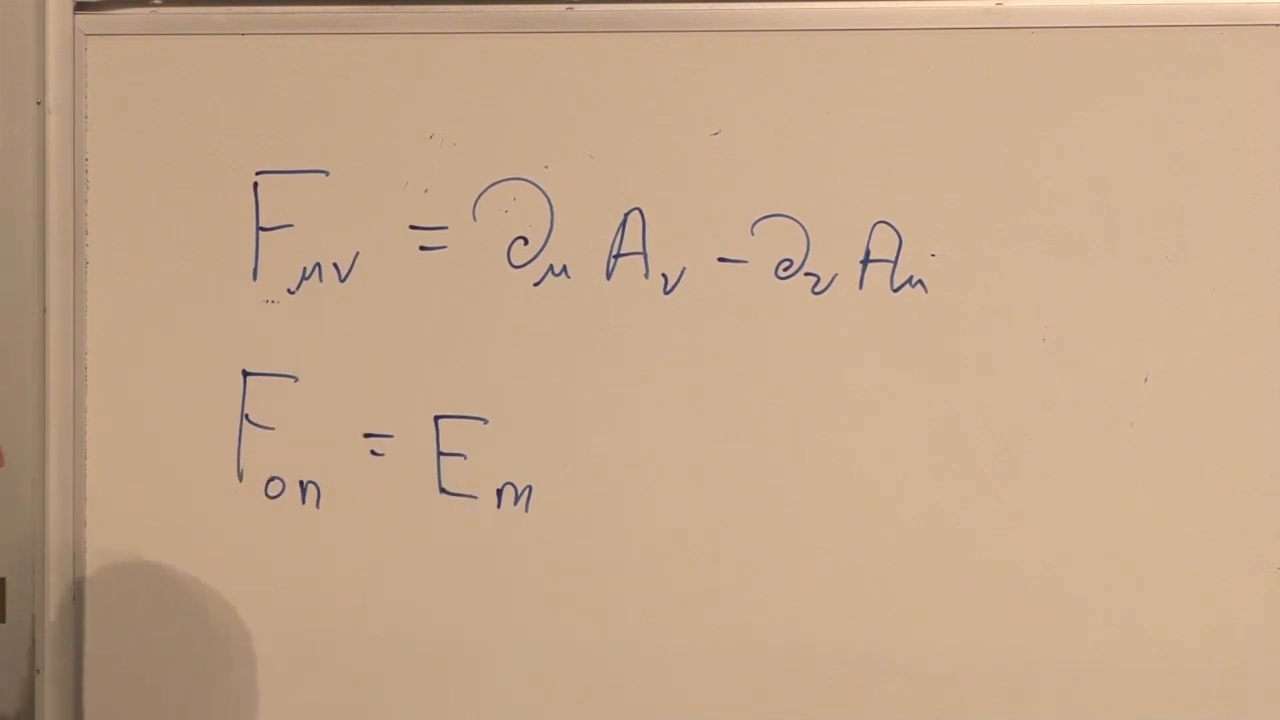
\includegraphics[width=\linewidth]{lecture_08_figure_02.png}\caption{Definition des Feldtensors und seine gemischte Zeit--Raum-Komponente, die mit dem elektrischen Feld identifiziert wird.}\par\smallskip
\textit{Vorlesungsbild: 00:13:15.}\end{figure}

Die Beziehung zum Magnetfeld ist der räumliche Teil derselben Definition. Zum Beispiel gilt
\begin{equation}
B_x
=
\partial_yA_z-\partial_zA_y
=
F_{yz},
\end{equation}
Die beiden anderen Komponenten erhält man durch zyklische Vertauschung.

\begin{figure}[H]\centering
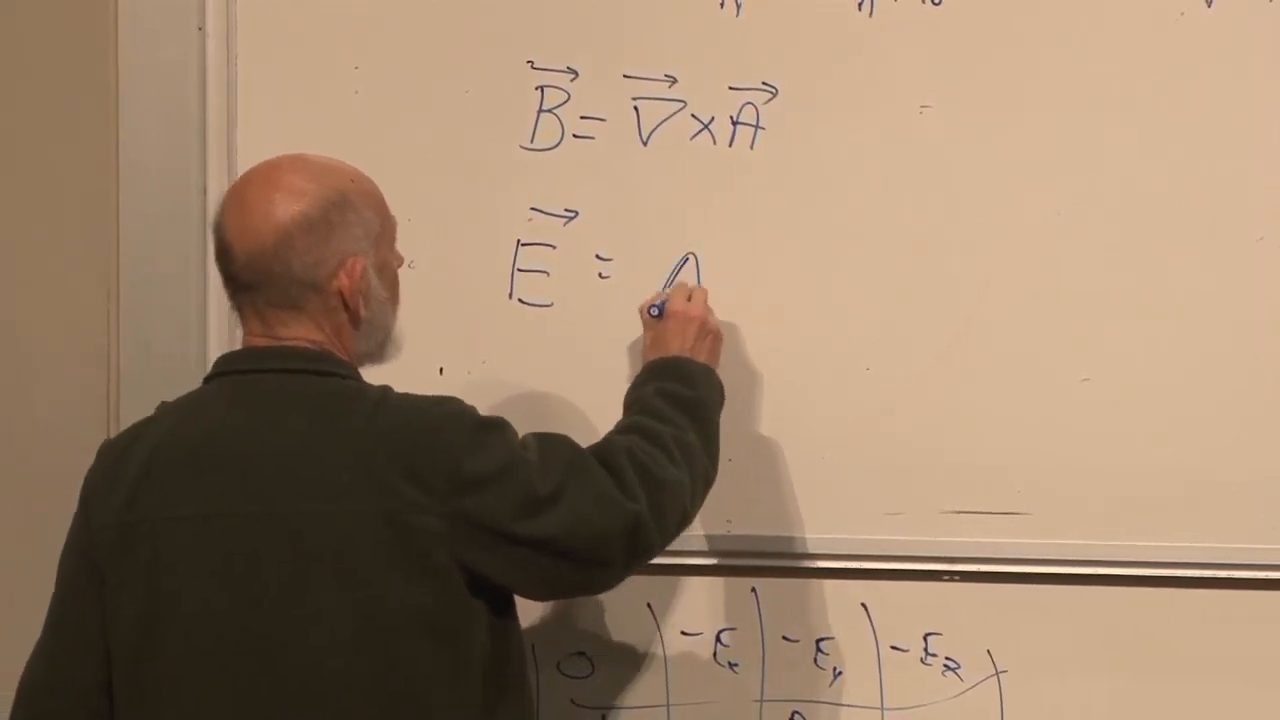
\includegraphics[width=\linewidth]{lecture_08_figure_03.png}\caption{Die Formeln für das elektrische Feld und die Rotation des Vektorpotentials an der Tafel.}\par\smallskip
\textit{Vorlesungsbild: 00:14:00.}\end{figure}

\subsection{Die Komponentenmatrix}

Der erste Tensorindex kennzeichne die Zeilen, der zweite die Spalten, geordnet in der Reihenfolge \(0,x,y,z\). Dann gilt
\begin{equation}
F_{\mu\nu}
=
\begin{pmatrix}
0&E_x&E_y&E_z\\
-E_x&0&B_z&-B_y\\
-E_y&-B_z&0&B_x\\
-E_z&B_y&-B_x&0
\end{pmatrix}.
\label{eq:f-lower-matrix}
\end{equation}
Die gemischte Zeit--Raum-Randkomponente enthält \(\mathbf E\); der räumliche \(3\times3\)-Block enthält \(\mathbf B\). Das untere Dreieck enthält keine neuen Informationen, denn es ist das negative Spiegelbild des oberen Dreiecks.

\begin{figure}[H]\centering
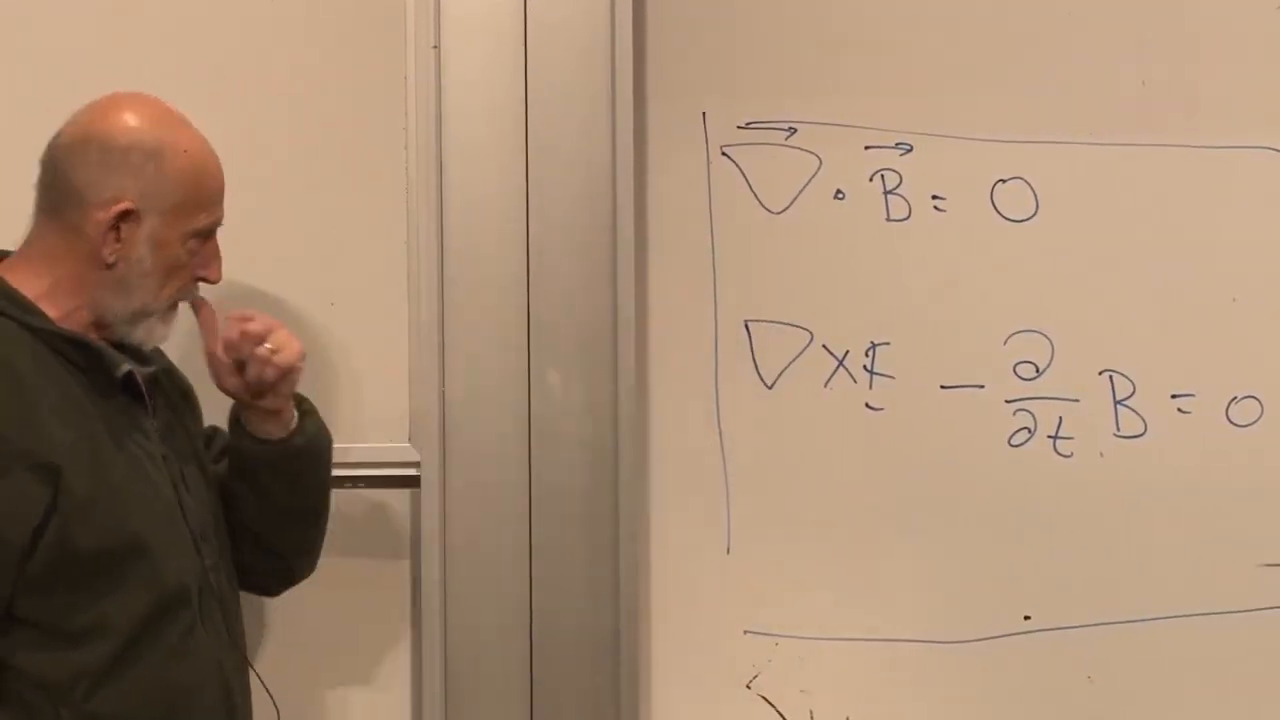
\includegraphics[width=\linewidth]{lecture_08_figure_04.png}\caption{Der vollständig angegebene elektromagnetische Tensor mit unteren Indizes, seinem elektrischen Rand und dem magnetischen räumlichen Block.}\par\smallskip
\textit{Vorlesungsbild: 00:17:15.}\end{figure}

Wenn beide Indizes angehoben werden, ändert sich das Vorzeichen jedes elektrischen Eintrags; die magnetischen Einträge bleiben unverändert:
\begin{equation}
F^{\mu\nu}
=
\begin{pmatrix}
0&-E_x&-E_y&-E_z\\
E_x&0&B_z&-B_y\\
E_y&-B_z&0&B_x\\
E_z&B_y&-B_x&0
\end{pmatrix}.
\label{eq:f-upper-matrix}
\end{equation}
Eine elektrische Komponente enthält einen Zeitindex und erhält daher ein Minuszeichen. Eine magnetische Komponente enthält zwei räumliche Indizes und erhält keines.

\begin{classroomqa}\audiencequestion{Verstehe ich die Matrix richtig: Die magnetischen Komponenten haben keinen Zeitindex?}\lecturerresponse{Ja. Sie liegen im rein räumlichen Block. Die elektrischen Komponenten sind genau die gemischten Zeit--Raum-Einträge in der ersten Zeile und der ersten Spalte. \lecturetimestamp{00:18:55}}\end{classroomqa}

\section{Boost eines rein magnetischen Feldes}

Betrachten wir einen Boost entlang \(x\) mit \(c=1\):
\begin{align}
t'&=\gamma(t-vx),
&
x'&=\gamma(x-vt),
&
y'&=y,
&
z'&=z,
\end{align}
wobei
\begin{equation}
\gamma=\frac{1}{\sqrt{1-v^2}}.
\end{equation}
In Matrixform lautet er
\begin{equation}
x'^\mu
=
\Lambda^\mu{}_\nu x^\nu,
\qquad
\Lambda^\mu{}_\nu
=
\begin{pmatrix}
\gamma&-\gamma v&0&0\\
-\gamma v&\gamma&0&0\\
0&0&1&0\\
0&0&0&1
\end{pmatrix}.
\label{eq:x-boost}
\end{equation}

\begin{classroomqa}\audiencequestion{Fehlt in der Boostmatrix ein Minuszeichen?}\lecturerresponse{Ja. Die außerdiagonalen Zeit--Raum-Einträge tragen die Minuszeichen, die durch \(t'=\gamma(t-vx)\) und \(x'=\gamma(x-vt)\) erforderlich sind. Die Korrektur erfolgt, bevor die Feldtransformation angewendet wird. \lecturetimestamp{00:23:50}}\end{classroomqa}

\begin{figure}[H]\centering
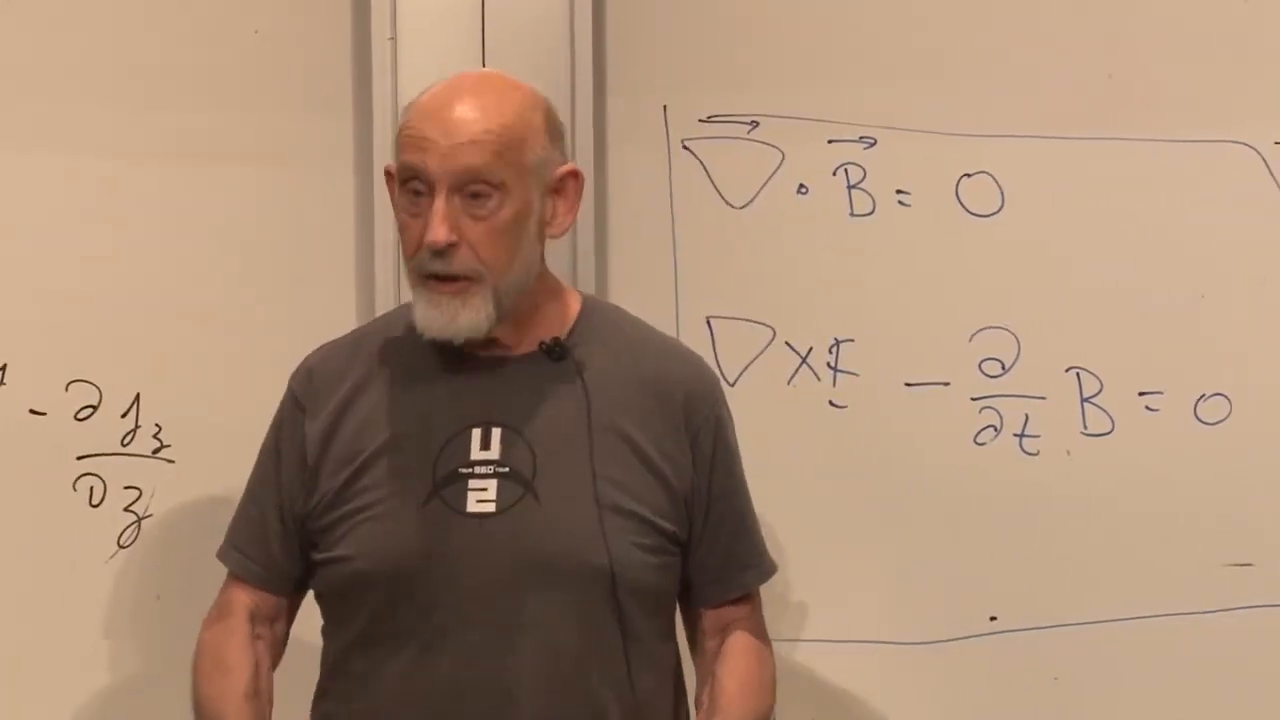
\includegraphics[width=\linewidth]{lecture_08_figure_05.png}\caption{Die korrigierte Lorentz-Boostmatrix für eine Bewegung entlang der \(x\)-Achse.}\par\smallskip
\textit{Vorlesungsbild: 00:24:00.}\end{figure}

Jeder obere Tensorindex transformiert sich wie ein oberer Vektorindex. Daher gilt
\begin{equation}
F'^{\mu\nu}
=
\Lambda^\mu{}_\sigma
\Lambda^\nu{}_\tau
F^{\sigma\tau}.
\label{eq:f-boost-law}
\end{equation}
Die wiederholten Indizes \(\sigma\) und \(\tau\) sind stumme Indizes. Bei einem Tensor mit mehr Indizes tritt für jeden Index eine Transformationsmatrix auf.

\begin{figure}[H]\centering
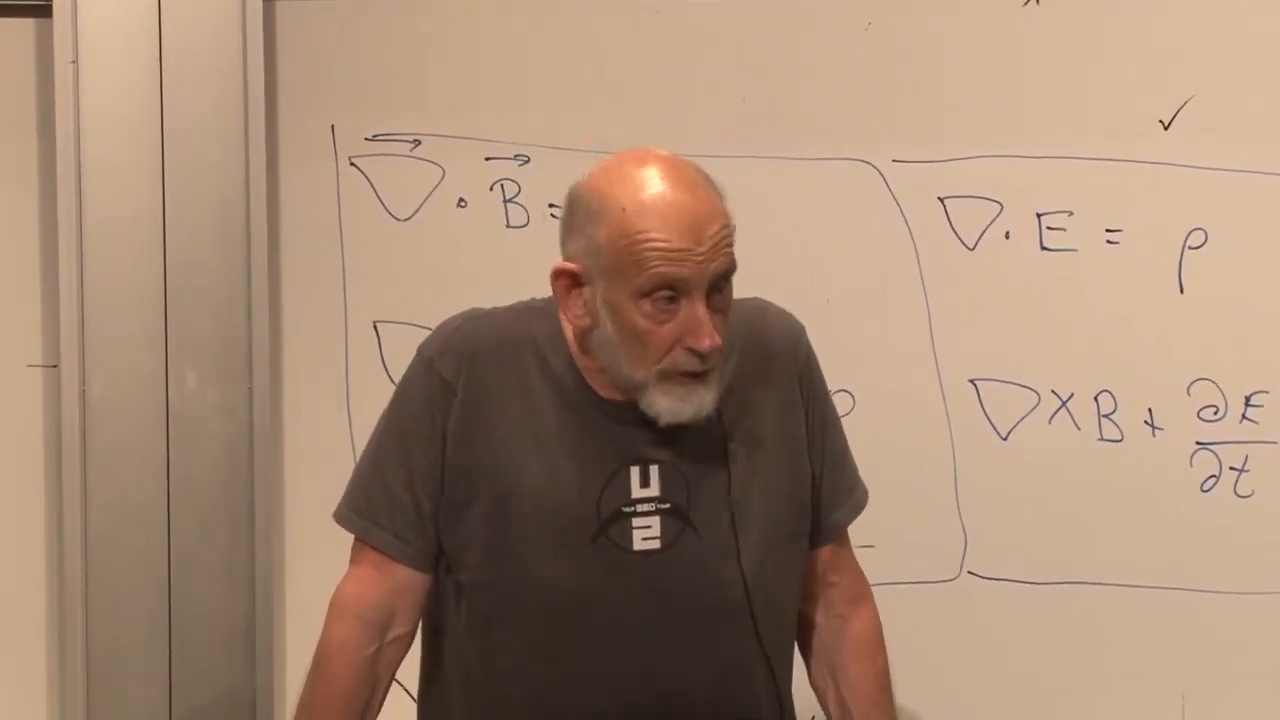
\includegraphics[width=\linewidth]{lecture_08_figure_06.png}\caption{Das Transformationsgesetz für einen Tensor zweiten Ranges unter Lorentz-Transformationen, mit einer Boostmatrix für jeden Index des Feldtensors.}\par\smallskip
\textit{Vorlesungsbild: 00:26:40.}\end{figure}

\subsection{Die Komponente, die elektrisch wird}

Nehmen wir an, das ungestrichene Bezugssystem enthalte nur ein Magnetfeld \(B_y\). Gemäß den Konventionen in Gleichung~\eqref{eq:f-upper-matrix} lautet die relevante unabhängige Komponente
\begin{equation}
F^{xz}=-B_y.
\end{equation}
Gesucht ist die gemischte gestrichene Komponente \(F'^{0z}\), denn sie enthält die gestrichene elektrische Komponente in \(z\)-Richtung. Aus Gleichung
\eqref{eq:f-boost-law} folgt
\begin{align}
F'^{0z}
&=
\Lambda^0{}_\sigma
\Lambda^z{}_\tau F^{\sigma\tau}
\\
&=
\Lambda^0{}_x\Lambda^z{}_zF^{xz}
\\
&=
(-\gamma v)(1)(-B_y)
=
\gamma vB_y.
\end{align}
Da gemäß dieser Konvention \(F'^{0z}=-E'_z\) gilt,
\begin{equation}
E'_z=-\gamma vB_y.
\label{eq:boosted-electric-field}
\end{equation}
Das Vorzeichen hängt von den festgelegten Achsen- und Feldkonventionen ab; der invariante Kern der Rechnung ist
\begin{equation}
\lvert E'_z\rvert
=
\gamma\lvert vB_y\rvert
\ne0.
\end{equation}
Die Doppelsumme reduziert sich darauf, weil das ursprüngliche Feld nur diese eine unabhängige magnetische Komponente besitzt.

\begin{figure}[H]\centering
\includegraphics[width=\linewidth]{lecture_08_figure_07.png}\caption{Die ausgewählte Tensor-Komponente nach dem Boost, mit dem Faktor \(\gamma v\) vor der ursprünglichen magnetischen Komponente.}\par\smallskip
\textit{Vorlesungsbild: 00:32:30.}\end{figure}

Wählen wir das gestrichene Bezugssystem so, dass es sich mit der Ladung bewegt. Dann ruht die Ladung, also gibt es keinen magnetischen Anteil \(q\,\mathbf v'\times\mathbf B'\) ihrer Kraft. Die Kraft verschwindet jedoch nicht: Sie ist \(q\mathbf E'\). Die magnetische Kraft, die der Laborbeobachter beschreibt, und die elektrische Kraft, die der mitbewegte Beobachter beschreibt, sind zwei Beschreibungen desselben Ereignisses.

Damit ist das Rätsel aus Einsteins erstem Absatz gelöst. Die Frage nahm ungefähr die ersten vierzig Minuten dieser Vorlesung ein; der historische Witz dabei ist, dass sie Einstein noch viel länger beschäftigte. Die Rechnung lohnt sich, denn sie macht aus der Aussage, dass sich elektrische und magnetische Felder mischen, eine explizite Tensor-Komponente.

\section{Maxwell-Gleichungen: Identitäten und Dynamik}

Wenden wir uns nun von der Kraft auf eine Ladung den Feldgleichungen zu. In der nächsten Vorlesung werden sie aus einer Wirkung hergeleitet. Hier geht es zunächst darum, sie anzugeben, ihre beiden unterschiedlichen logischen Rollen zu verstehen und den auf Identitäten beruhenden Teil kovariant zu formulieren.

\begin{classroomqa}\audiencequestion{Haben wir diese Gleichungen nicht schon hergeleitet?}\lecturerresponse{Hergeleitet haben wir die Bewegungsgleichung eines geladenen Teilchens in einem vorgegebenen elektromagnetischen Feld. Die Maxwell-Gleichungen sind Bewegungsgleichungen für das Feld selbst, einschließlich seiner Reaktion auf Ladung und Strom. \lecturetimestamp{00:35:10}}\end{classroomqa}

\begin{classroomqa}\audiencequestion{Wie viele Maxwell-Gleichungen gibt es?}\lecturerresponse{Es gibt acht skalare Komponentengleichungen. In Vektorschreibweise fasst man sie als zwei skalare Gleichungen und zwei Vektorgleichungen mit jeweils drei Komponenten zusammen, die man herkömmlich als vier Maxwell-Gleichungen bezeichnet.
\lecturetimestamp{00:35:24}}\end{classroomqa}

Wir verwenden weiterhin Einheiten, in denen \(c=1\) gilt und die üblichen Vakuumkonstanten in die Definitionen von Ladung und Strom aufgenommen wurden. Vier der acht Komponentengleichungen folgen aus der Definition \(F=dA\). Es handelt sich um kinematische Identitäten. Die anderen vier sind dynamisch und könnten sich ändern, wenn sich die Feldwirkung änderte.

\subsection{Drei elementare Vektoroperationen}

Für ein differenzierbares dreidimensionales Vektorfeld \(\mathbf A\) gilt
\begin{align}
(\boldsymbol\nabla\times\mathbf A)_x
&=
\partial_yA_z-\partial_zA_y,
\\
\boldsymbol\nabla\cdot\mathbf A
&=
\partial_xA_x+\partial_yA_y+\partial_zA_z.
\end{align}
Die übrigen Komponenten der Rotation erhält man durch zyklische Vertauschung von \(x\to y\to z\to x\). Für ein skalares Feld \(s\) gilt
\begin{equation}
\boldsymbol\nabla s
=
(\partial_xs,\partial_ys,\partial_zs).
\end{equation}
Die Rotation ist also ein Vektor, die Divergenz ein Skalar und der Gradient ein Vektor.

\begin{classroomqa}\audiencequestion{Muss jemand die Definitionen von Rotation und Divergenz ausführlich wiederholen?}\lecturerresponse{Die Komponentendefinitionen stehen an der Tafel; die übrigen Komponenten müssen nicht alle ausgeschrieben werden. Durch zyklisches Vertauschen der Koordinaten erhält man sie. \lecturetimestamp{00:37:32}}\end{classroomqa}

Aus der Vertauschbarkeit glatter partieller Ableitungen folgen zwei Identitäten:
\begin{align}
\boldsymbol\nabla\cdot
(\boldsymbol\nabla\times\mathbf A)
&=0,
\label{eq:div-curl}
\\
\boldsymbol\nabla\times
(\boldsymbol\nabla s)
&=\mathbf0.
\label{eq:curl-grad}
\end{align}

\begin{classroomqa}\audiencequestion{Sollen wir den vollständigen Komponentenbeweis dafür aufschreiben, dass die Divergenz einer Rotation verschwindet?}\lecturerresponse{Die Klasse verzichtet darauf. Beim Ausmultiplizieren treten Paare wie \(\partial_x\partial_yA_z\) und \(-\partial_y\partial_xA_z\) auf, die sich aufheben, weil sich die Reihenfolge der Ableitungen vertauschen lässt. \lecturetimestamp{00:40:13}}\end{classroomqa}

\begin{figure}[H]\centering
\includegraphics[width=\linewidth]{lecture_08_figure_08.png}\caption{Die Identitäten Divergenz einer Rotation und Rotation eines Gradienten, mit denen sich die eine Hälfte der Maxwell-Gleichungen herleiten lässt.}\par\smallskip
\textit{Vorlesungsbild: 00:41:40.}\end{figure}

\subsection{Keine magnetische Quelle aus dem Vektorpotential}

Bilden wir die Divergenz von Gleichung~\eqref{eq:b-from-a}, so folgt
\begin{equation}
\boldsymbol\nabla\cdot\mathbf B
=
\boldsymbol\nabla\cdot
(\boldsymbol\nabla\times\mathbf A)
=0.
\label{eq:div-b-zero}
\end{equation}
Dabei wurde keine Bewegungsgleichung verwendet. Das Ergebnis folgt allein aus der Potentialbeschreibung und der Vertauschbarkeit glatter Ableitungen.

\begin{figure}[H]\centering
\includegraphics[width=\linewidth]{lecture_08_figure_09.png}\caption{Die Divergenz des Magnetfelds, reduziert auf die Divergenz einer Rotation.}\par\smallskip
\textit{Vorlesungsbild: 00:43:05.}\end{figure}

\begin{classroomqa}\audiencequestion{Was ist die Divergenz des elektrischen Feldes?}\lecturerresponse{In den verwendeten Einheiten ist sie die elektrische Ladungsdichte, \(\boldsymbol\nabla\cdot\mathbf E=\rho\). Eine Punktladung ist das Musterbeispiel für elektrische Feldlinien, die sich von einer Quelle ausbreiten.
\lecturetimestamp{00:43:20}}\end{classroomqa}

Auf elementarer Ebene besagt Gleichung~\eqref{eq:div-b-zero}, dass es keine magnetische Ladungsdichte gibt. Ein glattes, global definiertes Vektorpotential kann keine magnetische Monopolquelle hervorbringen. Diese Aussage muss später eingeschränkt werden: Monopole lassen sich mit Potentialen beschreiben, die auf überlappenden Gebieten definiert sind, oder mit singulären Eichungen. Die Vorlesung verschiebt diese Präzisierung auf später.

\subsection{Die Faraday-Gleichung aus dem elektrischen Potential}

Gleichung~\eqref{eq:e-from-a} lautet in dreidimensionaler Vektorschreibweise
\begin{equation}
\mathbf E
=
\frac{\partial\mathbf A}{\partial t}
-\boldsymbol\nabla A_0.
\label{eq:e-vector-potential}
\end{equation}
Obwohl \(A_0\) zu einem Vierervektor gehört, ist es unter gewöhnlichen räumlichen Drehungen ein Skalar. Bilden wir die Rotation:
\begin{align}
\boldsymbol\nabla\times\mathbf E
&=
\boldsymbol\nabla\times
\frac{\partial\mathbf A}{\partial t}
-
\boldsymbol\nabla\times
(\boldsymbol\nabla A_0)
\\
&=
\frac{\partial}{\partial t}
(\boldsymbol\nabla\times\mathbf A)
\\
&=
\frac{\partial\mathbf B}{\partial t}.
\end{align}
Die räumliche Rotation vertauscht mit der Zeitableitung, während die Rotation des Gradienten verschwindet.

\begin{figure}[H]\centering
\includegraphics[width=\linewidth]{lecture_08_figure_10.png}\caption{Die Rotation des Magnetfelds, die Formel des elektrischen Feldes mit dem Potential und der Beginn der Rotationsrechnung in einem fertigen Tafelbild.}\par\smallskip
\textit{Vorlesungsbild: 00:47:45.}\end{figure}

Die vier homogenen Komponentengleichungen lauten somit
\begin{align}
\boldsymbol\nabla\cdot\mathbf B&=0,
\label{eq:homogeneous-div}
\\
\boldsymbol\nabla\times\mathbf E
-\frac{\partial\mathbf B}{\partial t}
&=\mathbf0.
\label{eq:homogeneous-curl}
\end{align}
Die erste ist eine skalare Gleichung, die zweite eine Vektorgleichung mit drei Komponenten.

\begin{figure}[H]\centering
\includegraphics[width=\linewidth]{lecture_08_figure_11.png}\caption{Das quellenfreie Maxwell-Paar, direkt aus den Potentialdefinitionen erhalten.}\par\smallskip
\textit{Vorlesungsbild: 00:48:45.}\end{figure}

\subsection{Der dynamische Teil}

Die übrigen Gleichungen lauten
\begin{align}
\boldsymbol\nabla\cdot\mathbf E&=\rho,
\label{eq:gauss-electric}
\\
\boldsymbol\nabla\times\mathbf B
+\frac{\partial\mathbf E}{\partial t}
&=-\mathbf J.
\label{eq:ampere-maxwell}
\end{align}
Sie folgen nicht aus \(F=dA\). Sie beschreiben, wie Quellen das Feld erzeugen und verändern; in der nächsten Vorlesung werden sie aus der elektromagnetischen Wirkung hergeleitet. Das Minuszeichen vor dem Strom ergibt sich aus den bereits gewählten Konventionen: \(F_{0i}=E_i\), \(F_{ij}=\epsilon_{ijk}B_k\) und \(\partial_\mu F^{\mu\nu}=J^\nu\). An der Tafel steht zunächst \(\mathbf J\) ohne dieses Minuszeichen auf der rechten Seite; die daraus folgende Unvereinbarkeit mit der Ladungserhaltung wird in der nächsten Vorlesung bemerkt und korrigiert.

\begin{classroomqa}\audiencequestion{Welche Art von Größe steht auf der rechten Seite der Rotationsgleichung?}\lecturerresponse{Die linke Seite ist ein dreidimensionaler Vektor, also ist auch die rechte Seite ein dreidimensionaler Vektor, die elektrische Stromdichte \(\mathbf J\). Auf der rechten Seite der Gauß-Gleichung steht die dreidimensionale skalare Ladungsdichte \(\rho\).
\lecturetimestamp{00:50:36}}\end{classroomqa}

\begin{figure}[H]\centering
\includegraphics[width=\linewidth]{lecture_08_figure_12.png}\caption{Die vier Maxwell-Gleichungen, gruppiert in das auf Identitäten beruhende Paar und das dynamische Paar mit Quellen.}\par\smallskip
\textit{Vorlesungsbild: 00:50:40.}\end{figure}

\section{Ladung und Strom als Raumzeitfluss}

Den Größen \(\rho\) und \(\mathbf J\) müssen nun geometrische Bedeutungen zugewiesen werden. Die Ladungsdichte ist Ladung pro Volumeneinheit; die Stromdichte ist die Ladung, die pro Zeiteinheit eine orientierte Fläche durchquert. Die Vorlesung entwickelt beide Größen aus Weltlinien, damit ihre spätere Zusammenfassung zu einem Vierervektor nicht zufällig erscheint.

\subsection{Eine Randbemerkung aus dem benachbarten Hörsaal}

Bevor wir diese Weltlinien zeichnen, geben Gleichungen, die an der Tafel im Nachbarraum zu sehen sind, Anlass zu einer kurzen didaktischen Randbemerkung. In einem bevorstehenden Kurs sollte Mathematikdozenten Quantenmechanik vermittelt werden, damit sie die nötigen Vorkenntnisse für die Quantenfeldtheorie und deren Verbindungen zur modernen Mathematik erwerben konnten. Die Herausforderung wirkt in beide Richtungen: Der Physiker muss unausgesprochene physikalische Denkweisen explizit machen, während der Mathematiker verstehen muss, was die formalen Strukturen beschreiben sollen.

\begin{classroomqa}\audiencequestion{Wer dürfte diesen Lehrauftrag als frustrierend empfinden?}\lecturerresponse{Möglicherweise beide Seiten: Physiker, die vor einem unvertrauten Publikum lehren, und Mathematiker, die sich mit den physikalischen Denkweisen hinter dem Formalismus auseinandersetzen. Dennoch dürfte der Lehrauftrag Spaß machen. Dann kehrt die Klasse zu Ladung und Strom zurück. \lecturetimestamp{00:53:20}}\end{classroomqa}

\subsection{Ladungsdichte}

Zeichnen wir die Zeit senkrecht und fassen die übrigen gezeichneten Richtungen als dreidimensionalen Raum auf. Geladene Teilchen beschreiben Weltlinien. Wählen wir zu einem festen Zeitpunkt einen kleinen räumlichen Würfel mit Volumen \(\Delta V\), der die Gesamtheit dieser Weltlinien durchschneidet, und addieren wir die Ladungen der Teilchen darin. Die Ladungsdichte ist dann
\begin{equation}
\rho(t,\mathbf x)
=
\lim_{\Delta V\to0}
\frac{\Delta Q}{\Delta V}.
\label{eq:charge-density}
\end{equation}
Das zweidimensionale Quadrat an der Tafel stellt einen dreidimensionalen Würfel dar; die fehlende räumliche Richtung wird nur deshalb nicht gezeichnet, weil sich vier Dimensionen nicht auf einer flachen Tafel darstellen lassen.

\begin{figure}[H]\centering
\includegraphics[width=\linewidth]{lecture_08_figure_13.png}\caption{Weltlinien geladener Teilchen, die eine kleine räumliche Zelle durchqueren, mit \(\rho=\Delta Q/\Delta V\).}\par\smallskip
\textit{Vorlesungsbild: 00:57:20.}\end{figure}

\subsection{Stromdichte}

Drehen wir die Raumzeitzelle auf die Seite. Um \(J_x\) zu definieren, wählen wir ein kleines Fenster mit der Fläche \(\Delta A_x\) in der \(yz\)-Ebene, senkrecht zur \(x\)-Achse. Wir zählen die Nettoladung, die während \(\Delta t\) von der negativen \(x\)-Seite zur positiven \(x\)-Seite übertritt:
\begin{equation}
J_x
=
\lim_{\Delta A_x,\Delta t\to0}
\frac{\Delta Q_x}{\Delta A_x\,\Delta t}.
\label{eq:jx-window}
\end{equation}
Die Orientierung legt das Vorzeichen fest. Fenster senkrecht zu \(y\) und \(z\) definieren auf dieselbe Weise \(J_y\) und \(J_z\).

Die Zeichnung an der Tafel gerät ins Ringen mit der Darstellung: Ein Fenster in der \(yz\)-Ebene sieht eher wie ein Fenster in der Decke als in der Wand aus. Es gibt schlicht mehr relevante Achsen, als sich gleichzeitig darstellen lassen. Die invariante Definition ist eindeutig, auch wenn die Skizze es nicht ist.

\begin{classroomqa}\audiencequestion{Liegt das Fenster in der Zeichnung an der Decke?}\lecturerresponse{In der Analogie mit dem Raum: ja. Entscheidend ist, dass seine Ebene senkrecht zur Richtung \(x\) steht. Eine Fläche \(yz\) misst den Strom in \(x\)-Richtung, der sie durchquert. \lecturetimestamp{00:59:38}}\end{classroomqa}

\begin{figure}[H]\centering
\includegraphics[width=\linewidth]{lecture_08_figure_14.png}\caption{Ladungsstrom durch ein transversales Fenster, mit \(J_x=\Delta Q/(\Delta A\,\Delta t)\).}\par\smallskip
\textit{Vorlesungsbild: 01:01:40.}\end{figure}

\begin{figure}[H]\centering
\includegraphics[width=\linewidth]{lecture_08_figure_15.png}\caption{Die drei Stromkomponenten, definiert über Ladung, die Fenster senkrecht zu den drei räumlichen Achsen durchquert.}\par\smallskip
\textit{Vorlesungsbild: 01:02:40.}\end{figure}

Die vier Größen sind analog definiert. Ein räumliches Volumen zu einem festen Zeitpunkt ist eine Hyperfläche senkrecht zur Zeitachse, sodass \(\rho\) den Ladungsfluss durch ein zeitnormales Fenster angibt. Die Größen \(J_i\) beschreiben Flüsse durch räumlich normale Fenster.

\begin{classroomqa}\audiencequestion{Sind die vier Zahlen ein Fluss in Zeitrichtung und drei Flüsse in den räumlichen Richtungen?}\lecturerresponse{Genau das ist die hilfreiche Vorstellung. Ein räumliches Volumen ist ein Fenster senkrecht zur Zeitachse; die drei transversalen Flächen sind Fenster senkrecht zu \(x\), \(y\) und \(z\). Diese vier Flüsse gehören zusammen. \lecturetimestamp{01:04:14}}\end{classroomqa}

Das legt den kontravarianten Viererstrom nahe:
\begin{equation}
J^\mu
=
(\rho,J_x,J_y,J_z).
\label{eq:four-current}
\end{equation}

\begin{classroomqa}\audiencequestion{Wo kommt die Metrik ins Spiel, und ist dieser Strom kovariant oder kontravariant?}\lecturerresponse{Wie hier definiert, bilden \(\rho\) und die drei Größen \(J_i\) die Komponenten von \(J^\mu\), einem Vierervektor mit oberen Indizes, also einem kontravarianten Vierervektor. Die Metrik senkt den Index, wenn \(J_\mu\) benötigt wird. Die kovariante Formulierung der Maxwell-Gleichungen wird zeigen, warum die Wahl oberer Indizes naheliegt.
\lecturetimestamp{01:04:48}}\end{classroomqa}

\section{Zwischenspiel in der Pause: Signale nahe einem Schwarzen Loch}

In der angesetzten Pause wenden sich die Fragen einer früheren Diskussion über Schwarze Löcher zu. Diese Abschweifung von der Elektrodynamik ist ein ausführlicher Austausch im Hörsaal und veranschaulicht dieselbe Sorgfalt, mit der Beschreibungen verschiedener Beobachter auseinandergehalten werden.

\begin{classroomqa}\audiencequestion{Wenn ein weit entfernter Beobachter sieht, wie ein hineinfallendes Objekt nahe dem Horizont langsamer wird, müsste das Schwarze Loch dann nicht von allem bedeckt erscheinen, was jemals hineingefallen ist?}\lecturerresponse{In der Schwarzschild-Koordinatenzeit scheint klassischer freier Fall den Horizont asymptotisch zu erreichen. Man kann sich aufeinanderfolgende Materie als immer stärker komprimierte Schichten nahe dem Horizont vorstellen. Beobachtbar verzögert sich das ausgesandte Signal jedoch zunehmend, wird rotverschoben und schwächer. Licht, das lokal mit einer gewöhnlichen Frequenz ausgesandt wird, kommt zunächst als sichtbares Licht, dann als Infrarot-, Mikrowellen- und schließlich als Radiostrahlung an; jedes Photon trägt dabei weniger Energie. Kein realistischer weit entfernter Detektor kann ein helles, eingefrorenes Objekt für immer sehen; es verblasst in der Schwärze.
\lecturetimestamp{01:06:11}}\end{classroomqa}

Die Uhr des hineinfallenden Beobachters und die lokal ausgesandte Taschenlampenstrahlung bleiben für diesen Beobachter gewöhnlich. Die Beschreibung aus der Ferne weicht ab, weil sowohl die Frequenz als auch die Ankunftsrate rotverschoben werden. Bei endlicher Energie und endlicher Bandbreite gibt es effektiv einen letzten noch auflösbaren Teil der Nachricht.

\begin{classroomqa}\audiencequestion{Nähert sich das Objekt asymptotisch dem Ereignishorizont?}\lecturerresponse{Das ist die Beschreibung aus der Ferne in Schwarzschild-Koordinaten. Quantentheoretisch muss man das verblassende Signal außerdem von der Hawking-Strahlung des Schwarzen Lochs unterscheiden. Zu hinreichend späten Zeiten geht das schwache rotverschobene Signal in der Hintergrundstrahlung des Schwarzen Lochs selbst beobachtbar verloren. \lecturetimestamp{01:09:24}}\end{classroomqa}

\begin{classroomqa}\audiencequestion{Was, wenn die Wellenlänge der rotverschobenen Strahlung größer wird als die Skala des beobachtbaren Universums?}\lecturerresponse{Praktisch geht das Signal lange vor Erreichen dieser Grenze verloren. Die Vorlesung gibt als grobe Größenordnung für das Hawking-Bild ungefähr ein typisches Quant pro Lichtdurchquerungszeit an:
\[
t_{\rm cross}\sim\frac{R_s}{c}.
\]
Für ein großes Schwarzes Loch ist diese Strahlung außerordentlich schwach, und ein hinreichend stark rotverschobenes Signal des hineinfallenden Objekts wird lange vor jeder kosmologischen Grenze für die Wellenlänge undetektierbar. \lecturetimestamp{01:09:50}}\end{classroomqa}

\begin{classroomqa}\audiencequestion{Bleibt die Rate von ungefähr einem Quant pro Durchquerungszeit während der gesamten Lebensdauer des Schwarzen Lochs gleich?}\lecturerresponse{Nein. Ein verdampfendes Schwarzschild-Schwarzes-Loch schrumpft, sodass seine Durchquerungszeit kürzer und seine Hawking-Temperatur höher wird. Die Emission beschleunigt sich daher. Die Dimensionsabschätzung anhand des momentanen Radius bleibt nützlich, aber der Radius ist nicht konstant. Entsprechend wird die typische Hawking-Wellenlänge im Verlauf der Verdampfung kürzer. \lecturetimestamp{01:11:42}}\end{classroomqa}

Nach der Pause kehren wir, ohne Jackett, zu \(\rho\) und \(\mathbf J\) zurück.

\section{Lokale Ladungserhaltung}

Es liegt nahe, Ladungserhaltung lediglich so anzugeben:
\begin{equation}
\frac{dQ_{\rm universe}}{dt}=0.
\end{equation}
Diese Aussage ist zu schwach. Ladung könnte aus einem Labor verschwinden und sofort bei Alpha Centauri oder noch weiter entfernt im Coma-Haufen wieder auftauchen, ohne dass sich die Gesamtladung änderte. Ein solches Gesetz hätte kaum experimentelle Aussagekraft.

Die stärkere Aussage ist lokal: Die Ladung in einem Gebiet kann sich nur dadurch ändern, dass Ladung die Grenze dieses Gebiets überquert. Legen wir einen kleinen Kasten um einen Punkt. Nimmt seine Ladung zu, muss durch seine sechs Seitenflächen netto einwärts gerichteter Strom fließen; nimmt sie ab, muss netto Strom nach außen fließen.

\subsection{Fluss durch gegenüberliegende Flächen}

Betrachten wir die beiden Flächen senkrecht zu \(x\). Der Beitrag nach innen auf der einen Fläche wird bei einem bestimmten Wert von \(x\) ausgewertet; der Beitrag auf der gegenüberliegenden Fläche wird bei einem geringfügig entfernten Wert ausgewertet. Ihre Differenz, geteilt durch die Breite des Kastens, geht über in
\begin{equation}
-\partial_xJ_x.
\end{equation}
Das Minuszeichen tritt auf, weil \(J_x\) als Fluss in Richtung zunehmender \(x\) definiert ist, während ein nach außen gerichteter Fluss die Ladung im Kasten verringert. Die Paare der \(y\)- und \(z\)-Flächen tragen entsprechend \(-\partial_yJ_y\) und \(-\partial_zJ_z\) bei. Daher gilt
\begin{equation}
\frac{\partial\rho}{\partial t}
=
-\partial_xJ_x-\partial_yJ_y-\partial_zJ_z
=
-\boldsymbol\nabla\cdot\mathbf J.
\end{equation}
Äquivalent dazu:
\begin{equation}
\boxed{
\frac{\partial\rho}{\partial t}
+\boldsymbol\nabla\cdot\mathbf J=0
}.
\label{eq:continuity}
\end{equation}

\begin{figure}[H]\centering
\includegraphics[width=\linewidth]{lecture_08_figure_16.png}\caption{Das lokale Bilanzgesetz \(\dot\rho=-\boldsymbol\nabla\cdot\mathbf J\) zusammen mit dem kleinen Kasten, dessen Randströme es hervorbringen.}\par\smallskip
\textit{Vorlesungsbild: 01:20:45.}\end{figure}

Dies wird üblicherweise Kontinuitätsgleichung genannt. In der Vorlesung wird die Bezeichnung \emph{lokale Erhaltung} bevorzugt: „Kontinuität“ kann eine mathematische Glattheitsannahme nahelegen, während der physikalische Inhalt darin besteht, dass Ladung nicht hier verschwinden und dort wieder auftauchen kann, ohne dass dazwischen ein Strom fließt.

\subsection{Warum Maxwell den Verschiebungsstrom benötigte}

Gleichung~\eqref{eq:continuity} ist keine unabhängige Ergänzung der Maxwell-Gleichungen. Wir bilden die Zeitableitung des Gaußschen Gesetzes und die Divergenz des Ampère--Maxwell-Gesetzes:
\begin{align}
\frac{\partial\rho}{\partial t}
&=
\boldsymbol\nabla\cdot
\frac{\partial\mathbf E}{\partial t},
\\
-\boldsymbol\nabla\cdot\mathbf J
&=
\boldsymbol\nabla\cdot
(\boldsymbol\nabla\times\mathbf B)
+
\boldsymbol\nabla\cdot
\frac{\partial\mathbf E}{\partial t}
\\
&=
\boldsymbol\nabla\cdot
\frac{\partial\mathbf E}{\partial t}.
\end{align}
Die beiden linken Seiten sind daher gleich, woraus
\(\partial_t\rho=-\boldsymbol\nabla\cdot\mathbf J\) folgt – genau
Gleichung~\eqref{eq:continuity}. Entscheidend ist hier die Struktur: Die Zeitableitung von \(\mathbf E\), der Verschiebungsstromterm, ist wesentlich, damit die Divergenzrelation mit der Ladungserhaltung vereinbar ist.

\begin{classroomqa}
\audiencequestion{Wir haben doch nicht gezeigt, woher die beiden quellenbehafteten Maxwell-Gleichungen kommen, oder?}
\lecturerresponse{Nein. Sie sind das dynamische Ziel und werden nächstes Mal aus der Wirkung hergeleitet. Das magnetostatische Wirbelgesetz war schon vor Maxwell bekannt; Maxwells entscheidende zeitabhängige Ergänzung war der Verschiebungsstrom. Durch ihn ist die Feldgleichung mit der lokalen Ladungserhaltung vereinbar. \lecturetimestamp{01:23:15}}
\end{classroomqa}

Die ausführliche Divergenzrechnung wird in der Vorlesung als Übung überlassen, aber ihre Schlussfolgerung ist zwingend: Die Maxwell-Gleichungen erfordern Ladungserhaltung.

\section{Der Viererstrom und seine Divergenz}

Schreiben wir Gleichung~\eqref{eq:continuity} komponentenweise:
\begin{equation}
\frac{\partial\rho}{\partial t}
+
\frac{\partial J_x}{\partial x}
+
\frac{\partial J_y}{\partial y}
+
\frac{\partial J_z}{\partial z}
=0.
\label{eq:continuity-components}
\end{equation}

\begin{figure}[H]
\centering
\includegraphics[width=\linewidth]{lecture_08_figure_17.png}
\caption{Die lokale Ladungserhaltung, aufgeschlüsselt in eine Zeitableitung und drei räumliche Ableitungen.}
\par\smallskip
\textit{Vorlesungszeit: 01:25:40.}
\end{figure}

Mit \(J^\mu\), definiert durch Gleichung~\eqref{eq:four-current}, lassen sich die vier Terme zu einer Kontraktion zusammenfassen:
\begin{equation}
\boxed{\partial_\mu J^\mu=0}.
\label{eq:four-current-conservation}
\end{equation}
Der untere Index von \(\partial_\mu\) wird mit dem oberen Index von \(J^\mu\) kontrahiert; das Ergebnis ist daher ein Lorentz-Skalar. Die geometrische Konstruktion des Fensters deutete dieses Transformationsgesetz bereits an: \(\rho\) und die drei Stromkomponenten sind vier Orientierungen desselben Ladungsflusses.

\begin{figure}[H]
\centering
\includegraphics[width=\linewidth]{lecture_08_figure_18.png}
\caption{Die Komponenten \((\rho,J_x,J_y,J_z)\) werden zu \(J^\mu\) zusammengesetzt und mit dem Vierergradienten kontrahiert.}
\par\smallskip
\textit{Vorlesungszeit: 01:27:10.}
\end{figure}

\begin{classroomqa}
\audiencequestion{Wann wurde aus der Zeitableitung von \(\rho\) eine partielle Ableitung?}
\lecturerresponse{Sie war von Anfang an eine partielle Ableitung. Wir halten das räumliche Kästchen fest und fragen, wie sich seine Ladungsdichte mit der Zeit verändert. Wir verfolgen keine bewegte Bahn. Daher bedeutet \(\dot\rho\) hier \(\partial\rho/\partial t\) bei festgehaltenem \(x,y,z\).
\lecturetimestamp{01:28:20}}
\end{classroomqa}

\section{Die homogenen Gleichungen in kovarianter Form}

Wir verfügen nun über die benötigten Größen:
\begin{itemize}
\item \(\mathbf E\) und \(\mathbf B\) sind die sechs unabhängigen Komponenten des antisymmetrischen Tensors \(F_{\mu\nu}\);
\item \(\rho\) und \(\mathbf J\) sind die vier Komponenten von \(J^\mu\);
\item die lokale Erhaltung ist die skalare Gleichung
\(\partial_\mu J^\mu=0\).
\end{itemize}
Als verbleibende Aufgabe für diese Vorlesung müssen wir das Paar homogener Maxwell-Gleichungen, Gleichungen~\eqref{eq:homogeneous-div} und
\eqref{eq:homogeneous-curl}, in einer einzigen Tensor-Gleichung zusammenfassen.

\subsection{Die zyklische Ableitung}

Die gesuchte Gleichung lautet
\begin{equation}
\boxed{
\partial_\sigma F_{\nu\tau}
+
\partial_\nu F_{\tau\sigma}
+
\partial_\tau F_{\sigma\nu}
=0
}.
\label{eq:bianchi}
\end{equation}
In den drei Termen werden der Ableitungsindex und die beiden Indizes des Feldtensors zyklisch vertauscht. Oft schreibt man dies abgekürzt als
\begin{equation}
\partial_{[\sigma}F_{\nu\tau]}=0,
\end{equation}
wobei eckige Klammern die Antisymmetrisierung bezeichnen.

\begin{figure}[H]
\centering
\includegraphics[width=\linewidth]{lecture_08_figure_19.png}
\caption{Die zyklische Gleichung mit drei Indizes, die die homogenen Maxwell-Gleichungen zusammenfasst.}
\par\smallskip
\textit{Vorlesungszeit: 01:33:20.}
\end{figure}

\subsection{Alle drei Indizes räumlich}

Setzen wir
\begin{equation}
(\sigma,\nu,\tau)=(x,y,z).
\end{equation}
Dann gilt
\begin{align}
0
&=
\partial_xF_{yz}
+
\partial_yF_{zx}
+
\partial_zF_{xy}
\\
&=
\partial_xB_x+\partial_yB_y+\partial_zB_z
\\
&=
\boldsymbol\nabla\cdot\mathbf B.
\end{align}
Die Komponente von Gleichung~\eqref{eq:bianchi}, bei der alle Indizes räumlich sind, besagt somit genau, dass die magnetische Divergenz verschwindet.

\begin{figure}[H]
\centering
\includegraphics[width=\linewidth]{lecture_08_figure_20.png}
\caption{Die Komponente der zyklischen Identität mit ausschließlich räumlichen Indizes reduziert sich auf \(\partial_xB_x+\partial_yB_y+\partial_zB_z=0\).}
\par\smallskip
\textit{Vorlesungszeit: 01:35:30.}
\end{figure}

\subsection{Ein Zeitindex}

Wählen wir beispielsweise
\begin{equation}
(\sigma,\nu,\tau)=(y,x,0).
\end{equation}
Dann verbindet Gleichung~\eqref{eq:bianchi} zwei räumliche Ableitungen elektrischer Komponenten mit einer Zeitableitung einer magnetischen Komponente:
\begin{equation}
\partial_yF_{x0}
+
\partial_xF_{0y}
+
\partial_0F_{yx}
=0.
\end{equation}
Mit der Matrix aus Gleichung~\eqref{eq:f-lower-matrix} ist dies eine Komponente von
\begin{equation}
\boldsymbol\nabla\times\mathbf E
-\frac{\partial\mathbf B}{\partial t}
=\mathbf0,
\end{equation}
wobei die relativen Vorzeichen durch die Antisymmetrie festgelegt sind. Die Wahl der anderen Paare räumlicher Indizes liefert die beiden übrigen Komponenten der Rotation.

\begin{figure}[H]
\centering
\includegraphics[width=\linewidth]{lecture_08_figure_21.png}
\caption{Eine Prüfung mit einem Zeitindex und zwei Raumindizes ergibt eine Komponente der Faraday-Gleichung.}
\par\smallskip
\textit{Vorlesungszeit: 01:38:20.}
\end{figure}

Es gibt auch einen direkten Beweis. Setzen wir Gleichung~\eqref{eq:field-tensor-definition} in Gleichung~\eqref{eq:bianchi} ein. Dabei entstehen sechs Terme mit zweiten Ableitungen, die sich paarweise aufheben, weil partielle Ableitungen vertauschbar sind. Dies ist die vierdimensionale Version der Identitäten für die Divergenz einer Rotation und die Rotation eines Gradienten.

\begin{classroomqa}
\audiencequestion{Kommt im Namen Bianchi ein \(h\) vor?}
\lecturerresponse{Ja. Die zyklische Gleichung ist die elektromagnetische Bianchi-Identität, ein Spezialfall einer geometrischen Identität, die auch in der allgemeinen Relativitätstheorie auftritt. Ihre tiefere geometrische Deutung wird später behandelt.
\lecturetimestamp{01:40:28}}
\end{classroomqa}

\subsection{Warum vierundsechzig hingeschriebene Komponenten nur vier Gleichungen enthalten}

Drei Indizes mit jeweils vier möglichen Werten scheinen \(4^3=64\) Gleichungen zu ergeben. Die Antisymmetrie beseitigt die Redundanz:
\begin{itemize}
\item Wenn zwei Indizes übereinstimmen, verschwindet der zyklische Ausdruck identisch;
\item Sind alle drei Indizes verschieden, ergeben Permutationen bis auf ein Vorzeichen dieselbe Gleichung;
\item In vier Dimensionen gibt es nur \(\binom{4}{3}=4\) ungeordnete Tripel verschiedener Indizes.
\end{itemize}
Es gibt \(24\) geordnete Tripel mit lauter verschiedenen Indizes; sie gruppieren sich in vier Mengen aus jeweils sechs Permutationen. Die übrigen \(40\) geordneten Tripel verschwinden. Die vier unabhängigen Gleichungen bestehen aus einer Gleichung für die magnetische Divergenz und den drei Komponenten der Faraday-Gleichung.

\begin{classroomqa}
\audiencequestion{Der Feldtensor hat sechs unabhängige Einträge, aber der Ausdruck mit drei Indizes scheint vierundsechzig Gleichungen zu enthalten. Warum bleiben nur vier übrig?}
\lecturerresponse{Bei wiederholten Indizes ergibt sich null; Permutationen dreier verschiedener Indizes wiederholen dieselbe Relation bis auf ein Vorzeichen. Die scheinbar vierundsechzig Komponenten reduzieren sich daher auf vier unabhängige Gleichungen.
\lecturetimestamp{01:41:58}}
\end{classroomqa}

Gleichung~\eqref{eq:bianchi} ist offensichtlich tensorial und damit Lorentz-kovariant. In der glatten Beschreibung mit einem einzigen Potential besagt sie außerdem, dass es weder eine magnetische Ladungsdichte noch einen magnetischen Strom gibt. Das dynamische, quellenbehaftete Gleichungspaar bleibt genau an dem Punkt, den die Vorlesung erreicht hat: Seine kovariante Gleichung und ihre Herleitung aus der Wirkung folgen in der nächsten Sitzung.

\section{Dualität und die Frage nach dem Monopol}

Die abschließenden Fragen greifen die scheinbare Asymmetrie zwischen elektrischen und magnetischen Quellen wieder auf. Im leeren Raum besitzen die Maxwell-Gleichungen eine elektrische--magnetische Dualitätsdrehung:
\begin{equation}
\mathbf E\longrightarrow\mathbf B,
\qquad
\mathbf B\longrightarrow-\mathbf E.
\label{eq:duality-quarter-turn}
\end{equation}
Dies ist eine Drehung um neunzig Grad in einer abstrakten Ebene mit den Achsen \(\mathbf E\) und \(\mathbf B\), keine Spiegelung, die lediglich ihre Bezeichnungen vertauscht. Sind sowohl elektrische als auch magnetische Quellen vorhanden, müssen sich die elektrischen und magnetischen Viererströme gleichzeitig mitdrehen.

\begin{figure}[H]
\centering
\includegraphics[width=\linewidth]{lecture_08_figure_22.png}
\caption{Die abschließende elektrische--magnetische Dualitätsdarstellung: eine Vierteldrehung in der \(E\)-\(B\)-Ebene statt einer bloßen Vertauschung.}
\par\smallskip
\textit{Vorlesungszeit: 01:45:00.}
\end{figure}

\begin{classroomqa}
\audiencequestion{Wenn die quellenfreien Gleichungen unter der Vertauschung von elektrisch und magnetisch dual sind, warum sind dann die elektrischen Komponenten Zeit--Raum-Einträge, während die magnetischen Komponenten Raum--Raum-Einträge sind?}
\lecturerresponse{Die Unterscheidung hängt innerhalb von \(F_{\mu\nu}\) vom Bezugssystem ab, und die quellenfreien Gleichungen lassen eine Dualitätsdrehung zu. Die richtige Operation ist \(\mathbf E\to\mathbf B\) und \(\mathbf B\to-\mathbf E\); werden magnetische Ladungen berücksichtigt, müssen sich die Quellenströme entsprechend mitdrehen. Eine bloße Vertauschung lässt das erforderliche Vorzeichen außer Acht. \lecturetimestamp{01:43:25}}
\end{classroomqa}

\begin{classroomqa}
\audiencequestion{Macht die klare Tensorbeschreibung einen magnetischen Monopol bedeutungslos?}
\lecturerresponse{Nein. Sie bedeutet, dass sich ein Monopol nicht mit einem einzigen glatten Vektorpotential im gesamten Raum darstellen lässt. Stattdessen muss das Potential stückweise definiert, auf eine eichabhängige Weise singulär gemacht oder durch eine äquivalente duale Beschreibung ersetzt werden. Ein elementarer magnetischer Monopol war nicht beobachtet worden, und die Vorlesung kündigt an, später darauf zurückzukommen, wie Monopole in den Formalismus passen, statt die Frage am Ende des Abends zu erzwingen.
\lecturetimestamp{01:45:50}}
\end{classroomqa}

Die Vorlesung endet damit an einer klar bestimmten Grenze. Die Relativitätstheorie hat erklärt, warum sich elektrische und magnetische Felder mischen. Die Definitionen über Potentiale haben die homogenen Maxwell-Gleichungen und ihre Bianchi-Form geliefert. Der Ladungsfluss ist zum Viererstrom geworden, und die lokale Erhaltung hat die Form \(\partial_\mu J^\mu=0\) angenommen. Was noch fehlt, ist die Dynamik: die elektromagnetische Wirkung und die kovariante quellenbehaftete Feldgleichung.
\graphicspath{{../../../generated_course_notes/core/special_relativity/2012_spring_theoretical_minimum/chapters/lecture_09/}{../../../generated_course_notes/core/special_relativity/2012_spring_theoretical_minimum/figures/}{../../../generated_course_notes/core/special_relativity/2012_spring_theoretical_minimum/assets/}}
\chapter{Elektromagnetische Wellen und die Maxwell-Wirkung}

\lectureoverview{Zunächst lösen wir die quellenfreien Maxwell-Gleichungen für eine ebene Welle und lassen die Gleichungen ihre Polarisation, Feldgeometrie und Ausbreitungsgeschwindigkeit bestimmen. Dann stellen wir eine tiefergehende Frage: Welche lokale, Lorentz-invariante und eichinvariante Wirkung führt zu den dynamischen Maxwell-Gleichungen? Die Antwort verbindet das elektromagnetische Feld, die Ladungserhaltung und die Eichinvarianz zu einer gemeinsamen Struktur.}

\section{Zwei Gruppen von Maxwell-Gleichungen}

Wir beginnen mit einer ebenen elektromagnetischen Welle. Hier ist \emph{eben} der geometrische Begriff, nicht \emph{einfach} im Sinne von schmucklos. Die unmittelbaren Fragen sind konkret: Wie sieht eine solche Welle aus, und wie folgt ihre Gestalt aus den Maxwell-Gleichungen?

Bevor wir etwas mit der Welle tun, ist es hilfreich, die Gleichungen in zwei Spalten anzuordnen. Im Vakuum lauten sie
\begin{align}
\nabla\cdot\mathbf B&=0,
&
\dot{\mathbf B}&=\nabla\times\mathbf E,
\label{eq:homogeneous-vector}
\\
\nabla\cdot\mathbf E&=0,
&
\dot{\mathbf E}&=-\,\nabla\times\mathbf B.
\label{eq:dynamical-vector-vacuum}
\end{align}
Wir verwenden die Metrik mit überwiegend positiven Vorzeichen
\begin{equation}
\eta_{\mu\nu}=\operatorname{diag}(-1,1,1,1)
\end{equation}
und die im Kurs verwendete Konvention
\begin{equation}
F_{\mu\nu}
=
\partial_\mu A_\nu-\partial_\nu A_\mu,
\qquad
F_{0i}=E_i,
\qquad
F_{ij}=\epsilon_{ijk}B_k.
\label{eq:course-f-convention}
\end{equation}
Dann lassen sich dieselben beiden Gruppen schreiben als
\begin{align}
\partial_\mu F_{\nu\sigma}
+\partial_\nu F_{\sigma\mu}
+\partial_\sigma F_{\mu\nu}
&=0,
\label{eq:bianchi-l9}
\\
\partial_\mu F^{\mu\nu}
&=0.
\label{eq:vacuum-maxwell-covariant}
\end{align}

\begin{figure}[H]
\centering
\includegraphics[width=\linewidth]{lecture_09_figure_01.png}
\caption{Die beiden Gruppen der Maxwell-Gleichungen im Vakuum und ihre kovarianten Formen. Die zyklische Gleichung ist eine Identität; die kontrahierte Gleichung ist dynamisch.}
\par\smallskip
\textit{Vorlesungszeit: 00:03:30.}
\end{figure}

Der Unterschied zwischen den beiden Zeilen ist wichtig. Gleichung
\eqref{eq:bianchi-l9} folgt unmittelbar aus der Existenz des Potentials \(A_\mu\): Jeder Term enthält eine zweite Ableitung, und die Terme heben sich paarweise auf. Es handelt sich daher um eine Bianchi-Identität. Gleichung
\eqref{eq:vacuum-maxwell-covariant} dagegen ist eine Bewegungsgleichung. Ändert man die elektromagnetische Lagrange-Dichte, so ändert sich diese Gleichungsgruppe.

An der Tafel steht eine kleine Beobachtung, die in diesem Kapitel zwei Aufgaben erfüllen wird. In den Maxwell-Gleichungen tritt jedes Feld differenziert auf. Diese Tatsache wird die relativen Phasen einer ebenen Welle einschränken und später die Eichinvarianz selbstverständlich erscheinen lassen.

\section{Eine ebene Welle entlang der \texorpdfstring{\(z\)}{z}-Achse}

Wir wählen die Koordinaten so, dass sich die Welle entlang der \(z\)-Achse ausbreitet. Das ist ohne Beschränkung der Allgemeinheit möglich; eine Welle in einer anderen Richtung lässt sich durch eine Drehung der Achsen in diese Form bringen. Ihr Wellenzahl sei \(k\),
\begin{equation}
\lambda=\frac{2\pi}{k},
\end{equation}
und ihre Frequenz \(\omega\). Bevor wir eine Bewegungsgleichung auferlegen, schreiben wir alle sechs Feldkomponenten mit einer gemeinsamen Phase
\begin{equation}
\theta=kz-\omega t:
\end{equation}
\begin{align}
E_x(z,t)&=\epsilon_x\sin\theta,
&
B_x(z,t)&=\beta_x\sin\theta,
\nonumber\\
E_y(z,t)&=\epsilon_y\sin\theta,
&
B_y(z,t)&=\beta_y\sin\theta,
\label{eq:plane-wave-ansatz}\\
E_z(z,t)&=\epsilon_z\sin\theta,
&
B_z(z,t)&=\beta_z\sin\theta.
\nonumber
\end{align}
Die sechs griechischen Buchstaben sind konstante Amplituden.

\begin{figure}[H]
\centering
\includegraphics[width=\linewidth]{lecture_09_figure_02.png}
\caption{Der Ansatz mit sechs Komponenten für eine ebene Welle, bevor die Maxwell-Gleichungen die unzulässigen Amplituden ausschließen.}
\par\smallskip
\textit{Vorlesungszeit: 00:08:45.}
\end{figure}

Warum beginnen wir mit derselben sinusförmigen Abhängigkeit für \(\mathbf E\) und \(\mathbf B\)? Angenommen, ein Feld hätte die Abhängigkeit \(\sin\theta\) und das andere \(\cos\theta\). Eine Zeitableitung auf der einen Seite einer Rotationgleichung und eine räumliche Ableitung auf der anderen Seite ergäben dann verschiedene trigonometrische Funktionen. Die Gleichung könnte nicht für jedes \(z\) und \(t\) gelten. Eine gemeinsame konstante Phase ist zulässig, aber eine Verschiebung des Ursprungs von \(z\) beseitigt sie. Der Ansatz ist also kein zusätzliches dynamisches Gesetz, sondern die einfachste Darstellung der Phasenbeziehung, die die Differentialgleichungen verlangen werden.

Bisher wurde noch keine Maxwell-Gleichung verwendet. Wir haben lediglich eine Richtung, eine Wellenlänge und einen zweckmäßigen Phasenursprung gewählt. Nun entscheiden die Gleichungen, welche Amplituden bestehen bleiben.

\subsection{Die Divergenzbedingungen}

Da die Felder nur von \(z\) und \(t\) abhängen,
\begin{equation}
\nabla\cdot\mathbf E
=
\partial_xE_x+\partial_yE_y+\partial_zE_z
=
\partial_zE_z.
\end{equation}
muss dies im Vakuum für jede Phase verschwinden, also gilt
\begin{equation}
\epsilon_z=0.
\label{eq:epsilon-z-zero}
\end{equation}
Dasselbe Argument für das Magnetfeld ergibt
\begin{equation}
\beta_z=0.
\label{eq:beta-z-zero}
\end{equation}
Keines der beiden Felder hat eine Komponente in Ausbreitungsrichtung. Die Welle ist transversal.

In der transversalen \(xy\)-Ebene bleibt eine Drehungsfreiheit. Das Paar \((\epsilon_x,\epsilon_y)\) ist ein gewöhnlicher zweidimensionaler Vektor. Wir drehen daher die transversalen Achsen so, dass
\begin{equation}
\epsilon_y=0,
\qquad
\epsilon_x\ne0.
\label{eq:polarization-axis}
\end{equation}
Dies ist eine Wahl der linearen Polarisation, keine Einschränkung der Physik.

\begin{figure}[H]
\centering
\includegraphics[width=\linewidth]{lecture_09_figure_03.png}
\caption{Die longitudinalen Amplituden sind verschwunden, und die transversale elektrische Achse wurde gewählt.}
\par\smallskip
\textit{Vorlesungszeit: 00:14:30.}
\end{figure}

\subsection{Die Rotationgleichungen}

Betrachten wir die \(x\)-Komponente von
\(\dot{\mathbf E}=-\nabla\times\mathbf B\). Da die Felder nur von \(z\) abhängen,
\begin{equation}
\dot E_x
=
-\left(\nabla\times\mathbf B\right)_x
=
\partial_zB_y.
\end{equation}
Einsetzen des Ansatzes ergibt
\begin{align}
-\omega\epsilon_x\cos\theta
&=
k\beta_y\cos\theta,
\nonumber\\
\beta_y
&=
-\,\epsilon_x\frac{\omega}{k}.
\label{eq:beta-y-epsilon}
\end{align}
Die \(y\)-Komponente derselben Maxwell-Gleichung lautet
\begin{equation}
\dot E_y
=
-\left(\partial_zB_x\right).
\end{equation}
Die linke Seite ist aufgrund unserer Polarisationswahl null, also
\begin{equation}
\beta_x=0.
\label{eq:beta-x-zero}
\end{equation}

\begin{figure}[H]
\centering
\includegraphics[width=\linewidth]{lecture_09_figure_04.png}
\caption{Eine komponentenweise Rotationsrechnung verknüpft \(\epsilon_x\) mit \(\beta_y\) und beseitigt die verbleibende magnetische Amplitude.}
\par\smallskip
\textit{Vorlesungszeit: 00:20:15.}
\end{figure}

Damit ist die Geometrie festgelegt:
\begin{equation}
\mathbf E\parallel\hat{\mathbf x},
\qquad
\mathbf B\parallel\hat{\mathbf y},
\qquad
\mathbf k\parallel\hat{\mathbf z}.
\end{equation}
Das elektrische Feld, das magnetische Feld und die Ausbreitungsrichtung stehen paarweise senkrecht aufeinander.

\begin{figure}[H]
\centering
\includegraphics[width=0.94\linewidth]{lecture_09_figure_05.png}
\caption{Die Tafelzeichnung der transversalen elektrischen und magnetischen Schwingungen, die sich entlang der \(z\)-Achse ausbreiten.}
\par\smallskip
\textit{Vorlesungszeit: 00:23:15.}
\end{figure}

Die andere Rotationgleichung liefert eine unabhängige Amplitudenbeziehung. Ihre \(y\)-Komponente lautet
\begin{equation}
\dot B_y=(\nabla\times\mathbf E)_y=\partial_zE_x,
\end{equation}
und damit
\begin{align}
-\omega\beta_y\cos\theta
&=
k\epsilon_x\cos\theta,
\nonumber\\
\epsilon_x
&=
-\,\beta_y\frac{\omega}{k}.
\label{eq:epsilon-beta-y}
\end{align}

\begin{figure}[H]
\centering
\includegraphics[width=\linewidth]{lecture_09_figure_06.png}
\caption{Die reziproken Amplitudenbeziehungen über der Skizze der Transversalwelle.}
\par\smallskip
\textit{Vorlesungszeit: 00:25:00.}
\end{figure}

Aus den Gleichungen \eqref{eq:beta-y-epsilon} und \eqref{eq:epsilon-beta-y} folgt die Dispersionsrelation
\begin{equation}
\left(\frac{\omega}{k}\right)^2=1.
\end{equation}
Für die Welle mit positiver Frequenz, die sich in der gewählten Richtung ausbreitet, gilt
\begin{equation}
\omega=k
\qquad
(c=1).
\label{eq:omega-k}
\end{equation}
Die gemeinsame Phase lautet folglich
\begin{equation}
\theta=k(z-t).
\end{equation}
Mit wiederhergestellten gewöhnlichen Einheiten gilt
\begin{equation}
\omega=ck,
\qquad
\theta=k(z-ct).
\label{eq:restore-c-wave}
\end{equation}
Das Wellenprofil bewegt sich somit starr mit Lichtgeschwindigkeit. In den an der Tafel verwendeten Einheiten haben die elektrischen und magnetischen Amplituden denselben Betrag. Ihr relatives Minuszeichen ist eine Orientierungskonvention: Es gibt an, in welche Richtung die gewählte \(y\)-Achse weist, nicht, dass ein Feld dem anderen um eine Viertelperiode nacheilt.

\begin{figure}[H]
\centering
\includegraphics[width=\linewidth]{lecture_09_figure_07.png}
\caption{Die endgültige Form der ebenen Welle, nachdem \(\omega=k\) auferlegt wurde.}
\par\smallskip
\textit{Vorlesungszeit: 00:26:45.}
\end{figure}

\begin{classroomqa}
\audiencequestion{Haben \(\omega\) und \(k\) nicht unterschiedliche Einheiten?}
\lecturerresponse{In gewöhnlichen Einheiten schon: \(\omega\) hat die Einheit inverse Zeit und \(k\) inverse Länge. Für \(c=1\) haben Zeit und Länge dieselbe Einheit. Stellt man \(c\) wieder her, wird aus \(\omega=k\) genau \(\omega=ck\), wie es die Dimensionsanalyse verlangt. \lecturetimestamp{00:25:55}}
\end{classroomqa}

\begin{classroomqa}
\audiencequestion{Sind die elektrischen und magnetischen Felder in einer ebenen Welle immer phasengleich?}
\lecturerresponse{Sie haben dieselbe Phasenabhängigkeit. Ihre vorzeichenbehafteten Amplituden können sich um ein Minuszeichen unterscheiden; das lässt sich als \(180^\circ\)-Phasenumkehr beschreiben. Die Maxwell-Gleichungen erlauben für diese linear polarisierte ebene Welle jedoch keine \(90^\circ\)-Phasenverschiebung zwischen Sinus--Kosinus. Zirkulare Polarisation setzt sich aus transversalen Komponenten zusammen und erfordert eine sorgfältigere Ausdrucksweise, ändert aber nichts an dieser komponentenweisen Maxwell-Beziehung. \lecturetimestamp{00:27:31}}
\end{classroomqa}

\begin{classroomqa}
\audiencequestion{Wenn beide Felder gleichzeitig null werden, bleibt die Energie dann erhalten?}
\lecturerresponse{Ja. Die Energiedichte an einem festen Ort schwingt, während die Welle vorbeizieht; die Energie ist jedoch weitergewandert und nicht verschwunden. Was sich zu einem Zeitpunkt in einem Gebiet befand, befindet sich einen Moment später in einem benachbarten Gebiet. Der lokale Energietransport, der umfassender durch den Poynting-Fluss beschrieben wird, bringt die veränderliche Dichte mit der Erhaltung in Einklang.
\lecturetimestamp{00:28:15}}
\end{classroomqa}

Die Maxwell-Gleichungen sind linear. Die Amplitude \(\epsilon_x\) kann groß oder klein sein, \(\beta_y\) ergibt sich aus ihr, und jede Summe oder Differenz von Lösungen ist wiederum eine Lösung. Daher lassen sich Wellen, die sich in verschiedene Richtungen ausbreiten, überlagern. Diese kurze Rechnung lohnt sich: Eine Darstellung des Elektromagnetismus sollte die elektromagnetische Welle nicht als unerklärtes Zitat stehen lassen.

\begin{classroomqa}
\audiencequestion{Wurde bei der Herleitung von Anfang an angenommen, dass \(\mathbf E\) und \(\mathbf B\) dieselbe Phase haben?}
\lecturerresponse{Die gemeinsame Phase wurde als Ansatz hingeschrieben, ist aber keine unabhängige physikalische Annahme. Da in den Rotationgleichungen auf beiden Seiten jeweils ein Feld differenziert wird, schließen die Gleichungen eine nichttriviale relative Phase aus. Eine gemeinsame Phasenverschiebung lässt sich anschließend durch Verschieben des Ursprungs beseitigen. \lecturetimestamp{00:29:56}}
\end{classroomqa}

\begin{classroomqa}
\audiencequestion{Woher stammt die zweite Beziehung \(\epsilon_x=-\beta_y\omega/k\)?}
\lecturerresponse{Die erste Beziehung folgt aus \(\dot{\mathbf E}=-\nabla\times\mathbf B\). Die zweite stammt aus der zugehörigen Gleichung \(\dot{\mathbf B}=\nabla\times\mathbf E\), wobei bei derselben Komponentenrechnung \(\mathbf E\) und \(\mathbf B\) vertauscht werden. Beide Beziehungen sind nötig, um \(\omega^2=k^2\) zu erhalten.
\lecturetimestamp{00:30:25}}
\end{classroomqa}

\section{Warum Differentialgleichungen nicht ausreichen}

Nun wenden wir uns von einer bestimmten Lösung der Struktur der Theorie zu. Das Prinzip der kleinsten Wirkung ordnet die Energieerhaltung, die Impulserhaltung und deren Zusammenhang mit den Raumzeit-Symmetrien. Man kann Differentialgleichungen erfinden, die keine erhaltenswerte Energie und kein nützliches Symmetrieprinzip besitzen. Die Maxwell-Gleichungen sollten stattdessen aus einer Lagrange-Dichte hervorgehen.

Hervorgebracht werden muss nur die dynamische Gleichungsgruppe:
\begin{equation}
\partial_\mu F^{\mu\nu}=J^\nu.
\label{eq:target-sourced-maxwell}
\end{equation}
Die Bianchi-Gleichungsgruppe folgt bereits aus der Definition von \(F_{\mu\nu}\). In der Sprache der drei Vektoren ergibt sich mit unserer Konvention
\begin{align}
\nabla\cdot\mathbf E&=\rho,
\label{eq:gauss-source}
\\
\dot{\mathbf E}+\nabla\times\mathbf B&=-\,\mathbf J.
\label{eq:ampere-course-sign}
\end{align}
Das Minuszeichen in \eqref{eq:ampere-course-sign} ist wichtig. Es ist die Komponentenform von \eqref{eq:target-sourced-maxwell} unter Verwendung von \eqref{eq:course-f-convention} und wird gegen Ende bei einer Überprüfung des Vorzeichens an der Tafel erneut auftauchen.

\begin{figure}[H]
\centering
\includegraphics[width=\linewidth]{lecture_09_figure_08.png}
\caption{Die vollständigen Maxwell-Gleichungen an der Tafel beim Übergang von der Wellenlösung zum Wirkungsprinzip.}
\par\smallskip
\textit{Vorlesungszeit: 00:32:45.}
\end{figure}

\section{Lokale relativistische Feldtheorie}

Das erste Prinzip ist die Lokalität. Eine Wirkung ist ein Integral über die Raumzeit einer Dichte, die aus Feldern und ihren ersten Ableitungen am selben Punkt aufgebaut ist:
\begin{equation}
S=\int d^4x\,\mathcal L(\phi,\phi_{,\mu}),
\qquad
\phi_{,\mu}\equiv\partial_\mu\phi.
\label{eq:local-action}
\end{equation}
Das Komma ist eine Kurzschreibweise für Ableitungen. Das zweite Prinzip ist die Lorentz-Invarianz: \(\mathcal L\) muss ein Skalar sein.

\subsection{Eine Wiederholung am Skalarfeld}

Bevor wir einen Vierervektor variieren, wiederholen wir die Methode an einem Skalarfeld. Ein lokaler Lorentz-Skalar darf vom Potential \(U(\phi)\) und von der Kontraktion zweier Ableitungen abhängen:
\begin{equation}
\mathcal L_\phi
=
-\frac12\,\partial_\mu\phi\,\partial^\mu\phi-U(\phi).
\label{eq:scalar-lagrangian}
\end{equation}
Bei der Metrik mit überwiegend positiven Vorzeichen gilt
\begin{equation}
\partial_\mu\phi\,\partial^\mu\phi
=
-\dot\phi^{\,2}+|\nabla\phi|^2,
\end{equation}
also
\begin{equation}
\mathcal L_\phi
=
\frac12\dot\phi^{\,2}
-\frac12|\nabla\phi|^2
-U(\phi).
\end{equation}
Die zeitliche Ableitung mit hochgestelltem Index unterscheidet sich im Vorzeichen von der mit tiefgestelltem Index; bei den räumlichen Ableitungen ist dies nicht der Fall.

\begin{classroomqa}
\audiencequestion{Hat es eine Bedeutung, den Ableitungsindex nach oben statt nach unten zu setzen?}
\lecturerresponse{Ja. Das Heben des Index bedeutet, mit der inversen Metrik zu kontrahieren. Für die Signatur \((-+++)\) gilt \(\partial^0=-\partial_0\), während \(\partial^i=\partial_i\). Daher hat der Term mit der Zeitableitung das entgegengesetzte Vorzeichen zu den drei räumlichen Termen.
\lecturetimestamp{00:38:02}}
\end{classroomqa}

Die Euler--Lagrange-Gleichung für das Feld lautet
\begin{equation}
\partial_\mu\left(
\frac{\partial\mathcal L}{\partial\phi_{,\mu}}
\right)
=
\frac{\partial\mathcal L}{\partial\phi}.
\label{eq:field-el}
\end{equation}
Für \eqref{eq:scalar-lagrangian} gilt
\begin{equation}
\frac{\partial\mathcal L_\phi}{\partial\phi_{,\mu}}
=
-\partial^\mu\phi,
\qquad
\frac{\partial\mathcal L_\phi}{\partial\phi}
=
-U'(\phi),
\end{equation}
und somit
\begin{equation}
\Box\phi=U'(\phi),
\qquad
\Box\equiv\partial_\mu\partial^\mu.
\end{equation}
Äquivalent dazu ist
\begin{equation}
\ddot\phi-\nabla^2\phi=-U'(\phi).
\label{eq:scalar-wave}
\end{equation}
An der Tafel steht nur die Ableitung nach \(x\); die Terme mit \(y\) und \(z\) bleiben unausgeschrieben. Das Ergebnis ist die bekannte Wellengleichung mit einer Kraft aus dem Potential.

\begin{figure}[H]
\centering
\includegraphics[width=\linewidth]{lecture_09_figure_09.png}
\caption{Lokalität, eine skalare Lorentz-invariante Lagrange-Dichte und die Euler--Lagrange-Gleichung der Feldtheorie.}
\par\smallskip
\textit{Vorlesungszeit: 00:41:00.}
\end{figure}

Die elektromagnetische Rechnung folgt demselben Variationsverfahren, nun aber mit vier Feldern und mehr Indizes.

\section{Die Eichinvarianz legt den Maxwell-Skalar fest}

Fügen wir ein drittes Prinzip hinzu: die Eichinvarianz. Vorerst setzen wir \(J^\mu=0\) und betrachten das freie Feld. Eine Eichtransformation ist
\begin{equation}
A_\mu\longrightarrow A_\mu+\partial_\mu\chi.
\label{eq:gauge-transform}
\end{equation}
Der Feldstärketensor ändert sich nicht, weil gemischte zweite Ableitungen vertauschbar sind:
\begin{align}
F_{\mu\nu}
&\longrightarrow
F_{\mu\nu}
+\partial_\mu\partial_\nu\chi
-\partial_\nu\partial_\mu\chi
\nonumber\\
&=F_{\mu\nu}.
\end{align}

Allein die Lorentz-Invarianz würde den Skalar
\begin{equation}
A_\mu A^\mu.
\end{equation}
erlauben. In der Maxwell-Theorie ist er dennoch unzulässig, da er sich unter \eqref{eq:gauge-transform} ändert. Die Indizes in diesem Ausdruck bezeichnen Feldkomponenten; sie sind keine Ableitungen. Eine Ableitung wird durch ein Komma angezeigt, wie in \(A_{\nu,\mu}=\partial_\mu A_\nu\).

\begin{figure}[H]
\centering
\includegraphics[width=\linewidth]{lecture_09_figure_10.png}
\caption{Die Eichtransformation und der Lorentz-Skalar \(A_\mu A^\mu\), der verworfen wird, weil er nicht eichinvariant ist.}
\par\smallskip
\textit{Vorlesungszeit: 00:43:40.}
\end{figure}

Die freie Lagrange-Dichte muss daher aus \(F_{\mu\nu}\) aufgebaut werden. Die lineare Spur scheitert:
\begin{equation}
F^\mu{}_\mu=0.
\end{equation}
Aufgrund der Antisymmetrie muss jede Diagonalkomponente verschwinden:
\begin{equation}
F_{00}=F_{11}=F_{22}=F_{33}=0.
\end{equation}
Das Heben eines Index kann zwar ein Vorzeichen ändern, aber aus null kann dadurch kein anderer Wert werden.

\begin{figure}[H]
\centering
\includegraphics[width=\linewidth]{lecture_09_figure_11.png}
\caption{Der Versuch, eine lineare Spur zu bilden, und die verschwindenden Diagonaleinträge des antisymmetrischen Feldstärketensors.}
\par\smallskip
\textit{Vorlesungszeit: 00:47:00.}
\end{figure}

Der erste von null verschiedene Lorentz-Skalar ist quadratisch:
\begin{equation}
F_{\mu\nu}F^{\mu\nu}.
\label{eq:f2-scalar}
\end{equation}
Entwickeln wir die Kontraktion, statt sie einfach hinzuschreiben. Die gemischten Komponenten enthalten das elektrische Feld. Das Heben ihres Zeitindex liefert ein Minuszeichen, und sowohl die Anordnungen \(0i\) als auch \(i0\) treten auf:
\begin{equation}
\sum_i\left(F_{0i}F^{0i}+F_{i0}F^{i0}\right)
=-2E^2.
\end{equation}
Die rein räumlichen Komponenten enthalten das magnetische Feld. Das Heben räumlicher Indizes ändert kein Vorzeichen, und auch hier treten beide Anordnungen auf:
\begin{equation}
\sum_{i<j}\left(F_{ij}F^{ij}+F_{ji}F^{ji}\right)
=2B^2.
\end{equation}
Daher gilt
\begin{equation}
F_{\mu\nu}F^{\mu\nu}=2(B^2-E^2),
\qquad
-F_{\mu\nu}F^{\mu\nu}=2(E^2-B^2).
\label{eq:f2-eb}
\end{equation}

\begin{figure}[H]
\centering
\includegraphics[width=\linewidth]{lecture_09_figure_12.png}
\caption{Die vollständige Kontraktion ausgedrückt durch die Beträge der elektrischen und magnetischen Felder.}
\par\smallskip
\textit{Vorlesungszeit: 00:51:00.}
\end{figure}

\begin{classroomqa}
\audiencequestion{Ist auch \(F_{00}\) null?}
\lecturerresponse{Ja. Jede Diagonalkomponente eines antisymmetrischen Tensors verschwindet, auch \(F_{00}\). Nur die gemischten Komponenten außerhalb der Diagonalen, die \(\mathbf E\) darstellen, und die räumlichen Komponenten außerhalb der Diagonalen, die \(\mathbf B\) darstellen, tragen bei.
\lecturetimestamp{00:51:36}}
\end{classroomqa}

Die konventionelle Normierung lautet
\begin{equation}
\boxed{
\mathcal L_{\mathrm{EM}}
=
-\frac14F_{\mu\nu}F^{\mu\nu}
}
\label{eq:maxwell-lagrangian}
\end{equation}
oder
\begin{equation}
\mathcal L_{\mathrm{EM}}
=
\frac12(E^2-B^2).
\label{eq:maxwell-lagrangian-eb}
\end{equation}
Das Minuszeichen verleiht dem elektrischen Term das vertraute positive Vorzeichen. Der Faktor \(1/4\) gleicht aus, dass jedes antisymmetrische Komponentenpaar zweimal auftritt, und ergibt so den konventionellen Faktor \(1/2\). Eine Multiplikation der gesamten freien Wirkung mit einer von null verschiedenen Konstante würde die quellenfreien Gleichungen nicht ändern; diese Normierung passt jedoch zur üblichen Quellkopplung.

\section{Variation des freien elektromagnetischen Feldes}

Die unabhängigen Felder sind
\begin{equation}
A_0,\qquad A_x,\qquad A_y,\qquad A_z.
\end{equation}
Für jede Komponente \(A_\nu\) lautet die Euler--Lagrange-Gleichung
\begin{equation}
\partial_\mu\left(
\frac{\partial\mathcal L}{\partial A_{\nu,\mu}}
\right)
=
\frac{\partial\mathcal L}{\partial A_\nu},
\qquad
A_{\nu,\mu}\equiv\partial_\mu A_\nu.
\label{eq:vector-el-comma}
\end{equation}
Die Stellung der Indizes in der Kommaschreibweise sollte man genau beachten: Der erste Index bezeichnet, welche Komponente von \(A\) das Feld ist; der zweite bezeichnet die Koordinate, nach der differenziert wird.

In dieser Schreibweise gilt
\begin{equation}
F_{\mu\nu}
=
A_{\nu,\mu}-A_{\mu,\nu}.
\label{eq:f-comma-consistent}
\end{equation}
Dies ist genau \eqref{eq:course-f-convention}. Wenn man die Komma-Indizes sprachlich in umgekehrter Reihenfolge wiedergibt, ändert sich in einem Zwischenschritt das Vorzeichen. Deshalb ist eine Rechnung mit Komponenten hilfreich.

\begin{figure}[H]
\centering
\includegraphics[width=\linewidth]{lecture_09_figure_13.png}
\caption{Der Feldstärketensor in Kommaschreibweise, nachdem die vier Komponenten des Viererpotentials als unabhängige Felder identifiziert wurden.}
\par\smallskip
\textit{Vorlesungszeit: 00:55:30.}
\end{figure}

\begin{figure}[H]
\centering
\includegraphics[width=\linewidth]{lecture_09_figure_14.png}
\caption{Die Maxwell-Lagrange-Dichte explizit in Ableitungen des Vektorpotentials geschrieben.}
\par\smallskip
\textit{Vorlesungszeit: 00:56:45.}
\end{figure}

\subsection{Eine repräsentative Ableitung}

Wir wählen die Ableitung \(A_{x,y}=\partial_yA_x\). Die Terme \(xy\) und \(yx\) in der vollständigen Summe tragen bei:
\begin{align}
\mathcal L_{\mathrm{EM}}
&\supset
-\frac14\left(F_{xy}F^{xy}+F_{yx}F^{yx}\right)
\nonumber\\
&=
-\frac12F_{xy}^2
\nonumber\\
&=
-\frac12\left(A_{x,y}-A_{y,x}\right)^2.
\label{eq:isolated-xy-piece}
\end{align}
Die letzte Gleichheit ist zulässig, weil das Vorzeichen beim Quadrieren verschwindet: \(A_{x,y}-A_{y,x}=F_{yx}=-F_{xy}\).

\begin{figure}[H]
\centering
\includegraphics[width=\linewidth]{lecture_09_figure_15.png}
\caption{Die repräsentative Ableitung \(A_{x,y}\) und das isolierte antisymmetrische Quadrat.}
\par\smallskip
\textit{Vorlesungszeit: 01:00:45.}
\end{figure}

Wir differenzieren:
\begin{align}
\frac{\partial\mathcal L_{\mathrm{EM}}}
{\partial A_{x,y}}
&=
-\left(A_{x,y}-A_{y,x}\right)
\nonumber\\
&=
F_{xy}.
\label{eq:component-variation}
\end{align}
An der Tafel wird dies zusammengefasst, indem ein Minuszeichen an den Tensor gesetzt wird, dessen Indizes der dort verwendeten Ableitungsreihenfolge folgen. Mit der kursweit geltenden Definition \eqref{eq:course-f-convention} lautet die invariante Aussage
\begin{equation}
\frac{\partial\mathcal L_{\mathrm{EM}}}
{\partial(\partial_\mu A_\nu)}
=
-F^{\mu\nu}.
\label{eq:maxwell-canonical-derivative}
\end{equation}
Für das Beispiel \(\partial_yA_x\) ergibt sich daraus \(-F^{yx}=F^{xy}\), genau wie in \eqref{eq:component-variation}. Der scheinbare Vorzeichenunterschied beruht also nur auf der Reihenfolge der Indizes bei der Buchführung.

\begin{figure}[H]
\centering
\includegraphics[width=\linewidth]{lecture_09_figure_16.png}
\caption{Entwicklung des ausgewählten Quadrats vor der Ableitung nach einer Ableitung des Potentials.}
\par\smallskip
\textit{Vorlesungszeit: 01:03:00.}
\end{figure}

\begin{classroomqa}
\audiencequestion{Was ist mit dem Faktor \(1/2\) bei der Komponentenableitung geschehen?}
\lecturerresponse{Beim Ableiten des Quadrats entsteht ein Faktor zwei, der sich mit \(1/2\) kürzt:
\[
\frac{d}{dx}\left[-\frac12x^2\right]=-x.
\]
Die frühere Änderung von \(1/4\) zu \(1/2\) rührte daher, dass die beiden geordneten Tensor-Komponenten \(xy\) und \(yx\) auftreten. \lecturetimestamp{01:03:29}}
\end{classroomqa}

In der Lagrange-Dichte des Vakuums kommt kein undifferenziertes Potential vor:
\begin{equation}
\frac{\partial\mathcal L_{\mathrm{EM}}}{\partial A_\nu}=0.
\end{equation}
Einsetzen in \eqref{eq:vector-el-comma} ergibt
\begin{equation}
-\partial_\mu F^{\mu\nu}=0,
\end{equation}
oder gleichwertig
\begin{equation}
\boxed{\partial_\mu F^{\mu\nu}=0.}
\label{eq:free-maxwell-from-action}
\end{equation}

\begin{figure}[H]
\centering
\includegraphics[width=\linewidth]{lecture_09_figure_17.png}
\caption{Das Ergebnis für eine Komponente verallgemeinert und in die Euler--Lagrange-Gleichung eingesetzt.}
\par\smallskip
\textit{Vorlesungszeit: 01:09:00.}
\end{figure}

Dasselbe Ergebnis folgt eleganter, wenn man die gesamte Wirkung variiert:
\begin{align}
\delta S_{\mathrm{EM}}
&=
-\frac12\int d^4x\,
F^{\mu\nu}
\left(\partial_\mu\delta A_\nu
-\partial_\nu\delta A_\mu\right)
\nonumber\\
&=
-\int d^4x\,F^{\mu\nu}\partial_\mu\delta A_\nu
\nonumber\\
&=
\int d^4x\,
\left(\partial_\mu F^{\mu\nu}\right)\delta A_\nu,
\label{eq:global-maxwell-variation}
\end{align}
wobei der Randterm verworfen wird. Aufgrund der Antisymmetrie fassen sich die beiden Terme in der ersten Zeile zusammen. Da \(\delta A_\nu\) beliebig ist, folgt \eqref{eq:free-maxwell-from-action}.

\begin{classroomqa}
\audiencequestion{Hat das isolierte Quadrat vorausgesetzt, dass das Magnetfeld nur in \(z\)-Richtung zeigt?}
\lecturerresponse{Nein. Zur genaueren Betrachtung wurde ein Term aus der vollständigen Summe herausgegriffen; danach müsste eine Auslassung folgen. Die übrigen räumlichen Paare liefern die anderen magnetischen Komponenten, die Zeit--Raum-Paare die elektrischen Komponenten. \lecturetimestamp{01:08:05}}
\end{classroomqa}

\begin{classroomqa}
\audiencequestion{Ändert sich das Ergebnis, wenn man einen Zeitindex statt zweier räumlicher Indizes wählt?}
\lecturerresponse{Es ergibt dieselbe allgemeine Ableitung, wobei das Vorzeichen der Metrik durch das Heben des Index berücksichtigt wird. Zwei räumliche Indizes wählen eine magnetische Komponente aus; ein zeitlicher und ein räumlicher Index wählen eine elektrische Komponente aus. Die antisymmetrische Formel \eqref{eq:maxwell-canonical-derivative} umfasst beides.
\lecturetimestamp{01:08:46}}
\end{classroomqa}

\begin{classroomqa}
\audiencequestion{Nehmen wir weiterhin \(J^\mu=0\) an?}
\lecturerresponse{Nur für diese Herleitung des freien Feldes. Die Stromdichte wurde vorübergehend auf null gesetzt, damit der eichinvariante kinetische Term identifiziert werden konnte. Nun nehmen wir sie wieder hinzu und fragen, welcher zusätzliche Term die rechte Seite der Maxwell-Gleichung hervorbringt. \lecturetimestamp{01:09:41}}
\end{classroomqa}

Die Algebra ist nicht schwierig, aber man muss sie selbst durchrechnen, statt nur zuzusehen. Eine Indexkette einmal mitzuverfolgen macht sie nicht dauerhaft verständlich; sie von Hand nachzuvollziehen schon.

\section{Der erhaltene Viererstrom}

Die Quelle ist der Viererstrom
\begin{equation}
J^\mu=(\rho,\mathbf J).
\end{equation}
Seine zeitliche Komponente ist die Ladungsdichte, seine räumlichen Komponenten sind die Ladungsströme durch drei zueinander senkrechte Flächen. Äquivalent gilt für eine kleine feste Box
\begin{equation}
\frac{\partial\rho}{\partial t}
+\nabla\cdot\mathbf J=0.
\label{eq:continuity-vector-l9}
\end{equation}
Die Ladung in der Box kann nur abnehmen, indem sie durch deren Rand hinausströmt. In kovarianter Schreibweise gilt
\begin{equation}
\boxed{\partial_\mu J^\mu=0.}
\label{eq:continuity-covariant-l9}
\end{equation}

\begin{figure}[H]
\centering
\includegraphics[width=\linewidth]{lecture_09_figure_18.png}
\caption{Ladungsdichte, räumliche Stromdichte und die Deutung anhand einer kleinen Box, bevor die Quellkopplung eingeführt wird.}
\par\smallskip
\textit{Vorlesungszeit: 01:14:45.}
\end{figure}

\section{Die Quellkopplung und die Eichinvarianz}

Der einfachste lokale Lorentz-Skalar, der sowohl im Strom als auch im Potential linear ist, lautet
\begin{equation}
S_{\mathrm{int}}
=
-\int d^4x\,J^\mu A_\mu.
\label{eq:interaction-action}
\end{equation}
Das Gesamtvorzeichen ist eine Konvention. In der Vorlesung wird scherzhaft gesagt, die historische Wahl des Vorzeichens der elektrischen Ladung könne letztlich Benjamin Franklin angelastet werden. Entscheidend ist, dass überall dieselbe Vorzeichenkonvention gilt.

Zunächst scheint \eqref{eq:interaction-action} nicht eichinvariant zu sein. Unter der Transformation \eqref{eq:gauge-transform} gilt
\begin{equation}
\delta_\chi S_{\mathrm{int}}
=
-\int d^4x\,J^\mu\partial_\mu\chi.
\label{eq:gauge-variation-interaction}
\end{equation}

\begin{figure}[H]
\centering
\includegraphics[width=\linewidth]{lecture_09_figure_19.png}
\caption{Die Wechselwirkungswirkung und ihre Variation unter \(A_\mu\mapsto A_\mu+\partial_\mu\chi\).}
\par\smallskip
\textit{Vorlesungszeit: 01:16:45.}
\end{figure}

Um den Mechanismus auf elementare Weise zu erkennen, entwickeln wir die Kontraktion:
\begin{equation}
J^\mu\partial_\mu\chi
=
J^0\partial_0\chi
+J^1\partial_1\chi
+J^2\partial_2\chi
+J^3\partial_3\chi.
\end{equation}
Nehmen wir an, der Strom sei auf ein großes Labor beschränkt oder falle so schnell ab, dass er am Rand verschwindet. Wir integrieren jeden Term partiell. Zum Beispiel gilt für die erste räumliche Koordinate
\begin{align}
-\int d^4x\,J^1\partial_1\chi
&=
-\int dt\,dx^2\,dx^3
\left[J^1\chi\right]_{x^1=-\infty}^{x^1=+\infty}
\nonumber\\
&\quad
+\int d^4x\,\chi\,\partial_1J^1
\nonumber\\
&=
\int d^4x\,\chi\,\partial_1J^1.
\end{align}
Dasselbe Verfahren lässt sich auf den Zeitterm und die beiden anderen räumlichen Terme anwenden.

\begin{figure}[H]
\centering
\includegraphics[width=\linewidth]{lecture_09_figure_20.png}
\caption{Die vier Terme der Eichvariation, vor der partiellen Integration ausmultipliziert.}
\par\smallskip
\textit{Vorlesungszeit: 01:19:15.}
\end{figure}

\begin{figure}[H]
\centering
\includegraphics[width=\linewidth]{lecture_09_figure_21.png}
\caption{Ein repräsentatives Beispiel einer partiellen Integration: Die Ableitung wird von der Eichfunktion auf den Strom übertragen.}
\par\smallskip
\textit{Vorlesungszeit: 01:20:45.}
\end{figure}

Fassen wir alle vier Komponenten zusammen:
\begin{equation}
\delta_\chi S_{\mathrm{int}}
=
\int d^4x\,\chi\,\partial_\mu J^\mu.
\label{eq:gauge-variation-continuity}
\end{equation}
Folglich gilt
\begin{equation}
\partial_\mu J^\mu=0
\quad\Longrightarrow\quad
\delta_\chi S_{\mathrm{int}}=0.
\end{equation}
Unter den angenommenen Randbedingungen ist die Quellenwechselwirkung genau dann eichinvariant, wenn der Strom lokal erhalten ist.

\begin{classroomqa}
\audiencequestion{Genügt es, nur \(\nabla\cdot\mathbf J=0\) zu fordern?}
\lecturerresponse{Nein. Alle vier Terme sind erforderlich:
\[
\partial_\mu J^\mu
=
\dot\rho+\nabla\cdot\mathbf J=0.
\]
Der erste Term beschreibt die Änderung der Ladungsdichte in der festen Box. Eine von null verschiedene räumliche Divergenz ist zulässig, wenn sie durch diese Änderung ausgeglichen wird. \lecturetimestamp{01:22:00}}
\end{classroomqa}

\section{Die Maxwell-Gleichung mit Quelle}

Die vollständige elektromagnetische Lagrange-Dichte lautet
\begin{equation}
\boxed{
\mathcal L
=
-\frac14F_{\mu\nu}F^{\mu\nu}
-J^\mu A_\mu.
}
\label{eq:full-maxwell-lagrangian}
\end{equation}
Der Quellterm enthält keine Ableitung von \(A_\nu\). Daher lässt er \eqref{eq:maxwell-canonical-derivative} unverändert und trägt bei mit
\begin{equation}
\frac{\partial\mathcal L}{\partial A_\nu}=-J^\nu.
\end{equation}
Die Euler--Lagrange-Gleichung ergibt somit
\begin{equation}
-\partial_\mu F^{\mu\nu}=-J^\nu,
\end{equation}
oder
\begin{equation}
\boxed{\partial_\mu F^{\mu\nu}=J^\nu.}
\label{eq:sourced-maxwell-from-action}
\end{equation}

\begin{figure}[H]
\centering
\includegraphics[width=\linewidth]{lecture_09_figure_22.png}
\caption{Der freie Term und der Quellterm, zusammen mit den zugehörigen Euler--Lagrange-Ableitungen.}
\par\smallskip
\textit{Vorlesungszeit: 01:25:00.}
\end{figure}

Ein vorgegebener, nicht erhaltener Strom würde gleich zwei Probleme verursachen. Die Wechselwirkungswirkung wäre nicht eichinvariant, und die Maxwell-Gleichungen mit Quelle wären inkonsistent. Ladung kann in einem Gebiet nicht einfach verschwinden, ohne dass ein entsprechender Strom über dessen Rand fließt.

\section{Die Maxwell-Gleichungen führen die Erhaltung wieder her}

Die Verträglichkeit lässt sich unmittelbar an der Feldgleichung ablesen. Anwenden von \(\partial_\nu\) auf \eqref{eq:sourced-maxwell-from-action} ergibt
\begin{equation}
\partial_\nu J^\nu
=
\partial_\nu\partial_\mu F^{\mu\nu}
=0,
\label{eq:antisymmetry-implies-continuity}
\end{equation}
weil die Ableitungen unter der Vertauschung \(\mu\leftrightarrow\nu\) symmetrisch sind, während \(F^{\mu\nu}\) antisymmetrisch ist.

Die Vorlesung überprüft dies auch in der Sprache der drei Vektoren, wobei eine Vorzeichenverwechslung an der Tafel zutage tritt. Wir beginnen mit dem Gaußschen Gesetz:
\begin{equation}
\rho=\nabla\cdot\mathbf E.
\end{equation}
Wir leiten nach der Zeit ab:
\begin{equation}
\dot\rho=\nabla\cdot\dot{\mathbf E}.
\label{eq:rho-dot-div-edot}
\end{equation}
Vorläufig stand an der Tafel die Gleichung
\begin{equation}
\dot{\mathbf E}
=
-\nabla\times\mathbf B+\mathbf J.
\label{eq:provisional-wrong-source-sign}
\end{equation}
Ihre Divergenz ergäbe
\begin{equation}
\dot\rho=\nabla\cdot\mathbf J,
\end{equation}
da die Divergenz einer Rotation verschwindet. Das widerspricht jedoch \eqref{eq:continuity-vector-l9}.

\begin{figure}[H]
\centering
\includegraphics[width=\linewidth]{lecture_09_figure_23.png}
\caption{Die vorläufige Gleichung mit Pluszeichen vor \(\mathbf J\), die das falsche Vorzeichen in der Kontinuitätsgleichung ergibt.}
\par\smallskip
\textit{Vorlesungszeit: 01:27:00.}
\end{figure}

Die Abweichung wird nicht übergangen. Die Rechnung wird live erneut durchgegangen; die erforderliche Kontinuitätsgleichung wird genannt, und ein Mitglied des Publikums überprüft die Gleichung und findet das falsche Vorzeichen der Quelle. Die mit der Konvention verträgliche Komponentengleichung lautet
\begin{equation}
\boxed{
\dot{\mathbf E}+\nabla\times\mathbf B=-\,\mathbf J,
}
\label{eq:corrected-source-sign}
\end{equation}
oder
\begin{equation}
\dot{\mathbf E}
=
-\nabla\times\mathbf B-\mathbf J.
\end{equation}
Nun ergeben die Gleichungen \eqref{eq:rho-dot-div-edot} und \eqref{eq:corrected-source-sign}
\begin{align}
\dot\rho
&=
\nabla\cdot
\left(-\nabla\times\mathbf B-\mathbf J\right)
\nonumber\\
&=
-\nabla\cdot\mathbf J,
\end{align}
Das ist genau die lokale Ladungserhaltung.

\begin{figure}[H]
\centering
\includegraphics[width=\linewidth]{lecture_09_figure_24.png}
\caption{Das korrigierte Vorzeichen der Quelle und die wiedergewonnene Kontinuitätsgleichung.}
\par\smallskip
\textit{Vorlesungszeit: 01:31:00.}
\end{figure}

\begin{classroomqa}
\audiencequestion{Müsste der Stromterm auf der rechten Seite \(-\mathbf J\) lauten?}
\lecturerresponse{Ja. Mit der im gesamten Kurs verwendeten Konvention für den Feldstärketensor lautet der räumliche Anteil von \(\partial_\mu F^{\mu\nu}=J^\nu\) \(\dot{\mathbf E}+\nabla\times\mathbf B=-\mathbf J\).
Durch diese Korrektur ergibt die Divergenzrechnung wieder \(\dot\rho+\nabla\cdot\mathbf J=0\); die vorangegangene kovariante Herleitung aus der Wirkung bleibt davon unberührt. \lecturetimestamp{01:30:17}}
\end{classroomqa}

\section{Welches Prinzip ist grundlegend?}

\begin{classroomqa}
\audiencequestion{Ist die Argumentation zirkulär? Wir haben die Ladungserhaltung verwendet, um die Wirkung eichinvariant zu machen, und dann mithilfe der Wirkung die Maxwell-Gleichungen hergeleitet. Diese implizieren wiederum die Ladungserhaltung.}
\lecturerresponse{Die Aussagen sind miteinander vereinbar; sie bilden keinen Zirkelschluss, bei dem die Schlussfolgerung bereits vorausgesetzt wird. Man kann von den beobachteten Maxwell-Gleichungen ausgehen und daraus die Kontinuitätsgleichung gewinnen; dann erkennt man \(-J^\mu A_\mu\) als eichinvariante Kopplung. Oder man geht von Lokalität, Lorentz-Invarianz, Eichinvarianz und einer Wirkung aus; die Eichinvarianz verlangt einen erhaltenen Strom, und die Wirkung liefert die Maxwell-Gleichungen. Oder man betrachtet die physikalische Tatsache, dass Ladung nicht lokal verschwinden kann, als Ausgangspunkt. Alle Wege führen zu derselben Struktur. \lecturetimestamp{01:31:11}}
\end{classroomqa}

Wenn man nach dem sparsamsten konstruktiven Weg fragt, führen Lokalität, Lorentz-Invarianz, Eichinvarianz und das Lagrange-Prinzip gemeinsam auf
\begin{equation}
-\frac14F_{\mu\nu}F^{\mu\nu}-J^\mu A_\mu
\end{equation}
und damit auf die dynamische Maxwell-Gleichung. Welcher Eintrag in diesem Dreieck als grundlegender gilt, ist teilweise Geschmackssache. Entscheidend ist, dass die Einträge zusammenpassen.

\section{Warum das Wort \emph{Eichung}?}

\begin{classroomqa}
\audiencequestion{Die Mathematik ist klar, aber was bedeutet das Wort
\emph{Eichung} hier?}
\lecturerresponse{Die Bezeichnung ist ein historischer Anachronismus. Eine Eichung kann sich auf einen gewählten Nullpunkt beziehen, wie bei einer Druckmessung relativ zu einem Referenzwert. Hermann Weyl brachte die Idee ursprünglich mit einem lokalen Längenmaßstab in Verbindung; diese Deutung entsprach nicht der richtigen Physik. Der Begriff blieb erhalten, als man den Freiheitsgrad zutreffend mit der Phase einer quantenmechanischen Wellenfunktion verknüpfte. In der vorliegenden klassischen Rechnung ändert eine Änderung von \(A_\mu\) um \(\partial_\mu\chi\) den beschreibenden Nullpunkt, ohne \(F_{\mu\nu}\) zu verändern. Die tiefergehende quantenmechanische Bedeutung wird später behandelt.
\lecturetimestamp{01:34:49}}
\end{classroomqa}

Die historische Bezeichnung sollte die entscheidende Aussage nicht verdecken: Potentiale, die durch \eqref{eq:gauge-transform} miteinander verknüpft sind, beschreiben dasselbe elektromagnetische Feld. Eichfreiheit ist daher eine Redundanz der Potentialbeschreibung, während der Feldstärketensor eichinvariant ist.

\section{Warum die beiden Maxwell-Gleichungsfamilien asymmetrisch erscheinen}

\begin{classroomqa}
\audiencequestion{Wenn elektrische und magnetische Felder so symmetrisch sind, warum erscheint dann eine Maxwell-Gleichungsfamilie als Bianchi-Identität, während die andere aus den Bewegungsgleichungen folgt?}
\lecturerresponse{In der quellenfreien Elektrodynamik kann man ein duales Potential einführen, sodass die Rollen vertauscht werden: Was zuvor eine Bewegungsgleichung war, wird zu einer Bianchi-Identität und umgekehrt. Die physikalische Asymmetrie kommt durch die Quellen ins Spiel. Elektrische Ladungen werden beobachtet, elementare magnetische Monopole dagegen nicht. Gäbe es eine exakte gewöhnliche Symmetrie, die elektrische und magnetische Ladungen vertauscht, würde man magnetische Gegenstücke mit entsprechenden Spektren erwarten; solche werden jedoch nicht beobachtet. Anspruchsvollere Theorien können dennoch magnetische Ladungen oder elektrisch--magnetische Dualitäten enthalten, doch das geht über die vorliegende Herleitung hinaus. \lecturetimestamp{01:37:11}}
\end{classroomqa}

Die quellenfreien Gleichungen weisen somit eine Struktur auf, in der elektrische--magnetische Größen vertauscht werden können, während der beobachtete Quellensektor eine Beschreibung mit elektrischen Ladungen vorgibt. Das ist mehr als eine typografische Konvention, entwertet aber nicht die Symmetrie, die in einer freien ebenen Welle sichtbar ist.

\section{Was nun zusammengeführt wurde}

Der Weg durch die Vorlesung ist nun vollständig:
\begin{enumerate}
\item Die Maxwell-Gleichungen erzwingen, dass eine ebene Welle transversal ist, mit zueinander orthogonalen elektrischen und magnetischen Feldern und der Dispersionsrelation
      \(\omega=ck\).
\item Die Bianchi-Gleichungen sind Identitäten, die aus dem Potential folgen; die kontrahierten Gleichungen sind dynamische Gleichungen.
\item Lokalität und Lorentz-Invarianz führen zu einer Wirkungsdichte, während die Eichinvarianz \(A_\mu A^\mu\) ausschließt und einen Skalar aus \(F_{\mu\nu}\) auswählt.
\item Die freie Wirkung
      \(-\tfrac14F_{\mu\nu}F^{\mu\nu}\) liefert die Maxwell-Gleichung im Vakuum.
\item Die Wechselwirkung \(-J^\mu A_\mu\) ist genau dann eichinvariant, wenn der Strom die Kontinuitätsgleichung erfüllt.
\item Die Wirkung mit Quellen liefert
      \(\partial_\mu F^{\mu\nu}=J^\nu\), und die Antisymmetrie ergibt wieder
      \(\partial_\mu J^\mu=0\).
\end{enumerate}

Damit ist eine große Fülle an Struktur zusammengekommen: Lagrange-Mechanik, relativistische Feldtheorie, Elektrodynamik, Lorentz-Invarianz, Eichinvarianz und lokale Ladungserhaltung sind zu Bestandteilen einer einzigen Argumentation geworden. Um das zuverlässig zu verarbeiten, muss man mit den Gleichungen von vorn beginnen und jede Ableitung und jedes Vorzeichen von Hand nachvollziehen.
\graphicspath{{../../../generated_course_notes/core/special_relativity/2012_spring_theoretical_minimum/chapters/lecture_10/}{../../../generated_course_notes/core/special_relativity/2012_spring_theoretical_minimum/figures/}{../../../generated_course_notes/core/special_relativity/2012_spring_theoretical_minimum/assets/}}
\chapter{Energie, Impuls und das elektromagnetische Feld}

Die letzte Vorlesung beginnt mit einer Korrektur und endet bei dem Objekt, das auf der rechten Seite von Einsteins Gleichung stehen wird. Der Weg dorthin ist kein Umweg. Zunächst muss eine Vorzeichenkonvention für das elektrische Feld ausdrücklich festgelegt werden; anschließend müssen drei verschiedene Bedeutungen von Impuls auseinandergehalten werden. Erst nach diesen Vorarbeiten lässt sich die Feldtheorie als gewöhnliche Mechanik mit einem Freiheitsgrad an jedem Raumpunkt lesen. Hamilton-Funktion, lokale Energiedichte, Noether-Impuls, elektromagnetische Energie und Poynting-Vektor ergeben sich dann in einem zusammenhängenden Argument.

\section{Eine Konvention, die konsequent beibehalten werden muss}

Die vorbereitenden Notizen sollten für den Kurs veröffentlicht werden, aber die Frage ist wichtig genug, um sie mündlich zu klären. Byron hatte einen Widerspruch bemerkt – nicht innerhalb der Kursnotation, sondern zwischen dieser Notation und der fast überall sonst verwendeten. Das ist eine Berufsgefahr, wenn man Gleichungen immer wieder neu herleitet: Eine in sich konsistente private Konvention kann von der allgemein üblichen abweichen.

Schreiben wir \(\mathbf E_M\) für die Standardkonvention von Maxwell--Franklin und \(\mathbf E_L\) für die in den vorherigen Vorlesungen verwendete Konvention. Mit der kovarianten Komponente \(A_0\) des Kurses gilt
\begin{align}
\mathbf E_M
  &= -\dot{\mathbf A}+\boldsymbol{\nabla}A_0,
&
\mathbf E_L
  &= +\dot{\mathbf A}-\boldsymbol{\nabla}A_0
   =-\mathbf E_M .
\label{eq:two-electric-conventions}
\end{align}
Viele Bücher führen stattdessen das skalare Potential \(\Phi=-A_0\) ein; dann lautet die erste Formel
\(\mathbf E_M=-\dot{\mathbf A}-\boldsymbol{\nabla}\Phi\).
Das Magnetfeld bleibt unverändert:
\begin{equation}
\mathbf B=\boldsymbol{\nabla}\times\mathbf A.
\label{eq:B-from-A-opening}
\end{equation}

In rationalisierten Einheiten mit \(c=1\) lauten die Standardgleichungen von Maxwell--Franklin
\begin{align}
\boldsymbol{\nabla}\times\mathbf E_M&=-\dot{\mathbf B},
&
\boldsymbol{\nabla}\cdot\mathbf B&=0,
\nonumber\\
\boldsymbol{\nabla}\times\mathbf B&=\dot{\mathbf E}_M+\mathbf J_F,
&
\boldsymbol{\nabla}\cdot\mathbf E_M&=\rho_F .
\label{eq:maxwell-franklin}
\end{align}
Benjamin Franklins historische Wahl legt das Vorzeichen der Ladung fest: In dieser Konvention ist das Elektron negativ. In der Kurskonvention sind auch die Quellenbezeichnungen umgekehrt:
\begin{equation}
\mathbf J_L=-\mathbf J_F,
\qquad
\rho_L=-\rho_F.
\label{eq:source-convention-map}
\end{equation}
Setzt man \(\mathbf E_L=-\mathbf E_M\) ein, erhält man daher
\begin{align}
\boldsymbol{\nabla}\times\mathbf E_L&=+\dot{\mathbf B},
&
\boldsymbol{\nabla}\cdot\mathbf B&=0,
\nonumber\\
\boldsymbol{\nabla}\times\mathbf B&=-\dot{\mathbf E}_L-\mathbf J_L,
&
\boldsymbol{\nabla}\cdot\mathbf E_L&=\rho_L .
\label{eq:maxwell-course-convention}
\end{align}

\begin{figure}[H]\centering

\includegraphics[width=\linewidth]{lecture_10_figure_01.png}\caption{Vollständiger Tafelvergleich zwischen der Maxwell--Franklin- und der Kurskonvention.}\par\smallskip
\textit{Vorlesungsbild: 00:07:10.}\end{figure}

Welche Konvention man verwendet, hat keinen Einfluss auf Messbares. Entscheidend ist die Konsistenz, besonders wenn ein berechnetes Feld mit einem veröffentlichten experimentellen Wert verglichen wird. Der praktische Witz daran ist, dass solche direkten Zahlenvergleiche in der Arbeit des Dozenten so selten vorgekommen waren, dass das entgegengesetzte Vorzeichen unbemerkt blieb, bis der Kurs darauf aufmerksam machte. Für die spätere elektromagnetische Rechnung in diesem Kapitel verwenden wir das Standardfeld \(\mathbf E\equiv\mathbf E_M\).

\section{Drei verschiedene Größen namens Impuls}

Das Wort \emph{Impuls} muss nun genauer aufgeschlüsselt werden. Mechanischer Impuls, kanonischer Impuls und Noether-Impuls können in einfachen Problemen übereinstimmen, aber sie sind keine drei Beschreibungen ein und derselben Größe. In einem allgemeinen System können sie verschiedene Zahlenwerte haben.

\subsection{Mechanischer Impuls}

Für einen Körper mit der Gesamtmasse \(M\) ist der mechanische Impuls
\begin{equation}
\mathbf P_{\mathrm{mech}}=M\dot{\mathbf X}_{\mathrm{cm}}.
\label{eq:mechanical-momentum}
\end{equation}
Für ein einzelnes Teilchen ist \(\mathbf X_{\mathrm{cm}}\) einfach seine Position.
Bei einem zusammengesetzten Körper ist die Einschränkung auf den Schwerpunkt entscheidend.

\begin{figure}[H]\centering
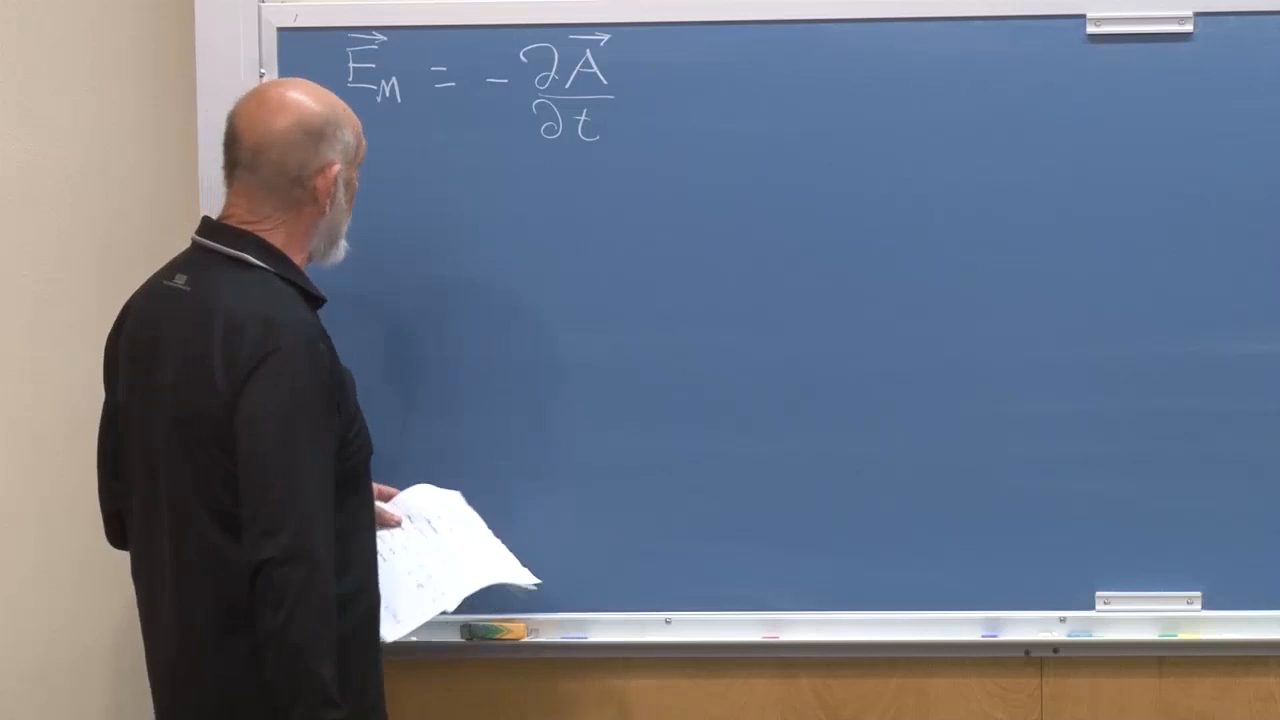
\includegraphics[width=\linewidth]{lecture_10_figure_02.png}\caption{Einführung des mechanischen Impulses als Masse mal Schwerpunktgeschwindigkeit.}\par\smallskip
\textit{Vorlesungsbild: 00:11:15.}\end{figure}

\subsection{Kanonischer Impuls}

Angenommen, die Mechanik wird beschrieben durch
\(L(q_i,\dot q_i)\). Der zu \(q_i\) kanonisch konjugierte Impuls ist
\begin{equation}
p_i=\frac{\partial L}{\partial\dot q_i}.
\label{eq:canonical-momentum}
\end{equation}
Für
\begin{equation}
L=\frac12 m\dot{\mathbf x}^{\,2}-V(\mathbf x),
\label{eq:simple-particle-lagrangian}
\end{equation}
ergibt sich damit \(\mathbf p=m\dot{\mathbf x}\); kanonischer und mechanischer Impuls stimmen hier also zufällig überein.

\begin{figure}[H]\centering
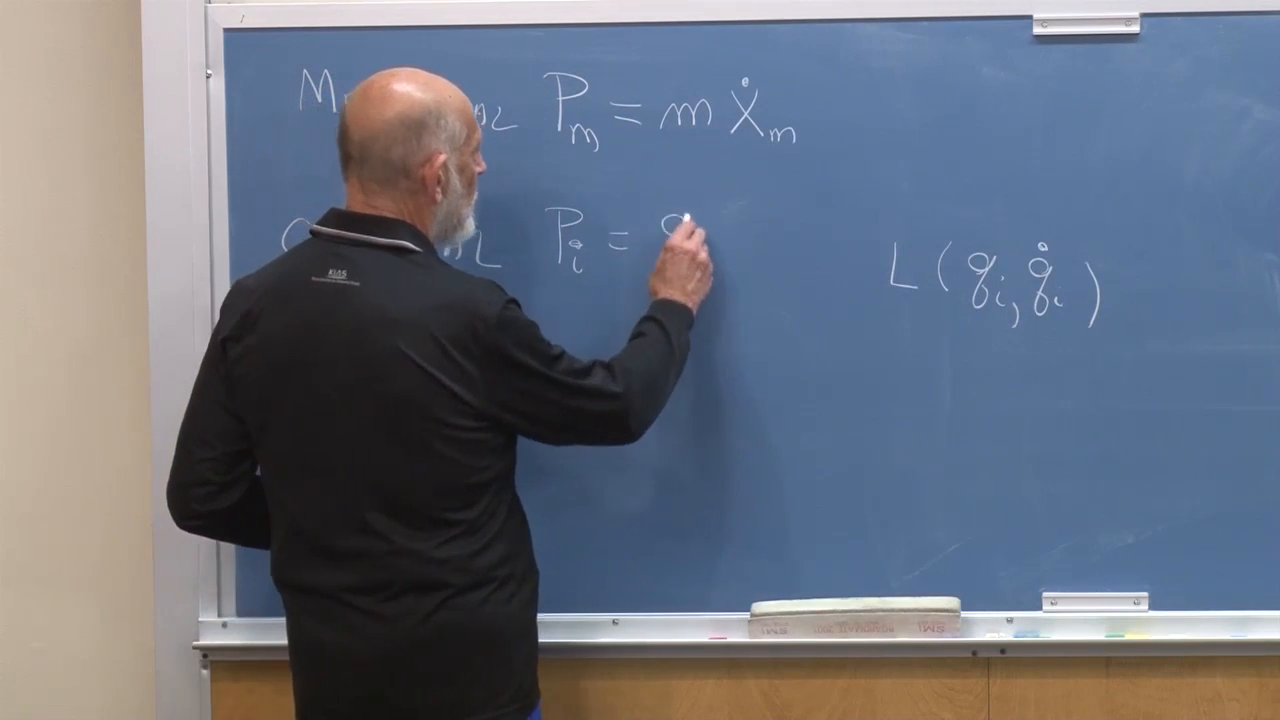
\includegraphics[width=\linewidth]{lecture_10_figure_03.png}\caption{Mechanischer und kanonischer Impuls neben der einfachen Teilchen-Lagrange-Funktion.}\par\smallskip
\textit{Vorlesungsbild: 00:13:40.}\end{figure}

Ein geladenes Teilchen in einem Magnetfeld ist das nützliche Gegenbeispiel. Mit der an der Tafel angegebenen Vorzeichenkonvention gilt
\begin{equation}
L=\frac12m\dot{\mathbf x}^{\,2}-V(\mathbf x)
  -e\,\dot{\mathbf x}\cdot\mathbf A(\mathbf x),
\label{eq:magnetic-particle-lagrangian}
\end{equation}
und daher
\begin{equation}
p_i=m\dot x_i-eA_i.
\label{eq:magnetic-canonical-shift}
\end{equation}
Eine Änderung der Ladungskonvention oder des Vorzeichens des Wechselwirkungsterms ändert das angezeigte Vorzeichen, nicht aber die Lehre: Der kanonische Impuls enthält einen Beitrag des Vektorpotentials und ist nicht einfach \(m\dot x_i\). Hamilton-Gleichungen verwenden die kanonische Variable. Später kann man den feldabhängigen Term auf die andere Seite einer Gleichung bringen und so eine Newton ähnlich sehende Beschleunigungsgleichung erhalten; diese Umformung ändert jedoch nicht die Definition.

\begin{figure}[H]\centering
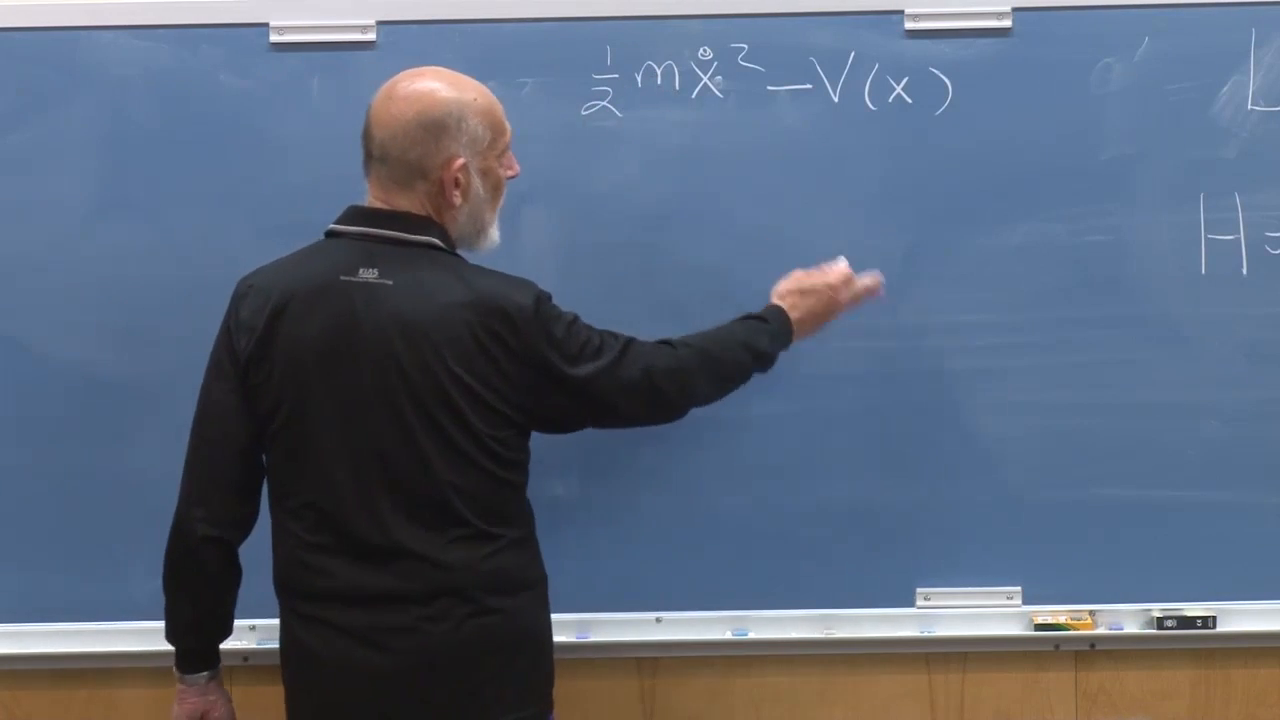
\includegraphics[width=\linewidth]{lecture_10_figure_04.png}\caption{Der Beitrag des Vektorpotentials verschiebt den kanonischen Impuls gegenüber dem mechanischen Impuls.}\par\smallskip
\textit{Vorlesungsbild: 00:15:50.}\end{figure}

\subsection{Noether-Impuls}

Der dritte Impuls ist die erhaltene Ladung, die mit der Invarianz unter räumlichen Translationen verbunden ist. Für eine infinitesimale Symmetrie
\begin{equation}
q_i\longrightarrow q_i+\delta q_i
\end{equation}
die die Lagrange-Funktion invariant lässt, ergibt der Noether-Satz bis auf die Normierung des infinitesimalen Parameters
\begin{equation}
Q=\sum_i p_i\,\delta q_i.
\label{eq:noether-charge-mechanics}
\end{equation}
Die hier auftretenden \(p_i\) sind kanonische Impulse. Ist die Symmetrie eine gleichförmige Translation und stimmt der kanonische Impuls zufällig mit dem mechanischen Impuls überein, dann ergibt sich aus \(Q\) der bekannte Gesamtimpuls. In einem weniger einfachen System muss diese Übereinstimmung bewiesen werden; man darf sie nicht voraussetzen.

\begin{figure}[H]\centering
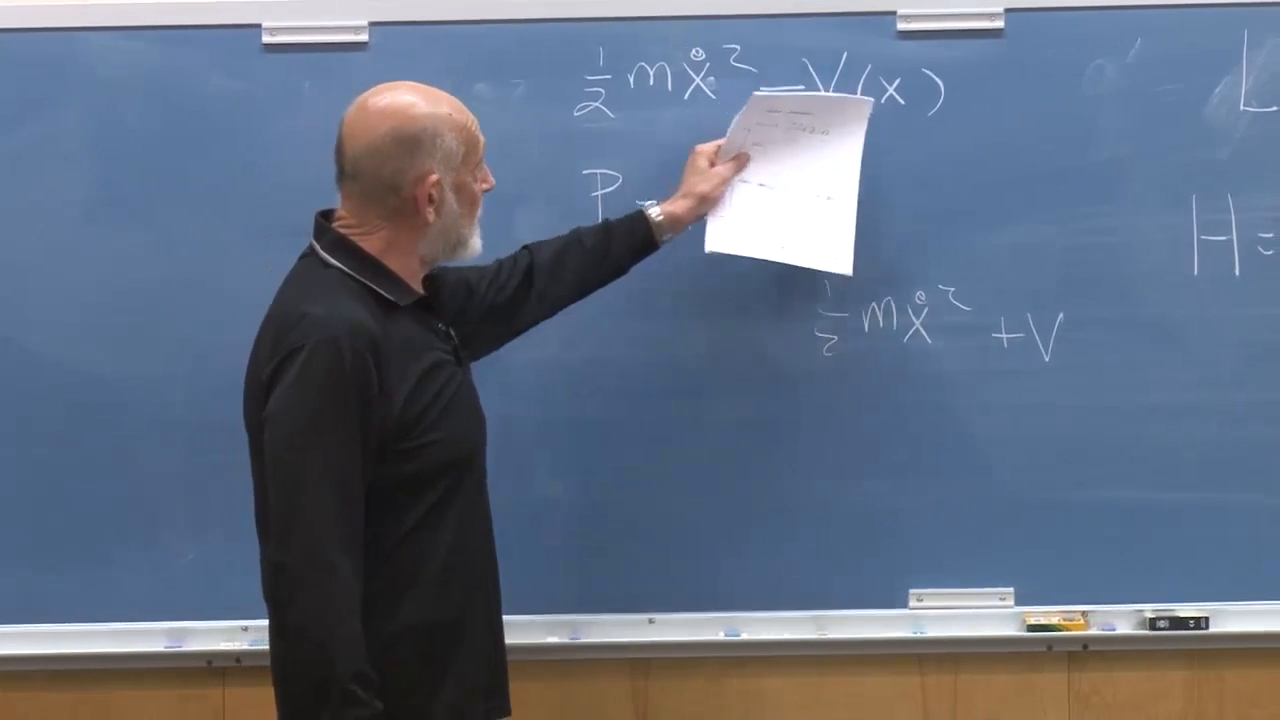
\includegraphics[width=\linewidth]{lecture_10_figure_05.png}\caption{Die Noether-Ladung, zusammengesetzt aus kanonischen Impulsen und den infinitesimalen Änderungen der Koordinaten.}\par\smallskip
\textit{Vorlesungsbild: 00:19:00.}\end{figure}

\section{Energie als Hamilton-Funktion}

Räumliche Translationen führen zum Impuls, zeitliche Translationen zur Energie. Hängt die Lagrange-Funktion nicht explizit von der Zeit ab, so ist die Hamilton-Funktion
\begin{equation}
H=\sum_i p_i\dot q_i-L
\label{eq:hamiltonian-definition}
\end{equation}
erhalten. Sie ist die Legendre-Transformation der Lagrange-Funktion und keine Regel, nach der man Vorzeichen durch bloßes Hinsehen ändert.

\begin{figure}[H]\centering
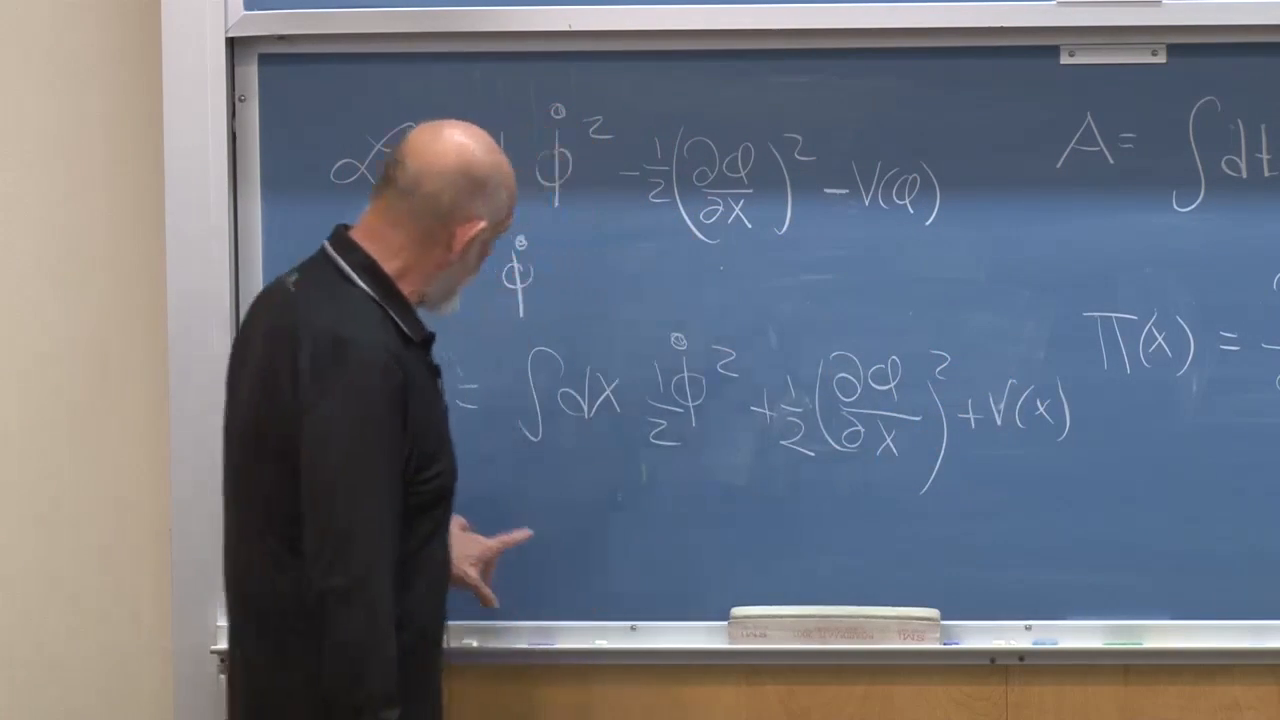
\includegraphics[width=\linewidth]{lecture_10_figure_06.png}\caption{Die Hamilton-Funktion als Legendre-Transformation einer allgemeinen Lagrange-Funktion.}\par\smallskip
\textit{Vorlesungsbild: 00:22:55.}\end{figure}

Für das Beispiel mit einem Teilchen gilt
\begin{align}
p&=m\dot x,
\nonumber\\
H&=p\dot x-L\\
&=m\dot x^2
  -\left(\frac12m\dot x^2-V(x)\right)\\
&=\frac12m\dot x^2+V(x).
\label{eq:particle-hamiltonian}
\end{align}
Die Lagrange-Funktion ist also kinetische minus potenzielle Energie, während die Hamilton-Funktion kinetische plus potenzielle Energie ist.

\begin{figure}[H]\centering
\includegraphics[width=\linewidth]{lecture_10_figure_07.png}\caption{Die Teilchenrechnung zeigt, wie \(H=T+V\) aus \(H=p\dot x-L\) folgt.}\par\smallskip
\textit{Vorlesungsbild: 00:24:20.}\end{figure}

Wenn jede Geschwindigkeitsabhängigkeit ein übliches positives quadratisches kinetisches Glied ist und der übrige Teil keine Geschwindigkeiten enthält, lässt sich die Hamilton-Funktion direkt ablesen, indem man das Vorzeichen des geschwindigkeitsunabhängigen Teils umkehrt. Diese Abkürzung werden wir wiederholt verwenden. Sie ist nur deshalb zulässig, weil die Legendre-Transformation in den betrachteten Beispielen diese einfache Form hat.

\section{Ein Feld ist ein mechanisches System mit unendlich vielen Koordinaten}

Um die mechanische Struktur der Feldtheorie sichtbar zu machen, wählen wir ein Inertialsystem und bestehen vorübergehend nicht darauf, dass jede Zeile manifest Lorentz-kovariant ist. Die klassische Mechanik hat eine Zeitachse und Koordinaten \(q_i(t)\). Ein Skalarfeld hat eine Zeitachse und Koordinaten \(\phi(\mathbf x,t)\). Die diskrete Bezeichnung \(i\) ist einfach zur kontinuierlichen Bezeichnung \(\mathbf x\) geworden:
\begin{equation}
q_i(t)\quad\longrightarrow\quad\phi(\mathbf x,t).
\label{eq:discrete-to-field}
\end{equation}
Der Feldwert an jedem Raumpunkt ist ein Freiheitsgrad. Hier bezeichnet \(\mathbf x\), welcher Freiheitsgrad gemeint ist; die Ortskoordinate ist nicht selbst die verallgemeinerte Koordinate.

\begin{figure}[H]\centering
\includegraphics[width=\linewidth]{lecture_10_figure_08.png}\caption{Ein räumliches Gitter, auf dem der Feldwert an jedem Punkt als eigener mechanischer Freiheitsgrad dargestellt wird.}\par\smallskip
\textit{Vorlesungsbild: 00:30:15.}\end{figure}

\begin{classroomqa}\audiencequestion{Warum schreiben wir das Feld nicht gleich als \(\phi(\mathbf x,t)\)?}\lecturerresponse{Das ist die vollständige Notation. Die vorübergehende Schreibweise \(\phi(\mathbf x)\) lässt das gemeinsame Zeitargument weg, so wie man oft \(q_i\) schreibt und dabei im Kopf behält, dass jedes \(q_i\) von der Zeit abhängt. Die Bezeichnung \(i\) oder nun \(\mathbf x\) gibt an, welcher Freiheitsgrad betrachtet wird. \lecturetimestamp{00:32:43}}\end{classroomqa}

\begin{classroomqa}\audiencequestion{Sind die Feldwerte an benachbarten Punkten wirklich unabhängige Koordinaten? Was erzwingt ihre Stetigkeit?}\lecturerresponse{Sie sind unabhängige kanonische Koordinaten. Glattheit wird nicht dadurch erzwungen, dass benachbarte Werte gleichgesetzt werden; sie ergibt sich dynamisch. Die Hamilton-Funktion enthält ein positives Gradientenenergieglied. Daher kostet ein fester Sprung über eine immer kleinere Entfernung immer mehr Energie. Konfigurationen endlicher Energie sind im Kontinuumslimes folglich glatt. \lecturetimestamp{00:33:09}}\end{classroomqa}

Eine räumliche Ableitung macht die Kopplung benachbarter Freiheitsgrade explizit. Auf einem Gitter mit Gitterabstand \(\epsilon\) gilt
\begin{equation}
\partial_x\phi(x,t)
  =\lim_{\epsilon\to0}
   \frac{\phi(x+\epsilon,t)-\phi(x,t)}{\epsilon}.
\label{eq:field-finite-difference}
\end{equation}
Sie hängt von zwei benachbarten Koordinaten ab, enthält aber keine verallgemeinerte Geschwindigkeit. In der mechanischen Analogie gehört sie zur Koordinatenabhängigkeit der Lagrange-Funktion, nicht zur Abhängigkeit von \(\dot q_i\).

\begin{figure}[H]\centering
\includegraphics[width=\linewidth]{lecture_10_figure_09.png}\caption{Die räumliche Ableitung, rekonstruiert als Differenz benachbarter Feldwerte auf dem Gitter.}\par\smallskip
\textit{Vorlesungsbild: 00:31:40.}\end{figure}

Die Wirkung lässt sich nun in ausdrücklich mechanischer Form schreiben:
\begin{align}
S&=\int dt\,L,
\nonumber\\
L&=\int d^3x\,
\mathcal L\!\left(
\phi,\dot\phi,\boldsymbol{\nabla}\phi
\right),
\nonumber\\
S&=\int dt\,d^3x\,
\mathcal L\!\left(
\phi,\dot\phi,\boldsymbol{\nabla}\phi
\right).
\label{eq:field-action-split}
\end{align}
Der kalligrafische Buchstabe \(\mathcal L\) bezeichnet die Lagrange-Dichte; ihre Integration über den Raum ergibt die gewöhnliche Lagrange-Funktion, die über die Zeit integriert wird. Eine lokale Theorie koppelt jeden Punkt nur über die Felder und ihre Ableitungen an diesem Punkt. Die Aufspaltung von Zeit und Raum verbirgt vorübergehend die Lorentz-Kovarianz, macht aber die mechanische Struktur durchsichtig.

\begin{figure}[H]\centering
\includegraphics[width=\linewidth]{lecture_10_figure_10.png}\caption{Die Feldwirkung, aufgeteilt in ein Zeitintegral und ein Raumintegral über die Lagrange-Dichte.}\par\smallskip
\textit{Vorlesungsbild: 00:36:40.}\end{figure}

\section{Kanonischer Feldimpuls und Hamilton-Dichte}

Die Geschwindigkeit einer Feldkoordinate ist \(\dot\phi(\mathbf x,t)\): Sie gibt an, wie sich das Feld mit der Zeit an einem festen Punkt ändert. Sie beschreibt keine Bewegung von einem Raumpunkt zu einem anderen. Der zum Feld kanonisch konjugierte Impuls ist daher selbst ein Feld:
\begin{equation}
\Pi(\mathbf x,t)
 =\frac{\partial\mathcal L}{\partial\dot\phi(\mathbf x,t)}.
\label{eq:field-canonical-momentum}
\end{equation}
Bei mehreren Feldern \(\phi_a\) gibt es für jedes davon ein Impulsfeld \(\Pi_a\).

In der Legendre-Transformation wird die diskrete Summe durch ein Raumintegral ersetzt:
\begin{align}
H
 &=\int d^3x\,
   \left[\Pi\dot\phi-\mathcal L\right]
  =\int d^3x\,\mathcal H,
\nonumber\\
\mathcal H
 &=\Pi\dot\phi-\mathcal L .
\label{eq:field-hamiltonian-density}
\end{align}
Die Größe im Integranden ist die Energiedichte.

\begin{figure}[H]\centering
\includegraphics[width=\linewidth]{lecture_10_figure_11.png}\caption{Die Legendre-Transformation für Felder und ihre Deutung als Integral der lokalen Energiedichte.}\par\smallskip
\textit{Vorlesungsbild: 00:42:40.}\end{figure}

\begin{classroomqa}\audiencequestion{Warum darf die Ableitung der gesamten Lagrange-Funktion nach \(\dot\phi\) an einem Punkt durch die Ableitung der lokalen Dichte dort ersetzt werden?}\lecturerresponse{Man kann sich das Raumintegral als kontinuierliche Summe vorstellen. Unter der hier verwendeten Lokalitätsannahme tritt die Geschwindigkeit \(\dot\phi(\mathbf x)\) nur in dem Term auf, der zu eben diesem Punkt gehört. Die Ableitung nach genau dieser Geschwindigkeit lässt alle anderen Terme wegfallen. Räumliche Ableitungen können benachbarte Feldwerte koppeln, führen in dieser Theorie aber keine benachbarten Zeitableitungen ein. \lecturetimestamp{00:51:56}}\end{classroomqa}

\subsection{Das Skalarfeld}

Betrachten wir eine Raumdimension und setzen
\begin{equation}
\mathcal L
 =\frac12\dot\phi^2
  -\frac12(\partial_x\phi)^2
  -V(\phi).
\label{eq:scalar-field-lagrangian}
\end{equation}
Dies ist die nichtkovariante Darstellung des zuvor verwendeten Lorentz-Skalars: Das relative Minuszeichen zwischen zeitlichen und räumlichen Ableitungen stammt von der Minkowski-Metrik. Der kanonische Impuls ist
\begin{equation}
\Pi=\dot\phi,
\label{eq:scalar-pi}
\end{equation}
und die Hamilton-Funktion lautet
\begin{equation}
H=\int dx\,
\left[
\frac12\dot\phi^2
+\frac12(\partial_x\phi)^2
+V(\phi)
\right].
\label{eq:scalar-field-hamiltonian}
\end{equation}
Während der Rechnung wurde das Potential vorübergehend als \(V(x)\) bezeichnet; der Kurs korrigierte die Bezeichnung zu \(V(\phi)\). Es kann indirekt über das Feld von der Position abhängen, hat in der translationsinvarianten Theorie aber keine vorgegebene äußere Abhängigkeit von \(x\).

\begin{figure}[H]\centering
\includegraphics[width=\linewidth]{lecture_10_figure_12.png}\caption{Skalarfeld-Lagrange-Dichte, konjugierter Impuls und positive Hamilton-Funktion, gemeinsam an der Tafel zusammengestellt.}\par\smallskip
\textit{Vorlesungsbild: 00:47:05.}\end{figure}

Der gesamte Anteil ohne Zeitableitungen spielt die Rolle der potenziellen Energie. Dazu gehören sowohl \(V(\phi)\) als auch die Gradientenenergie \(\frac12(\partial_x\phi)^2\). Die Lagrange-Funktion kann positiv oder negativ sein; eine stabile Energie sollte nach unten beschränkt sein.

\begin{classroomqa}\audiencequestion{Darf das Potential \(V(\phi)\) negativ sein?}\lecturerresponse{Ja. Ist es nach unten beschränkt, kann man eine Konstante addieren, sodass sein Minimum null ist, ohne die klassische Feldgleichung zu ändern. Ein nach unten unbeschränktes Potential beschreibt eine Instabilität: Das Feld kann seine Energie unbegrenzt senken. Das stabile Vakuum ist ein konstantes Feld, das an einem Minimum des verschobenen Potentials liegt. \lecturetimestamp{00:49:03}}\end{classroomqa}

Die frühere Frage nach der Stetigkeit lässt sich nun quantitativ beantworten. Ein Sprung \(\Delta\phi\) über einen Gitterabstand \(\epsilon\) trägt bei
\begin{equation}
\frac12(\partial_x\phi)^2
\sim\frac12\left(\frac{\Delta\phi}{\epsilon}\right)^2.
\label{eq:gradient-cost}
\end{equation}
Für \(\epsilon\to0\) ergibt ein fester Sprung eine beliebig große Energiedichte. Konfigurationen mit starken Unstetigkeiten werden daher durch die endliche Energie unterdrückt.

\begin{figure}[H]\centering
\includegraphics[width=\linewidth]{lecture_10_figure_13.png}\caption{Die Skalarfeld-Energieformel bleibt stehen, während die Skizze an der Tafel ein glattes Feld einer abrupten Änderung gegenüberstellt.}\par\smallskip
\textit{Vorlesungsbild: 00:54:20.}\end{figure}

\section{Lokale Energie und die Bedeutung von \texorpdfstring{\(T^{00}\)}{T00}}

Die Energiedichte erhält eine kompakte Bezeichnung:
\begin{equation}
T^{00}=\mathcal H=\Pi\dot\phi-\mathcal L.
\label{eq:T00-definition}
\end{equation}
Die beiden Nullindizes drücken zwei verschiedene Aussagen aus. Energie ist die Zeitkomponente \(P^0\) des Energie--Impuls-Vierervektors, während eine Dichte die Zeitkomponente eines Erhaltungsstroms ist. Somit ist \(T^{00}\) die Dichte der Zeitkomponente des Viererimpulses.

\begin{figure}[H]\centering
\includegraphics[width=\linewidth]{lecture_10_figure_14.png}\caption{Das Feldenergie-Integral wird lokal geschrieben und mit \(T^{00}\) identifiziert.}\par\smallskip
\textit{Vorlesungsbild: 01:00:00.}\end{figure}

Erhaltung in einer relativistischen lokalen Theorie bedeutet mehr, als dass eine globale Zahl unverändert bleibt. Energie kann nicht im Labor verschwinden und bei Alpha Centauri wieder auftauchen. Eine Änderung innerhalb eines Gebiets muss durch einen Fluss über dessen Rand erklärt werden. In lokaler Form gilt
\begin{equation}
\partial_\mu T^{\mu\nu}=0,
\label{eq:stress-energy-continuity}
\end{equation}
Der erste Index bezeichnet also die Dichte oder die Flussrichtung, der zweite gibt an, welche Komponente \(P^\nu\) transportiert wird.

\begin{classroomqa}\audiencequestion{Bedeutet die Bezeichnung \(T^{00}\) als Dichte, dass man die Gesamtenergie durch Integration darüber erhält?}\lecturerresponse{Genau:
\(E=P^0=\int d^3x\,T^{00}\). Die lokale Dichte steht als Integrand in der Legendre-Transformation des Feldes. Eine Änderung an einem Ort wird durch einen Energiestrom zwischen benachbarten Orten ausgeglichen. \lecturetimestamp{00:59:06}}\end{classroomqa}

\section{Impulsdichte aus räumlichen Translationen}

Kehren wir zur Noether-Formel zurück und ersetzen nun die diskrete Summe durch ein Raumintegral. Bei einer kleinen Translation in \(m\)-Richtung ändert sich das Feld gemäß
\begin{equation}
\delta\phi
  =\phi(\mathbf x)-\phi(\mathbf x-\boldsymbol{\epsilon})
  =\epsilon^m\partial_m\phi+O(\epsilon^2),
\label{eq:translated-field-change}
\end{equation}
für die an der Tafel verwendete passive Konvention. Bei einem Wechsel zwischen aktiven und passiven Translationen kehrt sich das Gesamtvorzeichen um; sobald diese Konvention festgelegt ist, steht auch der physikalische Erzeuger fest. Klammert man \(\epsilon^m\) aus, hat der Noether-Impuls die Form
\begin{equation}
P_m\ \propto\ \int d^3x\,\Pi\,\partial_m\phi.
\label{eq:scalar-noether-momentum}
\end{equation}

\begin{figure}[H]\centering
\includegraphics[width=\linewidth]{lecture_10_figure_15.png}\caption{Ein verschobenes Feldprofil und die Ableitung, die seine infinitesimale Änderung misst.}\par\smallskip
\textit{Vorlesungsbild: 01:04:20.}\end{figure}

\begin{classroomqa}\audiencequestion{Warum blieb die infinitesimale Translation \(\epsilon\) nicht in der Impulsformel stehen?}\lecturerresponse{Die Noether-Ladung ergibt sich zunächst proportional zu \(\epsilon\). Der Impuls ist als Koeffizient dieses beliebigen Translationsparameters definiert, daher wird \(\epsilon\) herausgekürzt. Eine erhaltene Größe mit einer festen Konstante zu multiplizieren, würde an ihrer Erhaltung nichts ändern; durch das Herausziehen des Koeffizienten erhält man jedoch die übliche Normierung. \lecturetimestamp{01:04:45}}\end{classroomqa}

\begin{classroomqa}\audiencequestion{Wird das Translationsintervall im Kontinuumsintegral zu \(dx\)?}\lecturerresponse{Sie stammen aus unterschiedlichen Grenzübergängen. Das Maß \(dx\) ergibt sich, wenn die Summe über räumlich bezeichnete Freiheitsgrade durch ein Integral ersetzt wird. Der Translationsparameter \(\epsilon\) beschreibt die Symmetrieoperation und wird aus ihrer Noether-Ladung ausgeklammert. In der Zwischenrechnung sind beide infinitesimal, erfüllen aber unterschiedliche Aufgaben. \lecturetimestamp{01:05:16}}\end{classroomqa}

In der Notation der Vorlesung lautet die Dichte der \(m\)-Komponente des Impulses
\begin{equation}
T^{0m}=\Pi\,\partial_m\phi,
\label{eq:scalar-momentum-density}
\end{equation}
bei vorausgesetzter Vorzeichenkonvention für Translationen. Für die Skalarfeldtheorie gilt \(\Pi=\dot\phi\), sodass sie proportional zu \(\dot\phi\,\partial_m\phi\) ist.

\begin{figure}[H]\centering
\includegraphics[width=\linewidth]{lecture_10_figure_16.png}\caption{Die Noether-Impulsdichte \(T^{0m}=\Pi\,\partial_m\phi\) an der Tafel.}\par\smallskip
\textit{Vorlesungsbild: 01:07:10.}\end{figure}

Das ist ein Impuls, den eine Welle tatsächlich trägt. Translationsinvarianz gilt nur, wenn alles verschoben wird: Felder, Teilchen, Quellen und Apparaturen. Wird ein Lichtpuls von einer frei aufgehängten Platte absorbiert, erhält die Platte einen Rückstoß. Bei gewöhnlichem Licht ist der Effekt winzig; ein ausreichend leistungsstarker Laser kann jedoch genügend Impuls übertragen, um ein kleines Ziel zu komprimieren. Der erhaltene Gesamtimpuls gehört den Teilchen und den Feldern gemeinsam.

\subsection{Was tritt an die Stelle der Newton-Gleichung?}

Die aus ~\eqref{eq:scalar-field-lagrangian} hergeleitete Euler--Lagrange-Gleichung für das Feld lautet
\begin{equation}
\ddot\phi-\nabla^2\phi=-\frac{dV}{d\phi}.
\label{eq:scalar-equation-of-motion}
\end{equation}
Sie ist das Analogon des Newtonschen Gesetzes in der Feldtheorie.

\begin{figure}[H]\centering
\includegraphics[width=\linewidth]{lecture_10_figure_17.png}\caption{Die Skalarfeldgleichung neben ihrer Hamilton-Funktion und Impulsdichte.}\par\smallskip
\textit{Vorlesungsbild: 01:12:55.}\end{figure}

\begin{classroomqa}\audiencequestion{Was entspricht dem Newtonschen Gesetz für ein Feld?}\lecturerresponse{Das leistet die Euler--Lagrange-Gleichung für das Feld. Hier ist sie eine Wellengleichung mit dem Kraftterm \(-V'(\phi)\). Die Rolle von \(m\ddot x=-V'(x)\) übernimmt \(\ddot\phi-\nabla^2\phi=-V'(\phi)\). \lecturetimestamp{01:11:48}}\end{classroomqa}

\begin{classroomqa}\audiencequestion{Woher wissen wir, ob eine vorgeschlagene Feld-Lagrange-Funktion richtig ist? Müssen wir die Feldgleichung bereits kennen?}\lecturerresponse{Beide Richtungen sind möglich. Historisch kann man aus Experimenten Gleichungen erschließen und anschließend nach einer Wirkung suchen, wie es bei Newton und Maxwell geschah. In der modernen Theorie geht man oft vom Feldinhalt, der Lokalität, der Symmetrie und einer kleinen Menge zulässiger Terme aus, leitet daraus die Gleichungen her und prüft ihre Vorhersagen. Das dargestellte Skalarfeld könnte ein fundamentales Feld beschreiben, aber ebenso die Querverschiebung eines Seils, dessen Kontinuumswirkung aus seinen Teilchen hergeleitet wird. \lecturetimestamp{01:12:55}}\end{classroomqa}

\section{Das elektromagnetische Feld in zeitlicher Eichung}

Die bereits gefundenen Komponenten \(T^{00}\) und \(T^{0m}\) gehören zum Energie--Impuls-Tensor. Seine übrigen Komponenten beschreiben Energie- und Impulsflüsse. Dieser Tensor wird später als Quelle der Gravitation dienen; das unmittelbare Beispiel liefert jedoch der Elektromagnetismus.

Die grundlegende elektromagnetische Koordinate ist das Viererpotential \(A_\mu\). Die Eichfreiheit erlaubt die Transformation
\begin{equation}
A_\mu\longrightarrow A'_\mu=A_\mu+\partial_\mu S
\label{eq:gauge-transformation-lecture10}
\end{equation}
ohne \(F_{\mu\nu}\) zu ändern. Wählen wir \(S\) so, dass
\begin{equation}
\partial_tS=-A_0.
\label{eq:temporal-gauge-choice}
\end{equation}
Zum Beispiel kann man \(A_0\) an jedem festen Raumpunkt über die Zeit integrieren. Dann verschwindet die transformierte Zeitkomponente:
\begin{equation}
A'_0=A_0+\partial_tS=0.
\label{eq:temporal-gauge}
\end{equation}
Das ist die zeitliche Eichung. Sie entfernt \(A_0\) aus der Menge der dynamischen Koordinaten, doch das Gaußsche Gesetz bleibt als Zwangsbedingung bestehen, ebenso eine zeitunabhängige Resteichfreiheit.

\begin{figure}[H]\centering
\includegraphics[width=\linewidth]{lecture_10_figure_18.png}\caption{Die Eichfreiheit wird genutzt, um \(A_0=0\) durch Lösung von \(\partial_tS=-A_0\) zu wählen.}\par\smallskip
\textit{Vorlesungsbild: 01:20:15.}\end{figure}

Von jetzt an bezeichne \(\mathbf E\) das Standardfeld von Maxwell. Vor der Eichfixierung gilt
\begin{equation}
E_m=-\partial_tA_m+\partial_mA_0,
\qquad
\mathbf B=\boldsymbol{\nabla}\times\mathbf A.
\label{eq:E-B-general-potential}
\end{equation}
In zeitlicher Eichung vereinfacht sich dies zu
\begin{equation}
\mathbf E=-\dot{\mathbf A},
\qquad
\mathbf B=\boldsymbol{\nabla}\times\mathbf A.
\label{eq:E-B-temporal-gauge}
\end{equation}
Zeitableitungen von \(\mathbf A\) ergeben das elektrische Feld; räumliche Ableitungen ergeben das Magnetfeld.

\begin{figure}[H]\centering
\includegraphics[width=\linewidth]{lecture_10_figure_19.png}\caption{Elektrisches und magnetisches Feld in zeitlicher Eichung: \(\mathbf E=-\dot{\mathbf A}\) und \(\mathbf B=\nabla\times\mathbf A\).}\par\smallskip
\textit{Vorlesungsbild: 01:23:50.}\end{figure}

\section{Kanonischer Impuls und Energie des elektromagnetischen Feldes}

Die freie Lagrange-Dichte von Maxwell lautet
\begin{equation}
\mathcal L_{\mathrm{EM}}
 =-\frac14F_{\mu\nu}F^{\mu\nu}
 =\frac12\left(\mathbf E^2-\mathbf B^2\right).
\label{eq:maxwell-lagrangian-energy-lecture}
\end{equation}
In zeitlicher Eichung gilt
\begin{equation}
\mathcal L_{\mathrm{EM}}
 =\frac12\dot{\mathbf A}^{\,2}
  -\frac12(\boldsymbol{\nabla}\times\mathbf A)^2.
\label{eq:maxwell-lagrangian-temporal}
\end{equation}
Sie hat genau die Form des Skalarfelds: Quadrate der Zeitableitungen minus Quadrate der räumlichen Ableitungen.

\begin{figure}[H]\centering
\includegraphics[width=\linewidth]{lecture_10_figure_20.png}\caption{Die Lagrange-Funktion von Maxwell, umgeschrieben als mechanische Feld-Lagrange-Funktion für die räumlichen Komponenten von \(\mathbf A\).}\par\smallskip
\textit{Vorlesungsbild: 01:28:10.}\end{figure}

Zu jeder Komponente \(A_m\) gehört ein kanonischer Impuls:
\begin{equation}
\Pi_m
 =\frac{\partial\mathcal L_{\mathrm{EM}}}
        {\partial\dot A_m}
 =\dot A_m
 =-E_m.
\label{eq:em-canonical-momentum}
\end{equation}
Das ist ein konkretes Beispiel dafür, warum die Konvention wichtig ist. Bei der zuvor verwendeten entgegengesetzten Konvention für das elektrische Feld würde sich das Vorzeichen in der letzten dargestellten Gleichung ändern, die kanonische Ableitung selbst jedoch nicht.

\begin{figure}[H]\centering
\includegraphics[width=\linewidth]{lecture_10_figure_21.png}\caption{Die drei kanonischen Impulsfelder zu \(A_x,A_y,A_z\) sind jeweils gleich der entsprechenden Zeitableitung und damit gleich dem negativen Standard-Elektrofeld.}\par\smallskip
\textit{Vorlesungsbild: 01:30:20.}\end{figure}

Die Abkürzung für die Hamilton-Funktion ist nun begründet: Man kehrt das Vorzeichen des Terms ohne Zeitableitungen um. Die elektromagnetische Energiedichte ist
\begin{equation}
T^{00}_{\mathrm{EM}}
 =\mathcal H_{\mathrm{EM}}
 =\frac12\left(\mathbf E^2+\mathbf B^2\right),
\label{eq:em-energy-density}
\end{equation}
und die Gesamtenergie lautet
\begin{equation}
H_{\mathrm{EM}}
 =\int d^3x\,
\frac12\left(\mathbf E^2+\mathbf B^2\right).
\label{eq:em-total-energy}
\end{equation}
Anders als die Lagrange-Dichte ist die Energiedichte nichtnegativ.

\begin{figure}[H]\centering
\includegraphics[width=\linewidth]{lecture_10_figure_22.png}\caption{Die positive elektromagnetische Hamilton-Dichte \(\frac12(\mathbf E^2+\mathbf B^2)\).}\par\smallskip
\textit{Vorlesungsbild: 01:32:00.}\end{figure}

Für eine ebene Welle im Vakuum gilt \(\mathbf E\perp\mathbf B\); die beiden Felder sind phasengleich und haben in Einheiten mit \(c=1\) den gleichen Betrag. Daher tragen das elektrische und das magnetische Feld jeweils gleich viel zur Wellenenergie bei:
\begin{equation}
u_E=\frac12\mathbf E^2,
\qquad
u_B=\frac12\mathbf B^2,
\qquad
u_E=u_B.
\label{eq:plane-wave-energy-halves}
\end{equation}

\section{Herleitung des elektromagnetischen Impulses}

Die Noether-Formel für Translationen muss nun über die drei Felder \(A_m\) summiert werden. Wählt man das Vorzeichen der Translation so, dass der physikalische Impuls in Ausbreitungsrichtung zeigt, lautet die \(n\)-Komponente
\begin{equation}
P_n
 =\int d^3x\,E_m\,\partial_nA_m,
\label{eq:em-canonical-noether-momentum}
\end{equation}
wobei über \(m\) summiert wird. Die Vorlesung hält ausdrücklich beim Vorzeichen inne: Es hängt von den zuvor gewählten Konventionen für das elektrische Feld sowie für aktive und passive Translationen ab. Das eichinvariante physikalische Ergebnis wird das Vorzeichen festlegen.

\begin{figure}[H]\centering
\includegraphics[width=\linewidth]{lecture_10_figure_23.png}\caption{Die Noether-Formel für das Skalarfeld, erweitert auf die drei Komponenten des Vektorpotentials.}\par\smallskip
\textit{Vorlesungsbild: 01:36:40.}\end{figure}

Der Integrand enthält nach wie vor das Eichpotential und nicht nur die physikalischen Felder. Addiert und subtrahiert man \(E_m\partial_mA_n\), erhält man:
\begin{align}
E_m\partial_nA_m
 &=
 E_m\left(\partial_nA_m-\partial_mA_n\right)
 +E_m\partial_mA_n.
\label{eq:add-subtract-em-momentum}
\end{align}
Der erste Term ist ein Kreuzprodukt:
\begin{equation}
E_m\left(\partial_nA_m-\partial_mA_n\right)
  =(\mathbf E\times\mathbf B)_n.
\label{eq:cross-product-component}
\end{equation}
Beim zweiten Term integrieren wir partiell:
\begin{align}
\int d^3x\,E_m\partial_mA_n
 &=
\int_{\partial V}d\Sigma_m\,E_mA_n
-\int d^3x\,A_n\partial_mE_m.
\label{eq:em-momentum-integration-parts}
\end{align}
Fallen die Felder so ab, dass der Randterm verschwindet, und ist das Gebiet quellenfrei, sodass \(\boldsymbol{\nabla}\cdot\mathbf E=0\) gilt, trägt der zweite Term nichts bei.

\begin{figure}[H]\centering
\includegraphics[width=\linewidth]{lecture_10_figure_24.png}\caption{Der hinzugefügte Term, der durch partielle Integration zu \(\nabla\cdot\mathbf E\) übergeht.}\par\smallskip
\textit{Vorlesungsbild: 01:40:00.}\end{figure}

Der Gesamtimpuls des Feldes lautet daher
\begin{equation}
\mathbf P_{\mathrm{EM}}
 =\int d^3x\,\mathbf E\times\mathbf B,
\qquad
\mathbf g_{\mathrm{EM}}
 =\mathbf E\times\mathbf B,
\label{eq:em-momentum-density}
\end{equation}
in den Einheiten der Vorlesung. Der Vektor \(\mathbf g_{\mathrm{EM}}\) ist die elektromagnetische Impulsdichte.

\begin{figure}[H]\centering
\includegraphics[width=\linewidth]{lecture_10_figure_25.png}\caption{Der Ausdruck mit dem Eichpotential wird zum eichinvarianten Impuls \(\int d^3x\,\mathbf E\times\mathbf B\) vereinfacht.}\par\smallskip
\textit{Vorlesungsbild: 01:41:10.}\end{figure}

\begin{classroomqa}\audiencequestion{Wo wurde \(\boldsymbol{\nabla}\cdot\mathbf E=0\) verwendet, und was gilt bei vorhandenen Ladungen?}\lecturerresponse{Nach der partiellen Integration lässt sich damit der Volumenterm beseitigen; die dargestellte Herleitung, die nur Felder enthält, gilt also für eine freie elektromagnetische Welle. Sind Ladungen vorhanden, verschwindet dieser Term nicht, und der Impuls der geladenen Materie muss einbezogen werden. Translationsinvarianz und Impulserhaltung beziehen sich auf das vollständige System aus Materie--und Feld. \lecturetimestamp{01:41:55}}\end{classroomqa}

\subsection{Richtung des Wellenimpulses}

In einer ebenen Welle bilden \(\mathbf E\), \(\mathbf B\) und die Ausbreitungsrichtung ein rechtshändiges Dreibein. Eine halbe Wellenlänge später kehren sich sowohl \(\mathbf E\) als auch \(\mathbf B\) um:
\begin{equation}
(-\mathbf E)\times(-\mathbf B)
 =\mathbf E\times\mathbf B.
\label{eq:poynting-sign-reversal}
\end{equation}
Die Impulsdichte zeigt daher während der gesamten Schwingung in eine feste Richtung: in die Ausbreitungsrichtung der Welle.

\begin{figure}[H]\centering
\includegraphics[width=\linewidth]{lecture_10_figure_26.png}\caption{Geometrie der ebenen Welle: Elektrisches und magnetisches Feld kehren sich gemeinsam um, während ihr Kreuzprodukt weiterhin entlang der Ausbreitungsachse zeigt.}\par\smallskip
\textit{Vorlesungsbild: 01:43:10.}\end{figure}

Deshalb übt Lichtdruck eine reale Wirkung aus. Bei der Absorption wird der Feldimpuls auf Materie übertragen; bei der Reflexion kehrt sich der Lichtimpuls um, sodass auf den Reflektor die doppelte Normalkomponente übertragen werden kann.

\section{Wo das Potential mit den beobachtbaren Feldern verknüpft ist}

Zum Abschluss fragt die Klasse nach den Berührungspunkten zwischen \(A_\mu\) und den beobachtbaren Feldern. Es sind genau die folgenden:
\begin{align}
E_n&=-\partial_tA_n+\partial_nA_0,
\nonumber\\
B_n&=\epsilon_{nmk}\partial_mA_k.
\label{eq:potential-field-contact}
\end{align}
Die Eichung mit verschwindendem Skalarpotential beseitigt den Term \(A_0\), ändert aber nicht die physikalischen Felder.

\begin{figure}[H]
\centering
\includegraphics[width=\linewidth]{lecture_10_figure_27.png}
\caption{Die allgemeine Beziehung für das elektrische Feld, die nach der Rechnung in der Eichung mit verschwindendem Skalarpotential wieder eingesetzt wird, zusammen mit der kovarianten skalaren Lagrange-Dichte, an die darunter erinnert wird.}
\par\smallskip
\textit{Vorlesungszeit: 01:45:40.}
\end{figure}

\begin{classroomqa}
\audiencequestion{Wo genau besteht der Zusammenhang zwischen dem Vektorpotential und den elektrischen und magnetischen Feldern?}
\lecturerresponse{Das elektrische Feld setzt sich aus der Zeitableitung des räumlichen Potentials und der räumlichen Ableitung von \(A_0\) zusammen; das magnetische Feld ist die Rotation des räumlichen Potentials. In der Eichung mit verschwindendem Skalarpotential vereinfacht sich dies zu
\(\mathbf E=-\dot{\mathbf A}\) und
\(\mathbf B=\nabla\times\mathbf A\).
\lecturetimestamp{01:44:15}}
\end{classroomqa}

\begin{classroomqa}
\audiencequestion{Ist das Potential fundamentaler als \(\mathbf E\) und \(\mathbf B\)?}
\lecturerresponse{Die Wirkung und das Eichprinzip lassen sich am natürlichsten mit \(A_\mu\) formulieren, wodurch dem Potential eine grundlegende strukturelle Rolle zukommt. Doch \(A_\mu\) ist nicht eindeutig: Eichverwandte Potentiale beschreiben dieselbe Physik, und die lokalen Felder sind eichinvariant. Beide Aussagen sind miteinander vereinbar. Grundlegende Variablen müssen nicht selbst unmittelbar beobachtbar sein. \lecturetimestamp{01:46:36}}
\end{classroomqa}

\begin{classroomqa}
\audiencequestion{Kann das Eichpotential selbst eine Kraft ausüben?}
\lecturerresponse{Eine eichabhängige Darstellung kann keine eichabhängige, messbare Kraft hervorrufen. Geladene Materie ist in der Wirkung über das Potential gekoppelt, doch die klassische Lorentzkraft lässt sich vollständig durch die eichinvarianten elektrischen und magnetischen Felder ausdrücken.
\lecturetimestamp{01:47:49}}
\end{classroomqa}

\begin{classroomqa}
\audiencequestion{Muss der Impuls gekreuzter elektrischer und magnetischer Felder null sein, wenn sie statisch sind?}
\lecturerresponse{Nicht unbedingt für das Feld allein:
\(\mathbf E\times\mathbf B\) kann von null verschieden sein, obwohl beide Felder zeitunabhängig sind. In einem abgeschlossenen statischen Aufbau umfasst die vollständige Impulsbilanz auch die Ladungen, Ströme, Halterungen sowie jeglichen mechanischen oder verborgenen Impuls. Die knappe Antwort aus der Vorlesung, dass sich die Gesamtbilanz ausgleichen muss, ist die richtige Aussage zur Erhaltung; allein den Feldbeitrag auf null zu setzen, wäre eine zu starke Forderung.
\lecturetimestamp{01:48:01}}
\end{classroomqa}

\section{Ein Tensor, zwei Bedeutungen des Poynting-Vektors}

Der Energie--Impuls-Tensor ordnet sämtliche Dichten und Flüsse:
\begin{align}
T^{00}&=\text{energy density},\\
T^{0i}&=\text{\(i\)-momentum density},\\
T^{i0}&=\text{energy flux in the \(i\)-direction},\\
T^{ij}&=\text{\(j\)-momentum flux in the \(i\)-direction}.
\label{eq:stress-energy-components}
\end{align}
Zum Beispiel gibt \(T^{31}\) an, wie viel \(x\)-Impuls pro Zeiteinheit eine Flächeneinheit durchquert, deren Normale in \(z\)-Richtung zeigt. Der räumliche Block \(T^{ij}\) ist der Spannungstensor.

\begin{figure}[H]
\centering
\includegraphics[width=\linewidth]{lecture_10_figure_28.png}
\caption{An der Tafel werden Dichte- und Flusskomponenten zum Energie--Impuls-Tensor angeordnet.}
\par\smallskip
\textit{Vorlesungszeit: 01:51:10.}
\end{figure}

Für die hier betrachteten relativistischen Systeme lässt sich der physikalische Energie--Impuls-Tensor symmetrisch wählen:
\begin{equation}
T^{\mu\nu}=T^{\nu\mu}.
\label{eq:stress-energy-symmetry}
\end{equation}
Daraus folgt:
\begin{equation}
T^{0i}=T^{i0}.
\label{eq:momentum-density-energy-flux}
\end{equation}
Die Dichte des \(i\)-Impulses ist gleich dem Energiefluss in \(i\)-Richtung, wenn \(c=1\) gilt. Das ist die Antwort auf eine abschließende Frage aus dem Publikum: Der Poynting-Vektor ist tatsächlich eine Leistungsdichte.

\begin{classroomqa}
\audiencequestion{Ist \(\mathbf E\times\mathbf B\) die Leistungsdichte und nicht die Impulsdichte?}
\lecturerresponse{Beides. Die Symmetrie von \(T^{\mu\nu}\) setzt die Impulsdichte \(T^{0i}\) mit dem Energiefluss \(T^{i0}\) gleich. Somit ist \(\mathbf S=\mathbf E\times\mathbf B\) Energie pro Zeiteinheit und Flächeneinheit und, in \(c=1\)-Einheiten, Impuls pro Volumeneinheit. Mit den üblichen Einheiten ergibt sich \(\mathbf g=\mathbf S/c^2\).
\lecturetimestamp{01:48:20}}
\end{classroomqa}

\begin{figure}[H]
\centering
\includegraphics[width=\linewidth]{lecture_10_figure_29.png}
\caption{Die symmetrische Tensorbeziehung setzt Impulsdichte und Energiefluss gleich; an der Tafel ist der Poynting-Vektor als Bezeichnung angegeben.}
\par\smallskip
\textit{Vorlesungszeit: 01:53:50.}
\end{figure}

\section{Die Brücke zur allgemeinen Relativitätstheorie}

Zum Abschluss führt die Vorlesung klassische Mechanik, Feldtheorie und Elektromagnetismus in einer gemeinsamen Struktur zusammen:
\begin{enumerate}
\item Zeittranslationsinvarianz liefert den Hamiltonian und die Energie.
\item Räumliche Translationsinvarianz liefert den Noether-Impuls.
\item Wer diskrete Koordinaten durch räumlich indizierte Felder ersetzt, macht aus Summen Integrale und aus Erhaltungsgrößen lokale Dichten.
\item Die Eichfixierung legt die mechanischen Koordinaten des Maxwell-Feldes offen, ohne seine Observablen zu verändern.
\item Der Maxwell-Hamiltonian liefert \(\frac12(\mathbf E^2+\mathbf B^2)\), während räumliche Translationen \(\mathbf E\times\mathbf B\) ergeben.
\item Der symmetrische Energie--Impuls-Tensor vereinigt Energiedichte, Impulsdichte, Energiefluss und Spannung.
\end{enumerate}

Diese Größe wird im nächsten Schritt benötigt. In der allgemeinen Relativitätstheorie tritt der Energie--Impuls-Tensor als Quelle in Einsteins Feldgleichung auf. Die letzte Vorlesung hat also nicht einfach noch eine elektromagnetische Rechnung angefügt, sondern die Begriffe vorbereitet, mit denen Materie und Felder der Raumzeit vorgeben, wie sie sich krümmt.

\end{document}